%% USPSC-Tutorial.tex
% ---------------------------------------------------------------
% USPSC: Modelo de Trabalho Academico (tese de doutorado, dissertacao de
% mestrado e trabalhos monograficos em geral) em conformidade com 
% ABNT NBR 14724:2011: Informacao e documentacao - Trabalhos academicos -
% Apresentacao
%----------------------------------------------------------------
%% Esta é uma customização do abntex2-modelo-trabalho-academico.tex de v-1.9.5 laurocesar 
%% para as Unidades do Campus USP de São Carlos:
%% EESC - Escola de Engenharia de São Carlos
%% IAU - Instituto de Arquitetura e Urbanismo
%% ICMC - Instituto de Ciências Matemáticas e de Computação
%% IFSC - Instituto de Física de São Carlos
%% IQSC - Instituto de Química de São Carlos
%%
%% Este trabalho utiliza a classe USPSC.cls que é mantida pela seguinte equipe:
%% 
%% Coordenação e Programação:
%%   - Marilza Aparecida Rodrigues Tognetti - marilza@sc.usp.br (PUSP-SC)
%%   - Ana Paula Aparecida Calabrez - aninha@sc.usp.br (PUSP-SC)
%% Normalização:
%%   - Brianda de Oliveira Ordonho Sigolo - brianda@usp.br (IAU)
%%   - Eduardo Graziosi Silva - edu.gs@sc.usp.br (EESC)
%%   - Eliana de Cássia Aquareli Cordeiro - eliana@iqsc.usp.br (IQSC)
%%   - Flávia Helena Cassin - cassinp@sc.usp.br (EESC)
%%   - Maria Cristina Cavarette Dziabas - mcdziaba@ifsc.usp.br (IFSC)
%%   - Regina Célia Vidal Medeiros - rcvmat@icmc.usp.br (ICMC)
%%
%% O USPSC-modelo.tex e USPSC-TCC-modelo.tex utilizam diversos arquivos relacionado em 
%% 2.1 Pacote USPSC: Classe USPSC e modelos de trabalhos acadêmicos	do Tutorial do Pascote 
%%  USPSC para modelos de trabalhos de acadêmicos em LaTeX - versão 3.0


%----------------------------------------------------------------
%% Sobre a classe abntex2.cls:
%% abntex2.cls, v-1.9.5 laurocesar
%% Copyright 2012-2015 by abnTeX2 group at https://www.abntex.net.br/ 
%%
%----------------------------------------------------------------

\documentclass[
% -- opções da classe memoir --
12pt,		% tamanho da fonte
openright,	% capítulos começam em pág ímpar (insere página vazia caso preciso)
twoside,  % para impressão em anverso (frente) e verso. Oposto a oneside - Nota: utilizar \imprimirfolhaderosto*
%oneside, % para impressão em páginas separadas (somente anverso) -  Nota: utilizar \imprimirfolhaderosto
% inclua uma % antes do comando twoside e exclua a % antes do oneside 
a4paper,			% tamanho do papel. 
% -- opções da classe abntex2 --
chapter=TITLE,		% títulos de capítulos convertidos em letras maiúsculas
% -- opções do pacote babel --
english,			% idioma adicional para hifenização
french,				% idioma adicional para hifenização
spanish,			% idioma adicional para hifenização
brazil				% o último idioma é o principal do documento
% {USPSC-classe/USPSC} configura o cabeçalho contendo apenas o número da página
]{USPSC-classe/USPSC}
%]{USPSC-classe/USPSC1}
% Inclua % antes de ]{USPSC-classe/USPSC} e retire a % antes de %]{USPSC-classe/USPSC1} para utilizar o 
% cabeçalho diferenciado para as páginas pares e ímpares:
%- páginas ímpares: com seções ou subseções e o número da página
%- páginas pares: com o número da página e o título do capítulo 
% ---
% ---
% Pacotes básicos - Fundamentais 
% ---
\usepackage[T1]{fontenc}		% Seleção de códigos de fonte.
\usepackage[utf8]{inputenc}		% Codificação do documento (conversão automática dos acentos)
\usepackage{lmodern}			% Usa a fonte Latin Modern
% Para utilizar a fonte Times New Roman, inclua uma % no início do comando acima  "\usepackage{lmodern}"
% Abaixo, tire a % antes do comando  \usepackage{times}
%\usepackage{times}		    	% Usa a fonte Times New Roman	
% Lembre-se de alterar a fonte no comando que imprime o preâmbulo no arquivo da Classe USPSC.cls				
\usepackage{lastpage}			% Usado pela Ficha catalográfica
\usepackage{indentfirst}		% Indenta o primeiro parágrafo de cada seção.
\usepackage{color}				% Controle das cores
\usepackage{graphicx}			% Inclusão de gráficos
\usepackage{float} 				% Fixa tabelas e figuras no local exato
\usepackage{chemfig,chemmacros} % Para escrever reações químicas
%\usepackage{mychemistry}        % Para escrever reações químicas
\usepackage{tikz}				% Para escrever reações químicas e outros
\usetikzlibrary{positioning}
%\usetikzlibrary{arrows, babel}	% Para escrever reações químicas e outros
\usepackage{microtype} 			% para melhorias de justificação
\usepackage{pdfpages}
\usepackage{makeidx}            % para gerar índice remissivo
% ---

% ---
% Pacotes de citações
% Citações padrão ABNT
% ---
% Sistemas de chamada: autor-data ou numérico.
% Sistema autor-data
\usepackage[alf, abnt-emphasize=bf, abnt-thesis-year=both, abnt-repeated-author-omit=no, abnt-last-names=abnt, abnt-etal-cite, abnt-etal-list=3, abnt-etal-text=it, abnt-and-type=e, abnt-doi=doi, abnt-url-package=none, abnt-verbatim-entry=no]{abntex2cite}
\bibliographystyle{USPSC-classe/abntex2-alf-USPSC}
% Se o idioma for o inglês, inclua % no comando acima e exclua o % do comando abaixo
%\bibliographystyle{USPSC-classe/abntex2-alfeng-USPSC}

% Para o IQSC, que indica todos os autores nas referências, incluir % no início dos comandos acima e retirar a % dos comandos abaixo 
%\usepackage[alf, abnt-emphasize=bf, abnt-thesis-year=both, abnt-repeated-author-omit=no, abnt-last-names=abnt, abnt-etal-cite, abnt-etal-list=0, abnt-etal-text=it, abnt-and-type=e, abnt-doi=doi, abnt-url-package=none, abnt-verbatim-entry=no]{abntex2cite} 
%\bibliographystyle{USPSC-classe/abntex2-alf-USPSC}
% Se o idioma for o inglês, exclua % no comando acima ou do comando abaixo
%\bibliographystyle{USPSC-classe/abntex2-alfeng-USPSC}

% Sistema Numérico
% Para citações numéricas, sistema adotado pelo IFSC, incluir % no início dos comandos acima e retirar a % dos comandos abaixo
%\usepackage{cite}             % agrupa citações numéricas consecutivas 
%\usepackage[num, abnt-emphasize=bf, abnt-thesis-year=both, abnt-repeated-author-omit=no, abnt-last-names=abnt, abnt-etal-cite, abnt-etal-list=3, abnt-etal-text=it, abnt-and-type=e, abnt-doi=doi, abnt-url-package=none, abnt-verbatim-entry=no]{abntex2cite} 
%\bibliographystyle{USPSC-classe/abntex2-num-USPSC}
% Se o idioma for o inglês, exclua % no comando acima ou do comando abaixo
%\bibliographystyle{USPSC-classe/abntex2-numeng-USPSC}

% Complementarmente, verifique as instruções abaixo sobre os Pacotes de Nota de rodapé
% ---
% Pacotes de Nota de rodapé
% Configurações de nota de rodapé

% O presente modelo adota o formato numérico para as notas de rodapés quando utiliza o sistema de chamada autor-data para citações e referências. Para utilizar o sistema de chamada numérico para citações e referências, habilitar um dos comandos abaixo.
% Há diversa opções para nota de rodapé no Sistema Numérico.  Para o IFSC, habilitade o comando abaixo.

%\renewcommand{\thefootnote}{\fnsymbol{footnote}}  %Comando para inserção de símbolos em nota de rodapé

% Outras opções para nota de rodapé no Sistema Numérico:
%\renewcommand{\thefootnote}{\alph{footnote}}      %Comando para inserção de letras minúscula em nota de rodapé
%\renewcommand{\thefootnote}{\Alph{footnote}}      %Comando para inserção de letras maiúscula em nota de rodapé
%\renewcommand{\thefootnote}{\roman{footnote}}     %Comando para inserção de números romanos minúsculos  em nota de rodapé
%\renewcommand{\thefootnote}{\Roman{footnote}}     %Comando para inserção de números romanos minúsculos  em nota de rodapé

\renewcommand{\footnotesize}{\small} %Comando para diminuir a fonte das notas de rodapé

% ---
% Pacote para agrupar a citação numérica consecutiva
% Quando for adotado o Sistema Numérico, a exemplo do IFSC, habilite 
% o pacote cite abaixo retirando a porcentagem antes do comando abaixo
%\usepackage[superscript]{cite}	

% ---
% Pacotes adicionais, usados apenas no âmbito do Modelo Canônico do abnteX2
% ---
\usepackage{lipsum}				% para geração de dummy text
% ---

% pacotes de tabelas
\usepackage{multicol}	% Suporte a mesclagens em colunas
\usepackage{multirow}	% Suporte a mesclagens em linhas
\usepackage{longtable}	% Tabelas com várias páginas
\usepackage{threeparttablex}    % notas no longtable
\usepackage{array}

% ----
% Compatibilização com a ABNT NBR 6023:2018
% Para tirar <> da URL
%\DeclareFieldFormat{url}{\bibstring{urlfrom}\addcolon\addspace\url{#1}}
\usepackage{USPSC-classe/ABNT6023-2018}
% As demais compatibilizações estão nos arquivos abntex2-alf-USPSC.bst,abntex2-alfeng-USPSC.bst, abntex2-num-USPSC.bst e abntex2-numeng-USPSC.bst, dependendo do idioma do textos e se o sistemas de chamada for autor-data ou numérico, conforme explicitado acima.
% ----


% ---
% DADOS INICIAIS - Define sigla com título, área de concentração e opção do Programa 
% Consulte a tabela referente aos Programas, áreas e opções de sua unidade contante do
% arquivo USPSC-Siglas estabelecidas para os Programas de Pós-Graduação nos APÊNDICES B-J
% Para o Tutorial é ulilizado USPSC em ambos os parâmetros
\siglaunidade{USPSC}
\programa{USPSC}
% Os demais dados deverão ser fornecidos no arquivo USPSC-pre-textual-UUUU ou USPSC-TCC-pre-textual-UUUU, onde UUUU é a sigla da Unidade. 
% Exemplo:USPSC-pre-textual-IFSC.tex
% ---
% Configurações de aparência do PDF final
% alterando o aspecto da cor azul
\definecolor{blue}{RGB}{41,5,195}




% informações do PDF
\makeatletter
\hypersetup{
	%pagebackref=true,
	pdftitle={\@title}, 
	pdfauthor={\@author},
	pdfsubject={\imprimirpreambulo},
	pdfcreator={LaTeX with abnTeX2},
	pdfkeywords={abnt}{latex}{abntex}{USPSC}{trabalho acadêmico}, 
	colorlinks=true,       		% false: boxed links; true: colored links
	linkcolor=black,          	% color of internal links
	citecolor=black,        		% color of links to bibliography
	filecolor=black,      		% color of file links
	urlcolor=black,
	%Para habilitar as cores dos links, retire a % antes dos comandos abaixo e inclua a % antes das 4 linhas de comando acima 
	%linkcolor=blue,            	% color of internal links
	%citecolor=blue,        		% color of links to bibliography
	%filecolor=magenta,      		% color of file links
	%urlcolor=blue,
	bookmarksdepth=4	
}
\makeatother
% --- 

% --- 
% Espaçamentos entre linhas e parágrafos 
% --- 

% O tamanho do parágrafo é dado por:
\setlength{\parindent}{1.3cm}

% Controle do espaçamento entre um parágrafo e outro:
\setlength{\parskip}{0.2cm}  % tente também \onelineskip

% ---
% compila o sumário e índice
\makeindex
% ---

% ----
% Início do documento
% ----

\begin{document}

% Seleciona o idioma do documento (conforme pacotes do babel)
\selectlanguage{brazil}
% Se o idioma do texto for inglês, inclua uma % antes do 
%      comando \selectlanguage{brazil} e 
%      retire a % antes do comando abaixo
%\selectlanguage{english}

% Retira espaço extra obsoleto entre as frases.
\frenchspacing 

% --- Formatação dos Títulos
\renewcommand{\ABNTEXchapterfontsize}{\fontsize{12}{12}\bfseries}
\renewcommand{\ABNTEXsectionfontsize}{\fontsize{12}{12}\bfseries}
\renewcommand{\ABNTEXsubsectionfontsize}{\fontsize{12}{12}\normalfont}
\renewcommand{\ABNTEXsubsubsectionfontsize}{\fontsize{12}{12}\normalfont}
\renewcommand{\ABNTEXsubsubsubsectionfontsize}{\fontsize{12}{12}\normalfont}


% ----------------------------------------------------------
% ELEMENTOS PRÉ-TEXTUAIS
% ----------------------------------------------------------
% ---
% Capa
% ---
\imprimircapam
% ---
% Folha de rosto
% (o * indica impressão em anverso (frente) e verso )
% ---
\imprimirfolhaderostom*
%\imprimirfolhaderosto
% ---
% ---
% Inserir a ficha catalográfica em pdf
% ---
% A biblioteca da sua Unidade lhe fornecerá um PDF com a ficha
% catalográfica definitiva. 
% Quando estiver com o documento, salve-o como PDF no diretório
% do seu projeto como fichacatalografica.pdf e inclua o arquivo
% utilizando o comando abaixo:

%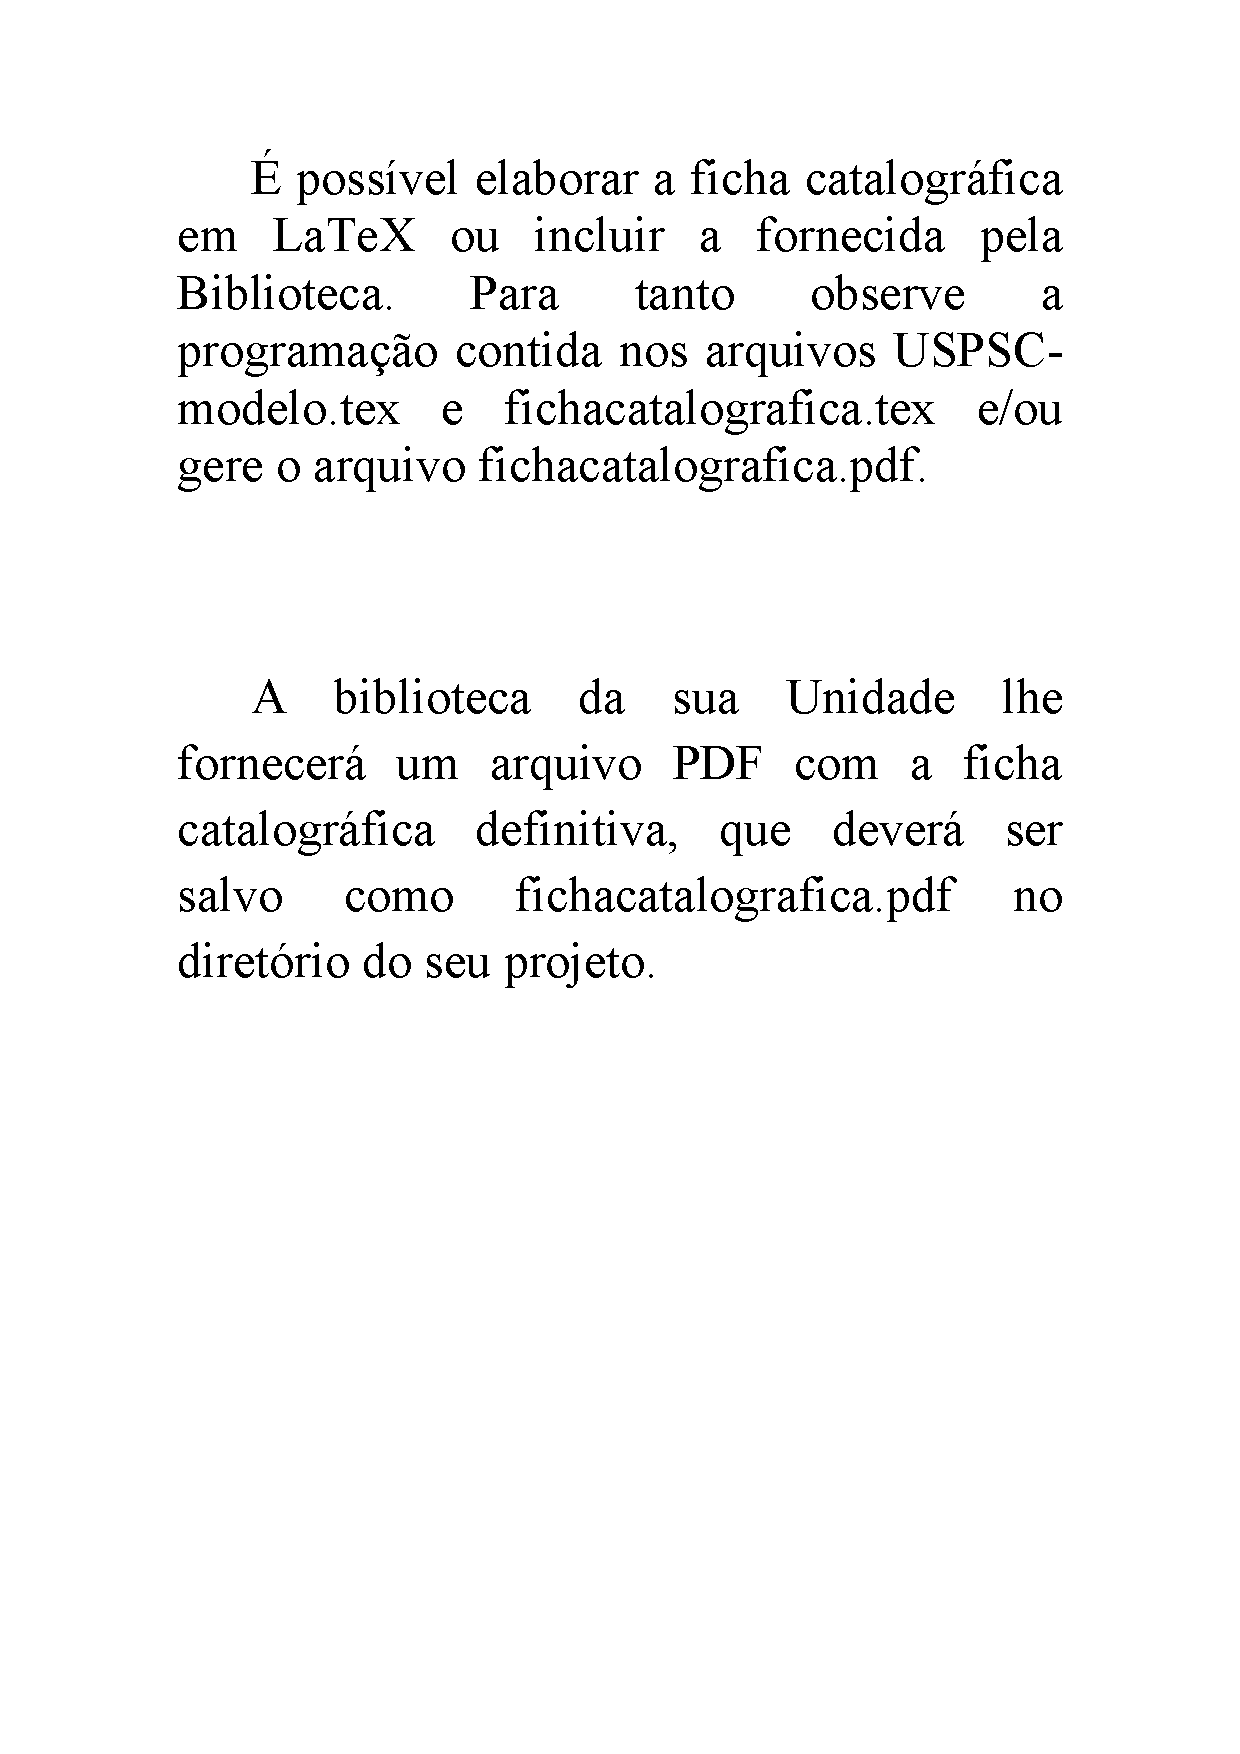
\includepdf{USPSC-TA-PreTextual/USPSC-fichacatalografica.pdf}

% Se você optar por elaborar a ficha catalográfica, deverá 
% incluir uma % antes da linha % antes
% do comando %% USPSC-fichacatalografica.tex
% ---
% Inserir a ficha bibliografica
% ---
% Isto é um exemplo de Ficha Catalográfica, ou ``Dados internacionais de
% catalogação-na-publicação''. Você pode utilizar este modelo como referência. 
% Porém, provavelmente a biblioteca da sua universidade lhe fornecerá um PDF
% com a ficha catalográfica definitiva após a defesa do trabalho. Quando estiver
% com o documento, salve-o como PDF no diretório do seu projeto e substitua todo
% o conteúdo de implementação deste arquivo pelo comando abaixo:
%
\begin{fichacatalografica}
	\hspace{-1.4cm}
	\imprimirnotaautorizacao \\ \\
	%\sffamily
	\vspace*{\fill}					% Posição vertical
\begin{center}					% Minipage Centralizado
  \imprimirnotabib \\
  \begin{table}[htb]
	\scriptsize
	\centering	
	\begin{tabular}{|p{0.9cm} p{8.7cm}|}
		\hline
	      & \\
		  &	  \imprimirautorficha     \\
		
		 \imprimircutter & 
							\hspace{0.4cm}\imprimirtitulo~  / ~\imprimirautor~ ;  ~\imprimirorientadorcorpoficha. -- 	\imprimirlocal, \imprimirdata.   \\
		
		  &  % Para incluir nota referente à versão corrigida no corpo da ficha,
			  % incluir % no início da linha acima e tirar a % do início da linha abaixo
			  %	\hspace{0.4cm} \imprimirtitulo~  / ~\imprimirautor~ ; ~\imprimirorientadorcorpoficha~- ~\imprimirnotafolharosto. -- \imprimirlocal, \imprimirdata.  \\
		
			\hspace{0.4cm}\pageref{LastPage} p. : il. (algumas color.) ; 30 cm.\\ 
		  & \\
		  & 
		    \hspace{0.4cm}\imprimirnotaficha ~--~ 
						  \imprimirunidademin, 
						  \imprimiruniversidademin, 
		                  \imprimirdata. \\ 
		  & \\                 
		   % Para incluir nota referente à versão corrigida em notas,
		    % incluir uma % no início da linha acima e	
		    % tirar a % do início da linha abaixo
		    % & \hspace{0.4cm}\imprimirnotafolharosto \\ 
		  & \\ 
		  & \hspace{0.4cm}1. LaTeX. 2. abnTeX. 3. Classe USPSC. 4. Editoração de texto. 5. Normalização da documentação. 6. Tese. 7. Dissertação. 8. Documentos (elaboração). 9. Documentos eletrônicos. I. \imprimirorientadorficha. 
		   II. Título. \\
	
		     %Se houver co-orientador, inclua % antes da linha (antes de II. Título.) 
		     %          e tire a % antes do comando abaixo 
		     %III. Título. \\   
		  \hline
	\end{tabular}
  \end{table}
\end{center}
\end{fichacatalografica}
% ---

 
% e retirar o % do comando abaixo
%% USPSC-fichacatalograficaTutorial.tex
% ---
% Inserir a ficha bibliografica
% ---
% Isto é um exemplo de Ficha Catalográfica, ou ``Dados internacionais de
% catalogação-na-publicação''. Você pode utilizar este modelo como referência. 
% Porém, provavelmente a biblioteca da sua universidade lhe fornecerá um PDF
% com a ficha catalográfica definitiva após a defesa do trabalho. Quando estiver
% com o documento, salve-o como PDF no diretório do seu projeto e substitua todo
% o conteúdo de implementação deste arquivo pelo comando abaixo:

\textbf{UNIVERSIDADE DE SÃO PAULO} 

Reitor: Vahan Agopyan

Vice-Reitor: Antônio Carlos Hernandes\\

\textbf{Grupo Desenvolvedor do Pacote USPSC} 

\textbf{Coordenação e Programação}

- Marilza Aparecida Rodrigues Tognetti (PUSP-SC)
	
- Ana Paula Aparecida Calabrez (PUSP-SC) 

\textbf{Normalização}

- Ana Paula Aparecida Calabrez (PUSP-SC) 

- Brianda de Oliveira Ordonho Sigolo (IAU)

- Eduardo Graziosi Silva (EESC)

- Eliana de Cássia Aquareli Cordeiro (IQSC)

- Flávia Helena Cassin (EESC)

- Maria Cristina Cavarette Dziabas (IFSC)

- Marilza Aparecida Rodrigues Tognetti (PUSP-SC)

- Regina Célia Vidal Medeiros (ICMC) \\


%
\begin{fichacatalografica}
%	\hspace{-1.4cm}
   \vspace*{\fill}					% Posição vertical
\begin{center}					% Minipage Centralizado
  \imprimirnotabib \\
  \begin{table}[htb]
	\scriptsize
	\centering	
	\begin{tabular}{|p{0.9cm} p{8.7cm}|}
		\hline
	      & \\
		  &	  \imprimirautorficha     \\
		
		 \imprimircutter & 
							\hspace{0.4cm}\imprimirtitulo~ / ~{Marilza Aparecida Rodrigues Tognetti; Ana Paula Aparecida Calabrez,  coordenadoras e progamadoras. Brianda de Oliveira Ordonho Sigolo ...[\textit{et al.}], normalizadoras}.
							 -- 	\imprimirlocal, USP, \imprimirdata.   \\
		
		  &			\hspace{0.4cm}\pageref{LastPage} p. : il. (algumas color.) ; 30 cm.\\ 
 		  & \\ 
		  & \hspace{0.4cm}1. LaTeX. 2. abnTeX. 3. Classe USPSC. 4. Editoração de texto. 5. Normalização da documentação. 6. Tese. 7. Dissertação. 8. Documentos (elaboração). 9. Documentos eletrônicos. I. Calabrez, A. P. A., coord., program., normaliz. II. Sigolo, B. O. O. normaliz. III. Cordeiro, E. C. A., normaliz. IV. Cassin, Flávia Helena, normaliz. V. Dziabas, M. C. C., normaliz. VI. Medeiros, R. C. V., normaliz.  VII. Título.  \\
	
		  \hline
	\end{tabular}
  \end{table}
\end{center}
\end{fichacatalografica}
% ---

% As informações que compõem a ficha catalográfica estão 
% definidas no arquivo USPSC-pre-textual-UUUU.tex
% ---

% ---
% Folha de rosto adicional
% Para imprimir a folha de rosto adicional, exigida por algumas Unidades, a exemplo do ICMC,
% retire a % antes do comando abaixo

%\imprimirfolhaderostoadic

% ---
% ---
% Inserir errata
% ---

%% USPSC-ErrataTutorial.tex
\begin{errata}
	%\OnehalfSpacing 			
	A errata é um elemento opcional, que consiste de uma lista de erros da obra, precedidos pelas folhas e linhas onde eles ocorrem e seguidos pelas correções correspondentes. Deve ser inserida logo após a folha de rosto e conter a referência do trabalho para facilitar sua identificação, conforme a ABNT NBR 14724 \cite{nbr14724}. 
	
    Em USPSC-Tutorial.tex foi utilizado o arquivo \textbf{USPSC-ErrataTutorial.tex}, pois a referência bibliográfica é compatível com o tipo deste documento que é um tutorial (monografia/livro). 
    
    Para teses, dissertações, TCCs e outros trabalhos acadêmicos utilize o arquivo \textbf{USPSC-Errata.tex}, conforme indicado em  USPSC-Modelo.tex e USPSC-TCC-modelo.tex. 
    
       
	Modelo de Errata:
		
	\begin{flushleft} 
			\setlength{\absparsep}{0pt} % ajusta o espaçamento da referência	
			\SingleSpacing 
			\imprimirautorabr.~~\textbf{\imprimirtituloresumo}.~~\imprimirorientador~~	
			%Substitua p. por f. quando utilizar oneside em \documentclass
			%\pageref{LastPage}f.
			\imprimirlocal: \imprimirinstituicao, \imprimirdata. \pageref{LastPage}p. 
 	\end{flushleft}
\vspace{\onelineskip}
\OnehalfSpacing 
\center
\textbf{ERRATA}
\vspace{\onelineskip}
\OnehalfSpacing 
\begin{table}[htb]
	\center
	\footnotesize
	\begin{tabular}{p{2cm} p{2cm} p{4cm} p{4cm} }
		\hline
		\textbf{Folha} & \textbf{Linha}  & \textbf{Onde se lê}  & \textbf{Leia-se}  \\
			\hline
			1 & 10 & auto-conclavo & autoconclavo\\
		\hline
	\end{tabular}
\end{table}
\end{errata}
% ---
%Para Teses, Dissertações, TCCs e outros trabalhos acadêmicos, no arquivo USPSC-Modelo.tex e USPSC-TCC-modelo.tex, utilizar o comando %% USPSC-Errata.tex
\begin{errata}
	%\OnehalfSpacing 			
	A errata é um elemento opcional, que consiste de uma lista de erros da obra, precedidos pelas folhas e linhas onde eles ocorrem e seguidos pelas correções correspondentes. Deve ser inserida logo após a folha de rosto e conter a referência do trabalho para facilitar sua identificação, conforme a ABNT NBR 14724 \cite{nbr14724}.
	
	Modelo de Errata:
		
	\begin{flushleft} 
			\setlength{\absparsep}{0pt} % ajusta o espaçamento da referência	
			\SingleSpacing 
			\imprimirautorabr~ ~\textbf{\imprimirtituloresumo}.	\imprimirdata. \pageref{LastPage}p. 
			%Substitua p. por f. quando utilizar oneside em \documentclass
			%\pageref{LastPage}f.
			\imprimirtipotrabalho~-~\imprimirinstituicao, \imprimirlocal, \imprimirdata. 
 	\end{flushleft}
\vspace{\onelineskip}
\OnehalfSpacing 
\center
\textbf{ERRATA}
\vspace{\onelineskip}
\OnehalfSpacing 
\begin{table}[htb]
	\center
	\footnotesize
	\begin{tabular}{p{2cm} p{2cm} p{4cm} p{4cm} }
		\hline
		\textbf{Folha} & \textbf{Linha}  & \textbf{Onde se lê}  & \textbf{Leia-se}  \\
			\hline
			1 & 10 & auto-conclavo & autoconclavo\\
		\hline
	\end{tabular}
\end{table}
\end{errata}
% ---

% ---

% ---
% Inserir folha de aprovação
% ---

% A Folha de aprovação é um elemento obrigatório da NBR 4724/2011 (seção 4.2.1.3). 
% Após a defesa/aprovação do trabalho, gere o arquivo folhadeaprovacao.pdf da página assinada pela banca 
% e iclua o arquivo utilizando o comando abaixo:
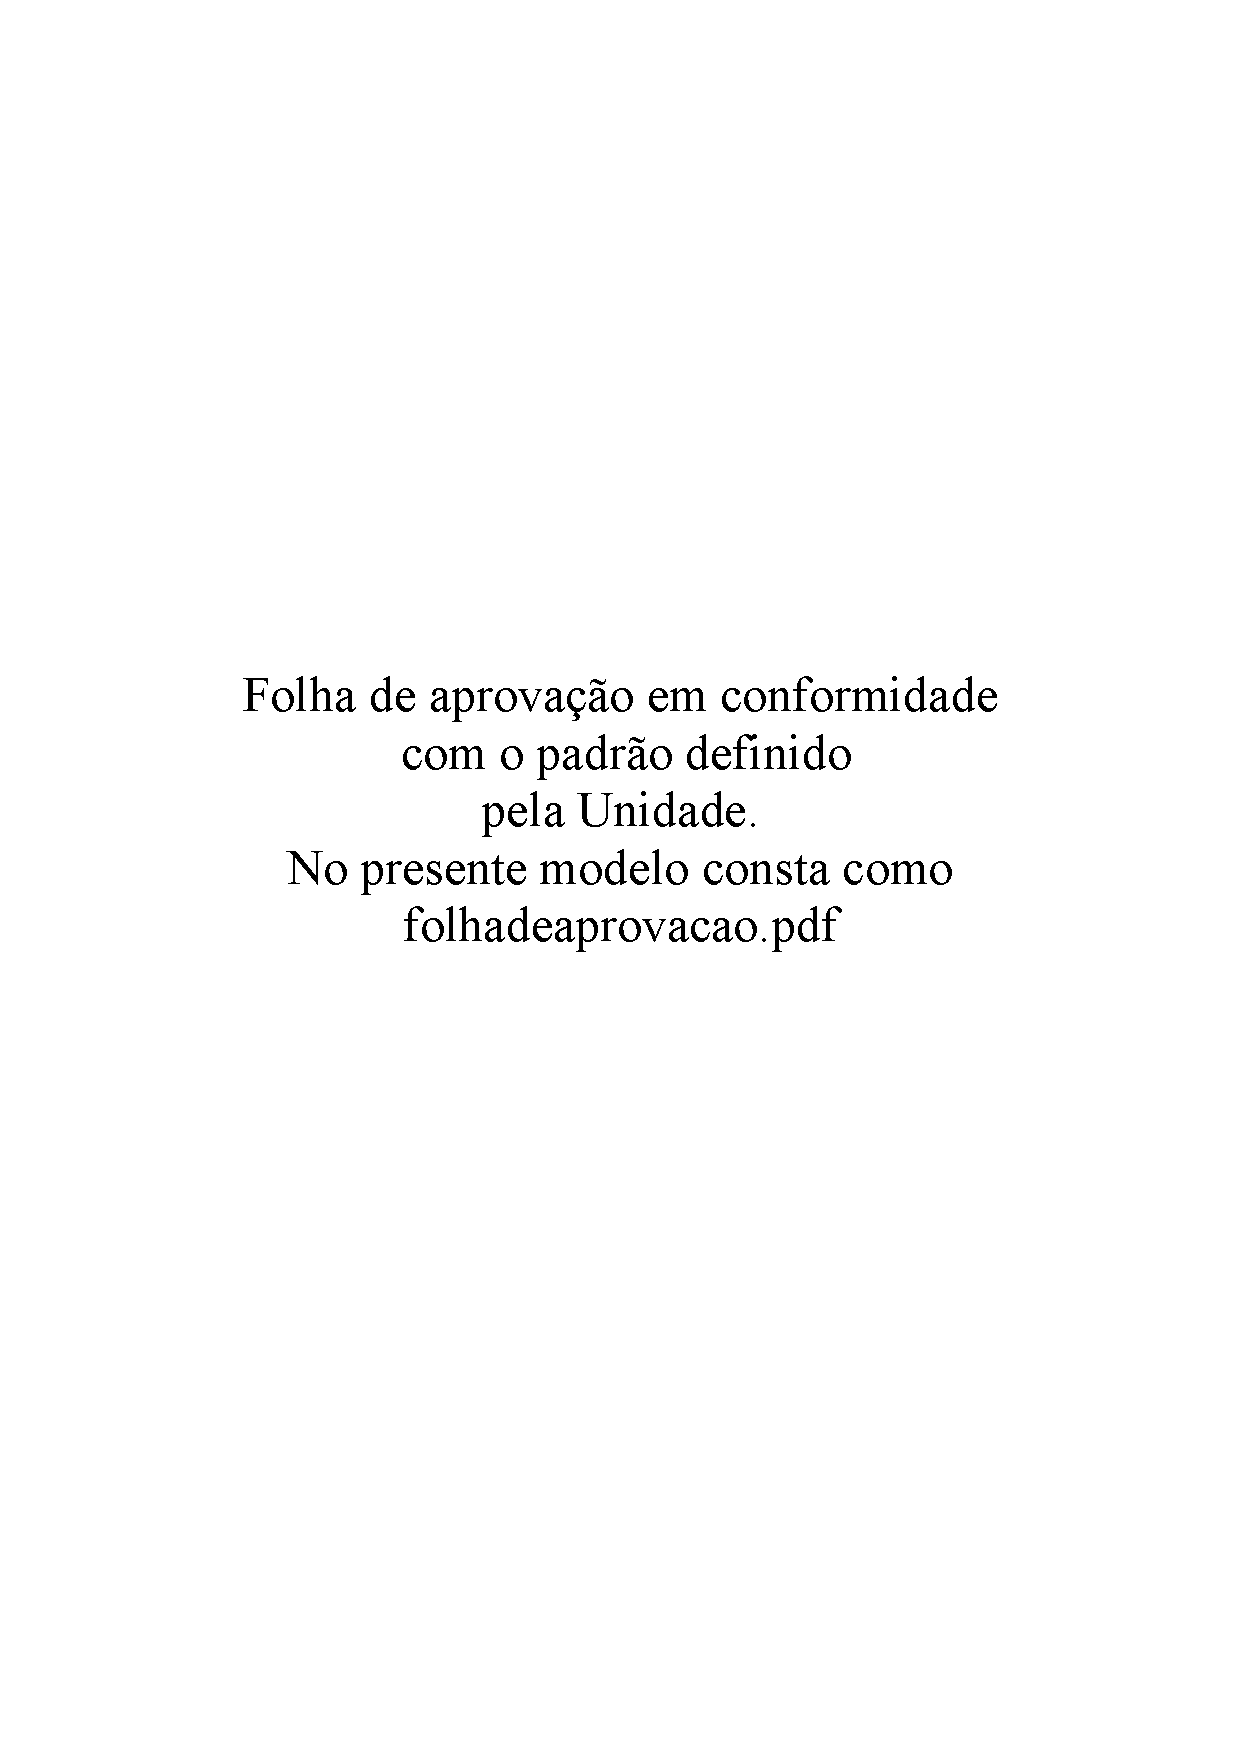
\includepdf{USPSC-TA-PreTextual/USPSC-folhadeaprovacao.pdf}
% Alternativa para a Folha de Aprovação:
% Se for a sua opção elaborar uma folha de aprovação, insira uma % antes do comando acima que inclui o arquivo folhadeaprovacao.pdf,
% tire o % do comando abaixo e altere o arquivo folhadeaprovacao.tex conforme suas necessidades
%\include{folhadeaprovacao}

\includepdf{USPSC-TA-PreTextual/USPSC-PaginaEmBranco.pdf}

% ---
% Dedicatória
% ---
%% USPSC-Dedicatoria.tex
\begin{dedicatoria}
   \vspace*{\fill}
   \centering
   \noindent
   \textit{ Este trabalho é dedicado aos alunos da USP, como uma contribuição\\
  das Bibliotecas do Campus USP de São Carlos para o desenvolvimento\\
	e disseminação da pesquisa científica da Universidade.} \vspace*{\fill}
\end{dedicatoria}
% ---
% ---

% ---
% Agradecimentos
% ---
%% USPSC-AgradecimentosTutorial.tex
\begin{agradecimentos}
	A motivação para o desenvolvimento da classe USPSC e dos modelos de trabalhos acadêmicos foi decorrente de solicitações de usuários das Bibliotecas do Campus USP de São Carlos. A versão 3.0 do Pacote USPSC para modelos de trabalhos acadêmicos é composta da \textbf{Classe USPSC}, do \textbf{Modelo para TCC em \LaTeX\ utilizando o Pacote USPSC} e do \textbf{Modelo para teses e dissertações em \LaTeX\ utilizando o Pacote USPSC}.
	
	Nesta versão do Pacote USPSC, foram feitas alterações na Classe USPSC, inclusão da capa exclusiva para o Instituto de Ciências Matemáticas e de Computação (ICMC), inclusão de novos pacotes e alterações nos modelos de trabalhos acadêmicos.
	
	Na versão 3.0 do Pacote USPSC, as mudanças foram estruturais na programação e conteúdo. Destacamos que os modelos \textbf{USPSC-modelo.tex} e \textbf{USPSC-TCC-modelo.tex} foram simplificados, no que tange ao conteúdo, e foi criado o \textbf{Tutorial do Pacote USPSC para modelos de trabalhos de acad\^emicos em LaTeX - vers\~ao 3.0}, contendo as instruções precisas e detalhadas para melhor utilização dos recursos do Pacote USPSC. Para tanto, foram acrescidos diversos arquivos, para atender as especificidades do tutorial que possui os elementos pré-textuais distintos para teses, dissertações, TCCs e outros trabalhos acadêmicos, conforme descrito em  \textbf{\ref{Pacote} Pacote USPSC: Classe USPSC e modelos de trabalhos de acadêmicos}. A estrutura deste tutorial é igual à  estrutura de trabalhos acadêmicos estabelecida pela ABNT NBR 14724, conforme a \autoref{fig_EstruturaTrabAcad}, portanto o usuário do Pacote USPSC pode utilizar os exemplos e recursos de \LaTeX\ nele contidos.	
	 
	Na versão 3.1 houve a inclusão da capa diferenciada para o Instituto de Ciências Matemáticas e de Computação (ICMC), novos cursos e programas e de algumas alterações na Classe USPSC, arquivos USPSC.cls e  USPSC1.cls.
	
	O Grupo desenvolvedor do Pacote USPSC agradece especialmente ao Luis Olmes, doutorando do ICMC, pelas primeiras orientações sobre o \LaTeX\ . 
	
	Agradecemos ao Lauro César Araujo pelo desenvolvimento da classe  \abnTeX, modelos canônicos e tantas outras contribuições que nos permitiu o desenvolvimento o Pacote USPSC, composto da classe USPSC e seus modelos.
	
	Os nossos agradecimentos aos integrantes do primeiro
	projeto abn\TeX\, Gerald Weber, Miguel Frasson, Leslie H. Watter, Bruno Parente Lima, Flávio de Vasconcellos Corrêa, Otavio Real
	Salvador, Renato Machnievscz, e a todos que contribuíram para que a produção de trabalhos acadêmicos em conformidade com
	as normas ABNT com \LaTeX\ fosse possível.
	
	Agradecemos ao grupo de usuários
	\emph{latex-br}  {\url{http://groups.google.com/group/latex-br}}, aos integrantes do grupo
	\emph{\abnTeX}  {\url{http://groups.google.com/group/abntex2}  e \url{http://www.abntex.net.br/}}~que contribuem para a evolução do \abnTeX.
	
	Agradecemos aos usuários do Pacote USPSC que nos tem dado um \textit{feedback} e sugestões de melhoria. 
	
\end{agradecimentos}
% ---
% ---

% ---
% Epígrafe
% ---
%% USPSC-EpigrafeTutorial.tex
\begin{epigrafe}
    \vspace*{\fill}
	\begin{flushright}
		\textit{``O estudo, a busca da verdade e da beleza são domínios \\
		em que nos é consentido sermos crianças por toda a vida.''\\
		Albert Einstein}
	\end{flushright}
\end{epigrafe}
% ---
% ---

% A T E N Ç Ã O
% Se o idioma do texto for em inglês, o abstract deve preceder o resumo
% resumo em português
%
% Resumo
% ---
%% USPSC-ResumoTutorial.tex
\setlength{\absparsep}{18pt} % ajusta o espaçamento dos parágrafos do resumo		
\begin{resumo}
	\begin{flushleft} 
		\setlength{\absparsep}{0pt} % ajusta o espaçamento da referência	
		\SingleSpacing 
		\imprimirautorabr.~~\textbf{\imprimirtituloresumo}.~~\imprimirorientador~~	
		%Substitua p. por f. quando utilizar oneside em \documentclass
		%\pageref{LastPage}f.
		\imprimirlocal: \imprimirinstituicao, \imprimirdata. \pageref{LastPage}p. 
	\end{flushleft}
\OnehalfSpacing 			
 O resumo deve ressaltar o  objetivo, o método, os resultados e as conclusões do documento. A ordem e a extensão  destes itens dependem do tipo de resumo (informativo ou indicativo) e do  tratamento que cada item recebe no documento original. O resumo deve ser
 precedido da referência do documento, com exceção do resumo inserido no
 próprio documento. (\ldots)  Salientamos que algumas Unidades exigem o titulo dos trabalhos acadêmicos em inglês, tornando necessário a inclusão das referências nos resumos e abstracts, o que foi adotado no \textbf{Modelo para TCC em \LaTeX\ utilizando o Pacote USPSC} e no \textbf{Modelo para teses e dissertações em \LaTeX\ utilizando o Pacote USPSC}. As palavras-chave devem figurar logo abaixo do  resumo, antecedidas da expressão Palavras-chave:, separadas entre si por  ponto e finalizadas também por ponto \cite{nbr6028}.
 

 \textbf{Palavras-chave}: LaTeX. abnTeX. Classe USPSC. Editoração de texto. Normalização da documentação. Trabalho acadêmico. Tese. Dissertação. Trabalho de conclusão de curso (TCC). Documentos (elaboração). Documentos eletrônicos. 
\end{resumo}
% ---

% Abstract
% ---
%% USPSC-AbstractTutorial.tex
%\autor{Silva, M. J.}
\begin{resumo}[Abstract]
 \begin{otherlanguage*}{english}
   \begin{flushleft} 
   	\setlength{\absparsep}{0pt} % ajusta o espaçamento da referência	
   	\SingleSpacing 
   	\imprimirautorabr.~~\textbf{\imprimirtitleabstract}.~~\imprimirorientador~~	
   	%Substitua p. por f. quando utilizar oneside em \documentclass
   	%\pageref{LastPage}f.
   	\imprimirlocal: \imprimirinstituicao, \imprimirdata. \pageref{LastPage}p. 
   \end{flushleft}
	\OnehalfSpacing 
   This is the english abstract.

   \vspace{\onelineskip}
 
   \noindent 
   \textbf{Keywords}: LaTeX. abnTeX. USPSC class. Text editoration. Standardization of documentation. Academic work. Thesis. Dissertation. Conclusion course paper. Documents (development). Electronic documents.
   \end{otherlanguage*}
\end{resumo}

% ---

% ---
% inserir lista de figurass
% ---
\pdfbookmark[0]{\listfigurename}{lof}
\listoffigures*
\cleardoublepage
% ---

% ---
% inserir lista de tabelas
% ---
\pdfbookmark[0]{\listtablename}{lot}
\listoftables*
\cleardoublepage
% ---

% ---
% inserir lista de quadros
% ---
\pdfbookmark[0]{\listofquadroname}{loq}
\listofquadro*
\cleardoublepage
% ---

% ---
% inserir lista de abreviaturas e siglas
% ---
% USPSC-AbreviaturasSiglasTutorial.tex
\begin{siglas}
    \item[ABNT] Associação Brasileira de Normas Técnicas
    \item[abnTeX] ABsurdas Normas para TeX
	\item[EESC] Escola de Engenharia de São Carlos
	\item[IAU] Instituto de Arquitetura e Urbanismo
	\item[IBGE] Instituto Brasileiro de Geografia e Estatística
	\item[ICMC] Instituto de Ciências Matemáticas e de Computação
	\item[IFSC] Instituto de Física de São Carlos
	\item[IQSC] Instituto de Química de São Carlos
	\item[LaTeX] Lamport TeX
	\item[PDF] Portable Document Format
	\item[PUSP-SC] Prefeitura do Campus USP de São Carlos
	\item[TCC] Trabalho de Conclusão de Curso
	\item[USP] Universidade de São Paulo
	\item[USPSC] Campus USP de São Carlos
\end{siglas}

% ---

% ---
% inserir lista de símbolos
% ---
% USPSC-SimbolosTutorial.tex
\begin{simbolos}
  \item[$ \Gamma $] Letra grega Gama
  \item[$ \Lambda $] Lambda
  \item[$ \zeta $] Letra grega minúscula zeta
  \item[$ \in $] Pertence
\end{simbolos}
% ---
% ---
% inserir o sumario
% ---
\pdfbookmark[0]{\contentsname}{toc}
\tableofcontents*
\cleardoublepage
% ---
% ----------------------------------------------------------
% ELEMENTOS TEXTUAIS
% ----------------------------------------------------------
\textual
% Os capítulos são inseridos como arquivos externos 

% Capítulo 1 - Introdução
% ---
%% USPSC-IntroducaoTutorial.tex

% ----------------------------------------------------------
% Introdução (exemplo de capítulo sem numeração, mas presente no Sumário)
% ----------------------------------------------------------
\chapter[Introdução]{Introdução}
\label{Introdução}

Parte inicial do texto, que contém a delimitação do assunto tratado, objetivos da pesquisa e outros elementos necessários para apresentar o tema do trabalho \cite{aguia2020}.

A equipe de desenvolvimento e manutenção do Pacote USPSC, atualmente na versão 3.1, contendo a Classes USPSC, tutorial e modelos para trabalhos acadêmicos em \LaTeX\ utilizando a classe USPSC, foi estabelecida em abril de 2015. É integralmente composta por pessoas vinculadas às Bibliotecas das Unidades de ensino e pesquisa do Campus USP de São Carlos, incluindo a Biblioteca da Prefeitura do Campus USP de São Carlos (PUSP-SC), para garantir a sustentabilidade deste produto, tendo autonomia para implementar novos recursos, efetuar compatibilizações necessárias em decorrência de alterações de normas da ABNT e/ou normas e padrões estabelecidos pelas comissões de pós-graduação das Unidades, incluir novos programas de pós-graduação das Unidades, dentre outras razões.

O Grupo Desenvolvedor do Pacote USPSC optou por manter os exemplos apresentados nas versões anteriores do tutorial, que são os relacionados no capítulo \textbf{\ref{Referências} MODELOS DE REFERÊNCIAS} do documento \textbf{Diretrizes para apresentação de dissertações e teses da USP}: documento eletrônico e impresso - Parte I (ABNT), 3ª edição de 2016, porém em conformidade com ABNT NBR 6023:2018. 

Atualmente a USP em São Carlos possui a Prefeitura do Campus USP de São Carlos (PUSP-SC), o Centro de Divulgação Científica e Cultural (CDCC) e as seguintes Unidades de ensino e pesquisa: Escola de Engenharia de São Carlos (EESC), Instituto de Ciências Matemáticas e de Computação (ICMC), Instituto de Física de São Carlos (IFSC), Instituto de Química de São Carlos (IQSC) e o Instituto de Arquitetura e Urbanismo (IAU)).

Na versão 2.0 o Pacote USPSC passou a ser composto pela \textbf{Classe USPSC}, o \textbf{Modelo para TCC em \LaTeX\ utilizando a classe USPSC} e o \textbf{Modelo para teses e dissertações em \LaTeX\ utilizando a classe USPSC} para a EESC.

Na versão 3.0 do Pacote USPSC os modelos de trabalhos acadêmicos \textbf{USPSC-modelo.tex} e \textbf{USPSC-TCC-modelo.tex} foram simplificados, no que tange ao conteúdo, e foi criado o \textbf{Tutorial do Pacote USPSC para modelos de trabalhos de acad\^emicos em LaTeX - vers\~ao 3.0}, contendo as instruções precisas e detalhadas para melhor utilização dos recursos do Pacote USPSC. Para tanto, foram acrescidos diversos arquivos, para atender as especificidades do tutorial que possui os elementos pré-textuais distintos para teses, dissertações, TCCs e outros trabalhos acadêmicos, conforme descrito em  \textbf{\ref{Pacote} Pacote USPSC: Classe USPSC e modelos de trabalhos de acadêmicos}. A estrutura deste tutorial é igual à  estrutura de trabalhos acadêmicos estabelecida pela ABNT NBR 14724, conforme a \autoref{fig_EstruturaTrabAcad}.		

A versão 3.0 do Pacote USPSC traz ainda as seguintes alterações e implementações:

\begin{alineas}	 
	\item foi alterada a estrutura da pasta para distribuir mais didaticamente os diversos arquivos que compõem o referido pacote, conforme descrito em \ref{Pacote}; 
	\item foram criados os seguintes arquivos de elementos pré-textuais: USPSC-Errata.tex, USPSC-Dedicatoria.tex, USPSC-Agradecimentos.tex, USPSC-Epigrafe.tex,\\
	USPSC-Resumo.tex, USPSC-Abstract.tex, USPSC-AbreviaturasSiglas.tex e USPSC-Simbolos.tex. 
	Tais informações constavam diretamente dos arquivos \textbf{USPSC-modelo.tex} e  \textbf{USPSC-TCC-modelo.tex} e nesta versão passaram a ser incluídas através do comando \verb+\include{nome do arquivo tex}+;
	\item implementação do Modelo para TCC para o ICMC e IQSC, conforme descrito em \ref{Pacote};
	\item alteração do pacote utilizado para estruturas, reações e mecanismos de reações químicas, conforme descrito em \ref{Reaquimica};
	\item alterações na Classe USPSC (USPSC.cls e USPSC1.cls):
		\begin{subalineas}
			\item foi adicionado o comando \verb+\ABNTEXcaptiondelim+ e alterado o separador de \textbf{captions} para \textbf{long dash} visando a compatibilização com a norma  ABNT NBR 14724:2011 e a conformidade com a classe \abnTeX\ v1.9.6;
			\item para incluir novos comandos e parâmetros para possibilitar a impressão de página de rosto adicional, atualmente adotada apenas pelo ICMC;
		\end{subalineas}
	\item alterações no arquivo USPSC-pre-textual-EESC.tex em decorrência das alterações nos programas de pós-graduação;
	\item alterações no arquivo USPSC-pre-textual-IFSC.tex para incluir opções de programas em inglês;
	\item alterações no arquivo USPSC-pre-textual-ICMC.tex para incluir os comandos e parâmetros referentes à página de rosto adicional;
	\item alterações no arquivo USPSC-Unidades.tex para incluir os comandos relativos aos novos Modelos de TCC;
	\item criação dos arquivos USPSC-TCC-pre-textual-ICMC.tex e USPSC-TCC-pre-textual-IQSC.tex, necessários para implementar o Modelo para TCC para o ICMC e IQSC;
	\item alteração no capítulo \textbf{\ref{Referências} MODELOS DE REFERÊNCIAS}, mantendo os exemplos contidos nas \textbf{Diretrizes para apresentação de dissertações e teses da USP}: documento eletrônico e impresso - Parte I (ABNT), porém em conformidade com ABNT NBR 6023:2018; 
	\item inclusão da alternativa de cores para os links nos arquivos \textbf{USPSC-modelo.tex} e \textbf{USPSC-TCC-modelo.tex}, conforme descrito em \ref{coreslinks} 
	\item alterações no arquivo \textbf{USPSC-modelo.tex} e nos demais arquivos \textbf{.tex} em conformidade com as alterações e implementações efetuadas.	\\
\end{alineas}

	A versão 3.1 traz as alterações na Classe USPSC (USPSC.cls e USPSC1.cls) específicas para incluir novos parâmetros para capa e tipo de publicação em inglês.

	O Grupo Desenvolvedor do Pacote USPSC está assim constituído:

\textbf{Coordenação e Programação}

- Marilza Aparecida Rodrigues Tognetti - marilza@sc.usp.br (PUSP-SC)	

- Ana Paula Aparecida Calabrez - aninha@sc.usp.br (PUSP-SC) 

\textbf{Normalização e Padronização}

- Ana Paula Aparecida Calabrez - aninha@sc.usp.br (PUSP-SC)

- Brianda de Oliveira Ordonho Sigolo - brianda@usp.br (IAU)

- Eduardo Graziosi Silva - edu.gs@sc.usp.br (EESC)

- Eliana de Cássia Aquareli Cordeiro - eliana@iqsc.usp.br (IQSC)

- Flávia Helena Cassin - cassinp@sc.usp.br (EESC)	

- Maria Cristina Cavarette Dziabas - mcdziaba@ifsc.usp.br (IFSC)	

- Marilza Aparecida Rodrigues Tognetti - marilza@sc.usp.br (PUSP-SC)

- Regina Célia Vidal Medeiros - rcvm@icmc.usp.br (ICMC)

	O objetivo do presente trabalho é apresentar a versão 3.1 do Pacote USPSC, composto pela \textbf{Classe USPSC}, \textbf{Tutorial do Pacote USPSC para modelos de trabalhos de acad\^emicos em LaTeX - vers\~ao 3.1},  \textbf{Modelo para TCC em \LaTeX\ utilizando a classe USPSC} e o \textbf{Modelo para teses e dissertações em \LaTeX\ utilizando a classe USPSC}, concebidos em conformidade com a \textbf{ABNT NBR 14724} \cite{nbr14724}, as \textbf{Diretrizes para apresentação de dissertações e teses da USP} \cite{aguia2020} e normas e padrões estabelecidos pelas Unidades. 
	
	A expectativa é que o Pacote USPSC, mediante os modelos propostos, proporcione o aprimoramento da qualidade dos trabalhos acadêmicos produzidos pelos alunos de graduação e de pós-graduação das referidas Unidades de Ensino e Pesquisa do Campus USP de São Carlos, garantindo a normalização e padronização estabelecidas.
	
	
% ---

% ---
% Capítulo 2
% ---
%% USPSC-Cap2-DesenvolvimentoTutorial.tex 

% ---
% Este capítulo, utilizado por diferentes exemplos do abnTeX2, ilustra o uso de
% comandos do abnTeX2 e de LaTeX.
% ---

\chapter{Desenvolvimento}\label{cap_exemplos}
Este capítulo é parte principal do trabalho acadêmico e deve conter a exposição ordenada e detalhada do assunto. Divide-se em seções e subseções, em conformidade com a abordagem do tema e do método, abrangendo: revisão bibliográfica, materiais e métodos, técnicas utilizadas, resultados obtidos e discussão.

O conteúdo deste documento visa apresentar um tutorial para utilização do Pacote USPSC, composto da Classe USPSC, tutorial e modelos, utilizando a estrutura de trabalhos acadêmicos, mas por questões didáticas adotou-se capítulo, seções e subseções diferentes das usualmente utilizadas.


\section{Pacote USPSC: Classe USPSC e modelos de trabalhos acadêmicos}\label{Pacote}
A versão 3.1 do Pacote USPSC traz os modelos simplificados de trabalhos acadêmicos \textbf{USPSC-modelo.tex} e \textbf{USPSC-TCC-modelo.tex} e o \textbf{Tutorial do Pacote USPSC para modelos de trabalhos acad\^emicos em LaTeX - vers\~ao 3.1}, contendo as instruções precisas e detalhadas para melhor utilização dos recursos do Pacote USPSC. Para tanto, foram acrescidos diversos arquivos, para atender as especificidades do tutorial que possui os elementos pré-textuais distintos para teses, dissertações, TCCs e outros trabalhos acadêmicos, conforme descrito em  \textbf{\ref{Pacote} Pacote USPSC: Classe USPSC e modelos de trabalhos acadêmicos}. A estrutura deste tutorial é igual à estrutura de trabalhos acadêmicos estabelecida pela ABNT NBR 14724, conforme a \autoref{fig_EstruturaTrabAcad}.

Todas as alterações e novas implementações foram relacionadas em \textbf{\ref{Introdução} INTRODUÇÃO} e neste capítulo serão descritas detalhadamente, quando necessário. 

A classe USPSC é uma derivada da classe \textbf{\abnTeX\ v1.9.5} para as Unidades de ensino e pesquisa do Campus USP de São Carlos:
Escola de Engenharia de São Carlos (EESC), Instituto de Arquitetura e Urbanismo (IAU), Instituto de Ciências Matemáticas e de Computação (ICMC), Instituto de Física de São Carlos (IFSC) e Instituto de Química de São Carlos (IQSC).

O objetivo do projeto é disponibilizar modelos em \LaTeX\  para a elaboração de trabalhos acadêmicos (tese, dissertação, trabalho de conclusão de curso (TCC), dentre outros) em conformidade com a \textbf{ABNT NBR 14724}: informação e documentação: trabalhos acadêmicos: apresentação \cite{nbr14724}, \textbf{Diretrizes para apresentação de dissertações e teses da USP}: documento eletrônico e impresso - Parte I (ABNT) \cite{aguia2020} e normas e padrões estabelecidos pelas Unidades.

Este documento e seu código fonte são exemplos de uso da \textbf{Classe USPSC} e do pacote \textbf{abntex2cite}.
Para complementar as instruções contidas neste documento, utilize os manuais \cite{abnetxclasse,abnetxcite,abnetxcitealf} e da classe \textsf{memoir}\cite{memoir2010}. 


Os referidos modelos seguem a estrutura de trabalhos acadêmicos estabelecida pela ABNT NBR 14724, conforme a \autoref{fig_EstruturaTrabAcad}. 

\begin{figure}[htb]
	\caption{\label{fig_EstruturaTrabAcad}Estrutura do trabalho acadêmico}
	\begin{center}
		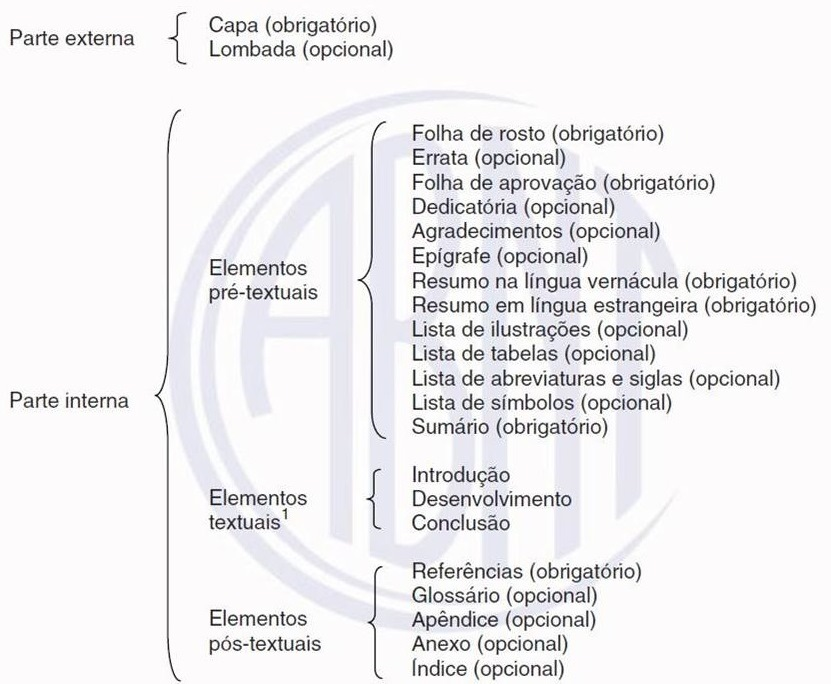
\includegraphics[scale=0.5]{USPSC-img/USPSC-EstruturaTrabAcad.jpg}
	\end{center}
	\legend{Fonte: \citeonline{nbr14724}}
\end{figure}

A versão v.3.1 do Pacote USPSC, por \textit{default}, é instalado em uma pasta denominada USPSC-v3.1 com a seguinte distribuição dos arquivos utilizados para gerar o documento em formato PDF, mediante a compilação utilizando um dos editores \LaTeX\ :


\begin{alineas}	
	\item \verb+ ...\USPSC-v3.1\ + contendo:	
		\begin{alineas}
			\item arquivo principal do tutorial: USPSC-tutorial.tex;
			\item arquivos principais do modelo para teses e dissertações:
				\begin{subalineas}
					\item USPSC-modelo.tex;
					\item USPSC-modelo-EESC.tex;
					\item USPSC-modelo-IAU.tex;
					\item USPSC-modelo-ICMCe.tex (idioma do texto em inglês);
					\item USPSC-modelo-ICMCp.tex (idioma do texto em português);
					\item USPSC-modelo-IFSCe.tex (idioma do texto em inglês);
					\item USPSC-modelo-IFSCp.tex (idioma do texto em português);
					\item USPSC-modelo-IQSC.tex;
				\end{subalineas}
			\item arquivos principais do modelo para TCC: 
			\begin{subalineas}
				\item USPSC-TCC-modelo.tex;
				\item USPSC-TCC-modelo-EESC.tex;
				\item USPSC-TCC-modelo-ICMCe.tex (idioma do texto em inglês);
				\item USPSC-TCC-modelo-ICMCp.tex (idioma do texto em português);
				\item USPSC-TCC-modelo-IQSC.tex;
			\end{subalineas}
			\item arquivo que relaciona os arquivos pré-textuais dos programas de Pós-Graduação e TCCs das Unidades: USPSC-unidades.tex;
			\item arquivos pré-textuais: USPSC-pre-textual-UUUU.tex e USPSC-TCC-pre-textual-UUUU.tex;
			\item pastas especificadas nos itens abaixo;
	   	\end{alineas}
	   	
	\item \verb+ ...\USPSC-v3.1\USPSC-bib\ + com o arquivo de dados das citações e referências utilizadas: 
		\begin{alineas}	
			\item USPSC-modelo-references.bib;
		\end{alineas} 
		
	\item \verb+ ...\USPSC-v3.1\USPSC-classe\ + com os arquivos da classe USPSC, incluindo os referentes à compatibilização com a ABNT NBR 6023:2018:
		\begin{alineas}
			\item USPSC.cls;
			\item USPSC1.cls; 
			\item arquivo ABNT6023-2018.sty, para tirar <> da URL, chamado mediante o comando  \verb+ \usepackage{USPSC-classe/ABNT6023-2018}+;
			\item as demais compatibilizações estão nos arquivos abntex2-alf-USPSC.bst, abntex2-alfeng-USPSC.bst, abntex2-num-USPSC.bst e abntex2-numeng-USPSC.bst, chamados através do comando \newline \verb+\bibliographystyle{USPSC-classe/abntex2-alf-USPSC} + ou \newline
			\verb+\bibliographystyle{USPSC-classe/abntex2-alfeng-USPSC} + ou \newline
			\verb+\bibliographystyle{USPSC-classe/abntex2-num-USPSC}+ ou \newline \verb+\bibliographystyle{USPSC-classe/abntex2-numeng-USPSC}+, dependendo se o Sistemas de chamada for autor-data ou numérico; 
		\end{alineas}	
	    
	\item \verb+ ...\USPSC-v3.1\USPSC-Tutorial\ + contendo:
		\begin{subalineas}
			\item USPSC-fichacatalograficaTutorial.tex;
			\item USPSC-ErrataTutorial.tex;
			\item USPSC-DedicatoriaTutorial.tex;
			\item USPSC-AgradecimentosTutorial.tex;
			\item USPSC-EpigrafeTutorial.tex;
			\item USPSC-ResumoTutorial.tex;
			\item USPSC-AbstractTutorial.tex;
			\item USPSC-AbreviaturasSiglasTutorial.tex;
			\item USPSC-SimbolosTutorial.tex;
			\item USPSC-Cap1-IntroducaoTutorial.tex;
			\item USPSC-Cap2-DesenvolvimentoTutorial;
			\item USPSC-Cap3-CitacoesTutorial.tex;
			\item USPSC-Cap4-ReferenciasTutorial.tex;
			\item USPSC-Cap5-ConclusaoTutorial.tex;
			\item USPSC-ApendicesTutorial.tex;
			\item USPSC-AnexosTutorial.tex;
			\item USPSC-IndicesRemissivosTutorial.tex.
		\end{subalineas}
	
	\item \verb+ ...\USPSC-v3.1\USPSC-TA-PreTextual\ + com os arquivos relativos aos elementos pré-textuais de trabalhos acadêmicos:
		\begin{alineas}
				\item USPSC-CapaICMC.tex;
				\item USPSC-fichacatalografica.tex;
				\item USPSC-fichacatalografica.pdf;
				\item USPSC-folhadeaprovacao.tex;
				\item USPSC-folhadeaprovacao.pdf;
				\item USPSC-Errata.tex;
				\item USPSC-Dedicatoria.tex;
				\item USPSC-Agradecimentos.tex;
				\item USPSC-Epigrafe.tex;
				\item USPSC-Resumo.tex;
				\item USPSC-Abstract.tex;
				\item USPSC-AbreviaturasSiglas.tex
				\item USPSC-Simbolos.tex 
				\item USPSC-PaginaEmBranco.pdf
			\end{alineas}
			
	\item \verb+ ...\USPSC-v3.1\USPSC-TA-Textual\ + contendo os arquivos relativos aos elementos textuais de trabalhos acadêmicos:
		\begin{alineas}
			\item USPSC-Cap1-Introducao.tex;
			\item USPSC-Cap2-Desenvolvimento.tex;
			\item USPSC-Cap3-Conclusao.tex;
		\end{alineas}
		
	\item \verb+ ...\USPSC-v3.1\USPSC-TA-PosTextual\ + para os arquivos relativos aos elementos pós-textuais de trabalhos acadêmicos:	
		\begin{alineas}
			\item USPSC-Apendices.tex;
			\item USPSC-Anexos.tex;
			\item USPSC-IndicesRemissivos.tex;
		\end{alineas}
	
	\item \verb+ ...\USPSC-v3.1\USPSC-img\ + contendo os arquivos de imagens e os PDFs relacionados no texto dos modelos: 
		\begin{alineas}	
			\item USPSC-AcentuacaoLaTeX.png;
			\item CapaICMC.jpg;
			\item USPSC-EstruturaTrabAcad.jpg;
			\item USPSC-LetrasGregas.png;
			\item USPSC-modelo-img-grafico.pdf;
			\item USPSC-modelo-img-marca.pdf;
			\item USPSC-SimbolosUteis.png;
		\end{alineas}	
	
	\item \verb+ ...\USPSC-v3.1\USPSC-Siglas\ + traz os arquivos que relacionam as siglas das Unidades e as definidas para os cursos de graduação e programas de pós-graduação, que não necessariamente são as oficiais utilizadas pela Universidade: 
		\begin{alineas}	
			\item USPSC-Siglas estabelecidas para os Programas de Pós-Graduação por Unidade.xlsx;
			\item USPSC-TCC-Siglas estabelecidas para as Graduações por Unidade.xlsx;
		\end{alineas}
		
	\item \verb+ ...\USPSC-v3.1\USPSC-Sobre\ + contém arquivos sobre cada versão do Pacote USPSC.

\end{alineas}	 

		
Para tese ou dissertação deverá ser utilizado o arquivo USPSC-modelo.tex, onde o autor deverá indicar a sigla da Unidade e a sigla do programa de pós-graduação que está vinculado, a exemplo dos comandos abaixo:
		
			\begin{verbatim}
				\siglaunidade{IQSC}
				\programa{MQOB}
			\end{verbatim}
			
Para o \textbf{Modelo para teses e dissertações em \LaTeX\ utilizando o Pacote USPSC} estão definidos os seguintes arquivos pré-textuais:
			
			\begin{alineas}	 
				\item USPSC-pre-textual-EESC.tex;
				\item USPSC-pre-textual-IAU.tex;
				\item USPSC-pre-textual-ICMC.tex;
				\item USPSC-pre-textual-IFSC.tex;
				\item USPSC-pre-textual-IQSC.tex.
			\end{alineas}
			
Para TCC deverá ser utilizado o arquivo USPSC-TCC-modelo.tex, onde o autor deverá indicar a \textbf{'sigla da Unidade'} + \textbf{'-TCC'} (Exemplo: EESC-TCC) e a sigla do curso de graduação que está vinculado, a exemplo dos comandos abaixo:
			
			\begin{verbatim}
			\siglaunidade{EESC-TCC}
			\programa{EAMB}
			\end{verbatim}
			
Atualmente estão disponíveis os dados pré-textuais para a EESC, ICMC e IQSC:
			
			\begin{alineas}	 
				\item USPSC-TCC-pre-textual-EESC.tex;
				\item USPSC-TCC-pre-textual-ICMC.tex;
				\item USPSC-TCC-pre-textual-IQSC.tex.
			\end{alineas}
			
Serão incluídos os demais arquivos quando as demais Unidades do Campus USP de São Carlos estabelecerem seus padrões. 
			
Para utilizar corretamente os dados pré-textuais, é necessário consultar as siglas estabelecidas para os cursos de graduação e para os programas de pós-graduação da Unidade de vínculo nos quadros dos \textbf{APÊNDICES B-I} ou nas planilhas \textbf{USPSC-TCC-Siglas estabelecidas para as Graduações por Unidade.xlsx} e \textbf{USPSC-Siglas estabelecidas para os programas de pós-graduação por Unidade.xlsx}. 

Os arquivos com dados pre-textuais estão nominados como USPSC-pre-textual-UUUU.tex ou USPSC-TCC-pre-textual-UUUU.tex, onde UUUU é a sigla da Unidade. Inicialmente estão disponibilizados apenas os pré-textuais das Unidades do Campus USP de São Carlos.
			
Foram definidos os arquivos USPSC-pre-textual-OUTRO.tex e USPSC-TCC-pre-textual-OUTRO.tex que serão executados quando uma das siglas for diferente das explicitadas para as Unidades e/ou para os cursos de graduação e/ou para os programas de Pós-Graduação. O preâmbulo será incompleto e apresentando "..." no final, evidenciando que o autor deverá rever as siglas utilizadas.

Através do comando \verb+ %% USPSC-unidades.tex
% Camando para definição do programa de Pós-Graduação, Especialidade do Título e Instituição
\newcommand{\siglaunidade}[1]{


% EESC-TCC ==========================================================================
    \ifthenelse{\equal{#1}{EESC-TCC}}{
     			\include{USPSC-TCC-pre-textual-EESC}
% ---
    }{
% EESC ==========================================================================
	\ifthenelse{\equal{#1}{EESC}}{
	\include{USPSC-pre-textual-EESC}
	% ---
}{    
% IAU ===========================================================================
        \ifthenelse{\equal{#1}{IAU}}{
        \include{USPSC-pre-textual-IAU}    
        }{
% ICMC ===========================================================================
        \ifthenelse{\equal{#1}{ICMC}}{
        %% USPSC-pre-textual-ICMC.tex
%% Camandos para definição do tipo de documento (tese ou dissertação ou monografia), área de concentração, opção, preâmbulo, titulação 
%% referentes ao Programa de Pós-Graduação o ICMC
\instituicao{Instituto de Ci\^encias Matem\'aticas e de Computa\c{c}\~ao, Universidade de S\~ao Paulo}
\unidade{INSTITUTO DE CI\^ENCIAS MATEM\'ATICAS E DE COMPUTA\c{C}\~AO}
\unidademin{Instituto de Ci\^encias Matem\'aticas e de Computa\c{c}\~ao}
\universidademin{Universidade de S\~ao Paulo}
\setorpos{SERVI\c{C}O DE P\'OS-GRADUA\c{C}\~AO DO ICMC-USP}

\notafolharosto{Vers\~ao original}
\notafolharostoadic{Original version}
%Para versão original em inglês, comente os comandos/declarações acima (inclua % antes do comando acima) 
% e tire a % dos comandos/declarações abaixo no idioma do texto
%\notafolharosto{Original version}
%\notafolharostoadic{Vers\~ao original}
 
%Para versão revisada, comente os comandos/declarações acima (inclua % antes do comando acima) 
% e tire a % dos comandos/declarações abaixo, em conformidade com o idioma do texto
% Se o Idioma do texto for português: 
%\notafolharosto{Vers\~ao revisada}
%\notafolharosto{Final version}
% Se o Idioma do texto for Inglês: 
%\notafolharosto{Final version}
%\notafolharosto{Vers\~ao revisada}
% ---
% dados complementares para CAPA e FOLHA DE ROSTO
% ---
\universidade{UNIVERSIDADE DE S\~AO PAULO}

% Idioma do texto em PORTUGUÊS
\titulo{Metodologia para prever a reinternação hospitalar de pacientes baseada em Inteligência Artificial Explicável}
\titleabstract{Methodology for Predicting Hospital Readmission of Patients Based on Explainable Artificial Intelligence}
\tituloadic{Methodology for Predicting Hospital Readmission of Patients Based on Explainable Artificial Intelligence}
\tituloresumo{Metodologia para prever a reinternação hospitalar de pacientes baseada em Inteligência Artificial Explicável}

% Idioma do texto em INGLÊS
% 22/02/2017 - Título para página de rosto adicional
% para a versão em inglês, utilize os comandos abaixo, e inclua % no início dos 4 comandos logo acima,  cada comando acima que são referentes ao texto do Trabalho Acadêmico em português
%\titulo{Model for thesis and dissertations in LaTeX using the USPSC Package to the ICMC}
%\titleabstract{Model for thesis and dissertations in LaTeX using the USPSC Package to the ICMC}
%\tituloadic{Modelo para teses e disserta\c{c}\~oes em LaTeX utilizando o Pacote USPSC para o ICMC}
%\tituloresumo{Modelo para teses e disserta\c{c}\~oes em LaTeX utilizando o Pacote USPSC para o ICMC}

\autor{Matheus Mendes dos Santos}
\autorficha{Santos, Matheus Mendes dos}
\autorabr{SANTOS, MENDES M.}

% \cutter{S856m}
% Para gerar a ficha catalográfica sem o Código Cutter, basta 
% incluir uma % na linha acima e tirar a % da linha abaixo
\cutter{ }

\local{S\~ao Carlos}
\data{2023}

% Para o idioma português:
\renewcommand{\orientadorname}{Orientador:}
\orientador{Prof. Dr. Rodrigo Colnago Contreras}
\orientadoradic{Advisor: Prof. Dr. Rodrigo Colnago Contreras}
\orientadorcorpoficha{orientador Rodrigo Colnago Contreras}
\orientadorficha{Contreras, R. C, orient}
%Para incluir o nome do(a) coorientados(a), inclua % nos 2 comandos acima e retire a % dos 2 comandos abaixo
%\orientadorcorpoficha{orientadora Elisa Gon\c{c}alves Rodrigues ;  co-orientador Jo\~ao Alves Serqueira}
%\orientadorficha{Rodrigues, Elisa Gon\c{c}alves, orient. II. Serqueira, Jo\~ao Alves, co-orient}


%Se o idoma for o inglês, inclua % nos comandos acima e exclua dos comandos abaixo
%\renewcommand{\orientadorname}{Advisor:}
%\orientador{Profa. Dra. Elisa Gon\c{c}alves Rodrigues}
%\orientadoradic{Orientadora: Profa. Dra. Elisa Gon\c{c}alves Rodrigues}
%\orientadorcorpoficha{orientadora Elisa Gon\c{c}alves Rodrigues}
%\orientadorficha{Rodrigues, Elisa Gon\c{c}alves, orient}
%Para incluir o nome do(a) coorientados(a), inclua % nos 2 comandos acima e retire a % dos 2 comandos abaixo
%\orientadorcorpoficha{orientadora Elisa Gon\c{c}alves Rodrigues ;  co-orientador Jo\~ao Alves Serqueira}
%\orientadorficha{Rodrigues, Elisa Gon\c{c}alves, orient. II. Serqueira, Jo\~ao Alves, co-orient}

% Quando houver Coorientador(a): 
% Para o idioma português:
% basta retirar  % antes de um dos comandos abaixo
%\newcommand{\coorientadorname}{Coorientador:}
%\newcommand{\coorientadorname}{Coorientadora:}
% Para o idoma inglês:
% basta retirar  % antes do comando abaixo
%\newcommand{\coorientadorname}{Coorientador:}

% Quando houver Coorientador(a), basta tirar a % utilizar o comando abaixo
%\newcommand{\coorientadorname}{Coadvisor:}
%Se houver co-orientador, inclua % antes das duas linhas (antes dos comandos \orientadorcorpoficha e \orientadorficha) 
%          e tire a % antes dos 3 comandos abaixo
%\coorientador{Prof. Dr. Jo\~ao Alves Serqueira}
%\coorientadoradic{ Co-orientador: Prof. Dr. Jo\~ao Alves Serqueira}
%\orientadorcorpoficha{orientadora Elisa Gon\c{c}alves Rodrigues ;  co-orientador Jo\~ao Alves Serqueira}
%\orientadorficha{Rodrigues, Elisa Gon\c{c}alves, orient. II. Serqueira, Jo\~ao Alves, co-orient}

%Para o idioma Inglês, retire a % antes da linha abaixo
%\renewcommand{\areaname}{Concentration area: }

		
\notaautorizacao{AUTORIZO A REPRODU\c{C}\~AO E DIVULGA\c{C}\~AO TOTAL OU PARCIAL DESTE TRABALHO, POR QUALQUER MEIO CONVENCIONAL OU ELETR\^ONICO PARA FINS DE ESTUDO E PESQUISA, DESDE QUE CITADA A FONTE.}
% Se o idioma for o inglês, inclua a % antes do campo \notaautorizacao acima e retire a % da linha abaixo
%\notaautorizacao{I AUTORIZE THE REPRODUCTION AND DISSEMINATION OF TOTAL OR PARTIAL COPIES OF THIS DOCUMENT, BY CONVENCIONAL OR ELECTRONIC MEDIA FOR STUDY OR RESEARCH PURPOSE, SINCE IT IS REFERENCED.}

\notabib{Ficha catalogr\'afica elaborada pela Biblioteca Prof. Achille Bassi, ICMC/USP, com os dados fornecidos pelo(a) autor(a)}

\newcommand{\programa}[1]{
% MPMp ==========================================================================
\ifthenelse{\equal{#1}{MPMp}}{
	\tipotrabalho{Disserta\c{c}\~ao (Mestrado em Ci\^encias)}
	\tipotrabalhoabs{Dissertation (Master in Science)}
	\area{Matem\'atica em Rede Nacional}
	\areaadic{Concentration area: Mathematics in National Network}
	%\opcao{Nome da Opção em português}
	%\opcaoadic{Nome da Opção em inglês}
	% O preambulo deve conter o tipo do trabalho, o objetivo, 
	% o nome da instituição, a área de concentração e opção quando houver
	\preambulo{Disserta\c{c}\~ao apresentada ao Instituto de Ci\^encias Matem\'aticas e de Computa\c{c}\~ao, Universidade de S\~ao Paulo - ICMC/USP, como parte dos requisitos para obten\c{c}\~ao do t\'itulo de Mestre em Ci\^encias - Mestrado Profissional em Matem\'atica em Rede Nacional.}
	\preambuloadic{Dissertation submitted to the Instituto de Ci\^encias Matem\'aticas e de Computa\c{c}\~ao, Universidade de S\~ao Paulo - ICMC/USP, in partial fulfillment of the requirements for the degree of the Master in Science - Professional Master in Mathematics in National Network.}
	\notaficha{Disserta\c{c}\~ao (Mestrado - Programa de Mestrado Profissional em Matem\'atica em Rede Nacional)}
	\notacapaicmc{Disserta\c{c}\~ao de Mestrado do Programa de Mestrado Profissional em \\Matem\'atica em Rede Nacional (PROFMAT)}
    }{
% MPMe ==========================================================================
\ifthenelse{\equal{#1}{MPMe}}{
	\renewcommand{\areaname}{Concentration area:}
	\tipotrabalho{Disserta\c{c}\~ao (Mestrado em Ci\^encias)}
	\tipotrabalhoabs{Dissertation (Master in Science)}
	\area{Mathematics in National Network}
	\areaadic{\'Area de concentra\c{c}\~ao: Matem\'atica em Rede Nacional}
	%\opcao{Nome da Opção em inglês}
	%\opcaoadic{Nome da Opção em português}
	% O preambulo deve conter o tipo do trabalho, o objetivo, 
	% o nome da instituição, a área de concentração e opção quando houver
	\preambulo{Dissertation submitted to the Instituto de Ci\^encias Matem\'aticas e de Computa\c{c}\~ao, Universidade de S\~ao Paulo - ICMC/USP, in partial fulfillment of the requirements for the degree of the Master in Science - Professional Master in Mathematics in National Network.}		
	\preambuloadic{Disserta\c{c}\~ao apresentada ao Instituto de Ci\^encias Matem\'aticas e de Computa\c{c}\~ao, Universidade de S\~ao Paulo - ICMC/USP, como parte dos requisitos para obten\c{c}\~ao do t\'itulo de Mestre em Ci\^encias - Mestrado Profissional em Matem\'atica em Rede Nacional.}
	\notaficha{Dissertation (Master - Professional Master\'{}s Program in Mathematics on the National Network)}
	\notacapaicmc{Master\'{}s Dissertation of the Professional Master\'{}s Program in \\Mathematics on the National Network (PROFMAT)}
    }{   
% MPMECAIp ==========================================================================
\ifthenelse{\equal{#1}{MPMECAIp}}{
	\tipotrabalho{Disserta\c{c}\~ao (Mestrado em Ci\^encias)}
	\tipotrabalhoabs{Dissertation (Master in Science)}
	\area{Matem\'atica, Estat\'istica e Computa\c{c}\~ao}
	\areaadic{Concentration area: Mathematics, Statistics and Computing}
	%\opcao{Nome da Opção em português}
	%\opcaoadic{Nome da Opção em inglês}
	% O preambulo deve conter o tipo do trabalho, o objetivo, 
	% o nome da instituição, a área de concentração e opção quando houver
	\preambulo{Disserta\c{c}\~ao apresentada ao Instituto de Ci\^encias Matem\'aticas e de Computa\c{c}\~ao, Universidade de S\~ao Paulo - ICMC/USP, como parte dos requisitos para obten\c{c}\~ao do t\'itulo de Mestre em Ci\^encias - Mestrado Profissional em Matem\'atica, Estat\'istica e Computa\c{c}\~ao Aplicadas \`a Ind\'ustria.}
	\preambuloadic{Dissertation submitted to the Instituto de Ci\^encias Matem\'aticas e de Computa\c{c}\~ao, Universidade de S\~ao Paulo - ICMC/USP, in partial fulfillment of the requirements for the degree of the Master in Science - Professional Masters in Mathematics, Statistics and Computing Applied to Industry.}
	\notaficha{Disserta\c{c}\~ao (Mestrado - Programa de Mestrado Profissional em Matem\'atica, Estat\'istica e Computa\c{c}\~ao Aplicadas \`a Ind\'ustria)}
	\notacapaicmc{Disserta\c{c}\~ao de Mestrado do Programa de Mestrado Profissional em \\Matem\'atica, Estat\'istica e Computa\c{c}\~ao Aplicadas \`a Ind\'ustria (MECAI)} 
}{
% MPMECAIe ==========================================================================
\ifthenelse{\equal{#1}{MPMECAIe}}{
	\renewcommand{\areaname}{Concentration area:}
	\tipotrabalho{Disserta\c{c}\~ao (Mestrado em Ci\^encias)}
	\tipotrabalhoabs{Dissertation (Master in Science)}
	\area{Mathematics, Statistics and Computing}
	\areaadic{\'Area de concentra\c{c}\~ao: Matem\'atica, Estat\'istica e Computa\c{c}\~ao}
	%\opcao{Nome da Opção em inglês}
	%\opcaoadic{Nome da Opção em português}
	% O preambulo deve conter o tipo do trabalho, o objetivo, 
	% o nome da instituição, a área de concentração e opção quando houver
	\preambulo{Dissertation submitted to the Instituto de Ci\^encias Matem\'aticas e de Computa\c{c}\~ao, Universidade de S\~ao Paulo - ICMC/USP, in partial fulfillment of the requirements for the degree of the Master in Science - Professional Masters in Mathematics, Statistics and Computing Applied to Industry.}		
	\preambuloadic{Disserta\c{c}\~ao apresentada ao Instituto de Ci\^encias Matem\'aticas e de Computa\c{c}\~ao, Universidade de S\~ao Paulo - ICMC/USP, como parte dos requisitos para obten\c{c}\~ao do t\'itulo de Mestre em Ci\^encias - Mestrado Profissional em Matem\'atica, Estat\'istica e Computa\c{c}\~ao Aplicadas \`a Ind\'ustria.}
	\notaficha{Dissertation (Master - Professional Master's Program in Mathematics, Statistics and Computing Applied to Industry)}
	\notacapaicmc{Master's Dissertation of the Professional Master's Program in Mathematics, \\Statistics and Computing Applied to Industry (MECAI)}
}{    
% DMAp ==========================================================================
\ifthenelse{\equal{#1}{DMAp}}{
    \tipotrabalho{Tese (Doutorado em Ci\^encias)}
    \tipotrabalhoabs{Thesis (Doctorate in Science)}
    \area{Matem\'atica}
    \areaadic{Concentration area: Mathematics}
	%\opcao{Nome da Opção em português}
	%\opcaoadic{Nome da Opção em inglês}
    % O preambulo deve conter o tipo do trabalho, o objetivo, 
	% o nome da instituição, a área de concentração e opção quando houver
	\preambulo{Tese apresentada ao Instituto de Ci\^encias Matem\'aticas e de Computa\c{c}\~ao, Universidade de S\~ao Paulo - ICMC/USP, como parte dos requisitos para obten\c{c}\~ao do t\'itulo de Doutor em Ci\^encias - Matem\'atica.}	
	\preambuloadic{Thesis submitted to the Instituto de Ci\^encias Matem\'aticas e de Computa\c{c}\~ao, Universidade de S\~ao Paulo - ICMC/USP, in partial fulfillment of the requirements for the degree of the Doctor in Science - Mathematics.}
	\notaficha{Tese (Doutorado - Programa de P\'os-Gradua\c{c}\~ao em Matem\'atica)}
	\notacapaicmc{Tese de Doutorado do Programa de P\'os-Gradua\c{c}\~ao em \\Matem\'atica (PPG-Mat)}
    }{
% DMAe ==========================================================================
\ifthenelse{\equal{#1}{DMAe}}{
	\tipotrabalho{Tese (Doutorado em Ci\^encias)}
    \tipotrabalhoabs{Thesis (Doctorate in Science)}
	\renewcommand{\areaname}{Concentration area:}
    \area{Mathematics}
    \areaadic{\'Area de concentra\c{c}\~ao: Matem\'atica}
	%\opcao{Nome da Opção em inglês}
	%\opcaoadic{Nome da Opção em português}
    % O preambulo deve conter o tipo do trabalho, o objetivo, 
	% o nome da instituição, a área de concentração e opção quando houver
	\preambulo{Thesis submitted to the Instituto de Ci\^encias Matem\'aticas e de Computa\c{c}\~ao, Universidade de S\~ao Paulo - ICMC/USP, in partial fulfillment of the requirements for the degree of the Doctor in Science - Mathematics.}
	\preambuloadic{Tese apresentada ao Instituto de Ci\^encias Matem\'aticas e de Computa\c{c}\~ao, Universidade de S\~ao Paulo - ICMC/USP, como parte dos requisitos para obten\c{c}\~ao do t\'itulo de Doutor em Ci\^encias - Matem\'atica.}
	\notaficha{Thesis (Doctorate - Program in Mathematics)}
	\notacapaicmc{Doctoral Thesis of the Postgraduate Program in Mathematics (PPG-Mat)}
    }{
% MMAp ==========================================================================
\ifthenelse{\equal{#1}{MMAp}}{
    \tipotrabalho{Disserta\c{c}\~ao (Mestrado em Ci\^encias)}
    \tipotrabalhoabs{Dissertation (Master in Science)}
    \area{Matem\'atica}
    \areaadic{Concentration area: Mathematics}
	%\opcao{Nome da Opção em português}
	%\opcaoadic{Nome da Opção em inglês}
    % O preambulo deve conter o tipo do trabalho, o objetivo, 
	% o nome da instituição, a área de concentração e opção quando houver
	\preambulo{Disserta\c{c}\~ao apresentada ao Instituto de Ci\^encias Matem\'aticas e de Computa\c{c}\~ao, Universidade de S\~ao Paulo - ICMC/USP, como parte dos requisitos para obten\c{c}\~ao do t\'itulo de Mestre em Ci\^encias - Matem\'atica.}	
	\preambuloadic{Dissertation submitted to the Instituto de Ci\^encias Matem\'aticas e de Computa\c{c}\~ao, Universidade de S\~ao Paulo - ICMC/USP, in partial fulfillment of the requirements for the degree of the Master in Science - Mathematics.}
	\notaficha{Disserta\c{c}\~ao (Mestrado - Programa de P\'os-Gradua\c{c}\~ao em Matem\'atica)}
	\notacapaicmc{Disserta\c{c}\~ao de Mestrado do Programa de P\'os-Gradua\c{c}\~ao em \\Matem\'atica (PPG-Mat)}
    }{
% MMAe ==========================================================================
\ifthenelse{\equal{#1}{MMAe}}{
	\tipotrabalho{Disserta\c{c}\~ao (Mestrado em Ci\^encias)}
    \tipotrabalhoabs{Dissertation (Master in Science)}
	\renewcommand{\areaname}{Concentration area:}
    \area{Mathematics}
    \areaadic{\'Area de concentra\c{c}\~ao: Matem\'atica}
	%\opcao{Nome da Opção em inglês}
	%\opcaoadic{Nome da Opção em português}
    % O preambulo deve conter o tipo do trabalho, o objetivo, 
	% o nome da instituição, a área de concentração e opção quando houver
	\preambulo{Dissertation submitted to the Instituto de Ci\^encias Matem\'aticas e de Computa\c{c}\~ao, Universidade de S\~ao Paulo - ICMC/USP, in partial fulfillment of the requirements for the degree of the Master in Science - Mathematics.}
	\preambuloadic{Disserta\c{c}\~ao apresentada ao Instituto de Ci\^encias Matem\'aticas e de Computa\c{c}\~ao, Universidade de S\~ao Paulo - ICMC/USP, como parte dos requisitos para obten\c{c}\~ao do t\'itulo de Mestre em Ci\^encias - Matem\'atica.}
	\notaficha{Dissertation (Master - Program in Mathematics)}
	\notacapaicmc{Master\'{}s Dissertation of the Postgraduate Program in Mathematics (PPG-Mat)}
    }{
% DESp ==========================================================================
\ifthenelse{\equal{#1}{DESp}}{
    \tipotrabalho{Tese (Doutorado em Estat\'istica)}
    \tipotrabalhoabs{Thesis (Doctorate in Statistics)}
    \area{Estat\'istica}
    \areaadic{Concentration area: Statistics}
    \instituicao{Instituto de Ci\^encias Matem\'aticas e de Computa\c{c}\~ao, Universidade de S\~ao Paulo; Departamento de Estat\'istica, Universidade Federal de S\~ao Carlos}
	%\opcao{Nome da Opção em português}
	%\opcaoadic{Nome da Opção em inglês}
    % O preambulo deve conter o tipo do trabalho, o objetivo, 
	% o nome da instituição, a área de concentração e opção quando houver
	\preambulo{Tese apresentada ao Instituto de Ci\^encias Matem\'aticas e de Computa\c{c}\~ao, Universidade de S\~ao Paulo - ICMC/USP e ao Departamento de Estat\'istica, Universidade Federal de S\~ao Carlos - DEs/UFSCar, como parte dos requisitos para obten\c{c}\~ao do t\'itulo de Doutor em Estat\'istica - Interinstitucional de P\'os-Gradua\c{c}\~ao em Estat\'istica.}
	\preambuloadic{Thesis submitted to the Instituto de Ci\^encias Matem\'aticas e de Computa\c{c}\~ao, Universidade de S\~ao Paulo - ICMC/USP and to the Departamento de Estat\'istica, Universidade Federal de S\~ao Carlos - DEs/UFSCar, in partial fulfillment of the requirements for the degree of the Doctor in Statistics - Interagency Program Graduate in Statistics.}
	\notaficha{Tese (Doutorado - Interinstitucional de P\'os-Gradua\c{c}\~ao em Estat\'istica)}
	\notacapaicmc{Tese de Doutorado do Programa Interinstitucional de P\'os-Gradua\c{c}\~ao em \\Estat\'istica (PIPGEs)}
    }{
% DESe ==========================================================================
\ifthenelse{\equal{#1}{DESe}}{
	\tipotrabalho{Tese (Doutorado em Estat\'istica)}
    \tipotrabalhoabs{Thesis (Doctorate in Statistics)}
	\renewcommand{\areaname}{Concentration area:}
    \area{Statistics}
    \areaadic{\'Area de concentra\c{c}\~ao: Estat\'istica}
    \instituicao{Instituto de Ci\^encias Matem\'aticas e de Computa\c{c}\~ao, Universidade de S\~ao Paulo; Departamento de Estat\'istica, Universidade Federal de S\~ao Carlos}
	%\opcao{Nome da Opção em inglês}
	%\opcaoadic{Nome da Opção em português}
    % O preambulo deve conter o tipo do trabalho, o objetivo, 
	% o nome da instituição, a área de concentração e opção quando houver
	\preambulo{Thesis submitted to the Instituto de Ci\^encias Matem\'aticas e de Computa\c{c}\~ao, Universidade de S\~ao Paulo - ICMC/USP and to the Departamento
	de Estat\'istica, Universidade Federal de S\~ao Carlos - DEs/UFSCar, in partial fulfillment of the requirements for the degree of the Doctor in Statistics - Interagency Program Graduate in Statistics.}
	\preambuloadic{Tese apresentada ao Instituto de Ci\^encias Matem\'aticas e de Computa\c{c}\~ao, Universidade de S\~ao Paulo - ICMC/USP e ao Departamento de Estat\'istica, Universidade Federal de S\~ao Carlos - DEs/UFSCar, como parte dos requisitos para obten\c{c}\~ao do t\'itulo de Doutor em Estat\'istica - Interinstitucional de P\'os-Gradua\c{c}\~ao em Estat\'istica.}
	\notaficha{Thesis (Doctorate - Joint Graduate Program in Statistics)}
	\notacapaicmc{Doctoral Thesis of the Interagency Postgraduate Program in Statistics (PIPGEs)}
    }{     
% MESp ==========================================================================
\ifthenelse{\equal{#1}{MESp}}{
    \tipotrabalho{Disserta\c{c}\~ao (Mestrado em Estat\'istica)}
    \tipotrabalhoabs{Dissertation (Master in Statistics)}
    \renewcommand{\areaname}{Concentration area:}
    \area{Estat\'istica}
    \areaadic{Concentration area: Statistics}
    \instituicao{Instituto de Ci\^encias Matem\'aticas e de Computa\c{c}\~ao, Universidade de S\~ao Paulo; Departamento de Estat\'istica, Universidade Federal de S\~ao Carlos}
	%\opcao{Nome da Opção em português}
	%\opcaoadic{Nome da Opção em inglês}
    % O preambulo deve conter o tipo do trabalho, o objetivo, 
	% o nome da instituição, a área de concentração e opção quando houver
	\preambulo{Disserta\c{c}\~ao apresentada ao Instituto de Ci\^encias Matem\'aticas e de Computa\c{c}\~ao, Universidade de S\~ao Paulo - ICMC/USP e ao Departamento de Estat\'istica, Universidade Federal de S\~ao Carlos - DEs/UFSCar, como parte dos requisitos para obten\c{c}\~ao do t\'itulo de Mestre em Estat\'istica - Interinstitucional de P\'os-Gradua\c{c}\~ao em Estat\'istica.}
	\preambuloadic{Dissertation submitted to the Instituto de Ci\^encias Matem\'aticas e de Computa\c{c}\~ao, Universidade de S\~ao Paulo - ICMC/USP and to the Departamento de Estat\'istica- DEs, Universidade Federal de S\~ao Carlos - DEs/UFSCar, in partial fulfillment of the requirements for the degree of the Master in Statistics - Joint Graduate Program in Statistics.}
	\notaficha{Disserta\c{c}\~ao (Mestrado - Interinstitucional de P\'os-Gradua\c{c}\~ao em Estat\'istica)}
	\notacapaicmc{Disserta\c{c}\~ao de Mestrado do Programa Interinstitucional de \\P\'os-Gradua\c{c}\~ao em Estat\'istica (PIPGEs)}
    }{
% MESe ==========================================================================
\ifthenelse{\equal{#1}{MESe}}{
	\tipotrabalho{Disserta\c{c}\~ao (Mestrado em Estat\'istica)}
    \tipotrabalhoabs{Dissertation (Master in Statistics)}
    \renewcommand{\areaname}{Concentration area:}
	\area{Statistics}
    \areaadic{\'Area de concentra\c{c}\~ao: Estat\'istica}
    \instituicao{Instituto de Ci\^encias Matem\'aticas e de Computa\c{c}\~ao, Universidade de S\~ao Paulo; Departamento de Estat\'istica, Universidade Federal de S\~ao Carlos}
	%\opcao{Nome da Opção em inglês}
	%\opcaoadic{Nome da Opção em português}
    % O preambulo deve conter o tipo do trabalho, o objetivo, 
	% o nome da instituição, a área de concentração e opção quando houver
	\preambulo{Dissertation submitted to the Instituto de Ci\^encias Matem\'aticas e de Computa\c{c}\~ao, Universidade de S\~ao Paulo - ICMC/USP and to the Departamento de Estat\'istica - DEs, Universidade Federal de S\~ao Carlos - DEs/UFSCar, in partial fulfillment of the requirements for the degree of the Master in Statistics - Interagency Program Graduate in Statistics.} 
	\preambuloadic{Disserta\c{c}\~ao apresentada ao Instituto de Ci\^encias Matem\'aticas e de Computa\c{c}\~ao, Universidade de S\~ao Paulo - ICMC/USP e ao Departamento de Estat\'istica, Universidade Federal de S\~ao Carlos - DEs/UFSCar, como parte dos requisitos para obten\c{c}\~ao do t\'itulo de Mestre em Estat\'istica - Interinstitucional de P\'os-Gradua\c{c}\~ao em Estat\'istica.}
	\notaficha{Dissertation (Master - Joint Graduate Program in Statistics)}
	\notacapaicmc{Master\'{}s Dissertation of the Interagency Postgraduate Program in\\ Statistics (PIPGEs)}
	}{  
% DCCp ==========================================================================
\ifthenelse{\equal{#1}{DCCp}}{
    \tipotrabalho{Tese (Doutorado em Ci\^encias)}
    \tipotrabalhoabs{Thesis (Doctorate in Science)}
    \area{Ci\^encias de Computa\c{c}\~ao e Matem\'atica Computacional}
    \areaadic{Concentration area: Computer Science and Computational Mathematics} 
	%\opcao{Nome da Opção em português}
	%\opcaoadic{Nome da Opção em inglês}
    % O preambulo deve conter o tipo do trabalho, o objetivo, 
	% o nome da instituição, a área de concentração e opção quando houver
	\preambulo{Tese apresentada ao Instituto de Ci\^encias Matem\'aticas e de Computa\c{c}\~ao, Universidade de S\~ao Paulo - ICMC/USP, como parte dos requisitos para obten\c{c}\~ao do t\'itulo de Doutor em Ci\^encias - Ci\^encias de Computa\c{c}\~ao e Matem\'atica Computacional.}
	\preambuloadic{Thesis submitted to the Instituto de Ci\^encias Matem\'aticas e de Computa\c{c}\~ao, Universidade de S\~ao Paulo - ICMC/USP, in partial fulfillment of the requirements for the degree of the Doctor in Science - Program in Computer Science and Computational Mathematics.}
	\notaficha{Tese (Doutorado - Programa de P\'os-Gradua\c{c}\~ao em Ci\^encias de Computa\c{c}\~ao e Matem\'atica Computacional)}	 
	\notacapaicmc{Tese de Doutorado do Programa de P\'os-Gradua\c{c}\~ao em Ci\^encias de\\ Computa\c{c}\~ao e Matem\'atica Computacional (PPG-CCMC)}		
    }{
% DCCe ==========================================================================
\ifthenelse{\equal{#1}{DCCe}}{
    \tipotrabalho{Tese (Doutorado em Ci\^encias)}
    \tipotrabalhoabs{Thesis (Doctorate in Science)}
	\renewcommand{\areaname}{Concentration area:}
    \area{Computer Science and Computational Mathematics}
    \areaadic{\'Area de concentra\c{c}\~ao: Ci\^encias de Computa\c{c}\~ao e Matem\'atica Computacional}
	%\opcao{Nome da Opção em inglês}
	%\opcaoadic{Nome da Opção em português}
    % O preambulo deve conter o tipo do trabalho, o objetivo, 
	% o nome da instituição, a área de concentração e opção quando houver
	\preambulo{Thesis submitted to the Instituto de Ci\^encias Matem\'aticas e de Computa\c{c}\~ao, Universidade de S\~ao Paulo - ICMC/USP, in partial fulfillment of the requirements for the degree of the Doctor in Science - Program in Computer Science and Computational Mathematics.}
	\preambuloadic{Tese apresentada ao Instituto de Ci\^encias Matem\'aticas e de Computa\c{c}\~ao, Universidade de S\~ao Paulo - ICMC/USP, como parte dos requisitos para obten\c{c}\~ao do t\'itulo de Doutor em Ci\^encias - Ci\^encias de Computa\c{c}\~ao e Matem\'atica Computacional.}
	\notaficha{Thesis (Doctorate - Program in Computer Science and Computational Mathematics)}
	\notacapaicmc{Doctoral Thesis of the Postgraduate Program in Computer Science and\\ Computational Mathematics (PPG-CCMC)}	
    }{			
% MCCp ==========================================================================
\ifthenelse{\equal{#1}{MCCp}}{
    \tipotrabalho{Disserta\c{c}\~ao (Mestrado em Ci\^encias)}
    \tipotrabalhoabs{Dissertation (Master in Science)}
    \area{Ci\^encias de Computa\c{c}\~ao e Matem\'atica Computacional}
    \areaadic{Concentration area: Computer Science and Computational Mathematics}         
	%\opcao{Nome da Opção em português}
	%\opcaoadic{Nome da Opção em inglês}
    % O preambulo deve conter o tipo do trabalho, o objetivo, 
	% o nome da instituição, a área de concentração e opção quando houver
	\preambulo{Disserta\c{c}\~ao apresentada ao Instituto de Ci\^encias Matem\'aticas e de Computa\c{c}\~ao, Universidade de S\~ao Paulo - ICMC/USP, como parte dos requisitos para obten\c{c}\~ao do t\'itulo de Mestre em Ci\^encias - Ci\^encias de Computa\c{c}\~ao e Matem\'atica Computacional.}
	\preambuloadic{Dissertation submitted to the Instituto de Ci\^encias Matem\'aticas e de Computa\c{c}\~ao, Universidade de S\~ao Paulo - ICMC/USP, in partial fulfillment of the requirements for the degree of the Master in Science - Program in Computer Science and Computational Mathematics.}
	\notaficha{Disserta\c{c}\~ao (Mestrado - Programa de P\'os-Gradua\c{c}\~ao em Ci\^encias de Computa\c{c}\~ao e Matem\'atica Computacional)}
	\notacapaicmc{Disserta\c{c}\~ao de Mestrado do Programa de P\'os-Gradua\c{c}\~ao em Ci\^encias de\\ Computa\c{c}\~ao e Matem\'atica Computacional (PPG-CCMC)}	
    }{
% MCCe ==========================================================================
\ifthenelse{\equal{#1}{MCCe}}{
    \tipotrabalho{Disserta\c{c}\~ao (Mestrado em Ci\^encias)}
    \tipotrabalhoabs{Dissertation (Master in Science)}
	\renewcommand{\areaname}{Concentration area:}
    \area{Computer Science and Computational Mathematics}
    \areaadic{\'Area de concentra\c{c}\~ao: Ci\^encias de Computa\c{c}\~ao e Matem\'atica Computacional}
	%\opcao{Nome da Opção em inglês}
	%\opcaoadic{Nome da Opção em português}
    % O preambulo deve conter o tipo do trabalho, o objetivo, 
	% o nome da instituição, a área de concentração e opção quando houver
	\preambulo{Dissertation submitted to the Instituto de Ci\^encias Matem\'aticas e de Computa\c{c}\~ao, Universidade de S\~ao Paulo - ICMC/USP, in partial fulfillment of the requirements for the degree of the Master in Science - Program in Computer Science and Computational Mathematics.}
	\preambuloadic{Disserta\c{c}\~ao apresentada ao Instituto de Ci\^encias Matem\'aticas e de Computa\c{c}\~ao, Universidade de S\~ao Paulo - ICMC/USP, como parte dos requisitos para obten\c{c}\~ao do t\'itulo de Mestre em Ci\^encias - Ci\^encias de Computa\c{c}\~ao e Matem\'atica Computacional.}
	\notaficha{Dissertation (Master - Program in Computer Science and Computational Mathematics)}
	\notacapaicmc{Master's Dissertation of the Postgraduate Program in Computer Science and\\ Computational Mathematics (PPG-CCMC)}
    }{		
% MBACDp ==========================================================================
\ifthenelse{\equal{#1}{MBACDp}}{
	\tipotrabalho{Monografia (MBA em Ci\^encias de Dados)}
	\tipotrabalhoabs{Monograph (MBA in Data Sciences)}
	\area{Ci\^encias de Dados}
	\areaadic{Concentration area: Data Science} 
	%\opcao{Nome da Opção em português}
	%\opcaoadic{Nome da Opção em inglês}
	% O preambulo deve conter o tipo do trabalho, o objetivo, 
	% o nome da instituição, a área de concentração e opção quando houver
	\preambulo{Monografia apresentada ao Centro de Ci\^encias Matem\'aticas Aplicadas \`a Ind\'ustria do Instituto de Ci\^encias Matem\'aticas e de Computa\c{c}\~ao, Universidade de S\~ao Paulo - ICMC/USP, como parte dos requisitos para obten\c{c}\~ao do t\'itulo de Especialista em Ci\^encias de Dados.}
	\preambuloadic{Monograph presented to the Centro de Ci\^encias Matem\'aticas Aplicadas \`a Ind\'ustria do Instituto de Ci\^encias Matem\'aticas e de Computa\c{c}\~ao, Universidade de S\~ao Paulo - ICMC/USP, as part of the requirements for obtaining the title of Specialist in Data Science.}
	\instituicao{Centro de Ci\^encias Matem\'aticas Aplicadas \`a Ind\'ustria, Instituto de Ci\^encias Matem\'aticas e de Computa\c{c}\~ao, Universidade de S\~ao Paulo}
	\notaficha{Monografia (MBA em Ci\^encias de Dados)}
	\notacapaicmc{Monografia - MBA em Ci\^encia de Dados (CEMEAI)}
    }{    		
% MBACDe ==========================================================================
\ifthenelse{\equal{#1}{MBACDe}}{
	\tipotrabalho{Monografia (MBA em Ci\^encias de Dados)}
	\tipotrabalhoabs{Monograph (MBA in Data Sciences)}
	\renewcommand{\areaname}{Concentration area:}
	\area{Data Sciences}
	\areaadic{\'Area de concentra\c{c}\~ao: Ci\^encias de Dados}
 	%\opcao{Nome da Opção em inglês}
 	%\opcaoadic{Nome da Opção em português}
	% O preambulo deve conter o tipo do trabalho, o objetivo, 
	% o nome da instituição, a área de concentração e opção quando houver
	\preambulo{Monograph presented to the Centro de Ci\^encias Matem\'aticas Aplicadas \`a Ind\'ustria do Instituto de Ci\^encias Matem\'aticas e de Computa\c{c}\~ao, Universidade de S\~ao Paulo - ICMC/USP, as part of the requirements for obtaining the title of Specialist in Data Science.}
	\preambuloadic{Monografia apresentada ao Centro de Ci\^encias Matem\'aticas Aplicadas \`a Ind\'ustria do Instituto de Ci\^encias Matem\'aticas e de Computa\c{c}\~ao, Universidade de S\~ao Paulo - ICMC/USP, como parte dos requisitos para obten\c{c}\~ao do t\'itulo de Especialista em Ci\^encias de Dados.}
	\instituicao{Centro de Ci\^encias Matem\'aticas Aplicadas \`a Ind\'ustria, Instituto de Ci\^encias Matem\'aticas e de Computa\c{c}\~ao, Universidade de S\~ao Paulo}
	\notaficha{Monograph (MBA in Data Sciences)}
	\notacapaicmc{Monograph - MBA in Data Science (CEMEAI)}
    }{   
% MBAIAp ==========================================================================
\ifthenelse{\equal{#1}{MBAIAp}}{
	\tipotrabalho{Monografia (MBA em Intelig\^encia Artificial e Big Data)}
	\tipotrabalhoabs{Monograph (MBA in Artificial Intelligence and Big Data)}
	\area{Intelig\^encia Artificial}
	\areaadic{Concentration area: Artificial Intelligence} 
	%\opcao{Nome da Opção em português}
	%\opcaoadic{Nome da Opção em inglês}
	% O preambulo deve conter o tipo do trabalho, o objetivo, 
	% o nome da instituição, a área de concentração e opção quando houver
	\preambulo{Monografia apresentada ao Departamento de Ci\^encias de Computa\c{c}\~ao do Instituto de Ci\^encias Matem\'aticas e de Computa\c{c}\~ao, Universidade de S\~ao Paulo - ICMC/USP, como parte dos requisitos para obten\c{c}\~ao do t\'itulo de Especialista em Intelig\^encia Artificial e Big Data.}
	\preambuloadic{Monograph presented to the Departamento de Ci\^encias de Computa\c{c}\~ao do Instituto de Ci\^encias Matem\'aticas e de Computa\c{c}\~ao, Universidade de S\~ao Paulo - ICMC/USP, as part of the requirements for obtaining the title of Specialist in Artificial Intelligence and Big Data.}
	\notaficha{Monografia (MBA em Intelig\^encia Artificial e Big Data)}
	\notacapaicmc{Monografia - MBA em Intelig\^encia Artificial e Big Data}
    }{    		
% MBAIAe ==========================================================================
\ifthenelse{\equal{#1}{MBAIAe}}{
	\tipotrabalho{Monografia (MBA em Intelig\^encia Artificial e Big Data)}
	\tipotrabalhoabs{Monograph (MBA in Artificial Intelligence and Big Data)}
	\renewcommand{\areaname}{Concentration area:}
	\area{Artificial Intelligence and Big Data}
	\areaadic{\'Area de concentra\c{c}\~ao: Intelig\^encia Artificial e Big Data}
	%\opcao{Nome da Opção em inglês}
	%\opcaoadic{Nome da Opção em português}
	% O preambulo deve conter o tipo do trabalho, o objetivo, 
	% o nome da instituição, a área de concentração e opção quando houver
	\preambulo{Monograph presented to the Departamento de Ci\^encias de Computa\c{c}\~ao do Instituto de Ci\^encias Matem\'aticas e de Computa\c{c}\~ao, Universidade de S\~ao Paulo - ICMC/USP, as part of the requirements for obtaining the title of Specialist in Artificial Intelligence and Big Data.}
	\preambuloadic{Monografia apresentada ao Departamento de Ci\^encias de Computa\c{c}\~ao do Instituto de Ci\^encias Matem\'aticas e de Computa\c{c}\~ao, Universidade de S\~ao Paulo - ICMC/USP, como parte dos requisitos para obten\c{c}\~ao do t\'itulo de Especialista em Intelig\^encia Artificial e Big Data.}
	\notaficha{Monograph (MBA in Artificial Intelligence and Big Data)}
	\notacapaicmc{Monograph - MBA in Artificial Intelligence and Big Data}
    }{  
% MBASDp ==========================================================================
\ifthenelse{\equal{#1}{MBASDp}}{
	\tipotrabalho{Monografia (MBA em Seguran\c{c}a de Dados)}
	\tipotrabalhoabs{Monograph (MBA in Data Security)}
	\area{Seguran\c{c}a de Dados}
	\areaadic{Concentration area: Data Security} 
	%\opcao{Nome da Opção em português}
	%\opcaoadic{Nome da Opção em inglês}
	% O preambulo deve conter o tipo do trabalho, o objetivo, 
	% o nome da instituição, a área de concentração e opção quando houver
	\preambulo{Monografia apresentada ao Centro de Ci\^encias Matem\'aticas Aplicadas \`a Ind\'ustria do Instituto de Ci\^encias Matem\'aticas e de Computa\c{c}\~ao, Universidade de S\~ao Paulo - ICMC/USP, como parte dos requisitos para obten\c{c}\~ao do t\'itulo de Especialista em Seguran\c{c}a de Dados.}
	\preambuloadic{Monograph presented to the Centro de Ci\^encias Matem\'aticas Aplicadas \`a Ind\'ustria do Instituto de Ci\^encias Matem\'aticas e de Computa\c{c}\~ao, Universidade de S\~ao Paulo - ICMC/USP, as part of the requirements for obtaining the title of Specialist in Artificial Intelligence and Big Data.}
	\notaficha{Monografia (MBA em Seguran\c{c}a de Dados)}
	\notacapaicmc{Monografia - MBA em Seguran\c{c}a de Dados (CEMEAI)}
    }{    		
% MBASDe ==========================================================================
\ifthenelse{\equal{#1}{MBASDe}}{
	\tipotrabalho{Monografia (MBA em Seguran\c{c}a de Dados)}
	\tipotrabalhoabs{Monograph (MBA in Data Security)}
	\renewcommand{\areaname}{Concentration area:}
	\area{Data Security}
	\areaadic{\'Area de concentra\c{c}\~ao: Seguran\c{c}a de Dados}
	%\opcao{Nome da Opção em inglês}
	%\opcaoadic{Nome da Opção em português}
	% O preambulo deve conter o tipo do trabalho, o objetivo, 
	% o nome da instituição, a área de concentração e opção quando houver
	\preambulo{Monograph presented to the Centro de Ci\^encias Matem\'aticas Aplicadas \`a Ind\'ustria do Instituto de Ci\^encias Matem\'aticas e de Computa\c{c}\~ao, Universidade de S\~ao Paulo - ICMC/USP, as part of the requirements for obtaining the title of Specialist in Artificial Intelligence and Big Data.}
	\preambuloadic{Monografia apresentada ao Centro de Ci\^encias Matem\'aticas Aplicadas \`a Ind\'ustria do Instituto de Ci\^encias Matem\'aticas e de Computa\c{c}\~ao, Universidade de S\~ao Paulo - ICMC/USP, como parte dos requisitos para obten\c{c}\~ao do t\'itulo de Especialista em Seguran\c{c}a de Dados.}
	\notaficha{Monograph (MBA in Data Security)}
	\notacapaicmc{Monograph - MBA in Data Security (CEMEAI)}
    }{  
% Outros
	\tipotrabalho{Disserta\c{c}\~ao/Tese (Mestrado/Doutorado)}
	\tipotrabalhoabs{Dissertation/Thesis (Master/Doctor)}
	\area{Nome da \'Area}
	\opcao{Nome da Op\c{c}\~ao}
	\areaadic{Additional area}
	%\opcao{Nome da Opção em português}
	%\opcaoadic{Nome da Opção em inglês}
    % O preambulo deve conter o tipo do trabalho, o objetivo, 
	% o nome da instituição, a área de concentração e opção quando houver				
	\preambulo{Disserta\c{c}\~ao/Tese apresentada ao Instituto de Ci\^encias Matem\'aticas e de Computa\c{c}\~ao, Universidade de S\~ao Paulo - ICMC/USP, como parte dos requisitos para obten\c{c}\~ao do t\'itulo de Mestre/Doutor em Ci\^encias - Programa.}
	\preambuloadic{Dissertation/Thesis submitted to the Instituto de Ci\^encias Matem\'aticas e de Computa\c{c}\~ao, Universidade de S\~ao Paulo - ICMC/USP, in partial fulfillment of the requirements for the degree of the Master/Doctor in Science - Program.}
	\notaficha{Disserta\c{c}\~ao/Tese (Mestrado/Doutorado - Programa)}
	\notacapaicmc{Master's Dissertation/Doctoral Thesis of the Postgraduate Program in ...}
        }}}}}}}}}}}}}}}}}}}}}}}		







    
        }{
% ICMC-TCC ===========================================================================
        \ifthenelse{\equal{#1}{ICMC-TCC}}{
        	\include{USPSC-TCC-pre-textual-ICMC}    
        }{
% IFSC ===========================================================================
        \ifthenelse{\equal{#1}{IFSC}}{
        \include{USPSC-pre-textual-IFSC}    
        }{
% IQSC ===========================================================================
        \ifthenelse{\equal{#1}{IQSC}}{
        \include{USPSC-pre-textual-IQSC}    
        }{
% IQSC-TCC ===========================================================================
	\ifthenelse{\equal{#1}{IQSC-TCC}}{
	\include{USPSC-TCC-pre-textual-IQSC}    
       }{
% USPSC ===========================================================================
\ifthenelse{\equal{#1}{USPSC}}{
	%% USPSC-pre-textual-Tutorial.tex
%% Camandos para definição do tipo de documento (tese ou dissertação), área de concentração, opção, preâmbulo, titulação 
%% referentes ao Programa de Pós-Graduação o IQSC
\instituicao{Universidade de S\~ao Paulo}
\unidade{PREFEITURA DO CAMPUS USP DE S\~AO CARLOS \hspace{60 em}INSTITUTO DE ARQUITETURA E URBANISMO \hspace{60 em}ESCOLA DE ENGENHARIA DE S\~AO CARLOS \hspace{60 em}INSTITUTO DE QU\'IMICA DE S\~AO CARLOS \hspace{60 em}INSTITUTO DE F\'ISICA DE S\~AO CARLOS \hspace{60 em}INSTITUTO DE CI\^ENCIAS MATEM\'ATICAS E DE COMPUTA\c{C}\~AO}
\unidademin{Prefeitura do Campus USP de S\~ao Carlos; Instituto de Arquitetura e Urbanismo; Escola de Engenharia de S\~ao Carlos; Instituto de Qu\'imica de S\~ao Carlos; Instituto de F\'isica de S\~ao Carlos; Instituto de Ci\^encias Matem\'aticas e de Computa\c{c}\~ao}
\universidademin{Universidade de S\~ao Paulo}

\notafolharosto{Vers\~ao original}
%Para versão original em inglês, comente do comando/declaração 
%     acima(inclua % antes do comando acima) e tire a % do 
%     comando/declaração abaixo no idioma do texto
%\notafolharosto{Original version} 
%Para versão corrigida, comente do comando/declaração da 
%     versão original acima (inclua % antes do comando acima) 
%     e tire a % do comando/declaração de um dos comandos 
%     abaixo em conformidade com o idioma do texto
%\notafolharosto{Vers\~ao corrigida \\(Vers\~ao original dispon\'ivel na Unidade que aloja o Programa)}
%\notafolharosto{Corrected version \\(Original version available on the Program Unit)}

% ---
% dados complementares para CAPA e FOLHA DE ROSTO
% ---
\universidade{UNIVERSIDADE DE S\~AO PAULO}
\titulo{Tutorial do Pacote USPSC para modelos de trabalhos acad\^emicos em LaTeX - vers\~ao 3.1}
\tituloresumo{Tutorial do Pacote USPSC para modelos de trabalhos acad\^emicos em LaTeX - vers\~ao 3.1}
\titleabstract{USPSC Package tutorial for LaTeX academic work templates - version 3.1}
\autor{Marilza Aparecida Rodrigues Tognetti}
\autorficha{Tognetti, Marilza Aparecida Rodrigues}
%\autorabr{{TOGNETTI, M. A. R.; Calabrez, A. P. A (coord., program.); SIGOLO, B. O. O. (normaliz., padroniz.)} \textit{et al.} }
\autorabr{{TOGNETTI, M. A. R.; CALABREZ, A. P. A. (coord., program.)}}

\cutter{T645t}
% Para gerar a ficha catalográfica sem o Código Cutter, basta 
% incluir uma % na linha acima e tirar a % da linha abaixo
%\cutter{ }

\local{S\~ao Carlos}
\data{2021}
% Quando for Orientador, basta incluir uma % antes do comando abaixo
\renewcommand{\orientadorname}{Orientadora:}
% Quando for Coorientadora, basta tirar a % utilizar o comando abaixo
%\newcommand{\coorientadorname}{Coorientador:}
%\orientador{Profa. Dra. Elisa Gon\c{c}alves Rodrigues}
\orientador{Normaliza\c{c}\~ao de Brianda de Oliveira Ordonho Sigolo \textit{ et al.}}
%\orientador{Normaliza\c{c}\~ao de Brianda de Oliveira Ordonho Sigolo}
\orientadorcorpoficha{Marilza Aparecida Rodrigues Tognetti, coordenadora, progamadora, normalizadora, padronizadora; Ana Paula Aparecida Calabrez, coordenadora, progamadora, normalizadora, padronizadora; Brianda de Oliveira Ordonho Sigolo, normalizadora e padronizadora ...[et a.]}
\orientadorficha{Rodrigues, Elisa Gon\c{c}alves, orient}
%Se houver co-orientador, inclua % antes das duas linhas (antes dos comandos \orientadorcorpoficha e \orientadorficha) 
%          e tire a % antes dos 3 comandos abaixo
%\coorientador{Prof. Dr. Jo\~ao Alves Serqueira}
%\orientadorcorpoficha{orientadora Elisa Gon\c{c}alves Rodrigues ;  co-orientador Jo\~ao Alves Serqueira}
%\orientadorficha{Rodrigues, Elisa Gon\c{c}alves, orient. II. Serqueira, Jo\~ao Alves, co-orient}

\notaautorizacao{AUTORIZO A REPRODU\c{C}\~AO E DIVULGA\c{C}\~AO TOTAL OU PARCIAL DESTE TRABALHO, POR QUALQUER MEIO CONVENCIONAL OU ELETR\^ONICO PARA FINS DE ESTUDO E PESQUISA, DESDE QUE CITADA A FONTE.}
\notabib{Ficha catalogr\'afica elaborada pela Biblioteca da Prefeitura do Campus USP de S\~ao Carlos - PUSP-SC/USP}

\newcommand{\programa}[1]{

% USPSC ==========================================================================
   \ifthenelse{\equal{#1}{USPSC}}{
				\tipotrabalho{Tutorial}
				%\opcao{Nome da Opção}
                % \tipotrabalho{Disserta\c{c}\~ao (Mestrado em Ci\^encias)}
				%\area{F\'isica B\'asica}
				%\opcao{Nome da Opção}
				% O preambulo deve conter o tipo do trabalho, o objetivo, 
				% o nome da instituição, a área de concentração e opção quando houver
				% O preambulo irá conter dados de autoria 				
				\preambulo{\textbf{Coordena\c{c}\~ao e Programa\c{c}\~ao} \newline Marilza Aparecida Rodrigues Tognetti (PUSP-SC) \newline Ana Paula Aparecida Calabrez (PUSP-SC)\newline \newline \textbf{Normaliza\c{c}\~ao} \newline Ana Paula Aparecida Calabrez (PUSP-SC) \newline Brianda de Oliveira Ordonho Sigolo (IAU) \newline Eduardo Graziosi Silva (EESC) \newline Eliana de C\'assia Aquareli Cordeiro (IQSC) \newline Fl\'avia Helena Cassin (EESC) \newline Maria Cristina Cavarette Dziabas (IFSC) \newline Marilza Aparecida Rodrigues Tognetti (PUSP-SC) \newline Regina C\'elia Vidal Medeiros (ICMC)}	
				%\notaficha{Tutorial}

}{
% Outros
	   \tipotrabalho{Disserta\c{c}\~ao/Tese (Mestrado/Doutorado)}
	   \area{Nome da \'Area}
	   \opcao{Nome da Op\c{c}\~ao}
	   % O preambulo deve conter o tipo do trabalho, o objetivo, 
	   % o nome da instituição, a área de concentração e opção quando houver
	   \preambulo{Disserta\c{c}\~ao/Tese apresentada ao Programa de P\’{\o}s-Gradua\c{c}\~ao em F\’{\i}sica do Instituto de F\’{\i}sica de S\~ao Carlos da Universidade de S\~ao Paulo, para obtenç\c{c}\~ao do t\’{\i}tulo de Mestre/Doutor em Ci\^encias.}
	   \notaficha{Disserta\c{c}\~ao/Tese (Mestrado/Doutorado - Programa de P\'os-Gradua\c{c}\~ao em Nome da \'Area)}	
	
}}    
}{
% OUTROS-TCC ===========================================================================
\ifthenelse{\equal{#1}{OUTROS-TCC}}{
	\include{USPSC-TCC-pre-textual-OUTROS}    
}{
% Outros ========================================================================
                       % ------------------------------------------------------------------------
        \include{USPSC-pre-textual-OUTRO} 
								  }
                }
							}
						}
				}
			}}}}}}
         	
 + presente em USPSC.cls e USPSC1.cls,  o arquivo USPSC-unidades.tex efetua as chamadas dos arquivos pré-textuais, portanto quando for feita uma customização incluindo novos arquivos pré-textuais e/ou outra Unidade USP e/ou outra instituição de ensino e pesquisa, será necessário fazer as devidas indicações em tais arquivos. 
	 
\subsection{Alternativas de formatação}
O modelo foi concebido de forma a atender as especificidades de cada Unidade e atualmente disponibiliza as seguintes alternativas de formatação:
\subsubsection{Opções de fonte} 
No arquivo USPSC-modelo.tex ou no USPSC-TCC-modelo.tex é possível optar pela fonte desejada, conforme a programação reproduzida abaixo:
				\begin{verbatim}
				\usepackage{lmodern}			% Usa a fonte Latin Modern
					% Para utilizar a fonte Times New Roman, inclua 
					% uma % no início do comando acima  "\usepackage{lmodern}"
					% Abaixo, tire a % antes do comando  \usepackage{times}
					%\usepackage{times}			% Usa a fonte Times New Roman
					% Lembre-se de alterar a fonte no comando que imprime 
					% o preâmbulo no arquivo da Classe USPSC.cls					
				\end{verbatim}
\subsubsection{Opções de cores dos links}\label{coreslinks} 
No arquivo USPSC-modelo.tex e no USPSC-TCC-modelo.tex é possível alterar as cores dos links, de preto para as alternativas pré-estabelecidas, ou optar por outras cores, conforme a programação reproduzida abaixo:
\begin{verbatim}
% informações do PDF
\makeatletter
\hypersetup{
%pagebackref=true,
pdftitle={\@title}, 
pdfauthor={\@author},
pdfsubject={\imprimirpreambulo},
pdfcreator={LaTeX with abnTeX2},
pdfkeywords={abnt}{latex}{abntex}{USPSC}{trabalho acadêmico}, 
colorlinks=true,       		% false: boxed links; true: colored links
linkcolor=black,          	% color of internal links
citecolor=black,        		% color of links to bibliography
filecolor=black,      		% color of file links
urlcolor=black,
%Para {\tiny habili}tar as cores dos links, retire a % antes dos comandos 
abaixo e inclua a % antes das 4 linhas de comando acima 
%linkcolor=blue,            	% color of internal links
%citecolor=blue,        		% color of links to bibliography
%filecolor=magenta,      		% color of file links
%urlcolor=blue,
bookmarksdepth=4	
}
\makeatother				
\end{verbatim}				
\subsubsection{Impressão anverso e verso ou somente anverso}
No arquivo USPSC-modelo.tex ou no USPSC-TCC-modelo.tex é possível optar por impressão em páginas ou em folhas, conforme a seguinte programação:
			  \begin{verbatim}
			  twoside,  % para impressão em anverso (frente) e verso. Oposto 
			            a oneside - Nota: utilizar \imprimirfolhaderosto*
			  %oneside, % para impressão em páginas separadas (somente 
			            anverso) -  Nota: utilizar \imprimirfolhaderosto
			            % inclua uma % antes do comando twoside e exclua a % 
			            antes do oneside 
			  \end{verbatim}			  
\subsubsection{Opção de p. ou f. na referência da Errata, do Resumo e do Abstract} 
 No arquivo USPSC-modelo.tex ou no USPSC-TCC-modelo.tex, indicar p. ou f. em conformidade com a opção de impressão anverso e verso ou somente anverso, conforme a seguinte programação:
			  \begin{verbatim}
			  \pageref{LastPage}p. 
			  %Substitua p. por f. quando utilizar oneside em \documentclass
			  %\pageref{LastPage}f.
			  \end{verbatim}			  
\subsubsection{Tipos de cabeçalhos de páginas} 
Tanto no arquivo USPSC-modelo.tex como no USPSC-TCC-modelo.tex é possível optar por dois tipos de cabeçalhos em conformidade com o definido abaixo:
			  \begin{verbatim}
			  \documentclass[
			  ...
			  % {USPSC-classe/USPSC} configura o cabeçalho contendo apenas o número
			    da página
			  ]{USPSC-classe/USPSC}
			  %]{USPSC-classe/USPSC1}
			  % Inclua % antes de ]{USPSC-classe/USPSC} e retire a % antes 
			    de %]{USPSC-classe/USPSC1} para utilizar o cabeçalho diferenciado
			  % para as páginas pares e ímpares: 
			  %- páginas ímpares: com seções ou subseções e o número da página
			  %- páginas pares: com o número da página e o título do capítulo 
			  \end{verbatim}
\subsubsection{Opções de idiomas do texto}\label{idioma} 
No arquivo USPSC-modelo.tex ou no USPSC-TCC-modelo.tex há duas opções de idiomas do texto: português ou inglês, conforme programação abaixo:			  
			  \begin{verbatim}
			  % Seleciona o idioma do documento (conforme pacotes do babel)
			  \selectlanguage{brazil}
			  % Se o idioma do texto for inglês, inclua uma % antes do 
			  %      comando \selectlanguage{brazil} e 
			  %      retire a % antes do comando abaixo
			  %\selectlanguage{english}			  
			  \end{verbatim}
É importante salientar que quando o idioma do texto for inglês é necessário que o arquivo pré-textual tenha a programação correspondente neste idioma, incluindo preâmbulo, título do documento, área de concentração, dentre outros dados.
 			  
\subsubsection{Utilização de pacotes para a indicação de número de autores nas referências e para citações alfabéticas ou numéricas}
É possível indicar todos os autores nas referências ou utilizar \textbf{\textit{et al}} quando houver mais de três autores. Como somente o IQSC indica todos os autores, adotamos o \textbf{\textit{et al}} e incluímos a orientação de como proceder para alterar a programação para indicar todos, tanto no arquivo USPSC-modelo.tex como no USPSC-TCC-modelo.tex.

Outra possibilidade é de optar por citações alfabéticas ou numéricas, conforme a seguinte orientação contida no arquivo USPSC-modelo.tex e no USPSC-TCC-modelo.tex:	
		  
			 \begin{verbatim}
			 % ---
			 % Pacotes de citações
			 % Citações padrão ABNT
			 % ---
			 % Sistemas de chamada: autor-data ou numérico.
			 % Sistema autor-data
			 \usepackage[alf, abnt-emphasize=bf, abnt-thesis-year=both,
			 abnt-repeated-author-omit=no, abnt-last-names=abnt,
			 abnt-etal-cite, abnt-etal-list=3, abnt-etal-text=it,
			 abnt-and-type=e, abnt-doi=doi, abnt-url-package=none,
			 abnt-verbatim-entry=no]{abntex2cite}
			 \bibliographystyle{USPSC-classe/abntex2-alf-USPSC}
			 % Se o idioma for o inglês, inclua % no comando acima e 
			 exclua o % do comando abaixo
			 %\bibliographystyle{USPSC-classe/abntex2-alfeng-USPSC}
			 
			 % Para o IQSC, que indica todos os autores nas referências, incluir % 
			 no início dos comandos acima e retirar a % dos comandos abaixo 
			 %\usepackage[alf, abnt-emphasize=bf, abnt-thesis-year=both,
			 abnt-repeated-author-omit=no, abnt-last-names=abnt,
			 abnt-etal-cite, abnt-etal-list=0, abnt-etal-text=it,
			 abnt-and-type=e, abnt-doi=doi, abnt-url-package=none,
			 abnt-verbatim-entry=no]{abntex2cite} 
			 %\bibliographystyle{USPSC-classe/abntex2-alf-USPSC}
			 % Se o idioma for o inglês, exclua % no comando acima ou do
			 comando abaixo
			 %\bibliographystyle{USPSC-classe/abntex2-alfeng-USPSC}
			 
			 % Sistema Numérico
			 % Para citações numéricas, sistema adotado pelo IFSC, incluir % no 
			 início dos comandos acima e retirar a % dos comandos abaixo
			 %\usepackage[num, abnt-emphasize=bf, abnt-thesis-year=both,
			 abnt-repeated-author-omit=no, abnt-last-names=abnt,
			 abnt-etal-cite, abnt-etal-list=3, abnt-etal-text=it,
			 abnt-and-type=e, abnt-doi=doi, abnt-url-package=none,
			 abnt-verbatim-entry=no]{abntex2cite} 
			 %\bibliographystyle{USPSC-classe/abntex2-num-USPSC}
			 % Se o idioma for o inglês, exclua % no comando acima ou do
			 comando abaixo
			 %\bibliographystyle{USPSC-classe/abntex2-numeng-USPSC}
			 
			 % Complementarmente, verifique as instruções abaixo sobre os
			 Pacotes de Nota de rodapé
			 % ---
			 % Pacotes de Nota de rodapé
			 % Configurações de nota de rodapé
			  
			 %O presente modelo adota o formato numérico para as notas de rodapés 
			 quando utiliza o sistema de chamada autor-data para citações e 
			 referências. Para utilizar o sistema de chamada numérico para 
			 citações e referências, habilitar um dos comandos abaixo.
			 % São diversas as opções para nota de rodapé no Sistema Numérico.  
			 Para o IFSC, habilitar o comando abaixo.
			  
			 %\renewcommand{\thefootnote}{\fnsymbol{footnote}} %Comando para 
			 inserção de símbolos em nota de rodapé
			  
			 % Outras opções para nota de rodapé no Sistema Numérico:
			 %\renewcommand{\thefootnote}{\alph{footnote}}     %Comando para 
			 inserção de letras minúsculas em nota de rodapé
			 %\renewcommand{\thefootnote}{\Alph{footnote}}     %Comando para 
			 inserção de letras maiúsculas em nota de rodapé
			 %\renewcommand{\thefootnote}{\roman{footnote}}    %Comando para 
			 inserção de números romanos minúsculos  em nota de rodapé
			 %\renewcommand{\thefootnote}{\Roman{footnote}}    %Comando para 
			 inserção de números romanos minúsculos  em nota de rodapé
			  
			 \renewcommand{\footnotesize}{\small} %Comando para diminuir a fonte 
			 das notas de rodapé	
			  
			 % ---
			 % Pacote para agrupar a citação numérica consecutiva
			 % Quando for adotado o Sistema Numérico, a exemplo do IFSC, habilite 
			 % o pacote cite abaixo retirando a porcentagem antes do comando abaixo
			 %\usepackage[superscript]{cite}
			  			  	
			 \end{verbatim}

Quando o idioma do texto for inglês, para o sistema autor-data utilize o comando \verb+\bibliographystyle{USPSC-classe/abntex2-alfeng-USPSC}+ e para o sistema numérico deverá ser utilizado \verb+\bibliographystyle{USPSC-classe/abntex2-numeng-USPSC}+.

Sugerimos que quando for alterada a programação do Sistema autor-data para o numérico e/ou vice-versa, o arquivo original USPSC-modelo.tex ou USPSC-TCC-modelo.tex seja renomeado, pois durante a compilação são gerados arquivos temporários que podem interferir nas mudanças desejadas.			 

\subsubsection{Possibilidades de preâmbulos}

Atualmente disponibiliza 97 possibilidades de preâmbulos codificados nos arquivos pré-textuais, em conformidade com as siglas estabelecidas para os programas de pós-graduação das Unidades do Campus USP de São Carlos \textbf{(APÊNDICES B-J)}, sendo:
	
				  
			   \begin{alineas}
			   	\item EESC – 43;
				\item IAU – 4;
				\item  ICMC – 16;
				\item  IFSC – 28;
				\item  IQSC - 6;
			  \end{alineas}	
			  
O modelo para TCC está disponível inicialmente para a EESC, ICMC e IQSC, sendo que foram codificados 28 preâmbulos referentes aos cursos de graduação destas Unidades nos arquivos USPSC-TCC-pre-textual-UUUU.tex. As siglas estabelecidas estão relacionadas nos \textbf{APÊNDICES H-J}.
				\begin{alineas}
					\item EESC – 10;
					\item  ICMC – 16;
					\item  IQSC - 2;
				\end{alineas}	
	  						
É importante alertar que tais siglas foram estabelecidas com o objetivo de transferência de parâmetros no Pacote USPSC e não são as utilizadas oficialmente pelas Unidades para referenciar os seus programas de pós-graduação e cursos de graduação.

\subsubsection{Versão original ou final/corrigida}
Nos arquivos com os elementos pré-textuais das Unidades é possível especificar a versão do trabalho acadêmico produzido, a exemplo do contido em USPSC-pre-textual-IFSC.tex:	  
			  \begin{verbatim}
			  \notafolharosto{Vers\~ao original}
			  %Para versão original em inglês, comente do comando/declaração 
			  %     acima(inclua % antes do comando acima) e tire a % do 
			  %     comando/declaração abaixo no idioma do texto
			  %\notafolharosto{Original version} 
			  %Para versão corrigida, comente do comando/declaração da 
			  %     versão original acima (inclua % antes do comando acima) 
			  %     e tire a % do comando/declaração de um dos comandos 
			  %     abaixo em conformidade com o idioma do texto
			  %\notafolharosto{Vers\~ao corrigida \\(Vers\~ao original dispon\'ivel na
			  Unidade que aloja o Programa)}
			  %\notafolharosto{Corrected version \\(Original version available on the
			  Program Unit)}
			  \end{verbatim}
			  
\subsubsection{Ficha catalográfica}
É possível elaborar a ficha catalográfica em \LaTeX\ ou incluir a fornecida pela Biblioteca. Para tanto observe a programação contida nos arquivos USPSC-modelo.tex ou USPSC-TCC-modelo.tex  e USPSC-fichacatalografica.tex e/ou gere o arquivo fichacatalografica.pdf.
	  
No arquivo USPSC-modelo.tex ou no USPSC-TCC-modelo.tex faça a sua opção conforme orientações reproduzidas abaixo:

			 \begin{verbatim}
			 
			 % ---
			 % Inserir a ficha catalográfica em pdf
			 % ---
			 % A biblioteca da sua Unidade lhe fornecerá um PDF com a ficha
			 % catalográfica definitiva. 
			 % Quando estiver com o documento, salve-o como PDF no diretório
			 % do seu projeto como fichacatalografica.pdf e inclua o arquivo
			 % utilizando o comando abaixo:
			 %\begin{fichacatalografica}
			 %   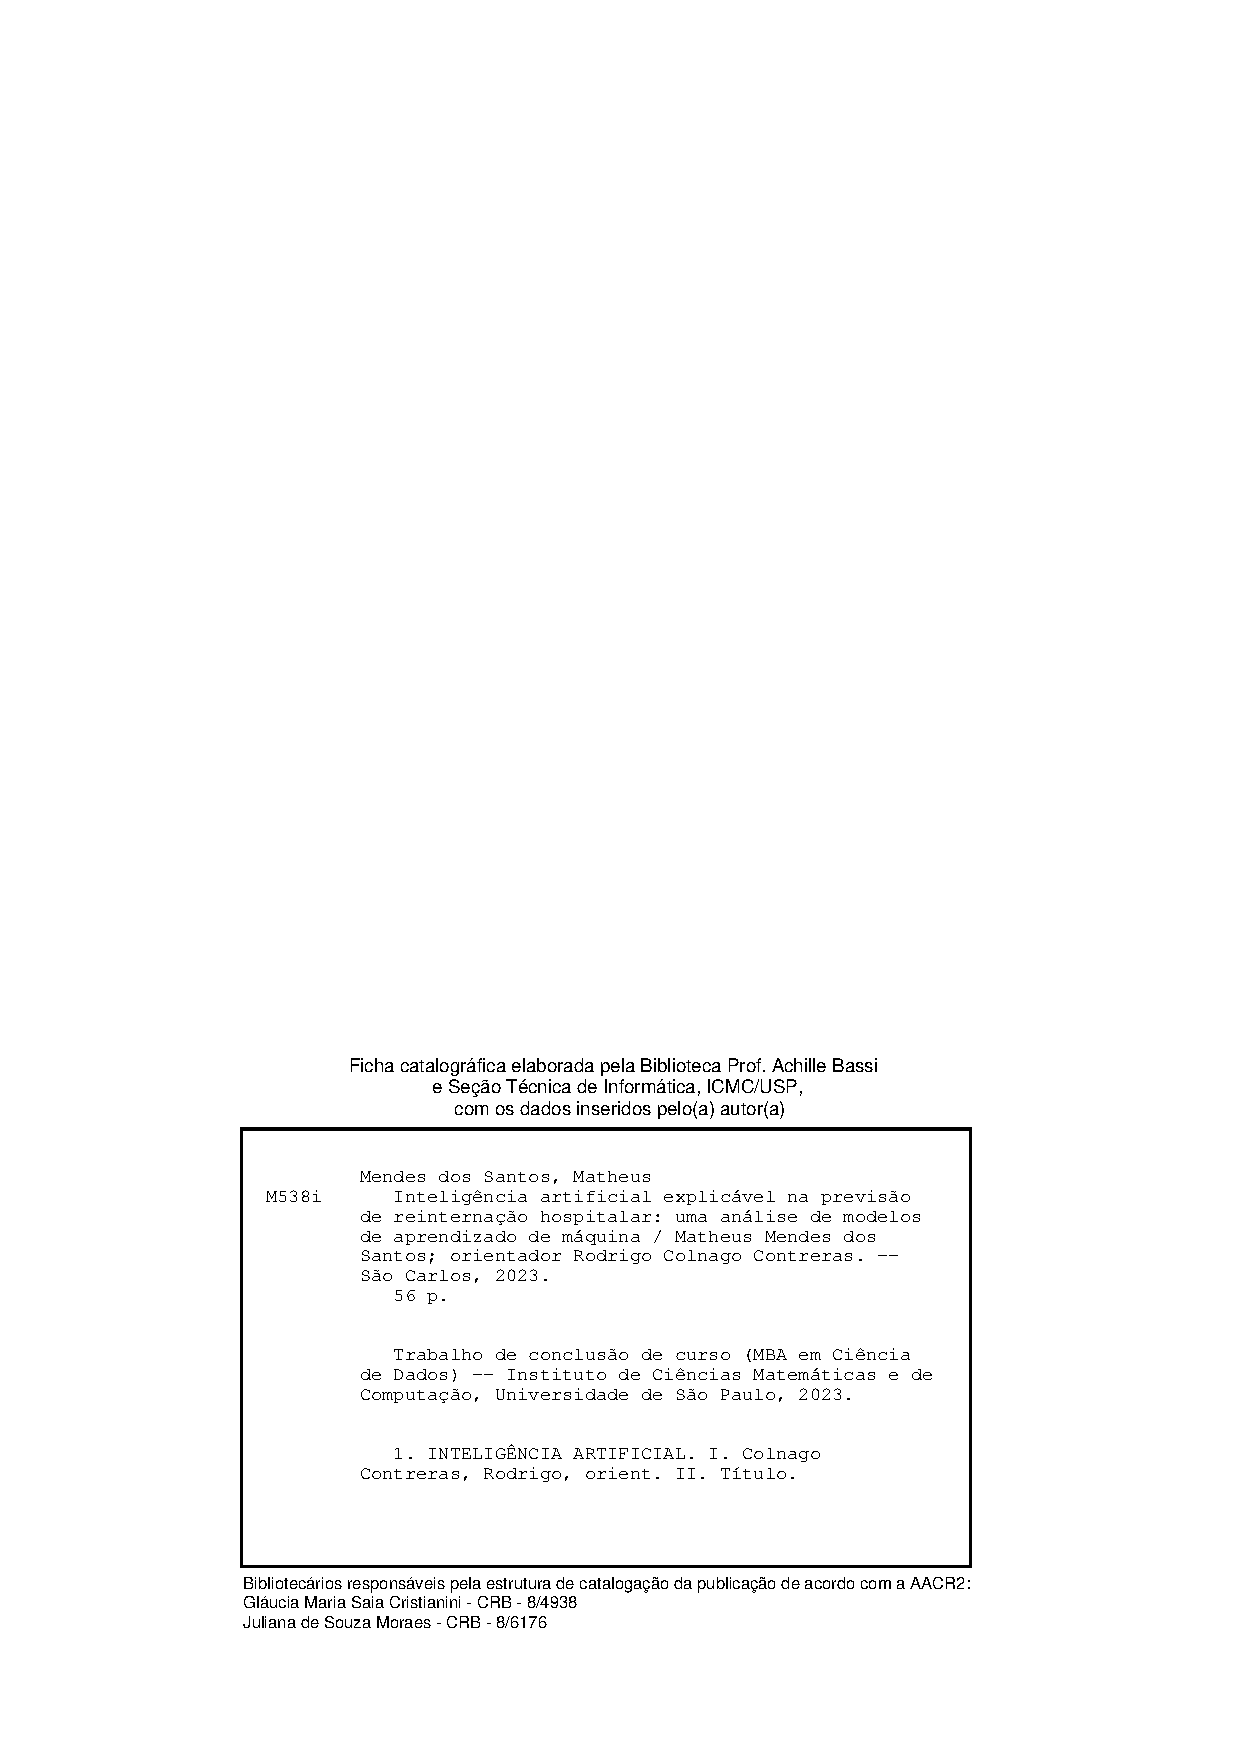
\includepdf{fichacatalografica.pdf}
			 %\end{fichacatalografica}
			 % Se você optar por elaborar a ficha catalográfica, deverá 
			 % incluir uma % antes das 3 linhas acima e tirar a % antes
			 % do comando %% USPSC-fichacatalografica.tex
% ---
% Inserir a ficha bibliografica
% ---
% Isto é um exemplo de Ficha Catalográfica, ou ``Dados internacionais de
% catalogação-na-publicação''. Você pode utilizar este modelo como referência. 
% Porém, provavelmente a biblioteca da sua universidade lhe fornecerá um PDF
% com a ficha catalográfica definitiva após a defesa do trabalho. Quando estiver
% com o documento, salve-o como PDF no diretório do seu projeto e substitua todo
% o conteúdo de implementação deste arquivo pelo comando abaixo:
%
\begin{fichacatalografica}
	\hspace{-1.4cm}
	\imprimirnotaautorizacao \\ \\
	%\sffamily
	\vspace*{\fill}					% Posição vertical
\begin{center}					% Minipage Centralizado
  \imprimirnotabib \\
  \begin{table}[htb]
	\scriptsize
	\centering	
	\begin{tabular}{|p{0.9cm} p{8.7cm}|}
		\hline
	      & \\
		  &	  \imprimirautorficha     \\
		
		 \imprimircutter & 
							\hspace{0.4cm}\imprimirtitulo~  / ~\imprimirautor~ ;  ~\imprimirorientadorcorpoficha. -- 	\imprimirlocal, \imprimirdata.   \\
		
		  &  % Para incluir nota referente à versão corrigida no corpo da ficha,
			  % incluir % no início da linha acima e tirar a % do início da linha abaixo
			  %	\hspace{0.4cm} \imprimirtitulo~  / ~\imprimirautor~ ; ~\imprimirorientadorcorpoficha~- ~\imprimirnotafolharosto. -- \imprimirlocal, \imprimirdata.  \\
		
			\hspace{0.4cm}\pageref{LastPage} p. : il. (algumas color.) ; 30 cm.\\ 
		  & \\
		  & 
		    \hspace{0.4cm}\imprimirnotaficha ~--~ 
						  \imprimirunidademin, 
						  \imprimiruniversidademin, 
		                  \imprimirdata. \\ 
		  & \\                 
		   % Para incluir nota referente à versão corrigida em notas,
		    % incluir uma % no início da linha acima e	
		    % tirar a % do início da linha abaixo
		    % & \hspace{0.4cm}\imprimirnotafolharosto \\ 
		  & \\ 
		  & \hspace{0.4cm}1. LaTeX. 2. abnTeX. 3. Classe USPSC. 4. Editoração de texto. 5. Normalização da documentação. 6. Tese. 7. Dissertação. 8. Documentos (elaboração). 9. Documentos eletrônicos. I. \imprimirorientadorficha. 
		   II. Título. \\
	
		     %Se houver co-orientador, inclua % antes da linha (antes de II. Título.) 
		     %          e tire a % antes do comando abaixo 
		     %III. Título. \\   
		  \hline
	\end{tabular}
  \end{table}
\end{center}
\end{fichacatalografica}
% ---


			 %% USPSC-fichacatalografica.tex
% ---
% Inserir a ficha bibliografica
% ---
% Isto é um exemplo de Ficha Catalográfica, ou ``Dados internacionais de
% catalogação-na-publicação''. Você pode utilizar este modelo como referência. 
% Porém, provavelmente a biblioteca da sua universidade lhe fornecerá um PDF
% com a ficha catalográfica definitiva após a defesa do trabalho. Quando estiver
% com o documento, salve-o como PDF no diretório do seu projeto e substitua todo
% o conteúdo de implementação deste arquivo pelo comando abaixo:
%
\begin{fichacatalografica}
	\hspace{-1.4cm}
	\imprimirnotaautorizacao \\ \\
	%\sffamily
	\vspace*{\fill}					% Posição vertical
\begin{center}					% Minipage Centralizado
  \imprimirnotabib \\
  \begin{table}[htb]
	\scriptsize
	\centering	
	\begin{tabular}{|p{0.9cm} p{8.7cm}|}
		\hline
	      & \\
		  &	  \imprimirautorficha     \\
		
		 \imprimircutter & 
							\hspace{0.4cm}\imprimirtitulo~  / ~\imprimirautor~ ;  ~\imprimirorientadorcorpoficha. -- 	\imprimirlocal, \imprimirdata.   \\
		
		  &  % Para incluir nota referente à versão corrigida no corpo da ficha,
			  % incluir % no início da linha acima e tirar a % do início da linha abaixo
			  %	\hspace{0.4cm} \imprimirtitulo~  / ~\imprimirautor~ ; ~\imprimirorientadorcorpoficha~- ~\imprimirnotafolharosto. -- \imprimirlocal, \imprimirdata.  \\
		
			\hspace{0.4cm}\pageref{LastPage} p. : il. (algumas color.) ; 30 cm.\\ 
		  & \\
		  & 
		    \hspace{0.4cm}\imprimirnotaficha ~--~ 
						  \imprimirunidademin, 
						  \imprimiruniversidademin, 
		                  \imprimirdata. \\ 
		  & \\                 
		   % Para incluir nota referente à versão corrigida em notas,
		    % incluir uma % no início da linha acima e	
		    % tirar a % do início da linha abaixo
		    % & \hspace{0.4cm}\imprimirnotafolharosto \\ 
		  & \\ 
		  & \hspace{0.4cm}1. LaTeX. 2. abnTeX. 3. Classe USPSC. 4. Editoração de texto. 5. Normalização da documentação. 6. Tese. 7. Dissertação. 8. Documentos (elaboração). 9. Documentos eletrônicos. I. \imprimirorientadorficha. 
		   II. Título. \\
	
		     %Se houver co-orientador, inclua % antes da linha (antes de II. Título.) 
		     %          e tire a % antes do comando abaixo 
		     %III. Título. \\   
		  \hline
	\end{tabular}
  \end{table}
\end{center}
\end{fichacatalografica}
% ---


			 % As informações que compõem a ficha catalográfica estão 
			 % definidas no arquivo USPSC-pre-textual-UUUU.tex
			 % ---
			 \end{verbatim} 
			 				
É possível incluir ou não o Código Cutter na ficha catalográfica, conforme a seguinte orientação nos respectivos arquivos pré-textuais:

\begin{verbatim}
\cutter{S856m}
% Para gerar a ficha catalográfica sem o Código Cutter, basta 
% incluir uma % na linha acima e tirar a % da linha abaixo
%\cutter{ } 
\end{verbatim} 

Através do arquivo fichacatalografica.tex é possível elaborar a ficha catalográfica em \LaTeX\ . Caso o trabalho possua co-orientador será necessário seguir as orientações contidas também no arquivo com os elementos pré-textuais.	 


\section{Resultados de comandos}\label{sec-divisoes}

O conteúdo desta seção foi baseado no item \textbf{1 Resultados de comandos} do \textbf{Modelo canônico de trabalho acadêmico com abnTEX2} \cite{equipeabntex2}.

% ---
\subsection{Codificação dos arquivos: UTF8}
% ---

A codificação \texttt{UTF8} deve ser utilizada para todos os arquivos do \abnTeX\ . Utilize a mesma codificação nos documentos que escrever, incluindo nos arquivos de bases bibliográficas |.bib|. Para tanto, tanto o arquivo USPSC-modelo.tex  quanto o USPSC-TCC-modelo.tex devem conter o seguinte pacote:

\begin{verbatim}
\usepackage[utf8]{inputenc}	 % Codificacao do documento (conversão
                               automática dos acentos)
\end{verbatim}

% ---
\subsection{Diferentes idiomas e hifenizações}
\label{sec-hifenizacao}
% ---

Para usar hifenizações de diferentes idiomas, inclua nas opções do documento o
nome dos idiomas que o seu texto contém. Os usuários da Classe USPSC devem utilizar:

\begin{verbatim}
\documentclass[
% -- opções da classe memoir --
12pt,		% tamanho da fonte
openright,	% capítulos começam em pág ímpar (insere página vazia caso 
preciso)
twoside,  % para impressão em anverso (frente) e verso. Oposto a oneside - 
Nota: utilizar \imprimirfolhaderosto*
%oneside, % para impressão em páginas separadas (somente anverso) -  
Nota: utilizar \imprimirfolhaderosto
% inclua uma % antes do comando twoside e exclua a % antes do oneside 
a4paper,			% tamanho do papel. 
% -- opções da classe abntex2 --
chapter=TITLE,		% títulos de capítulos convertidos em letras 
maiúsculas
% -- opções do pacote babel --
english,			% idioma adicional para hifenização
french,				% idioma adicional para hifenização
spanish,			% idioma adicional para hifenização
brazil				% o último idioma é o principal do documento
% {USPSC-classe/USPSC} configura o cabeçalho contendo apenas o número 
da página
]{USPSC-classe/USPSC}
%]{USPSC-classe/USPSC1}
% Inclua % antes de ]{USPSC-classe/USPSC} e retire a % antes 
de %]{USPSC-classe/USPSC1} para utilizar o 
% cabeçalho diferenciado para as páginas pares e ímpares:
%- páginas ímpares: cabeçalho com seções ou subseções e o número da página
%- páginas pares: cabeçalho com o número da página e o título do capítulo 
% ---
\end{verbatim}

Desta forma o texto deverá ser escrito idioma português-brasileiro (\texttt{brazil}), podendo ter citações em inglês, francês e espanhol.

O idioma português-brasileiro (\texttt{brazil}) é incluído automaticamente pela
classe \textsf{abntex2}. Porém, mesmo assim a opção \texttt{brazil} deve ser
informada como a última opção da classe para que todos os pacotes reconheçam o
idioma. Vale ressaltar que a última opção de idioma é a utilizada por padrão no
documento. 

Portanto, para Classe USPSC, caso deseje escrever um texto em inglês que tenha
citações em espanhol, português e francês, você deverá usar:

\begin{verbatim}
\documentclass[
% -- opções da classe memoir --
12pt,		% tamanho da fonte
openright,	% capítulos começam em pág ímpar (insere página vazia caso 
preciso)
twoside,  % para impressão em anverso (frente) e verso. Oposto a oneside - 
Nota: utilizar \imprimirfolhaderosto*
%oneside, % para impressão em páginas separadas (somente anverso) -  
Nota: utilizar \imprimirfolhaderosto
% inclua uma % antes do comando twoside e exclua a % antes do oneside 
a4paper,			% tamanho do papel. 
% -- opções da classe abntex2 --
chapter=TITLE,		% títulos de capítulos convertidos em letras 
maiúsculas
% -- opções do pacote babel --
spanish,			% idioma adicional para hifenização
french,				% idioma adicional para hifenização
brazil,				% o último idioma é o principal do documento
english 			% idioma adicional para hifenização
% {USPSC-classe/USPSC} configura o cabeçalho contendo apenas o número 
da página
]{USPSC-classe/USPSC}
%]{USPSC-classe/USPSC1}
% Inclua % antes de ]{USPSC-classe/USPSC} e retire a % antes 
de %]{USPSC-classe/USPSC1} para utilizar o 
% cabeçalho diferenciado para as páginas pares e ímpares:
%- páginas ímpares: cabeçalho com seções ou subseções e o número da página
%- páginas pares: cabeçalho com o número da página e o título do capítulo 
% ---
\end{verbatim}

A lista completa de idiomas suportados, bem como outras opções de hifenização,
estão disponíveis em \citeonline[p.~7-8]{babel2011}. \\

Exemplo de hifenização em inglês\footnote{Extraído de:
	\url{http://en.wikibooks.org/wiki/LaTeX/Internationalization}}:

\begin{otherlanguage*}{english}
	\textit{Text in English language. This environment switches all language-related
		definitions, like the language specific names for figures, tables etc. to the other
		language. The starred version of this environment typesets the main text
		according to the rules of the other language, but keeps the language specific
		string for ancillary things like figures, in the main language of the document.
		The environment hyphenrules switches only the hyphenation patterns used; it can
		also be used to disallow hyphenation by using the language name
		`nohyphenation'.}
\end{otherlanguage*}

Exemplo de hifenização em francês\footnote{Extraído de:
	\url{http://bigbrowser.blog.lemonde.fr/2013/02/17/tu-ne-tweeteras-point-le-vatican-interdit-aux-cardinaux-de-tweeter-pendant-le-conclave/}}:

\begin{otherlanguage*}{french}
	\textit{Texte en français. Pas question que Twitter ne vienne faire une
		concurrence déloyale à la traditionnelle fumée blanche qui marque l'élection
		d'un nouveau pape. Pour éviter toute fuite précoce, le Vatican a donc pris un
		peu d'avance, et a déjà interdit aux cardinaux qui prendront part au vote
		d'utiliser le réseau social, selon Catholic News Service. Une mesure valable
		surtout pour les neuf cardinaux – sur les 117 du conclave – pratiquants très
		actifs de Twitter, qui auront interdiction pendant toute la période de se
		connecter à leur compte.}
\end{otherlanguage*}

Exemplo de hifenização em espanhol\footnote{Extraído de:
	\url{http://internacional.elpais.com/internacional/2013/02/17/actualidad/1361102009_913423.html}}:

\foreignlanguage{spanish}{\textit{Decenas de miles de personas ovacionan al pontífice en su
		penúltimo ángelus dominical, el primero desde que anunciase su renuncia. El Papa se
		centra en la crítica al materialismo}}.

O idioma geral do texto pode ser alterado como no exemplo seguinte:

\begin{verbatim}
\selectlanguage{english}

\end{verbatim}

Isso altera automaticamente a hifenização e todos os nomes constantes de
referências do documento para o idioma inglês. Consulte o manual da classe para obter orientações adicionais sobre internacionalização de documentos produzidos com \textsf{\abnTeX} \cite{abnetxclasse}.

Se a opção de idioma do texto não for o português, é necessário observar o descrito em \ref{idioma}.

% ---
\subsection{Enumerações}
% ---

\index{alíneas}\index{subalíneas}\index{incisos}Quando for necessário enumerar
os diversos assuntos de uma seção que não possua título, esta deve ser
subdividida em alíneas \cite[4.2]{nbr6024}:

\begin{alineas}

  \item os diversos assuntos que não possuam título próprio, dentro de uma mesma
  seção, devem ser subdivididos em alíneas; 
  
  \item o texto que antecede as alíneas termina em dois pontos;
  \item as alíneas devem ser indicadas alfabeticamente, em letra minúscula
  seguida de parêntese. Utilizam-se letras dobradas, quando esgotadas as
  letras do alfabeto;

  \item as letras indicativas das alíneas devem apresentar recuo em relação à
  margem esquerda;

  \item o texto da alínea deve começar por letra minúscula e terminar em
  ponto-e-vírgula, exceto a última alínea que termina em ponto final;

  \item o texto da alínea deve terminar em dois pontos, se houver subalínea;

  \item a segunda e as seguintes linhas do texto da alínea começa sob a
  primeira letra do texto da própria alínea;
  
  \item subalíneas \cite{nbr6024} devem ser conforme as alíneas a
  seguir:

  \begin{alineas}
     \item as subalíneas devem começar por travessão seguido de espaço;

     \item as subalíneas devem apresentar recuo em relação à alínea;

     \item o texto da subalínea deve começar por letra minúscula e terminar em
     ponto-e-vírgula. A última subalínea deve terminar em ponto final, se não
     houver alínea subsequente;

     \item a segunda e as seguintes linhas do texto da subalínea começam sob a
     primeira letra do texto da própria subalínea.
  \end{alineas}
  
  \item no \abnTeX\ estão disponíveis os ambientes \texttt{incisos} e
  \texttt{subalineas}, que em suma é o mesmo que se criar outro nível de
  \texttt{alineas}, como nos exemplos à seguir:
  
  \begin{incisos}
    \item \textit{Um novo inciso em itálico};
  \end{incisos}
  
  \item Alínea em \textbf{negrito}:
  
  \begin{subalineas}
    \item \textit{Uma subalínea em itálico};
    \item \underline{\textit{Uma subalínea em itálico e sublinhado}}; 
  \end{subalineas}
  
  \item Última alínea com \emph{ênfase}.
  
\end{alineas}

% ---
\subsection{Espaçamento entre parágrafos e linhas}\label{sec_espacamento}
% ---

\index{espaçamento!dos parágrafos}O tamanho do parágrafo, espaço entre a margem
e o início da frase do parágrafo, é definido por:

\begin{verbatim}
   \setlength{\parindent}{1.3cm}
\end{verbatim}

\index{espaçamento!do primeiro parágrafo}Por padrão, não há espaçamento no
primeiro parágrafo de cada início de divisão do documento
(\autoref{sec-divisoes-b}). Porém, você pode definir que o primeiro parágrafo
também seja indentado, como é o caso deste documento. Para isso, apenas inclua o
pacote \textsf{indentfirst} no preâmbulo do documento:

\begin{verbatim}
   \usepackage{indentfirst} % Indenta o primeiro parágrafo de cada seção.
\end{verbatim}

\index{espaçamento!entre os parágrafos}O espaçamento entre um parágrafo e outro
pode ser controlado por meio do comando:

\begin{verbatim}
  \setlength{\parskip}{0.2cm}  % tente também \onelineskip
\end{verbatim}

\index{espaçamento!entre as linhas}O controle do espaçamento entre linhas é
definido por:
\begin{verbatim}
  \OnehalfSpacing       % espaçamento um e meio (padrão); 
  \DoubleSpacing        % espaçamento duplo
  \SingleSpacing        % espaçamento simples	
\end{verbatim}

Para isso, também estão disponíveis os ambientes:
\begin{verbatim}
  \begin{SingleSpace} ...\end{SingleSpace}
  \begin{Spacing}{hfactori} ... \end{Spacing}
  \begin{OnehalfSpace} ... \end{OnehalfSpace}
  \begin{OnehalfSpace*} ... \end{OnehalfSpace*}
  \begin{DoubleSpace} ... \end{DoubleSpace}
  \begin{DoubleSpace*} ... \end{DoubleSpace*} 
\end{verbatim}

% ---
\subsection{Tabelas e quadros}

As tabelas e os quadros apresentam os dados de modo resumido, oferecendo uma visão geral do conteúdo em questão, visando facilitar a compreensão do fenômeno em estudo. A diferença básica entre ambas está relacionada ao conteúdo e a formatação. 

Tabela é o conjunto de dados estatísticos, dispostos em determinada ordem de classificação, que expressam as variações qualitativas de um fenômeno. Sua finalidade básica é resumir ou sintetizar dados \cite{sibi2016}.

A construção de tabelas deve obedecer os critérios estabelecidos pelo Instituto Brasileiro de Geografia e Estatística (IBGE) e requeridos pelas normas da ABNT para documentos técnicos e acadêmicos.

A \autoref{tab-ibge} é um exemplo de tabela alinhada que pode ser longa ou curta, conforme padrão do IBGE.

\begin{table}[htb]
	%\begin{table}[H]
	\IBGEtab{%
		\caption{Frequência anual por categoria de usuários}%
		\label{tab-ibge}
	}{%
	\begin{tabular}{ccc}
		\toprule
		Categoria de Usuários & Frequência de Usuários \\
		\midrule \midrule
		Graduação & 72\% \\
		\midrule 
		Pós-Graduação & 15\% \\
		\midrule 
		Docente & 10\% \\
		\midrule 
		Outras & 3\% \\
		\bottomrule
	\end{tabular}%
}{%
\fonte{Elaborada pelos autores.}%
\nota{Exemplo de uma nota.}%
\nota[Anotações]{Uma anotação adicional, que pode ser seguida de várias
	outras.}%

}
\end{table}


\begin{table}[H]
	\IBGEtab{%
		\caption{Níveis descritivos dos testes de comparação de médias entre grupos para profundidade da lesão junto à restauração}%
		\label{tabela-ibge}
	}{%
	\begin{tabular}{p{5.5cm}|p{5.5cm}}
		\hline
		\textbf{Resultado} & \textbf{Nível Descritivo} \\ 
		\hline 
		CIC < Ariston & < 0,0001  \\
		Ariston < Am & 0,0118  \\
		Am = Helio & 0,4576  \\
		-100 = Helio & 0,3360  \\
		\hline
	\end{tabular}%
}{%
\fonte{\citeonline{sibi2009}}%
}
\end{table} 

Os \textbf{APÊNDICES J-K} exemplificam outras formatações de tabelas.

A formatação do quadro é similar à tabela, mas deve ter suas laterais fechadas e conter as linhas horizontais.

% o comando \newpage foi utilizado para forçar a quebra de página

\begin{quadro}[htb]
	\caption{\label{quadro_modelo}Níveis de investigação}
	\begin{tabular}{|p{2.6cm}|p{6.0cm}|p{2.25cm}|p{3.40cm}|}
		\hline
		\textbf{Nível de Investigação} & \textbf{Insumos}  & \textbf{Sistemas de Investigação}  & \textbf{Produtos}  \\
		\hline
		Meta-nível & Filosofia\index{filosofia} da Ciência  & Epistemologia &
		Paradigma  \\
		\hline
		Nível do objeto & Paradigmas do metanível e evidências do nível inferior &
		Ciência  & Teorias e modelos \\
		\hline
		Nível inferior & Modelos e métodos do nível do objeto e problemas do nível inferior & Prática & Solução de problemas  \\
		\hline
	\end{tabular}
	\begin{flushleft}
		%\fonte{\citeonline{van1986}}
		Fonte: \citeonline{van1986}
	\end{flushleft}
\end{quadro} 


Os \textbf{APÊNDICES B-I} apresentam exemplos de quadros.

% ---
\subsection{Figuras}\label{sec_figuras}
% ---
\index{figuras}Figuras podem ser criadas diretamente em \LaTeX,
como o exemplo da \autoref{fig_circulo}. \\ 

\begin{figure}[htb]
	\caption{\label{fig_circulo}A delimitação do espaço}
	\begin{center}
		\setlength{\unitlength}{9cm}
		\begin{picture}(1,1)
		\put(0,0){\line(0,1){1}}
		\put(0,0){\line(1,0){1}}
		\put(0,0){\line(1,1){1}}
		\put(0,0){\line(1,2){.5}}
		\put(0,0){\line(1,3){.3333}}
		\put(0,0){\line(1,4){.25}}
		\put(0,0){\line(1,5){.2}}
		\put(0,0){\line(1,6){.1667}}
		\put(0,0){\line(2,1){1}}
		\put(0,0){\line(2,3){.6667}}
		\put(0,0){\line(2,5){.4}}
		\put(0,0){\line(3,1){1}}
		\put(0,0){\line(3,2){1}}
		\put(0,0){\line(3,4){.75}}
		\put(0,0){\line(3,5){.6}}
		\put(0,0){\line(4,1){1}}
		\put(0,0){\line(4,3){1}}
		\put(0,0){\line(4,5){.8}}
		\put(0,0){\line(5,1){1}}
		\put(0,0){\line(5,2){1}}
		\put(0,0){\line(5,3){1}}
		\put(0,0){\line(5,4){1}}
		\put(0,0){\line(5,6){.8333}}
		\put(0,0){\line(6,1){1}}
		\put(0,0){\line(6,5){1}}
		\end{picture}
	\end{center}
	\legend{Fonte: \citeonline{equipeabntex2}}
\end{figure}

Outra opção é incorporar a figura utilizando um arquivo externo, como é o caso da \autoref{fig_grafico}. Se a figura que for incluída se tratar de um diagrama, um gráfico ou uma ilustração, que você mesmo produza, priorize o uso de imagens vetoriais no formato PDF. Com isso, o tamanho do arquivo final do trabalho será menor e as imagens terão uma apresentação melhor, principalmente quando impressas, uma vez que imagens vetoriais são perfeitamente escaláveis para qualquer dimensão. Nesse caso, se for utilizar o Microsoft Excel para produzir gráficos, ou o Microsoft Word para ilustrações, exporte-os como PDF e os incorpore ao documento conforme o exemplo abaixo. No entanto, para manter a
coerência no uso de software livre (já que você está usando \LaTeX\  e \abnTeX),
teste a ferramenta \textsf{InkScape}\index{InkScape}
(\url{http://inkscape.org/}). Ela é uma excelente opção de código-livre para
produzir ilustrações vetoriais, similar ao CorelDraw\index{CorelDraw} ou ao Adobe
Illustrator\index{Adobe Illustrator}. De todo modo, caso não seja possível
utilizar arquivos de imagens como PDF, utilize qualquer outro formato, como
JPEG, GIF, BMP, etc. Nesse caso, você pode tentar aprimorar as imagens
incorporadas com o software livre \textsf{Gimp}\index{Gimp}
(\url{http://www.gimp.org/}). Ele é uma alternativa livre ao Adobe
Photoshop\index{Adobe Photoshop}. \\

\begin{figure}[H]
	\caption{\label{fig_grafico}Gráfico produzido em Excel e salvo como PDF}
	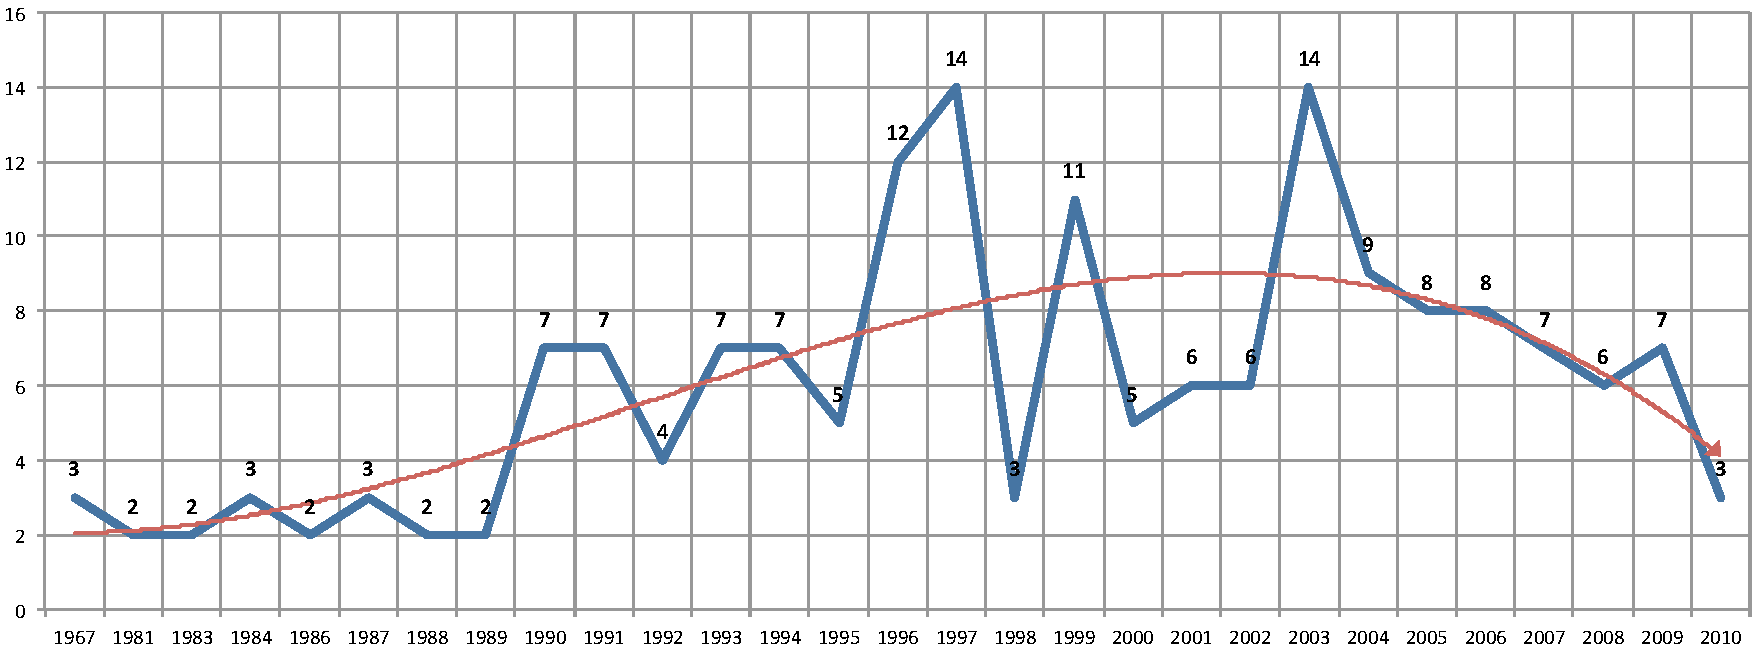
\includegraphics[scale=0.5]{USPSC-img/USPSC-modelo-img-grafico.pdf}
	\begin{flushleft}
		Fonte: \citeonline[p. 24]{araujo2012}
	\end{flushleft}	
\end{figure}

% ---
\subsubsection{Figuras em minipages}
% ---

As ilustrações devem sempre ter numeração contínua e única em todo o documento:

% O comando \newpage força a quebra de página

\begin{citacao}
	Qualquer que seja o tipo de ilustração, sua identificação aparece na parte
	superior, precedida da palavra designativa (desenho, esquema, fluxograma,
	fotografia, gráfico, mapa, organograma, planta, quadro, retrato, figura,
	imagem, entre outros), seguida de seu número de ordem de ocorrência no texto,
	em algarismos arábicos, travessão e do respectivo título. Após a ilustração, na
	parte inferior, indicar a fonte consultada (elemento obrigatório, mesmo que
	seja produção do próprio autor), legenda, notas e outras informações
	necessárias à sua compreensão (se houver). A ilustração deve ser citada no
	texto e inserida o mais próximo possível do trecho a que se
	refere \cite{nbr14724}.
\end{citacao}

\emph{Minipages} são usadas para inserir textos ou outros elementos em quadros
com tamanhos e posições controladas. Veja o exemplo da
\autoref{fig_minipage_imagem1} e da \autoref{fig_minipage_grafico2}.

\begin{figure}[H]
	\label{teste}
	\centering
	\begin{minipage}{0.4\textwidth}
		\centering
		\caption{Imagem 1 da minipage} \label{fig_minipage_imagem1}
		
\includegraphics[scale=0.9]{USPSC-img/USPSC-modelo-img-marca.pdf}
		\legend{Fonte: \citeonline{equipeabntex2}}
	\end{minipage}
	\hfill
	\begin{minipage}{0.4\textwidth}
		\centering
		\caption{Grafico 2 da minipage} \label{fig_minipage_grafico2}
		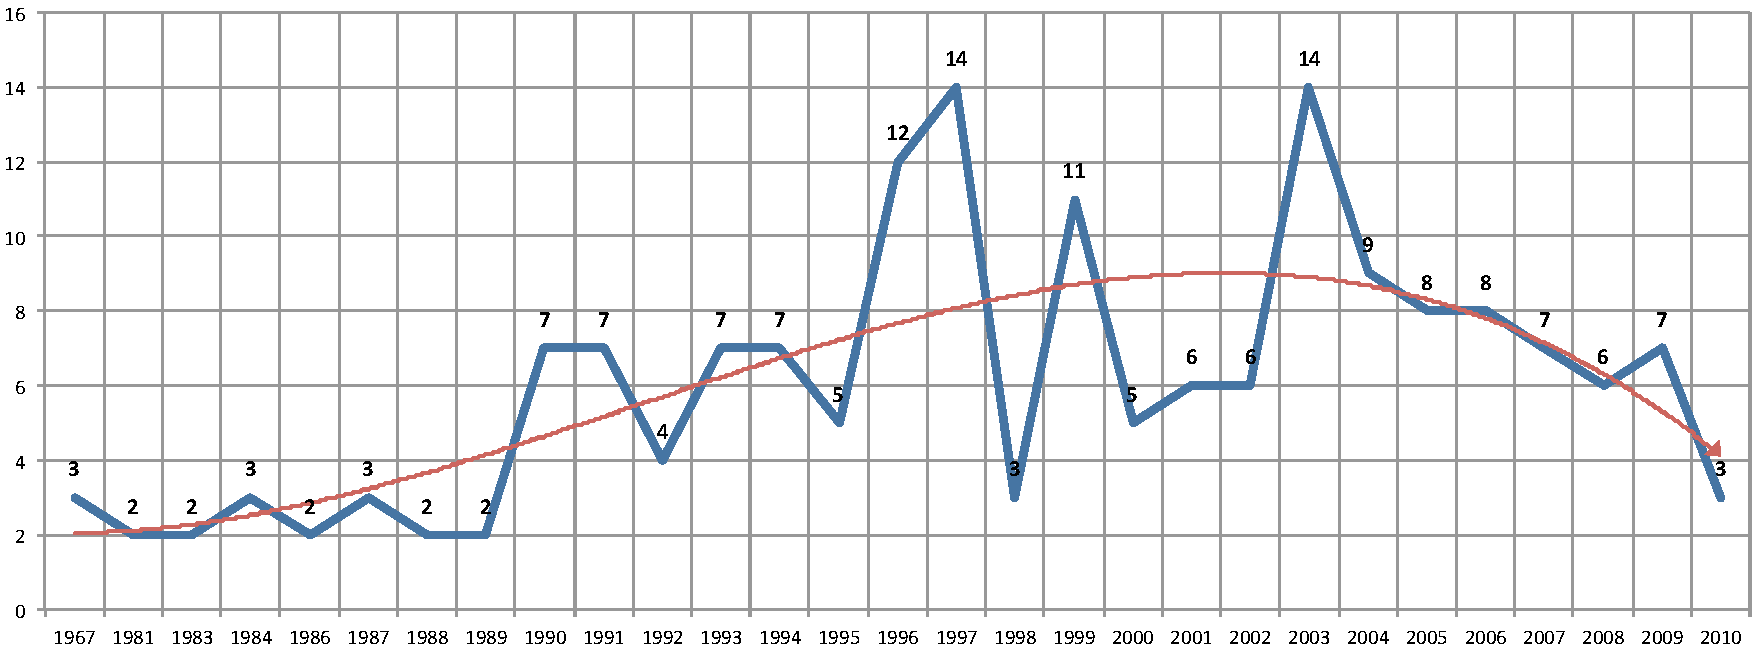
\includegraphics[scale=0.2]{USPSC-img/USPSC-modelo-img-grafico.pdf}
		\legend{Fonte: \citeonline[p. 24]{araujo2012}}
	\end{minipage}
\end{figure}

% ---
\subsection{Expressões matemáticas}
% ---

\index{expressões matemáticas}Use o ambiente \texttt{equation} para escrever
expressões matemáticas numeradas:

\begin{equation}
\forall x \in X, \quad \exists \: y \leq \epsilon
\end{equation}

Escreva expressões matemáticas entre \$ e \$, como em $ \lim_{x \to \infty}
\exp(-x) = 0 $, para que fiquem na mesma linha.

Também é possível usar colchetes para indicar o início de uma expressão
matemática que não é numerada.

\[
\left|\sum_{i=1}^n a_ib_i\right|
\le
\left(\sum_{i=1}^n a_i^2\right)^{1/2}
\left(\sum_{i=1}^n b_i^2\right)^{1/2}
\]

Consulte mais informações sobre expressões matemáticas em
\url{https://github.com/abntex/abntex2/wiki/Referencias}.

\subsection{Estruturas, reações e mecanismos de reações químicas}\label{Reaquimica}
Para a versão 3.0 do Pacote USPSC, o Grupo Desenvolvedor optou por utilizar os pacotes \textbf{mychemistry},  \textbf{ChemFig} e o \textbf{TikZ}, que fornecem comandos que permitem compor esquemas complexos de reação química com \LaTeX\ . 

Aqui são apresentados alguns exemplos, sendo que a maioria foram retirados do manual do pacote \textbf{ChemFig}\cite{ChemFigPac}. 


A fórmula estrutural do metano é:


\chemfig{C(-[5]H)(-[2]H)(<[:-70]H)(<:[:-20]H)} \\

\begin{verbatim}
\end{verbatim} 

Molecula da Adrenalina é:

\chemfig{*6((-HO)-=-(-(<[::60]OH)-[::-60]-[::-60,,,2]
	HN-[::+60]CH_3)=-(-HO)=)} \\

\begin{verbatim}
\end{verbatim}

Com o comando abaixo, o \textbf{ChemFig} possibilita escrever o nome de uma molécula abaixo dela. 

\begin{verbatim}
\ chemname [hdimi] {\ chemfig {código da molécula}} {hnamei}
\end{verbatim}

Para exemplificar apresentamos uma reação com os nomes das respectivas moléculas:

\schemestart
\chemname{\chemfig{R-C(-[:-30]OH)=[:30]O}}{Ácido carboxílico}
\+
\chemname{\chemfig{R’OH}}{Álcool}
\arrow(.mid east--.mid west)
\chemname{\chemfig{R-C(-[:-30]OR’)=[:30]O}}{Éster}
\+
\chemname{\chemfig{H_2O}}{Água}
\schemestop
\chemnameinit{}
 \\

\begin{verbatim}
\end{verbatim}

Mediante a utilização dos pacotes \textbf{TikZ} e \textbf{ChemFig}, o pacote \textbf{xcolor} é carregado possibilitando o uso de cores nos códigos de comandos, conforme exemplos abaixo:

\chemfig{C|{\color{blue}H_3}-C(=[1]O)-[7]O|{\color{red}H}} 

\begin{verbatim}
\end{verbatim}

Para destacar substâncias individualmente ou parte de um esquema, é possível utilizar recursos tais como os exemplificados a seguir.

\begin{verbatim}
setchemfig{compound style={draw,line width=0.8pt,
semitransparent,text opacity=1,inner sep=8pt,
rounded corners=1mm}}
\schemestart
A\arrow([fill=red]--[fill=blue])[90]
B\arrow(--[fill=gray])
C\arrow(--[fill=green])[-90]
D\arrow(--[draw=none])[-180]
\schemestop
\end{verbatim} 

\begin{verbatim}
\end{verbatim}



\setchemfig{compound style={draw,line width=0.8pt,
		semitransparent,text opacity=1,inner sep=8pt,
		rounded corners=1mm}}
\schemestart
A\arrow([fill=red]--[fill=blue])[90]
B\arrow(--[fill=gray])
C\arrow(--[fill=green])[-90]
D\arrow(--[draw=none])[-180]
\schemestop

\begin{verbatim}
\end{verbatim} 

Mais um exemplo de utilização dos recursos do pacote TikZ é o desenho de duas linhas e um ponto de interseção. O comando \verb+ \draw[blue, thick] + define um elemento gráfico cuja cor é azul e com um traço grosso. A linha é definida por seus dois pontos finais, (-1,2) e (2, -4), unidos por -. O comando \verb+ \filldraw[red] (0,0) circle (2pt) + \\ \verb+node[anchor=west] {Intersection point} + irá desenhar um círculo preenchido com a cor vermelha, sendo que (0,0) define o ponto central, (2pt) determina o raio e, próximo ao ponto, um nó e uma caixa contendo o texto "ponto de interseção", ancorado a oeste do ponto.


\begin{verbatim}
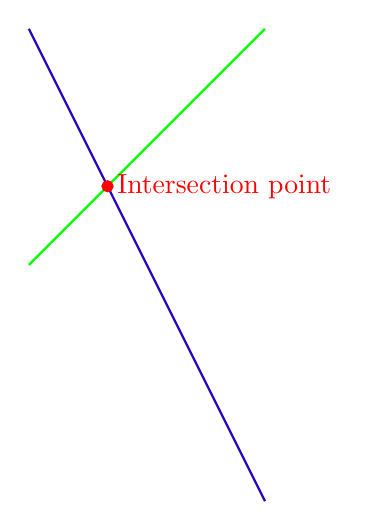
\begin{tikzpicture}
\draw[blue, thick] (-1,2) -- (2,-4);
\draw[green, thick] (-1,-1) -- (2,2);
\filldraw[red] (0,0) circle (2pt) node[anchor=west] {Intersection point};
\end{tikzpicture}
\end{verbatim}

Tais comandos geram os elementos gráficos abaixo:

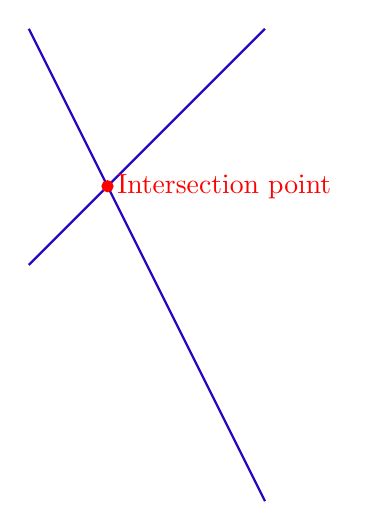
\begin{tikzpicture}
\draw[blue, thick] (-1,2) -- (2,-4);
\draw[blue, thick] (-1,-1) -- (2,2);
\filldraw[red] (0,0) circle (2pt) node[anchor=west] {Intersection point};
\end{tikzpicture}


Para gerar este documento, no preâmbulo do arquivo principal (USPSC-modelo.tex e USPSC-TCC-modelo.tex ) foram incluídos os seguintes comandos:
\begin{verbatim}
\usepackage{float} 				% Fixa tabelas e figuras no local exato
\usepackage{chemfig,chemmacros} % Para escrever reações químicas
\usepackage{mychemistry}        % Para escrever reações químicas
\usepackage{tikz}               % Para escrever reações químicas e outros
\usetikzlibrary{arrows, babel}	% Para escrever reações químicas e outros
\end{verbatim}

Para informações complementares e recursos adicionais, consulte os manuais dos pacotes utilizados:  \textbf{mychemistry}\cite{mychemistryPac}, \textbf{ChemFig}\cite{ChemFigPac}, \textbf{etoolbox}\cite{etoolboxPack}, \textbf{float}\cite{floatPac}, \textbf{xkeyval}\cite{xkeyvalPac}, \textbf{chemmacros}\cite{chemmacrosPac}, \textbf{TikZ e PGF}\cite{TikZPac} ou de outros necessários para o seu documento.


% ---
\subsection{Inclusão de outros arquivos}\label{sec-include}
% ---

É uma boa prática dividir o seu documento em diversos arquivos, e não
apenas escrever tudo em um único. Esse recurso foi utilizado neste
documento. Para incluir diferentes arquivos em um arquivo principal,
de modo que cada arquivo incluído fique em uma página diferente, utilize o
comando:

\begin{verbatim}
   \include{documento-a-ser-incluido}      % sem a extensão .tex
\end{verbatim}

Para incluir documentos sem quebra de páginas, utilize:

\begin{verbatim}
   \input{documento-a-ser-incluido}      % sem a extensão .tex
\end{verbatim}
% ---
\subsection{Índice(s)}
% ---
Elemento  opcional,  que  consiste  em  lista  de  palavras  ou  frases  ordenadas alfabeticamente (autor, título ou assunto) ou sistematicamente (ordenação por classes, numérica ou cronológica); localiza e remete para as informações contidas no texto. A paginação deve ser contínua, dando seguimento ao texto principal \cite{aguia2020}.

Para criar índice remissivo no \LaTeX\  utilize o pacote makeidx, que deve estar declarado com os demais pacotes. No presente modelo está declarado no arquivo USPSC-modelo.tex, conforme indicado abaixo:

\begin{verbatim}
% ---
% Pacotes básicos - Fundamentais 
% ---
\usepackage[T1]{fontenc}		% Seleção de códigos de fonte.
\usepackage[utf8]{inputenc}		% Codificação do documento (conversão 
automática dos acentos)
\usepackage{lmodern}			% Usa a fonte Latin Modern
% Para utilizar a fonte Times New Roman, inclua uma % no início do comando 
acima  "\usepackage{lmodern}"
% Abaixo, tire a % antes do comando  \usepackage{times}
%\usepackage{times}		    	% Usa a fonte Times New Roman	
% Lembre-se de alterar a fonte no comando que imprime o preâmbulo no 
arquivo da Classe USPSC.cls				
\usepackage{lastpage}			% Usado pela Ficha catalográfica
\usepackage{indentfirst}		% Indenta o primeiro parágrafo de cada seção.
\usepackage{color}				% Controle das cores
\usepackage{graphicx}			% Inclusão de gráficos
\usepackage{float} 				% Fixa tabelas e figuras no local exato
\usepackage{chemfig,chemmacros} % Para escrever reações químicas
\usepackage{mychemistry}        % Para escrever reações químicas
\usepackage{tikz}				% Para escrever reações químicas e outros
\usetikzlibrary{arrows, babel}	% Para escrever reações químicas e outros
\usepackage{microtype} 			% para melhorias de justificação
\usepackage{pdfpages}
\usepackage{makeidx}            % para gerar índice remissivo
% ---
\end{verbatim}

A habilitação dos comandos de indexação foi incluída no arquivo USPSC-modelo.tex da seguinte forma:


\begin{verbatim}
% compila o sumário e índice
\makeindex
% ---
\end{verbatim}

O presente modelo inclui um exemplo de índice, gerado a partir da utilização de comandos similares aos reproduzidos abaixo:

\begin{verbatim}
\index{InkScape}
\index{CorelDraw}
\index{Adobe Illustrator}
\index{Gimp}
\index{Adobe Photoshop}
\index{espaçamento!do primeiro parágrafo}
\index{espaçamento!dos parágrafos}
\index{espaçamento!entre as linhas}
\index{espaçamento!entre os parágrafos}
\end{verbatim}

Os comandos acima estão no arquivo USPSC-Cap2-Desenvolvimento.tex, em textos na  \autoref{sec_espacamento}  e na  \autoref{sec_figuras}.

Para imprimir o índice, no final do arquivo USPSC-modelo.tex foi incluído:

\begin{verbatim}

%---------------------------------------------------------------------
% INDICE REMISSIVO
%--------------------------------------------------------------------
\phantompart
\printindex
%---------------------------------------------------------------------
\end{verbatim}

Para que o índice seja gerado e incluído corretamente no texto é necessário compilá-lo separadamente. No \textbf{TeXstudio 2.9.4}, na barra de menu, selecione \textbf{Tools} e execute \textbf{Index}.


% ---
\subsection{Compilar o documento \LaTeX}
% ---

Geralmente os editores \LaTeX, como o
TeXlipse\footnote{\url{http://texlipse.sourceforge.net/}}, o
Texmaker\footnote{\url{http://www.xm1math.net/texmaker/}}, entre outros,
compilam os documentos automaticamente, de modo que você não precisa se
preocupar com isso.

No entanto, você pode compilar os documentos \LaTeX\ usando os seguintes
comandos, que devem ser digitados no \emph{Prompt de Comandos} do Windows ou no
\emph{Terminal} do Mac ou do Linux:

\begin{verbatim}
   pdflatex ARQUIVO_PRINCIPAL.tex
   bibtex ARQUIVO_PRINCIPAL.aux
   makeindex ARQUIVO_PRINCIPAL.idx 
   makeindex ARQUIVO_PRINCIPAL.nlo -s nomencl.ist -o ARQUIVO_PRINCIPAL.nls
   pdflatex ARQUIVO_PRINCIPAL.tex
   pdflatex ARQUIVO_PRINCIPAL.tex
\end{verbatim}

% ---
\subsection{Remissões internas}
% ---

Ao nomear a \autoref{tab-ibge} e a \autoref{fig_circulo}, apresentamos um exemplo de remissão interna, que também pode ser feita quando indicamos o
\autoref{cap_exemplos}, que tem o nome \emph{\nameref{cap_exemplos}}. O número
do capítulo indicado é \ref{cap_exemplos}, que se inicia à
\autopageref{cap_exemplos}\footnote{O número da página de uma remissão pode ser
	obtida também assim:
	\pageref{cap_exemplos}.}.
Veja a \autoref{sec-divisoes-b} para outros exemplos de remissões internas entre
seções, subseções e subsubseções.

O código usado para produzir o texto desta seção é:

\begin{verbatim}
Ao nomear a \autoref{tab-nivinv} e a \autoref{fig_circulo}, apresentamos 
um exemplo de remissão interna, que também pode ser feita quando indicamos 
o \autoref{cap_exemplos}, que tem o nome \emph{\nameref{cap_exemplos}}. O
número do capítulo indicado é \ref{cap_exemplos}, que se inicia à 
\autopageref{cap_exemplos}\footnote{O número da página de uma remissão 
pode ser obtida também assim: \pageref{cap_exemplos}.}. Veja a 
\autoref{sec-divisoes-b} para outros exemplos de remissões internas entre 
seções, subseções e subsubseções.
\end{verbatim}

% ---
\section{Divisões do documento}\label{sec-divisoes-b}
Esta seção exemplifica o uso de divisões de documentos em conformidade com a ABNT NBR 6024  \cite{nbr6024}.
% ---
% ---
\subsection{Divisões do documento: subseção}\label{sec-divisoes-subsection}
% ---

Um exemplo de seção é a \autoref{sec-divisoes-b}. Esta é a \autoref{sec-divisoes-subsection}.

\subsubsection{Divisões do documento: subsubseção}\label{sec-divisoes-subsubsection}

Isto é uma \texttt{subsubsection} do \LaTeX, mas é denominada de ``subseção'' porque no português não temos a palavra ``subsubseção''.

\subsubsection{Divisões do documento: subsubseção}

Isto é outra subsubseção.

\subsection{Divisões do documento: subseção}\label{sec-exemplo-subsec}

Isto é uma subseção.

\subsubsection{Divisões do documento: subsubseção}

Isto é mais uma subsubseção da \autoref{sec-exemplo-subsec}.


\subsubsubsection{Esta é uma subseção de quinto
nível}\label{sec-exemplo-subsubsubsection}

Esta é uma seção de quinto nível. Ela é produzida com o seguinte comando:

\begin{verbatim}
\subsubsubsection{Esta é uma subseção de quinto
nível}\label{sec-exemplo-subsubsubsection}
\end{verbatim}

\subsubsubsection{Esta é outra subseção de quinto nível}\label{sec-exemplo-subsubsubsection-outro}

Esta é outra seção de quinto nível.


\paragraph{Este é um parágrafo numerado}\label{sec-exemplo-paragrafo}

Este é um exemplo de parágrafo nomeado. Ele é produzido com o comando de
parágrafo:

\begin{verbatim}
\paragraph{Este é um parágrafo numerado}\label{sec-exemplo-paragrafo}
\end{verbatim}

A numeração entre parágrafos numerados e subsubsubseções são contínuas.

\paragraph{Este é outro parágrafo numerado}\label{sec-exemplo-paragrafo-outro}

Este é outro parágrafo numerado.

% ---
\subsection{Este é um exemplo de nome de subseção longa que se aplica a seções e demais divisões do documento. Ele deve estar alinhado à esquerda e a segunda e demais linhas devem iniciar logo abaixo da primeira palavra da primeira linha} 

Observe que o alinhamento do título obedece esta regra também no sumário.
	

% ---
\section{Manual da classe \textsf{\abnTeX}}
% ---

O manual da classe \textsf{\abnTeX} possui uma referência completa das macros e ambientes disponíveis \cite{abnetxclasse}.

Contém informações adicionais sobre as normas ABNT
observadas pelo \textsf{\abnTeX} e considerações sobre eventuais requisitos específicos
não atendidos, como o caso da ABNT NBR 14724 \cite{nbr14724}, que
especifica o espaçamento entre os capítulos e o início do texto, regra
propositalmente não atendida pelo presente modelo.

% ---
\section{Precisa de ajuda sobre \textsf{\abnTeX}?}
% ---

Consulte a FAQ com perguntas frequentes e comuns no portal do \textsf{\abnTeX}:
\url{https://github.com/abntex/abntex2/wiki/FAQ}.

Inscreva-se no grupo de usuários \LaTeX:
\url{http://groups.google.com/group/latex-br}, tire suas dúvidas e ajude
outros usuários.

Participe também do grupo de desenvolvedores do \textsf{\abnTeX}:
\url{http://groups.google.com/group/abntex2} e faça sua contribuição à
ferramenta.

% ---
\section{Você pode ajudar?}
% ---

Sua contribuição é muito importante! Você pode ajudar na divulgação, no
desenvolvimento e de várias outras formas. Veja como contribuir com o \abnTeX\
em \url{https://github.com/abntex/abntex2/wiki/Como-Contribuir}.

% ---
\section{Quer customizar os modelos do \abnTeX\ para sua instituição ou
universidade?}
% ---

Veja como customizar o \abnTeX\ em:
\url{https://github.com/abntex/abntex2/wiki/ComoCustomizar}.

% ---
\section{Precisa de ajuda sobre o Pacote USPSC?}
% ---
Consulte a Seção de Referência da Biblioteca de sua instituição para obter ajuda sobre o Pacote USPSC.

No Campus USP de São Carlos, consulte uma das seguintes equipes de referência:
\begin{verbatim}
EESC - Serviço de Biblioteca Prof. Dr. Sérgio Rodrigues Fontes 
Atendimento ao Usuário
biblioteca.atendimento@eesc.usp.br
(16) 3373-8860

IAU - Biblioteca
Atendimento ao Usuário
bibiau@sc.usp.br
(16) 3373-9282

ICMC - Biblioteca Prof. Achille Bassi
Seção de Atendimento ao Usuário
biblio@icmc.usp.br
(16) 3373-8619

IFSC - Serviço de Biblioteca e Informação Prof. Bernhard Gross
Seção de Atendimento ao Usuário
comut@ifsc.usp.br
(16) 3373-9778

IQSC - Serviço de Biblioteca e Informação Prof. Johannes Rüdiger Lechat
Seção de Atendimento ao Usuário
bibiqsc@iqsc.usp.br
(16) 3373-9936
\end{verbatim}


O Grupo desenvolvedor do Pacote USPSC esclarece que seu objetivo é oferecer um facilitador para os graduandos e pós-graduandos, mas não se compromete a ensinar a Linguagem de Programação \LaTeX .  

% ---
\section{Customize o Pacote USPSC para sua instituição}
% ---

Para customizar o \textbf{Modelo para TCC em \LaTeX\ utilizando o Pacote USPSC} e/ou o \textbf{Modelo para teses e dissertações em \LaTeX\ utilizando o Pacote USPSC} para outras Unidades da USP e demais instituições interessadas em adotar essas normas e padrões, basta criar um arquivo pré-textual contemplando os cursos de graduação e/ou os programas de pós-graduação vigentes e incluir a chamada do mesmo em USPSC-unidades.tex.

Para solicitar orientações como proceder, contactar as responsáveis pela programação:

\begin{verbatim}
Biblioteca da Prefeitura do Campus USP de São Carlos - PUSP-SC/USP
Marilza Aparecida Rodrigues Tognetti
Ana Paula Aparecida Calabrez
biblioteca.prefeitura@sc.usp.br
(16) 3373-8316
\end{verbatim}







% ---
% Capítulo 3 - Citações
% ---
% ---
%% USPSC-Cap3-CitacoesTutorial.tex
% --
% Este capítulo traz os exemplos de citações das "Diretrizes para apresentação de dissertações e teses da USP: documento eletrônico e impresso - Parte I (ABNT)" disponílvel em: http://biblioteca.puspsc.usp.br/pdfFiles_Caderno_Estudos_9_PT_1.pdf


% --- 
\chapter{Citações}
\label{Citações}
% --- 
Citação é a menção no texto de informações extraídas de uma fonte documental que tem o propósito de esclarecer ou fundamentar as ideias do autor. A fonte de onde foi extraída a informação deve ser citada obrigatoriamente, respeitando-se os direitos autorais, conforme ABNT NBR 10520 \cite{nbr10520}.

As citações mencionadas no texto devem, obrigatoriamente, seguir a mesma forma de entrada utilizada nas Referências, no final do trabalho e/ou em Notas de Rodapé.

Todos os documentos relacionados nas Referências devem ser citados no texto, assim como todas as citações do texto devem constar nas Referências. 

Os textos que constam desse manual e os exemplos de citações e referências foram elaborados com base nas \textbf{Diretrizes para apresentação de dissertações e teses da USP}: documento eletrônico e impresso - Parte I (ABNT) \cite{sibi2016}.

Para elaborar as citações utilizando a Classe USPSC é necessário a instalação do pacote: 

\begin{alineas}
	\item \textbf{usepackage[num]abntex2cite:} para gerar citações e referências em estilo numérico;
	\item \textbf{usepackage[alf]abntex2cite:} para gerar citações e referências em estilo alfabético.
\end{alineas}

As explicações para utilização do pacote abntex2cite e exemplos de como elaborar citações e referências de acordo com as normas da ABNT está presente nos manuais: \textbf{O pacote abntex2cite}: estilos bibliográficos compatíveis com a ABNT NBR 6023 \cite{abnetxcite} e  \textbf{O pacote abntex2cite}: tópicos específicos da ABNT NBR 10520:2002 e o estilo bibliográfico alfabético (sistema autor-data) \cite{abnetxcitealf}.

Abaixo seguem alguns exemplos de citações, mas se o exemplo que você precisa não estiver contemplado aqui, acesse o manual \textbf{O pacote abntex2cite} que possui aproximadamente 240 modelos de referências.

Em todo esse documento e especificamente nos exemplos abaixo, foi utilizado o ponto final após o comando \verb+\cite{}+, em conformidade com sistema autor-data. Para o sistema numérico é necessário utilizar o ponto final antes do comando \verb+\cite{}+. 

Alertamos que se este documento for alterado para sistema numérico a pontuação final ficará incorreta. 

\section{Citação direta}

É a transcrição (reprodução integral) de parte da obra consultada, conservando-se a grafia, pontuação, idioma etc.

A reprodução de um texto de \textbf{até três linhas} deve ser incorporada ao parágrafo entre aspas duplas. As aspas simples são utilizadas para indicar citação no interior da citação.

\textbf{Nota:} nas citações diretas é obrigatória a indicação da página.

\textbf{Exemplos: }

\begin{alineas} 
\item 

Segundo \verb+\citeonline[p.~89]{madigan2010}+ “As vesículas de gás são estruturas fusiformes, preenchidas por gás e constituídas de proteínas; elas são ocas, porém rígidas, variando quanto ao comprimento e diâmetro”.

Que corresponde: \\
Segundo \citeonline[p.~89]{madigan2010} “As vesículas de gás são estruturas
fusiformes, preenchidas por gás e constituídas de proteínas; elas são ocas, porém
rígidas, variando quanto ao comprimento e diâmetro”.

\item 

“A comparação é a técnica científica aplicável sempre que houver dois ou
mais termos com as mesmas propriedades gerais ou características particulares”  \verb+\cite[p.~32]{cervo2007}.+

Que corresponde: \\
“A comparação é a técnica científica aplicável sempre que houver dois ou
mais termos com as mesmas propriedades gerais ou características particulares” \cite[p.~32]{cervo2007}.

\end{alineas}

As transcrições com \textbf{mais de três linhas} devem figurar abaixo do texto, com recuo de 4 cm da margem esquerda, com letra menor que a do texto utilizado e sem aspas. 

Utilize o ambiente citação para incluir citações diretas com mais de três linhas.

Use o ambiente assim: \\

\verb+\begin{citação}+

Texto texto texto texto texto texto texto texto texto.

\verb+\end{citação}+

O ambiente citação pode receber como parâmetro opcional um nome de idioma previamente carregado nas opções da classe. Nesse caso, o texto da citação é automaticamente escrito em itálico e a hifenização é ajustada para o idioma selecionado na opção do ambiente.\\
  Por exemplo:
 
\verb+\begin{citacao}[english]+
 
 Text in English language in italic with correct hyphenation.
 
\verb+\end{citacao}+
 
Tem como resultado:
\begin{citacao}[english]
Text in English language in italic with correct hyphenation. \\
\end{citacao}

\textbf{Exemplos:} 

\begin{alineas} 

\item 
De acordo com \verb+\citeonline[p.~35]{cervo2007}+

\verb+\begin{citacao}+

A análise e a síntese racionais só podem ser feitas mentalmente. Empregam-se principalmente na filosofia e na matemática. A análise é uma espécie de indução; parte-se do particular, do complexo, para o princípio geral e mais simples. A síntese é uma espécie de dedução; vai do mais simples ao mais complexo.

\verb+\end{citacao}+

Que corresponde: 

De acordo com \citeonline[p.~35]{cervo2007}

\begin{citacao}
A análise e a síntese racionais só podem ser feitas mentalmente. Empregam-se principalmente na filosofia e na matemática. A análise é uma espécie de indução; parte-se do particular, do complexo, para o princípio geral e mais simples. A síntese é uma espécie de dedução; vai do mais simples ao mais complexo.
\end{citacao}

\item
De acordo com \verb+\citeonline[p.~S4]{Hood1999}+

\verb+\begin{citacao}[english]+

Text in English. Text in English. Text in English. Text in
English. Text in English. Text in English. Text in English. 
Text in English. Text in English. Text in English. Text in
English. Text in English.

\verb+\end{citacao}+

Que corresponde: \\

 De acordo com \citeonline[p.~S4]{Hood1999}
\begin{citacao}[english]
	Text in English. Text in English. Text in English. Text in English. Text in English. Text in English. Text in English. Text in English. Text in English. Text in English Text in English. Text in English.
\end{citacao}

\end{alineas}

\section{Citação indireta}

É o texto criado com base na obra de autor consultado, em que se reproduz o conteúdo e ideias do documento original; dispensa o uso de aspas duplas.

\textbf{Exemplos:}

A hipertemia em bovinos Jersey foi constatada quando a temperatura do ambiente
alcançava 2.5o \verb+\cite{reick1948}+

Que corresponde:

A hipertemia em bovinos Jersey foi constatada quando a temperatura do ambiente
alcançava 2.5o \cite{reick1948}


\section{Citação de citação}

É a citação direta ou indireta de um texto que se refere ao documento original, que não se teve acesso.

Indicar no texto o sobrenome do(s) autor(es) do documento não consultado, seguido da data, da expressão latina apud (citado por) e do sobrenome do(s) autor(es) do documento consultado, data e página. 

Para elaboração de citação de citação são disponibilizados os seguintes comandos: \verb+\apud e \apudonline+.

\textbf{Exemplos:}

\begin{alineas}

\item
Incluir a citação da obra consultada nas referências. 

\citetext{Reis1956}

\item
Mencionar, em nota de rodapé, a referência do trabalho não consultado

\newpage

\textbf{No texto:}

Segundo \apudonline{Segatto1995}{Vianna1986}, “[...] o viés organicista da burocracia estatal e o antiliberalismo da cultura politica de 1937, preservado de modo encapuçado na Carta de 1046”.

-------------------

\textsuperscript{1}\citetext{Vianna1986}

\textbf{Nas Referências:}

\citetext{Segatto1995}

\end{alineas}
\textbf{Nota:}

Este tipo de citação só deve ser utilizada nos casos em que o documento original não foi recuperado (documentos muito antigos, dados insuficientes para a localização do material etc.).

Ressaltamos que os comandos \verb+\apud e \apudonline+ estão em conformidade com ABNT NBR 10520 e para elaborar a citação de citação conforme as Diretrizes da USP, que sugere a inclusão da citação da obra consultada nas referências e mencionar, em nota de rodapé, a referência do trabalho não consultado, é necessário criar a citação conforme abaixo, esse recurso deve ser utilizado para citações com sistema numérico, já que as notas de rodapé estão configuradas com símbolos. 



\begin{alineas}
\item 
\begin{verbatim}
Segundo Vianna\footnote{VIANNA, S. B. \textbf{ A politica econômica 
no segundo Governo Vargas:} 1951-1954. Rio de Janeiro: BNDES, 1986}
(1986, p. 172 apud  \citeauthor{Segatto1995}, 1995, p. 214-215) 
“[...] o viés organicista da burocracia estatal e o antiliberalismo 
da cultura politica de 1937, preservado de modo encapuçado na Carta 
de 1046”.
\end{verbatim}
\end{alineas}


Que Corresponde: \\

Segundo Vianna\footnote{VIANNA, S. B.\textbf{ A politica econômica no segundo Governo Vargas:} 1951-1954. Rio de Janeiro: BNDES, 1986} (1986, p. 172 apud \citeauthor{Segatto1995}, 1995, p. 214-215) “[...] o viés organicista da burocracia estatal e o antiliberalismo da cultura politica de 1937, preservado de modo encapuçado na Carta de 1046”.

\newpage

\textbf{Observação:}

Também é possível escolher dentre os dois comandos: \verb+\footciteref{}+ e o comando \verb+\footnote{\citetext{}}+ para inserir referências em notas de rodapés, mas ao utilizar esses comandos a referência é automaticamente inserida na lista final de referências, constando tanto das notas de rodapés quanto da lista de referências.

\section{Citação de fontes informais}

\textbf{Informação Verbal}

Quando obtidas através de comunicações pessoais, anotações de aulas, trabalhos de eventos não publicados (conferências, palestras, seminários, congressos, simpósios etc.), indicar entre parênteses a expressão (informação verbal), mencionando os dados disponíveis somente em nota de rodapé.

\textbf{Exemplo:}

\begin{alineas}
	\item
	\begin{verbatim}
	Ferreira (2014)\footnote{ Informação fornecida por Ferreira durante 
	o XVIII Seminário Nacional de Bibliotecas Universitárias, Belo 
	Horizonte, 2014.} afirma que as bibliotecas universitárias passam 
	por transformações decorrentes das tecnologias de informação e 
	comunicação (informação verbal).
	\end{verbatim}
\end{alineas}

Que corresponde:

Ferreira (2014)\footnote{ Informação fornecida por Ferreira durante 
o XVIII Seminário Nacional de Bibliotecas Universitárias, Belo Horizonte, 
2014.} afirma que as bibliotecas universitárias passam por transformações decorrentes das tecnologias de informação e comunicação (informação verbal).


\textbf{Informação Pessoal}

Indicar, entre parênteses, a expressão (informação pessoal) para dados obtidos de comunicações pessoais, correspondências pessoais (postal ou \emph{e-mail}), mencionando-se os dados disponíveis em nota de rodapé.

\textbf{Exemplo:}


\begin{alineas}
\item
\begin{verbatim}
Pestana menciona que 20% das bibliotecas [\ldots] (informação 
pessoal).\footnote{ PESTANA, F. O. Bibliotecas de ONGs. 
Mensagem recebida porvmbc@terra.com.br em 13 de abr. 2014.}
\end{verbatim}
\end{alineas}


Que corresponde:

Pestana menciona que 20\% das bibliotecas [\ldots] (informação pessoal).\footnote{ PESTANA, F. O. \textbf{Bibliotecas de ONGs}. Mensagem recebida porvmbc@terra.com.br em 13 de abr. 2014.}\\


\textbf{Em fase de impressão}

Trabalhos em fase de impressão devem ser mencionados nas Referências.

\textbf{Exemplo:}

\begin{alineas}
	\item
PAULA, F. C. E. \textit{et al.} Incinerador de resíduos líquidos e pastosos. \textbf{Revista de
Engenharia e Ciências Aplicadas}, São Paulo, v. 5, 2001. No prelo.
\end{alineas}


\section{Citação de website}

O endereço eletrônico é indicado nas Referências. No texto, a citação é referente ao autor ou ao título do trabalho. 

\textbf{Exemplo:}

\begin{alineas}
\item
\textbf{No texto}
\begin{verbatim}
“[...] a manifestação da CCP deverá ser submetida à deliberação da
CPG.”\cite{USP2013}.
\end{verbatim}
Que corresponde:\\
“[...] a manifestação da CCP deverá ser submetida à deliberação da
CPG.” \cite{USP2013}. \\

\item 
\textbf{Nas referências}\\

UNIVERSIDADE DE SÃO PAULO. Resolução nº 6542, de 18 de abril de 2013.
Baixa o Regimento de Pós-Graduação da Universidade de São Paulo. \textbf{Diário
Oficial [do] Estado de São Paulo}, 20 abr. 2013. Disponível em: http://www.
leginf.usp.br/?resolucao=resolucao-no-6542-de-18-de-abril. Acesso em: 08 jun.
2015.
\end{alineas}

\section{Destaque e supressões no texto}

Utilizar os comandos abaixo durante a redação das citações com destaques e supressões.

\verb+\underline{}+: para grifar.

\verb+\textbf{}+: para colocar em negrito.

\verb+\textit{}+: para colocar em itálico.

\verb+[\ldots]+: para supressões [...]. \\

\textbf{Exemplos:}

\begin{alineas}
\item

\textbf{Destaques}

Usar \underline{grifo} ou \textbf{negrito} ou \textit{itálico} para ênfases ou destaques. Na citação, indicar (grifo nosso ou negrito nosso ou itálico nosso) entre parênteses, logo após a data.

\begin{verbatim}
``Se existe alguém de quem não aceitamos um `não', é porque, na 
verdade,\underline{entregamos o controle de nossa vida a essa 
pessoa}.'' \cite[~p.129, grifo nosso]{Cloud1999} \\
\end{verbatim}	

Que corresponde: \\

``Se existe alguém de quem não aceitamos um `não', é porque, na verdade,
\underline{entregamos o controle de nossa vida a essa pessoa}.'' \cite[~p.129, grifo nosso]{Cloud1999} \\

Usar a expressão “grifo do autor” “negrito do autor” ou "itálico do autor", caso o destaque seja do autor consultado.

\begin{verbatim}
“A palavra \textit{intuição} vem do latim \textit{intuire}, que 
significa \textit{ver por dentro}. O conceito varia conforme a
corrente de pensamento” \cite[~p.47, itálico do autor]{cervo2007}
\end{verbatim}

Que corresponde: \\

“A palavra \textit{intuição} vem do latim \textit{intuire}, que 
significa \textit{ver por dentro}. O conceito varia conforme a
corrente de pensamento” \cite[~p.47, itálico do autor]{cervo2007}\\

\item

\textbf{Supressões}

Indicar as \textbf{supressões} por reticências dentro de colchetes, estejam elas no início, no meio ou no fim do parágrafo e/ou frase.

\begin{verbatim}
Segundo \citeonline[~p.72]{Bottomore1987}  assinala "[\ldots]  
a Sociologia, embora não pretenda ser mais a ciência capaz de 
incluir toda a sociedade [\ldots] pretende ser sinóptica"
\end{verbatim}

Que corresponde:\\

Segundo \citeonline[~p.72]{Bottomore1987}  assinala "[\ldots]  a Sociologia, embora não pretenda ser mais a ciência capaz de incluir toda a sociedade [\ldots] pretende ser sinóptica".\\ 

\item

\textbf{Interpolações}

Indicar as \textbf{interpolações}, comentários, acréscimos e explicações dentro de colchetes, estejam elas no meio ou no fim do parágrafo e/ou frase.

\begin{verbatim}
"não se mova [como se isso fosse possível] faça de conta que 
está morta" \cite[~p.72]{Clarac1985}.
\end{verbatim}

Que corresponde:\\

"não se mova [como se isso fosse possível] faça de conta que 
está morta" \cite[~p.72]{Clarac1985}. \\

\item

\textbf{Tradução feita pelo autor}

Quando a citação incluir uma \textbf{tradução feita pelo autor}, acrescentar a chamada da citação seguida da expressão “tradução nossa”, tudo entre parênteses.

\begin{verbatim}
"A epilepsia pode ocorrer em muitas doenças infecciosas, como 
as causadas por vírus, bactérias e parasitas." \cite[~p.102,
tradução nossa]{Brito2003}.
\end{verbatim}

Que corresponde:\\

"A epilepsia pode ocorrer em muitas doenças infecciosas, como 
as causadas por vírus, bactérias e parasitas." . \cite[~p.102, tradução nossa]{Brito2003}.\\
\end{alineas}

\section{Notas de rodapé}
As notas de rodapé são observações ou esclarecimentos, cujas inclusões no texto são feitas pelo autor do trabalho. Inclui dados obtidos por fontes informais tais como: informação verbal, pessoal, trabalhos em fase de elaboração ou não consultados diretamente.

\newpage

Classificam-se em:\\
\begin{alineas}
\item
\textbf{Notas explicativas} constituem-se em comentários, complementações ou traduções que interromperiam a sequência lógica se colocadas no texto. \cite{Soares2002}

\item
\textbf{Notas de referências} indicam documentos consultados ou remetem a outras partes do texto onde o assunto em questão foi abordado. \\
\end{alineas}

Devem ser digitadas em fontes menores, dentro das margens, ficando separadas do texto por um espaço simples de entrelinhas e por filete de aproximadamente 5 cm, a partir da margem esquerda.

As notas de rodapé podem ser indicadas por numeração consecutiva, com números sobrescritos dentro do capítulo ou da parte (não se inicia a numeração a cada folha).\\

\textbf{Exemplo}

\begin{alineas}

\item

\textbf{No texto:}

Competência: é “uma capacidade específica de executar a ação em um nível de habilidade que seja suficiente para alcançar o efeito desejado” (RHINESMITH\textsuperscript{1}, 1993 apud VERGARA, 2000, p. 38).
Segundo Vergara (2000) mentalidade não é competência. A competência se estabelece a partir de uma mentalidade transformada em comportamento, assim como característica não é competência.
Para Rhinesmith\textsuperscript{2} (1993 apud VERGARA, 2000, p. 38) as competências a seguir complementam as mencionadas anteriormente:

\textbf{Em nota de rodapé:}

---------------------

\textsuperscript{1}RHINESMITH, S. Guia gerencial para globalização. Rio de Janeiro: Berkeley, 1993.

\textsuperscript{2}Ibid, p. 38-39.


\end{alineas}

\textbf{Notas}

Os exemplos de inserção de notas de rodapé já foram expostos nos itens 3.3 e 3.4.

Se a opção for pelo sistema de chamada numérico, a indicação da nota de rodapé deverá ser por símbolos (ex.: asterisco etc.). 
Este modelo está com o sistema numérico para nota de rodapés para mudar para simbólico é necessário ativar o comando \verb+\renewcommand{\thefootnote}{\fnsymbol{footnote}}+

\section{Expressões Latinas}

As expressões latinas podem ser usadas para evitar repetições
constantes de fontes citadas anteriormente. A primeira citação de uma obra
deve apresentar sua referência completa e as subsequentes podem aparecer
sob forma abreviada (Quadro 1).
Não usar destaque tipográfico quando utilizar expressões latinas.
As expressões latinas não devem ser usadas no texto, apenas em nota
de rodapé, exceto a expressão apud.
A presença da referência em nota de rodapé não dispensa sua inclusão
nas Referências, no final do trabalho.

As expressões idem, ibidem, opus citatum, passim, só podem ser usadas na mesma página ou folha da citação a que se referem.

Para não prejudicar a leitura é recomendado evitar o emprego de
expressões latinas.


\section{Apresentação de Autores no Texto}

As citações devem ser indicadas no texto por um dos sistemas de chamada: autor-data ou numérico.

Qualquer que seja o sistema adotado deve ser seguido ao longo de todo o trabalho. 

Para a citação, consideram-se como elementos identificadores: autoria pessoal, institucional ou entrada pela primeira palavra do título em caso de autoria desconhecida e ano da publicação referida.

A forma da entrada do nome do autor pessoal ou institucional na citação deve ser a mesma utilizada nas Referências ou em notas de rodapé.

Para a citação direta é obrigatório incluir o número da página.

Nas citações as chamadas pelo sobrenome do autor, pela instituição responsável ou pelo título incluído na sentença ou entre parênteses devem estar em letras maiúsculas e minúsculas.

\subsection{Alternativas de formatação}
Nesse sistema, a indicação da fonte é feita da seguinte forma:

\begin{alineas}
	\item
	no caso de citação direta, para obras com indicação de autoria ou responsabilidade. Pelo sobrenome de cada autor ou pelo nome da entidade responsável, até o primeiro sinal de pontuação, seguido da data de publicação do documento e da página de citação, separados por vírgula e entre parênteses. Para as citações indiretas o número das páginas é opcional;
	\item
	no caso de citação direta, para obras sem indicação de autoria ou responsabilidade. Pela primeira palavra do título, seguida de reticências, da data de publicação do documento e da(s) página(s) da citação direta, separados por vírgula e entre parênteses. Para as citações indiretas o número das páginas é opcional;
	\item
	se o título iniciar por artigo (definido ou indefinido), ou monossílabo, este deve ser incluído na indicação da fonte.
	
\end{alineas}
	
\section{Exemplos de citações}

Nesta seção são apresentados diversos exemplos de citações diferenciando os elementos identificadores. 

\subsection{Um autor}

Pelo sobrenome\\

[\ldots] duas camadas têm ainda morfologia e funções diferentes \cite{Pereira2013}

ou

\citeonline{Pereira2013} mostrou que duas camadas têm ainda morfologia e funções diferentes.\\


\subsection{Dois autores}

Os sobrenomes dos autores entre parênteses devem ser separados por ponto e vírgula. Quando citados fora de parênteses devem ser separados pela letra “e”\\

[\ldots] \cite{Ramos2014} e de acordo com os resultados obtidos na investigação [\ldots] 

ou 

\citeonline{Ramos2014} obtiveram os resultados de sua investigação [\ldots] \\

\subsection{Três autores}

Os sobrenomes dos autores citados entre parênteses devem ser separados por ponto e vírgula. Quando citados fora de parênteses, os autores devem ser separados por vírgula sendo o último separado pela letra “e”.\\

[\ldots] o acesso ao protótipo \cite{Oliveira2013}

ou

Conforme \citeonline{Oliveira2013} o protótipo [\ldots]\\

\subsection{Quatro ou mais autores}

Indicar o sobrenome do primeiro autor seguido da expressão latina \textit{et al.}\\

[\ldots]  com o grupo de jovens \cite{Sena2012}

ou

\citeonline{Sena2012} pesquisando um grupo de jovens [\ldots]\\

\subsection{Citações consecutivas em Sistema Numérico}

Para agrupar a citação numérica quando for consecutiva:

Adicionar o pacote “cite” junto aos demais pacotes listados inicialmente:

\verb+\usepackage{cite}+ \\

Ao citar a referência:

Para 2 referências consecutivas: 

\verb+\cite{bibtexkey}-\cite{bibtexkey}+ \\

Para 3 ou mais: 

\verb+~\cite{bibtexkey}+ \\

\subsection{Documentos de mesmo autor publicado no mesmo ano}

Quando houver coincidência de trabalhos do mesmo autor publicados
no mesmo ano para identificar o trabalho citado acrescentar letras minúsculas após o ano, sem espaço.\\

[\ldots] \cite{Garcia2013b}   \textbf{\underline{outra obra}}   [\ldots] \cite{Garcia2013a} \\

ou\\

\citeonline{Garcia2013b}  \textbf{\underline{outra obra}}   \citeonline{Garcia2013a}

\subsection{Coincidência de sobrenome e ano}

Quando houver coincidência de sobrenome de autores com trabalhos
publicados no mesmo ano acrescentar as iniciais dos prenomes dos autores
para estabelecer diferenças.\\

[\ldots] (CASTRO FILHO, C., \citeyear{CastroC2012}) \textbf{\underline{outra obra}}   [\ldots] (CASTRO FILHO, M., \citeyear{CastroC2012}) \\

ou\\

Castro Filho, C. (\citeyear{CastroC2012}) \textbf{\underline{outra obra}}    Castro Filho, M. (\citeyear{CastroC2012})

\subsection{Coincidência de sobrenome, inicial do prenome e ano}

Usar os prenomes completos para estabelecer diferenças. \\

 (SOUZA FILHO, Alberto \citeyear{Souza2015}) \textbf{\underline{outra obra}}   [\ldots] (SOUZA FILHO, Amauri, \citeyear{Souza2015}) \\


ou\\


Souza Filho, Alberto (\citeyear{Souza2015}) \textbf{\underline{outra obra}}   [\ldots] Souza Filho, Amauri, (\citeyear{Souza2015}) \\


\subsection{Autoria desconhecida}

Quando o documento não trouxer autoria explícita citar pela primeira palavra do título, seguida de reticências e do ano de publicação.\\

[\ldots] \cite{Controle2015}\\

ou \\

De acordo com a publicação Controle [\ldots] (\citeyear{Controle2015}) estima-se em [\ldots]\\


\subsection{Entidades coletivas}

Citar pela forma em que aparece na referência.\\
\newpage

[\ldots] \cite{Sergipe2010}

ou 

A \citeonline{Sergipe2010} [\ldots] \\


[\ldots] \cite{Food2005}

ou 

A \citeonline{Food2005} [\ldots] \\


\subsection{Patentes}

Citar pela forma em que aparece na referência.\\

[\ldots] \cite{Bagnato2018}

ou 

Para \citeonline{Bagnato2018} [\ldots] \\


[\ldots] \cite{Rocha2017}

ou 

Para \citeonline{Rocha2017} [\ldots] \\


\subsection{Eventos}

Mencionar o nome completo do evento, seguido do ano de publicação.\\

\cite{reuniao1985}\\

ou\\

Os trabalhos apresentados na \citeonline{reuniao1985} [\ldots]\\

\subsection{Vários trabalhos da mesma autoria}

Ao citar vários trabalhos de uma mesma autoria, publicados em anos distintos e mencionados simultaneamente, seguir a ordem cronológica, separando-os com vírgula.\\

[\ldots] (SMITH, \citeyear{Smith1990}, \citeyear{Smith1999}, \citeyear{Smith2002}) \\

ou\\

[\ldots] conforme afirmou Smith (\citeyear{Smith1990}, \citeyear{Smith1999}, \citeyear{Smith2002})\\


\subsection{Vários trabalhos de autorias diferentes}

Ao citar vários trabalhos simultaneamente, de autorias diferentes, indicar
em ordem cronológica. Quando entre parênteses separados por ponto e
vírgula (;) e quando citados fora de parênteses, separados por vírgula (,) e pela
partícula “e”.\\

\citeonline{Ando1990,Ferreira1989,SilvaRibeiro2001}  estudaram [\ldots]\\
	
ou\\

[\ldots] \cite{Ando1990,Ferreira1989,SilvaRibeiro2001}  \\


\section{Comandos em \LaTeX\ para citações}


No texto você deve inserir as citações com os comandos relacionados abaixo:

\begin{alineas}
\item
\begin{verbatim}
\cite
\end{verbatim}

Utilizado para inserir o sobrenome do autor dentro de parênteses seguido da informação do ano.

\textbf{Exemplos} 

\begin{verbatim}
\cite{Paula2001}
\end{verbatim}
\cite{Paula2001}

\begin{verbatim}
\cite{Demakopoulou2000}
\end{verbatim}
\cite{Demakopoulou2000}

\begin{verbatim}
\cite{PhillipiJunior2000}
\end{verbatim}
\cite{PhillipiJunior2000}

\begin{verbatim}
\cite{resprin1997}
\end{verbatim}
\cite{resprin1997}

\begin{verbatim}
\cite{saopaulo1963}
\end{verbatim}
\cite{saopaulo1963}

\begin{verbatim}
\cite{resolucao1991}
\end{verbatim}
\cite{resolucao1991}

\begin{verbatim}
\cite{codigo1985}
\end{verbatim}
\cite{codigo1985}

\begin{verbatim}
\cite{constituicao1988}
\end{verbatim}
\cite{constituicao1988}

\begin{verbatim}
\cite{buscopan2013}
\end{verbatim}
\cite{buscopan2013}

\begin{verbatim}
\cite{Pasquarelli1987}
\end{verbatim}
\cite{Pasquarelli1987}\\

\item
\begin{verbatim}
\citeonline
\end{verbatim}

É utilizado quando você menciona explicitamente o autor da referência na sentença.

\textbf{Exemplos}

\begin{verbatim}
\citeonline{Novak1967}
\end{verbatim}
\citeonline{Novak1967}

\begin{verbatim}
\citeonline{Dood2002}
\end{verbatim}
\citeonline{Dood2002}

\begin{verbatim}
\citeonline{biblioteca1985}
\end{verbatim}
\citeonline{biblioteca1985}

\begin{verbatim}
\citeonline{usp2001}
\end{verbatim}
\citeonline{usp2001}

\begin{verbatim}
\citeonline{educacao2005}
\end{verbatim}
\citeonline{educacao2005}

\begin{verbatim}
\citeonline{brasil1981}
\end{verbatim}
\citeonline{brasil1981}

\begin{verbatim}
\citeonline{brasil1986}
\end{verbatim}
\citeonline{brasil1986}

\begin{verbatim}
\citeonline{Gomes1980}
\end{verbatim}
\citeonline{Gomes1980}\\

\item
\begin{verbatim}
\citeyear
\end{verbatim}

Apenas o \textbf{ano} da obra constará do texto, suprimindo-se os outros dados presentes na citação e os dados bibliográficos continuarão constando da lista de referências. 

\textbf{Exemplos}

\begin{verbatim}
\citeyear{law1967}
\end{verbatim}
\citeyear{law1967}

\begin{verbatim}
\citeyear{Agencia2003}
\end{verbatim}
\citeyear{Agencia2003}

\begin{verbatim}
\citeyear{Dorlands2000}
\end{verbatim}
\citeyear{Dorlands2000}

\begin{verbatim}
\citeyear{abetter2004}
\end{verbatim}
\citeyear{abetter2004}

\begin{verbatim}
\citeyear{abetter2004}
\end{verbatim}
\citeyear{council2001}

\begin{verbatim}
\citeyear{Thome1999}
\end{verbatim}
\citeyear{Thome1999}


\begin{verbatim}
\citeyear{Brennan2006}
\end{verbatim}
\citeyear{Brennan2006}

\begin{verbatim}
\citeyear{microsoft1995}
\end{verbatim}
\citeyear{microsoft1995}\\

\item
\begin{verbatim}
\citeauthor
\end{verbatim}

Apenas o \textbf{sobrenome do autor} da obra constará do texto em letras maiúsculas, suprimindo-se os outros dados presentes na citação e os dados bibliográficos continuarão constando da lista de referências. 

{\tiny {\tiny }}\begin{verbatim}
\citeauthor{Piccini1996} 
\end{verbatim}
\citeauthor{Piccini1996} 

\begin{verbatim}
\citeauthor{Wendel1992}
\end{verbatim}
\citeauthor{Wendel1992}

\begin{verbatim}
\citeauthor{Elewa2006}
\end{verbatim}
\citeauthor{Elewa2006}

\begin{verbatim}
\citeauthor{Hofling1993}
\end{verbatim}
\citeauthor{Hofling1993}

%\begin{verbatim}
%\citeauthor{bule18}
%\end{verbatim}
%\cite{bule18}\\

\item
\begin{verbatim}
\citeauthoronline
\end{verbatim}

Apenas o \textbf{sobrenome do autor} da obra constará do texto, suprimindo-se os outros dados presentes na citação e os dados bibliográficos continuarão constando da lista de referências.

\textbf{Exemplos}

\begin{verbatim}
\citeauthoronline{Fonseca2000}
\end{verbatim}
\citeauthoronline{Fonseca2000}

\begin{verbatim}
\citeauthoronline{bibliotecanacional2000}
\end{verbatim}
\citeauthoronline{bibliotecanacional2000}

\begin{verbatim}
\citeauthoronline{Demakopoulou2000}
\end{verbatim}
\citeauthoronline{Demakopoulou2000}

\begin{verbatim}
\citeauthoronline{GlasscockIII1987}
\end{verbatim}
\citeauthoronline{GlasscockIII1987}

\begin{verbatim}
\citeauthoronline{delvecchio1995}
\end{verbatim}
\citeauthoronline{delvecchio1995}

\begin{verbatim}
\citeauthoronline{brasil1990}
\end{verbatim}
\citeauthoronline{brasil1990}

\begin{verbatim}
\citeauthoronline{Herbrick1989}
\end{verbatim}
\citeauthoronline{Herbrick1989}

\begin{verbatim}
\citeauthoronline{Mostafavi2014}
\end{verbatim}
\citeauthoronline{Mostafavi2014}\\

\item
\begin{verbatim}
\citetext
\end{verbatim}

Imprime o conteúdo da referência de uma citação dentro do texto e também na lista de referências. Ao utilizar a macro  \verb+\citetext+ será transcrito o conteúdo da referência com a formatação padrão do documento, ou seja com espaçamento entre as linhas de 1,5 cm e na lista de referências com espaçamento simples.

\textbf{Exemplos}

\begin{verbatim}
\citetext{Lacasse2005}
\end{verbatim}

\citetext{Lacasse2005} \\

Para alterar o espaçamento entre linhas da referência para simples dentro do documento é necessário inserir o comando de formatação para espaços simples \verb+\SingleSpacing+ conforme abaixo:

\begin{verbatim}
\begin{SingleSpace} 
\citetext{Lacasse2005}
\end{SingleSpace}
\end{verbatim}

\begin{SingleSpace} 
	\citetext{Lacasse2005}
\end{SingleSpace}

Os exemplos abaixo estão formatados com espaçamento simples.

\begin{verbatim}
\begin{SingleSpace} 
\citetext{Palagachev2006}
\end{SingleSpace}
\end{verbatim}

\begin{SingleSpace} 
	\citetext{Palagachev2006}
\end{SingleSpace}

\begin{verbatim}
\begin{SingleSpace} 
\citetext{Zelen2000}
\end{SingleSpace}
\end{verbatim}

\begin{SingleSpace} 
	\citetext{Zelen2000}
\end{SingleSpace}

\begin{verbatim}
\begin{SingleSpace} 
\citetext{Boyd1993}
\end{SingleSpace}
\end{verbatim}

\begin{SingleSpace} 
	\citetext{Boyd1993}
\end{SingleSpace} 

\begin{verbatim}
\begin{SingleSpace} 
\citetext{Cochrane1998}
\end{SingleSpace}
\end{verbatim}

\begin{SingleSpace} 
	\citetext{Cochrane1998}
\end{SingleSpace} 

\begin{verbatim}
\begin{SingleSpace} 
\citetext{Oliveira2006}
\end{SingleSpace}
\end{verbatim}

\begin{SingleSpace} 
	\citetext{Oliveira2006}
\end{SingleSpace}

\begin{verbatim}
\begin{SingleSpace} 
\citetext{Harrison2001}
\end{SingleSpace}
\end{verbatim}

\begin{SingleSpace} 
	\citetext{Harrison2001}
\end{SingleSpace}

\begin{verbatim}
\begin{SingleSpace} 
\citetext{usp2006}
\end{SingleSpace}
\end{verbatim}

\begin{SingleSpace} 
	\citetext{usp2006}
\end{SingleSpace} 

\quad

\item
\begin{verbatim}
\Idem comando específico para mesmo autor
\Ibidem comando específico para mesma obra
\opcit comando específico para obra citada
\passim comando específico para aqui e alí
\loccit comando específico para no lugar citado
\cfcite comando específico para confira
\etseq comando específico para e sequencia 
\end{verbatim} 

As expressões latinas podem ser usadas para evitar repetições constantes de fontes citadas anteriormente. A primeira citação de uma obra deve apresentar sua referência completa e as subsequentes podem aparecer sob forma abreviada. Não usar destaque tipográfico quando utilizar expressões latinas. As expressões latinas não devem ser usadas no texto, apenas em nota de rodapé, exceto apud. A presença da referência em nota de rodapé não dispensa sua inclusão nas Referências, no final do trabalho. As expressões idem, ibidem, opus citatum, passim, loco citato, cf. e et seq. só podem ser usadas na mesma página ou folha da citação a que se referem. Para não prejudicar a leitura é recomendado evitar o emprego de expressões latinas.\\

\textbf{Exemplos}

\begin{verbatim}
\Idem[p.~491]{Abend2002}
\end{verbatim}
\Idem[p.~491]{Abend2002}

\begin{verbatim}
\Idem[p.~15]{tratados1999}
\end{verbatim}
\Idem[p.~15]{tratados1999}

\begin{verbatim}
\Idem[p.~18]{central1998}
\end{verbatim}
\Idem[p.~18]{central1998}

\begin{verbatim}
\Ibidem[p.~1]{Emenda1995}
\end{verbatim}
\Ibidem[p.~1]{Emenda1995}

\begin{verbatim}
\Ibidem[p.~15]{Paciornick1978}
\end{verbatim}
\Ibidem[p.~15]{Paciornick1978}

\begin{verbatim}
\Ibidem[p.~15]{atlas1981}
\end{verbatim}
\Ibidem[p.~35]{atlas1981}

\begin{verbatim}
\opcit[p.~23]{Denver1974}
\end{verbatim}
\opcit[p.~23]{Denver1974}

\begin{verbatim}
\opcit[p.~2]{Almeida1995}
\end{verbatim}
\opcit[p.~2]{Almeida1995}

\begin{verbatim}
\opcit[p.~3]{bionline}
\end{verbatim}
\opcit[p.~3]{bionline}

\begin{verbatim}
\passim{Villa-Lobos1916}
\end{verbatim}
\passim{Villa-Lobos1916}

\begin{verbatim}
\passim{Ramos1999}
\end{verbatim}
\passim{Ramos1999}

\begin{verbatim}
\passim{atlas2001}
\end{verbatim}
\passim{atlas2001}

\begin{verbatim}
\loccit{Wu1999}
\end{verbatim}
\loccit{Wu1999}

\begin{verbatim}
\loccit{Costa2002}
\end{verbatim}
\loccit{Costa2002}

\begin{verbatim}
\loccit{Geografico1986}
\end{verbatim}
\loccit{Geografico1986}

\begin{verbatim}
\cfcite[p.~2]{BRAYNER1994}
\end{verbatim}
\cfcite[p.~2]{BRAYNER1994}

\begin{verbatim}
\cfcite[p.~2]{Sabroza1998}
\end{verbatim}
\cfcite[p.~2]{Sabroza1998}

\begin{verbatim}
\cfcite[p.~46]{Oliva1900}
\end{verbatim}
\cfcite[p.~46]{Oliva1900}

\begin{verbatim}
\etseq[p.~2]{Montgomery1992}
\end{verbatim}
\etseq[p.~2]{Montgomery1992}

\begin{verbatim}
\etseq[p.~2]{Dudek2006}
\end{verbatim}
\etseq[p.~2]{Dudek2006}

\begin{verbatim}
\etseq[p.~2]{brasil1990b}
\end{verbatim}
\etseq[p.~2]{brasil1990b}

\end{alineas}



% ---

% ---
% Capítulo 4 - Referencias
% ---
% ---
%% USPSC-Cap4-ReferenciasTutorial.tex
% --
% Este capítulo traz os exemplos de referências das "Diretrizes para apresentação de dissertações e teses da USP: documento eletrônico e impresso - Parte I (ABNT)" disponílvel em: http://biblioteca.puspsc.usp.br/pdfFiles_Caderno_Estudos_9_PT_1.pdf


% --- 
%\chapter{Modelos de re$  $ferências}
\chapter{Modelos de referências}
\label{Referências}
% --- 
Elemento obrigatório, que consiste na relação das obras consultadas e citadas no texto, de maneira que permita a identificação individual de cada uma delas. As referências devem ser organizadas em ordem alfabética, caso as citações no texto obedeçam ao sistema autor-data, ou conforme aparecem no texto, quando utilizado o sistema numérico de chamada. \cite{sibi2016}.

Este capítulo foi elaborado com base nas \textbf{Diretrizes para apresentação de dissertações e teses da USP}: documento eletrônico e impresso - Parte I (ABNT), 3ª edição de 2016, e todos os exemplos aqui apresentados constam dessas Diretrizes, porém em conformidade com ABNT NBR 6023:2018. 

Para organização, gerenciamento e editoração das referências em BibTeX foi utilizado o software JabRef versão 2.10.

A ABNT NBR 6023 especifica os elementos a serem incluídos, fixa sua ordem, orienta a preparação e compilação das referências de materiais utilizados para a produção de documentos e para a inclusão em bibliografias, resumos etc. \cite{nbr6023a}.

Normalmente não há problemas em usar caracteres acentuados em arquivos bibliográficos {(*.bib)}. Porém, como as regras da ABNT NBR 6023 exigem a conversão do autor ou organização para letras maiúsculas, é preciso observar o modo como se escrevem os nomes dos autores. No~\autoref{quadro-acentos} você encontra alguns
exemplos das conversões mais importantes. Preste atenção especial para `ç' e `í'
que devem estar envoltos em chaves. A regra geral é sempre usar a acentuação neste modo quando houver conversão para letras maiúsculas. \cite{abnetxcite} \\

\begin{quadro}[H]
	\caption{\label{quadro-acentos}Conversão de acentuação}
		\begin{tabular}{|p{7.5cm}|p{7.5cm}|}
			\hline
			\textbf{Acentos} & \textbf{BibTeX}\\
			\hline
			à á ã & \verb+\`a+ \verb+\'a+ \verb+\~a+\\
			\hline
			í & \verb+{\'\i}+\\
			\hline
			ç & \verb+{\c c}+\\
			\hline
		\end{tabular}
		\begin{flushleft}
			Fonte: \citeonline{abnetxcite}
		\end{flushleft}	
\end{quadro}


\section{Monografias}

Nesta categoria são incluídos livros, folhetos, guias, catálogos, folderes, dicionários e trabalhos acadêmicos.

Elementos essenciais: autoria, título, edição, local de publicação, editora e ano de publicação.

Elementos complementares: responsabilidade (tradutor, revisor, ilustrador, entre outros), paginação, série, notas e ISBN.

O prenome pode estar abreviado ou por extenso, porém deve estar padronizado em toda a listagem. \\

\subsection{Monografia no todo}

\begin{tabular}{|l|c|} \hline
SOBRENOME, Prenome(s) do(s) autor(es). \textbf{Título da obra}: subtítulo \\ (se houver). Edição (se houver). Local de publicação (cidade):	Editora, data \\
de publicação.  Paginação. Série. Notas. ISBN.\\\hline
\end{tabular}\\

\subsubsection{Um autor}

\begin{tabular}{|l|c|} \hline
 ESPÍRITO SANTO, A. \textbf{Essências de metodologia científica}: aplicada \\
 à educação. Londrina: Universidade Estadual, 1987. \\\hline
\end{tabular}\\

\textbf{Campos em LATEX:}

\begin{verbatim}
\@Book{EspiritoSanto1987,
Title                    = {Essências de metodologia científica},
Address                  = {Londrina},
Author                   = {Esp{\'\i}rito, Santo, A.},
Publisher                = {Universidade Estadual},
Subtitle                 = {aplicada à educação},
Year                     = {1987},
Owner                    = {apcalabrez},
Timestamp                = {2015.09.21}
}
\end{verbatim}

\begin{tabular}{|l|c|} \hline
DE ROSE JUNIOR, D. \textbf{Minibasquetebol na escola}. São Paulo: Ícone, \\ 2015. 128 p. \\\hline
\end{tabular}\\

\newpage

\textbf{Campos em LATEX:}

\begin{verbatim}
@Book{DeRose2015,
Title                    = {Minibasquetebol na escola},
Address                  = {São Paulo},
Author                   = {De, Rose Júnior, D.},
Pages                    = {128},
Publisher                = {Ícone},
Year                     = {2015},
Owner                    = {apcalabrez},
Timestamp                = {2015.09.21}
}
\end{verbatim}

\begin{tabular}{|l|c|} \hline
	SMITH, E. B. \textbf{Basic chemical thermodynamics}. 6th ed. London:\\ Imperial College Press, 2014.  \\\hline
\end{tabular}\\

\textbf{Campos em LATEX:}

\begin{verbatim}
@Book{DeRose2015,
Title                    = {Basic chemical thermodynamics},
Address                  = {London},
Edition                  = {6th ed},
Author                   = {SMITH, E. B.},
Publisher                = {Imperial College Press},
Year                     = {2014},
Owner                    = {apcalabrez},
Timestamp                = {2015.09.21}
}
\end{verbatim}

\subsubsection{Dois autores}

\begin{tabular}{|l|c|} \hline
GOMES, C.B.; KEIL, K. \textbf{Brazilian stone meteorites} Albuquerque: \\ Univerity of New Mexico, 1980. \\\hline
\end{tabular}\\

\textbf{Campos em LATEX:}
\begin{verbatim}
@Book{Novak1967,
Title                    = {Brazilian stone meteorites},
Address                  = {Albuquerque},
Author                   = {Gomes, C. B. and Keil, K.},
Publisher                = {University of New Mexico},
Year                     = {1980},
Owner                    = {apcalabrez},
Timestamp                = {2015.09.21}
}
\end{verbatim}

\begin{tabular}{|l|c|} \hline
DIAS, R. B.; COTO, N. P. \textbf{Odontologia do esporte}: história e \\ evolução. Rio de Janeiro: MedBook, 2014. \\\hline
\end{tabular}\\

\textbf{Campos em LATEX:}

\begin{verbatim}
@Book{DIAS2014,
Title                    = {Odontologia do esporte},
Subtitle                 = {história e evolução},
Address                  = {Rio de Janeiro},
Author                   = {DIAS, R. B.and COTO, N. P.},
Publisher                = {MedBook},
Year                     = {2014},
Owner                    = {apcalabrez},
Timestamp                = {2015.09.21}
}
\end{verbatim}

\subsubsection{Três autores}

\begin{tabular}{|l|c|} \hline
GIANNINI, S. D.; FORTI, N.; DIAMENT, J. \textbf{Cardiologia preventiva}:\\ prevenção primária e secundária. São Paulo: Atheneu, 2000. \\\hline
\end{tabular}\\
\\
\textbf{Campos em LATEX:}

\begin{verbatim}
@Book{Giannini2000,
Title                    = {Cardiologia preventiva},
Address                  = {São Paulo},
Author                   = {Giannini, S. D. and Forti, N. and Diament, 
J.},
Publisher                = {Atheneu},
Subtitle                 = {prevenção primária e secundária},
Year                     = {2000},
Owner                    = {apcalabrez},
Timestamp                = {2015.09.21}
}
\end{verbatim}

\begin{tabular}{|l|c|} \hline
PAMMI, M.; VALLEJO, J. G.; ABRAMS, S. A. \textbf{Nutrition-infection} \\ \textbf{interactions and impacts on human health}. Hoboken: Taylor and Francis, \\ 2014. \\\hline
\end{tabular}\\

\textbf{Campos em LATEX:}

\begin{verbatim}
@Book{Pammi2000,
Title                    = { Nutrition-infection interactions
and impacts on human health},
Address                  = {Hoboken},
Author                   = {PAMMI, M. and VALLEJO, J. G. and ABRAMS, 
S. A.},
Publisher                = {Taylor and Francis},
Year                     = {2014},
Owner                    = {apcalabrez},
Timestamp                = {2015.09.21}
}
\end{verbatim}

\subsubsection{Quatro autores}

\begin{tabular}{|l|c|} \hline
BAST JUNIOR, C. \textit{et al.} (ed.). \textbf{Cancer medicine}. 
5th ed.	New York: \\ American Cancer Society, 2000. 
\\\hline
\end{tabular}\\

\begin{verbatim}
@Book{bast2000,
Title                    = {Cancer medicine},
Address                  = {New York},
Address                  = {Hamilton},
Edition                  = {5th ed},
Author                   = {Bast Junior, C. et al.},
Publisher                = {American Cancer Society},
Publisher                = {BC Decker},
Year                     = {2000},
Owner                    = {apcalabrez},
Timestamp                = {2015.09.21}
}
\end{verbatim}

\begin{tabular}{|l|c|} \hline
PASQUARELLI, M. L. R. \textit{et al.} \textbf{Avaliação do uso de periódicos}. 
São \\ Paulo: SIBi-USP, 1987. 14 p.\\\hline
\end{tabular}\\

\textbf{Campos em LATEX:}

\begin{verbatim}
@Book{Pasquarelli1987,
Title                    = {Avaliação do uso de periódicos},
Address                  = {São Paulo},
Author                   = {Pasquarelli, M. L. R. and Krzyzanowski,
R. F.; Imperatriz, I. M. M.; Noronha, D. P.; Andrade, E.; Zapparoli,
M. C. M.; Bonesio, M. C. M.; Lobo, M. P.; Almeida, M. S.; Arruda, 
R. M. A.; Plaza, R. T. T.},
Pages                    = {14},
Publisher                = {SIBi-USP},
Year                     = {1987},
Owner                    = {apcalabrez},
Timestamp                = {2015.09.21}
}
\end{verbatim}

\textbf{Nota:} quando houver quatro ou mais autores, convém indicar todos. Permite-se a indicação do primeiro autor, seguido da expressão \textit{et al.} 

Para desativar a substituição dos autores por ‘et al.’, nas referências você deve incluir o pacote com a seguinte opção: \verb+\usepackage[alf,abnt-etal-cite=0]{abntex2cite}+

No ~\autoref{quadro-opcoes-etal} estão descritos os comandos dos pacotes de alteração da composição dos estilos bibliográficos para alterar o estilo ‘et al.’.

A obrigatoriedade do \textit{et al.} ser em itálico, segundo a ABNT NBR 6023:2018, é atendida mediante o parâmetro \textbf{abnt-etal-text=it} na chamada do pacote \textbf{abntex2cite} no arquivo principal do projeto USPSC-modelo.tex ou USPSC-TCC-modelo.tex. 



\begin{quadro}[H]
	\caption{\label{quadro-opcoes-etal}Opções de alteração da composição dos estilos bibliográficos para utilização da sigla ‘et al.’}
		\begin{tabular}{|p{4.0cm}|p{2.0cm}|p{8.5cm}|}
			\hline
			\textbf{Campo} & \textbf{Opções} & \textbf{Descrição} \\ 
			\hline
			\emph{abnt-etal-cite} &  & controla como e quando os co-autores são
			substituídos por \emph{et al.}  Note que a substituição
			por \emph{et al.} continua ocorrendo \emph{sempre} se os co-autores tiverem sido indicados
			como \texttt{others}.\\
			\hline
			\texttt{abnt-etal-cite=0}&\texttt{0}& não abrevia a lista de autores.\\
			\hline
			\texttt{abnt-etal-cite=2}& \texttt{2} & abrevia com mais de 2 autores.\\
			\hline
			\texttt{abnt-etal-cite=3}& \texttt{3} & abrevia com mais de 2 autores.\\
			\hline
			$\vdots$ & $\vdots$ & \\
			\hline
			\texttt{abnt-etal-cite=5}& \texttt{5} & abrevia com mais de 5 autores.\\
			\hline
		\end{tabular}
	\begin{flushleft}
		Fonte: \citeonline{abnetxcite}
	\end{flushleft}	
\end{quadro}

Para ver as demais opções e o modo de uso dos pacotes de especificidades para formatação de referências veja o documento \textbf{O pacote abntex2cite}. \cite{abnetxcite}.

Sendo assim, para que todos os nomes dos autores constem da referência basta acrescentar o pacote: 

\verb+\usepackage[alf,abnt-etal-cite=0]{abntex2cite}+

E a referência será escrita da seguinte forma: \\

\begin{tabular}{|l|c|} \hline
PASQUARELLI, M. L. R.; KRZYZANOWSKI, R. F.; IMPERATRIZ, I. M.\\
M.; NORONHA, D. P.; ANDRADE, E.; ZAPPAROLI, M. C. M.; BONESIO, \\
M. C. M.; LOBO, M. P.; ALMEIDA, M. S.; ARRUDA, R. M. A.; PLAZA, R. \\ \textbf{Avaliação do uso de periódicos}. São Paulo: SIBi-USP, 1987. 14 p.\\\hline
\end{tabular}\\

\textbf{Campos em LATEX:} permanecerão transcritos da mesma forma.\\

\begin{verbatim}
@Book{Pasquarelli1987,
Title                    = {Avaliação do uso de periódicos},
Address                  = {São Paulo},
Author                   = {Pasquarelli, M. L. R. and Krzyzanowski,
R. F.; Imperatriz, I. M. M.; Noronha, D. P.; Andrade, E.; Zapparoli,
M. C. M.; Bonesio, M. C. M.; Lobo, M. P.; Almeida, M. S.; Arruda, 
R. M. A.; Plaza, R. T. T.},
Pages                    = {14},
Publisher                = {SIBi-USP},
Year                     = {1987},
Owner                    = {apcalabrez},
Timestamp                = {2015.09.21}
}
\end{verbatim}


\subsubsection{Responsabilidade pelo conjunto da obra (editor, organizador,coordenador, compilador entre outros)}

\begin{tabular}{|l|c|} \hline
	DEL VECCHIO, M. (comp.). \textbf{A vista de antejo longa mira}: los \\antejos
	del  Luxottica, as lunetas do Museo Luxottica. Tradução: G. Lizabe \\M. Maglione,  Monique Di Prima. Milão: Arti Grafiche Salea Luxottica, 1995.  \\\hline
\end{tabular}\\

\textbf{Campos em LATEX:}

\begin{verbatim}
@Book{delvecchio1995,
Title                    = {A Vista de antejo longa mira},
Address                  = {Milão},
Editor                   = {Del, Vecchio, M},
Editortype               = {comp.},
Furtherresp              = {Tradução: G. Lizabe M. Maglione, Monique 
Di Prima},
Publisher                = {Arti Grafiche Salea Luxottica},
Subtitle                 = {los antejos del Luxottica, as lunetas do 
Museo Luxottica.},
Year                     = {1995},
Owner                    = {apcalabrez},
Timestamp                = {2015.09.21}
}
\end{verbatim}

\begin{tabular}{|l|c|} \hline
	PLOTKIN, S. A.; ORENSTEIN, W. A. (ed.). \textbf{Vaccines}. 3rd ed. Philadelphia: \\ W.B. Saunders, 1999. 1230 p.  \\\hline
\end{tabular}\\

\textbf{Campos em LATEX:}

\begin{verbatim}
@Book{Plotkin1999,
Title                    = {Vaccines.},
Address                  = {Philadelphia},
Editor                   = {Plotkin, S. A. and Orenstein W. A.},
Editortype               = {ed.},
Pages                    = {1230},
Publisher                = {W.B. Saunders},
Year                     = {1999},
Edition                  = {3rd ed},
Owner                    = {apcalabrez},
Timestamp                = {2016.03.31}
}
\end{verbatim}

\begin{tabular}{|l|c|} \hline
	CAVALCANTI, M. G. P. \textit{et al.} (org.). \textbf{Tomografia computadorizada por feixe} \\ \textbf{cônico}: interpretação e diagnóstico para o cirurgião-dentista. São Paulo: Santos, \\ 2010.\\\hline
\end{tabular}\\

\textbf{Campos em LATEX:}

\begin{verbatim}
@Book{Cavalcanti2010,
Title                    = { Tomografia computadorizada 
por feixe cônico},
Address                  = {São Paulo},
Editor                   = {Cavalcanti, M. G. P. and Santos, C. P. and 
Silva, A. M.
and Souza, T. B.},
Editortype               = {org.},
Publisher                = {Santos},
Subtitle                 = {interpretação e diagnóstico para o 
cirurgião-dentista},
Year                     = {2010},
Owner                    = {apcalabrez},
Timestamp                = {2015.09.22}
}
\end{verbatim}

\subsubsection{Outros tipos de responsabilidade (tradutor, prefaciador, ilustrador entre outros)} 


\begin{tabular}{|l|c|} \hline
	BERGSTEIN, R. \textbf{Do tornozelo para baixo:}  a história dos
	sapatos e \\ como eles definem as mulheres. Tradução: Débora Guimarães Isidoro.\\ Rio de
	Janeiro: Casa da Palavra, 2013. \\\hline
\end{tabular}\\

\textbf{Campos em LATEX:}

\begin{verbatim}
@Book{Bergstein2013,
Title                    = {Do tornozelo para baixo},
Subtitle                 = {a história dos sapatos 
e como eles definem as mulheres}
Author                   = {Bergstein, R.}
Address                  = {Philadelphia},
Editor                   = {Fonseca, R. J.},
Furtherresp              = {Tradução: Débora Guimarães
Isidoro},
Publisher                = {Casa da Palavra},
Year                     = {2013},
Owner                    = {apcalabrez},
Timestamp                = {2015.09.17}
}
\end{verbatim}

\begin{tabular}{|l|c|} \hline
	FONSECA, R. J. (ed.). \textbf{Oral and maxillofacial surgery}. Illustrated by\\
	William M. Winn. Philadelphia: Saunders, 2000. \\\hline
\end{tabular}\\

\textbf{Campos em LATEX:}

\begin{verbatim}
@Book{Fonseca2000,
Title                    = {Oral and maxillofacial surgery},
Address                  = {Philadelphia},
Editor                   = {Fonseca, R. J.},
Editortype               = {ed.},
Furtherresp              = {llustrated by William M. Winn},
Publisher                = {Saunders},
Year                     = {2000},
Owner                    = {apcalabrez},
Timestamp                = {2015.09.17}
}
\end{verbatim}


\subsubsection{Autor entidade (entidades coletivas, governamentais, públicas, particulares etc.)} 

As obras de responsabilidade de autor entidade (órgãos governamentais, empresas, associações, comissões, congressos, seminários etc.) têm entrada pelo próprio nome da entidade, por extenso. Seu nome é precedido pelo nome do órgão superior, ou pelo nome da jurisdição geográfica à qual pertence. 

No capítulo \ref{Citações} foram exemplificados algumas citações com  as referências para entidades coletivas. Conforme exposto anteriormente os arquivos.bib de referências para entidade coletiva deve conter o comando Org-short que equivale a forma como a referência será citada no texto. \\

\begin{tabular}{|l|c|} \hline
	INSTITUTO DE PESQUISAS TECNOLÓGICAS DO ESTADO DE SÃO \\
	PAULO.  \textbf{Mapeamento de riscos em encostas e margens de rios}. \\ 
	Brasília: Ministério das Cidades: IPT, 2007.   \\\hline
\end{tabular}\\

\textbf{Campos em LATEX:}

\begin{verbatim}
@Book{Instituto2007,
Title                    = {Mapeamento de riscos em encostas
e margens de rios},
Address                  = {Brasília: Ministério das Cidades},
Organization             = {Instituto de Pesquisa
Tecnológicas do Estado de São Paulo},
Publisher                = {IPT},
Year                     = {2007},
Owner                    = {apcalabrez},
Timestamp                = {2015.09.23}
}
\end{verbatim}

\begin{tabular}{|l|c|} \hline
	SÃO PAULO (Estado). Secretaria da Agricultura. \textbf{O café}: estatística de \\produção e commercio 1935-1936. São Paulo: Typ. Brasil de Rothschild, \\1937. 261 p.  \\\hline
\end{tabular}\\

\textbf{Campos em LATEX:}

\begin{verbatim}
@Book{saopaulo1937,
Title                    = {O café},
Address                  = {São Paulo},
Org-short                = {S\~ao Paulo},
Organization             = {S\~ao Paulo {(Estado). Secretaria da 
Agricultura}},
Pages                    = {261},
Publisher                = {Typ. Brasil de Rothschild},
Subtitle                 = {estatística de produção e commercio 1935-
1936.},
Year                     = {1937},
Owner                    = {apcalabrez},
Timestamp                = {2015.09.23}
}
\end{verbatim}
T

\begin{tabular}{|l|c|} \hline
	U.S. NATIONAL INSTITUTE OF PUBLIC HEALTH. \textbf{Siphonaptera}: \\  a study
	of species infesting wild hares and rabbits of North America,\\ North of Mexico. Washington: GPO, 1988. Não paginado.  \\\hline
\end{tabular}\\

\textbf{Campos em LATEX:}

\begin{verbatim}
@Book{Health1988,
Title                    = {Siphonaptera},
Address                  = {Washington},
Organization             = {U. S. National Institute of Public Health}},
Note                     = {Não paginado},
Publisher                = {GPO},
Subtitle                 = {a study of species infesting 
wild hares and rabbits of North America,},
Year                     = {1988},
Owner                    = {apcalabrez},
Timestamp                = {2015.09.23}
}
\end{verbatim}

Em caso de duplicidade de nomes, deve-se acrescentar entre parêntese a unidade geográfica que identifica a jurisdição a que pertence. \\


\begin{tabular}{|l|c|} \hline
	BIBLIOTECA NACIONAL (Brasil). \textbf{Movimento de vanguarda na Euro-} \\ \textbf{pa e modernismo brasileiro (1909-1924)}. Rio de Janeiro, 1976.	83 p.   \\\hline
\end{tabular}\\

\textbf{Campos em LATEX:}

\begin{verbatim}
@Book{bibliotecanacional1976,
Title                    = {Movimento de vangarda na Europa e modernismo
brasileiro (1909-1924)},
Address                  = {Rio de Janeiro},
Org-short                = {Biblioteca Nacional {(Brasil)}},
Organization             = {Biblioteca Nacional {(Brasil)}},
Pages                    = {83},
Year                     = {1976},
Owner                    = {apcalabrez},
Timestamp                = {2015.09.23}
}
\end{verbatim}

\begin{tabular}{|l|c|} \hline
	BIBLIOTECA NACIONAL (Portugal). \textbf{O 24 de Julho de 1833 e a} \\ \textbf{guerra civil de 1829-1834}. Lisboa, 1983. 95 p.   \\\hline
\end{tabular}\\

\textbf{Campos em LATEX:}

\begin{verbatim}
@Book{bibliotecanacional1983,
Title                    = {O 24 de Julho de 1833  e a guerra civil de 
1829-1834},
Address                  = {Lisboa},
Org-short                = {Biblioteca Nacional {(Portugal)}},
Organization             = {Biblioteca Nacional {(Portugal)}},
Pages                    = {95},
Year                     = {1983},
Owner                    = {apcalabrez},
Timestamp                = {2015.09.23}
}
\end{verbatim}

\subsubsection{Autoria desconhecida} 

Quando a autoria não puder ser identificada no documento inicia-se a referência pelo título.

\begin{tabular}{|l|c|} \hline
	A BETTER investiment climate for everyone. Washington: Oxford University \\ Press, 2004.\\\hline
\end{tabular}\\

\textbf{Campos em LATEX:}

\begin{verbatim}
@Book{abetter2004,
Title                    = {A BETTER investiment climate for everyone},
Address                  = {Washington},
Org-short                = {A Better},
Publisher                = {Oxford University Press},
Year                     = {2004},
Owner                    = {apcalabrez},
Timestamp                = {2015.09.21}
}
\end{verbatim}

\begin{tabular}{|l|c|} \hline
	EDUCAÇÃO para todos: o imperativo da qualidade. Brasília, DF: Unesco,\\ 2005.\\\hline
\end{tabular}\\

\textbf{Campos em LATEX:}

\begin{verbatim}
@Book{educacao2005,
Title                    = {Educa{\c c}\~ao para todos},
Address                  = {Brasília, DF},
Org-short                = {Educa{\c c}\~ao},
Publisher                = {Unesco},
Subtitle                 = {o imperativo da qualidade},
Year                     = {2005},
Owner                    = {apcalabrez},
Timestamp                = {2015.09.21}
}
\end{verbatim}

\subsubsection{Autor(es) com mais de uma obra referenciada } 

Quando se referenciam várias obras do mesmo autor, até a ABNT NBR 6023:2002, era permitido substituir as seguintes por um traço sublinear (equivalente a seis espaços) e ponto.

A ABNT NBR 6023:2018 define que o uso do traço sublinear não é mais indicado para representar a mesma autoria do documento anterior na lista de referência, devendo-se repeti-la quantas vezes forem necessário.

Sendo assim, no Pacote USPSC o parâmetro \textbf{abnt-repeated-author-omit} está configurado com a opção \textbf{no} para exibir os autores em todas as referências, conforme exemplificado abaixo: 

\verb+\usepackage[alf, abnt-emphasize=bf, abnt-thesis-year=both, + \\ \verb+abnt-repeated-author-omit=no, abnt-last-names=abnt, abnt-etal-cite,+ \\
\verb+abnt-etal-list=3, abnt-etal-text=it, abnt-and-type=e, abnt-doi=doi,+ \\ \verb+abnt-url-package=none, abnt-verbatim-entry=no]{abntex2cite}+ \\

As obras de mesmos autores serão listadas conforme abaixo: \\

\begin{tabular}{|l|c|} \hline
	PICCINI, A. \textbf{Casa de Babylonia}: estudo da habitação rural no interior de \\São Paulo. São Paulo: Annablume, 1996. 165 p. \\
	
	PICCINI, A. \textbf{Cortiços na cidade}: conceito e preconceito na reestruturação do \\centro urbano de  São Paulo. São Paulo: Annablume, 1999. 166 p.   \\\hline
\end{tabular}\\

\textbf{Campos em LATEX:}

\begin{verbatim}
@Book{Piccini1996,
Title                    = {Casa de Babylonia},
Address                  = {São Paulo},
Author                   = {Piccini, A.},
Pages                    = {165},
Publisher                = {Annablume},
Subtitle                 = {estudo da habitação rural no interior de 
São Paulo},
Year                     = {1996},
Owner                    = {apcalabrez},
Timestamp                = {2015.09.23}
}
\end{verbatim}

\begin{verbatim}
Book{Piccini1999,
Title                    = {Cortiços na cidade},
Address                  = {São Paulo},
Author                   = {Piccini, A.},
Pages                    = {166},
Publisher                = {Annablume},
Subtitle                 = {conceito e preconceito na reestruturação do 
centro urbano de São Paulo},
Year                     = {1999},
Owner                    = {apcalabrez},
Timestamp                = {2015.09.21}
}
\end{verbatim}

\subsubsection{Mais de um volume}

\begin{tabular}{|l|c|} \hline
	KUHN, H. A.; LASCH, H. G. \textbf{Avaliação clínica e funcional do doente}. \\São Paulo:  E.P.U., 1977. 4 v.    \\\hline
\end{tabular}\\

\textbf{Campos em LATEX:}

\begin{verbatim}
@Book{Kuhn1977,
Title                    = {Avaliação clínica e funcional do doente},
Address                  = {São Paulo},
Author                   = {Kuhn, H. A. and Lasch, H. G.},
Publisher                = {E. P. U.},
Year                     = {1977},
Volume                   = {4},
Owner                    = {apcalabrez},
Timestamp                = {2016.04.11}
}
\end{verbatim}

\begin{tabular}{|l|c|} \hline
	MATSUO, T. \textit{et al.}  \textbf{ Science of the rice plant}. Tokyo: Food and \\ Agriculture Policy Research Center, 1977. 4 v: Genetics. \\\hline
\end{tabular}\\

\textbf{Campos em LATEX:}

\begin{verbatim}
@Book{Matsuo1977,
Title                    = {Science of the rice plant},
Address                  = {Tokyo},
Author                   = {Matsuo, T and Sakomoto, H. A. and Tieko, H. 
G. and Suzuki, A.},
Publisher                = { Food and Agriculture
Policy Research Center,},
Year                     = {1977},
Volume                   = {4: Genetics},
Owner                    = {apcalabrez},
Timestamp                = {2016.04.11}
}
\end{verbatim}

\subsubsection{Série}

\begin{tabular}{|l|c|} \hline
	PHILLIPI JÚNIOR, A. \textit{et al.} \textbf{Interdisciplinaridade em ciências ambien-}\\ 
	\textbf{tais}. São Paulo: Signus, 2000. 318 p. (Série textos básicos para a formação \\ambiental, 5). \\\hline
\end{tabular}\\

\textbf{Campos em LATEX:}

\begin{verbatim}
@Book{PhillipiJunior2000,
Title                 = {Interdisciplinaridade em ciências ambientais},
Address               = {São Paulo},
Author                = {Phillipi, Junior, A. and Medeiros, C. B. and 
Silva, A. M. and Piccini, A.},
Pages                 = {318},
Publisher             = {Signus},
Series                = {Série textos básicos para a formação ambiental, 
5},
Year                  = {2000},
Owner                 = {apcalabrez},
Timestamp             = {2015.09.21}
}
\end{verbatim}

\begin{tabular}{|l|c|} \hline
STEPHENSON, J. B.; KING, M. D. \textbf{ Handbook of neurological}\\ \textbf{investigations in children}. London: Wright, 1989. (Handbooks of \\
investigations in children). \\\hline
\end{tabular}\\

\textbf{Campos em LATEX:}

\begin{verbatim}
@Book{Stephenson1989,
Title                 = {Handbook of neurological
investigations in children},
Address               = {London},
Author                = {Stephenson, J. B and King, M. D.},
Publisher             = {Wright},
Series                = {Handbooks of
investigations in children},
Year                  = {1989},
Owner                 = {apcalabrez},
Timestamp             = {2015.09.21}
}
\end{verbatim}


\subsubsection{Catálogo}

\begin{tabular}{|l|c|} \hline
	BIBLIOTECA NACIONAL (Brasil). \textbf{500 anos de Brasil na Biblioteca }\\ \textbf{Nacional}: catálogo. Rio de Janeiro, 2000. 143 p. Catálogo da exposição em \\comemoração aos 500  anos do Brasil e aos 190 anos da Biblioteca Nacional, \\13 de dezembro de 2000 a 20 de abril de 2001.    \\\hline
\end{tabular}\\

\textbf{Campos em LATEX:}

\begin{verbatim}
@Book{bibliotecanacional2000,
Title                    = {500 anos de Brasil na Biblioteca Nacional},
Address                  = {Rio de Janeiro},
Note                     = {Catálogo da exposição em comemoração aos 500
anos do Brasil e aos 190 anos da Biblioteca Nacional, 13 de dezembro de
2000 a 20 de abril de 2001},
Org-short                = {Biblioteca Nacional {(Brasil)}},
Organization             = {Biblioteca Nacional {(Brasil)}},
Pages                    = {143},
Subtitle                 = {catálogo},
Year                     = {2000},
Owner                    = {apcalabrez},
Timestamp                = {2015.09.18}
}
\end{verbatim}

\begin{tabular}{|l|c|} \hline
	DEMAKOPOULOU, K. \textit{et al.} \textbf{Gods and heroes of the european}\\ \textbf{bronze age}. London:  Thames and Hudson, 2000. 303 p. Catalog.    \\\hline
\end{tabular}\\

\textbf{Campos em LATEX:}

\begin{verbatim}
@Book{Demakopoulou2000,
Title                    = {Gods and heroes of the european bronze age},
Address                  = {London},
Author                   = {Demakopoulou, K. and Arruda, M. L. and Souza,
L. S. and Saadi, S.},
Note                     = {Catalog},
Pages                    = {303},
Publisher                = {Thames and Hudson},
Year                     = {2000},
Owner                    = {apcalabrez},
Timestamp                = {2015.09.18}
}
\end{verbatim}

\begin{tabular}{|l|c|} \hline
	FARIAS, A. A. C \textbf{Amor = love}: catálogo. São Paulo: Thomas \\ Cohn, 2001. Catálogo de exposição artística Beth Moysés.    \\\hline
\end{tabular}\\

\textbf{Campos em LATEX:}

\begin{verbatim}
@Book{Farias2001,
Title                    = {Amor = love},
Subtitle                 = {catálogo},
Address                  = {São Paulo},
Author                   = {Farias, A. A. C.},
Note                     = {Catálogo de exposição
artística Beth Moysés},
Publisher                = {Thomas Cohn},
Year                     = {2001},
Owner                    = {apcalabrez},
Timestamp                = {2015.09.18}
}
\end{verbatim}

\begin{tabular}{|l|c|} \hline
	UNIVERSIDADE DE SÃO PAULO. Museu de Arqueologia e Etnologia.  \\ \textbf{Brasil 50 mil anos}: uma viagem ao passado pré-colonial, guia temático \\ para professores: catálogo. [São Paulo]: Universidade de São Paulo, Museu \\ de
	Arqueologia e Etnologia, [2001]. 28 p. il. 19 pranchas. Catálogo de \\ exposição.   \\\hline
\end{tabular}\\

\textbf{Campos em LATEX:}

\begin{verbatim}
@Book{USPmuseu2001,
Title                    = {Brasil 50 mil anos},
Address                  = {[São Paulo]},
Org-short                = {Universidade de S\~ao Paulo},
Organization             = {Universidade de S\~ao Paulo. {Museu de 
Arqueologia e Etnologia}},
Pages                    = {28},
Publisher                = {Universidade de São Paulo, Museu de 
Arqueologia e Etnologia},
Subtitle                 = { uma viagem ao passado
pré-colonial, guia temático para professores: catálogo},
Year                     = {[2001]},
Note                     = { il. 19 pranchas. Catálogo de exposição}
Owner                    = {apcalabrez},
Timestamp                = {2015.09.23}
}
\end{verbatim}

\subsubsection{Relatório e parecer técnico}

\begin{tabular}{|l|c|} \hline
	CASTRO, M. C. \textit{et al.} \textbf{Cooperação técnica na implementação do
		Pro-}\\\textbf{grama Integrado de Desenvolvimento - Polonordeste}. Brasília, DF: \\ PNUD: FAO, 1990. 47 p. Relatório da Missão de Avaliação do Projeto \\ BRA/87/037.     \\\hline
\end{tabular}\\

\textbf{Campos em LATEX:}

\begin{verbatim}
@Book{Castro,
Title                    = {Cooperação técnica na implementação do 
Programa Integrado 
de Desenvolvimento - Polonordeste},
Address                  = {Brasília},
Author                   = {Castro, M. C. and Souza, L. S. and Cardoso, 
R. F and Arruda, M. L.},
Note                     = {Relatório da Missão de Avaliação do 
Projeto BRA/87/037},
Pages                    = {47},
Publisher                = {PNUD: FAO},
Year                     = {1990},

Owner                    = {apcalabrez},
Timestamp                = {2015.09.17}
}
\end{verbatim}

\begin{tabular}{|l|c|} \hline
	COMPANHIA ESTADUAL DE TECNOLOGIA DE SANEAMENTO AMBI-\\ENTAL. \textbf{Bacia hidrográfica do Ribeirão Pinheiros}: relatório técnico. São \\Paulo: CETESB, 1994. 39 p.   \\\hline
\end{tabular}\\

\textbf{Campos em LATEX:}

\begin{verbatim}
@Book{Castro,
@Book{CETESB1994,
Title                    = {Bacia hidrográfica do Ribeirão Pinheiros},
Address                  = {São Paulo},
Organization             = {Companhia Estadual de Tecnologia de 
Saneamento Ambiental},
Pages                    = {39},
Publisher                = {CETESB},
Subtitle                 = {relatório técnico},
Year                     = {1994},
Owner                    = {apcalabrez},
Timestamp                = {2015.09.17}
}
\end{verbatim}

\begin{tabular}{|l|c|} \hline
	GUBITOSO, M. D. \textbf{Máquina worm}: simulador de máquinas paralelas. \\São Paulo: IME- USP, 1989. 29 p. Relatório técnico, Rt-Mac-8908.   \\\hline
\end{tabular}\\

\textbf{Campos em LATEX:}

\begin{verbatim}
@Book{Gubitoso1989,
Title                    = {Máquina worm},
Address                  = {São Paulo},
Author                   = {Gubitoso, M. D.},
Note                     = {Relatório técnico, Rt-Mac-8908},
Pages                    = {29},
Publisher                = {IME-USP},
Subtitle                 = {simulador de máquinas paralelas},
Year                     = {1989},
Owner                    = {apcalabrez},
Timestamp                = {2015.09.17}
\end{verbatim}


\begin{tabular}{|l|c|} \hline
	POGGIANI, F. \textit{et al.} \textbf{ Parecer sobre o Projeto de Revegetação nas} \\ \textbf{Áreas do
		Gasoduto de Merluza}. Piracicaba: IPEF: ESALQ, Depto. \\ Ciências Florestais,
	1992. 5 p. Parecer técnico apresentado à Petrobrás,\\Cubatão.   \\\hline
\end{tabular}\\




\textbf{Campos em LATEX:}

\begin{verbatim}
@Book{Poggiani1992,
Title                    = {Parecer sobre o Projeto
de Revegetação nas Áreas do Gasoduto de Merluza},
Address                  = {Piracicaba},
Author                   = {Poggiani, A. B. and Gusmão, M. D. and 
Silva, B. C. and Machado, D. B.},
Note                     = {Parecer técnico
apresentado à Petrobrás, Cubatão},
Pages                    = {5},
Publisher                = {IPEF: ESALQ, Depto. Ciências Florestais},
Year                     = {1992},
Owner                    = {apcalabrez},
Timestamp                = {2015.09.17}
}
\end{verbatim}

\begin{tabular}{|l|c|} \hline
WORLD HEALTH ORGANIZATION.  Study Group on Integration on \\ Health Care Delivery.  \textbf{Report}. Geneva, 1996. (WHO technical report \\ series, 861)  \\\hline
\end{tabular}\\

\textbf{Campos em LATEX:}

\begin{verbatim}
@Book{World1996,
Title                    = {Report},
Address                  = {Geneva},
Organization             = {World Health Organization. {Study Group on 
Integration on Health Care Delivery}},
Org-short                = {World Health Organization}
Series                   = {WHO technical report series, 861}
Year                     = {1996},
Owner                    = {apcalabrez},
Timestamp                = {2015.09.17}
}
\end{verbatim}


\subsubsection{Dicionário}

\begin{tabular}{|l|c|} \hline
	DORLAND'S illustrated medical dictionary. 29th. ed. Philadelphia: W.\\B. Saunders, 2000.   \\\hline
\end{tabular}\\


\textbf{Campos em LATEX:}

\begin{verbatim}
@Book{Dorlands2000,
Title                    = {Dorland's illustrated medical dictionary},
Address                  = {Philadelphia},
Org-short                = {DORLAND'S},
Publisher                = {W.B. Saunders},
Year                     = {2000},
Edition                  = {29th.},
Owner                    = {apcalabrez},
Timestamp                = {2015.09.24}
}
\end{verbatim}


\begin{tabular}{|l|c|} \hline
	SCHEARZ, R. G. (org.). \textbf{Dicionário de direito do trabalho, de} \\ \textbf{direito processual do trabalho e de direito previdenciário} \\ \textbf{aplicado ao direito do trabalho}. São Paulo: LTr, 2012.  \\\hline
\end{tabular}\\


\textbf{Campos em LATEX:}

\begin{verbatim}
@Book{Schearz2012,
Title                    = {Dicionário de direito do trabalho, 
de direito processual do trabalho e de direito previdenciário 
aplicado ao direito do trabalho},
Address                  = {São Paulo},
Editor                   = {Schearz, R. G.},
Editortype               = {org.},
Publisher                = {LTr},
Year                     = {2012},
Owner                    = {apcalabrez},
Timestamp                = {2015.09.24}
}
\end{verbatim}

\subsubsection{Trabalhos acadêmicos}

\textbf{Elementos essenciais}\\

\begin{tabular}{|l|c|} \hline
	SOBRENOME, Prenome do autor. \textbf{Título}: subtítulo (se houver). Ano. \\ Tipo de trabalho. Grau (Mestrado / Doutorado / Especialização entre \\ outros e curso entre parênteses) - Vinculação Acadêmica, Unidade de \\ defesa, local, data de defesa.\\\hline
\end{tabular}\\

\textbf{Exemplos}\\

\begin{tabular}{|l|c|} \hline
	ALVES, J. M. \textbf{Competividade e tendência da produção de manga} \\ \textbf{para exportação do nordeste do Brasil}. 2002. Tese (Doutorado em \\ Economia Aplicada) - Escola Superior de Agricultura "Luiz de Queiroz", \\ Universidade de São Paulo, Piracicaba, 2002.    \\\hline
\end{tabular} \\

\textbf{Campos em LATEX:}

\begin{verbatim}
@Phdthesis{Alves2002,
Title                    = {Competividade e tendência da produção de 
manga para exportação do nordeste do Brasil},
Address                  = {Piracicaba},
Author                   = {Alves, J. M.},
School                   = {Escola Superior de Agricultura "Luiz de 
Queiroz", Universidade de São Paulo},
Type                     = {Doutorado em Economia Aplicada},
Year                     = {2002},
Owner                    = {apcalabrez},
Timestamp                = {2015.09.23}
}
\end{verbatim} 

\begin{tabular}{|l|c|} \hline
	DIAS, F. L. F. \textbf{Efeito da aplicação de calcário, lodo de esgoto e vinhaça} \\ \textbf{em solo cultivado em sorgo granífero (\textit{Sorghum bicolor} L. Moench)}. 1994. \\ Trabalho de Conclusão do Curso (Engenharia Agronômica) - Faculdade de Ciências\\  Agrárias e Veterinárias, Universidade Estadual Paulista "Júlio de Mesquita Filho", \\ Jaboticabal, 1994.     \\\hline
\end{tabular} \\

\textbf{Campos em LATEX:} 

\begin{verbatim}
@Thesis{Dias1994,
Title                    = {Efeito da aplicação de calcário, lodo de 
esgoto e vinhaça em solo cultivado em sorgo granífero (Sorghum bicolor 
L. Moench)},
Address                  = {Jaboticabal},
Author                   = {Dias, F. L. F.},
School                   = {Faculdade de Ciências Agrárias e Veterinárias, 
Universidade Estadual Paulista "Júlio de Mesquita Filho"},
Type                     = {Trabalho de Conclusão do Curso (Engenharia 
Agronômica)},
Year                     = {1994},
Owner                    = {apcalabrez},
Timestamp                = {2015.09.23}
}
\end{verbatim}


\begin{tabular}{|l|c|} \hline
	DOOD, M. J. \textbf{Silicon photonic crystals and spontaneous emission.} \\ 2002.
	 Ph. D. Thesis (Physics) - FOM Institute for Atomic and Molecular
	 \\ Physics, University of Utrecht, Utrecht, 2002.    \\\hline
\end{tabular} \\

\textbf{Campos em LATEX:} \\

\begin{verbatim}
@PhdThesis{Dood2002,
Title                    = {Silicon photonic
crystals and spontaneous emission},
Address                  = {Utrecht},
Author                   = {Dood, M. J.},
School                   = {FOM Institute for
Atomic and Molecular Physics, University of
Utrecht},
Type                     = {Physics},
Year                     = {2002},
Owner                    = {apcalabrez},
Timestamp                = {2015.09.23}
}
\end{verbatim}

\subsection{Parte de monografia}	

\begin{tabular}{|l|c|} \hline
	SOBRENOME, Prenome(s) do(s) autor(es) do capítulo. Título do capítulo. \textit{In}: \\ SOBRENOME, Prenome(s) do(s) autor(es) do documento. \textbf{Título da obra}: \\ subtítulo (se houver). Edição (se houver). Local de publicação (cidade): Editora, data da\\ publicação. Páginas ou indicação do capítulo. Série. Notas. ISBN.     \\\hline
\end{tabular} \\

\subsubsection{Autor distinto da obra no todo} 

\begin{tabular}{|l|c|} \hline
	CATANI, A. M. O que é capitalismo. \textit{In}: SPINDEL, A. \textbf{Que é socialismo e o}\\ \textbf{que é comunismo}. São Paulo: Círculo do Livro, 1989. p. 7-87. (Primeiros \\passos, 1).    \\\hline
\end{tabular} \\

\textbf{Campos em LATEX:} 

\begin{verbatim}
@Incollection{Catani1989,
Title                    = {O que é capitalismo},
Author                   = {Catani, A. M.},
Booktitle                = {O que é socialismo e o que é comunismo},
Organization             = {Spindel, A.},
Publisher                = {Círculo do Livro},
Year                     = {1989},
Address                  = {São Paulo},
Note                     = {(Primeiros Passos, 1)},
Pages                    = {7-87},
Owner                    = {apcalabrez},
Timestamp                = {2015.09.25}
}
\end{verbatim}


\begin{tabular}{|l|c|} \hline
	MOSS, D. W.; HENDERSON, A. R. Clinical enzymology. \textit{In}: BURTIS, C. \\A.; ASHWOOD, E. R. (ed.). \textbf{Tietz textbook of clinical chemistry}. 3rd\\ ed. Philadelphia: W. B. Saunders, 1999. cap. 22, p. 617-721.  \\\hline
\end{tabular} \\

\textbf{Campos em LATEX:} 

\begin{verbatim}
@Incollection{Moss1999,
Title                    = {Clinical enzymology},
Author                   = {Moss, D. W. and Henderson, A. R.},
Booktitle                = {Tietz textbook of clinical chemistry},
Publisher                = {W. B. Saunders},
Year                     = {1999},
Address                  = {Philadelphia},
Chapter                  = {22},
Edition                  = {3rd},
Editor                   = {Burtis, C. A. and Ashwood, E. R.},
editortype               = {ed.},
Pages                    = {617-721},
Owner                    = {apcalabrez},
Timestamp                = {2015.09.25}
}
\end{verbatim}

\subsubsection{Mesmo autor da obra no todo}

Repete-se a autoria. \\

\begin{tabular}{|l|c|} \hline
	MONTGOMERY, R.; CONWAY, T. W.; SPECTOR, A. A. Estructuras de \\las proteínas.  \textit{In}: MONTGOMERY, R.; CONWAY, T. W.; SPECTOR, A. A. \\
	\textbf{Bioquímica}: casos y texto. 5th ed. St. Louis:
	Mosby, 1992. cap. 2, p. 41-90.  \\\hline
\end{tabular} \\ 

\textbf{Campos em LATEX:} 

\begin{verbatim}
@InBook{Montgomery1992,
author       = {Montgomery, R. and Conway, T. W. and Spector, A. A.},
title        = {Estructuras de las proteínas},
booktitle    = {Bioquímica},
year         = {1992},
booksubtitle = {casos y texto. 5th ed.},
organization = {Montgomery, R.; Conway, T. W.; Spector, A. A.},
publisher    = {Mosby},
chapter      = {2},
pages        = {41-90},
address      = {St. Louis},
owner        = {apcalabrez},
timestamp    = {2015.09.25},
}
\end{verbatim}

\begin{tabular}{|l|c|} \hline
	RAMOS, M. E. M. Serviços administrativos na Bicen da UEPG. \textit{In}:
	RAMOS, \\
	M. E. M. \textbf{Tecnologia e novas formas de gestão em bibliotecas} \\
		\textbf{universitárias}. Ponta Grossa: UEPG, 1999. p. 157-182.   \\\hline
\end{tabular} \\ 

\textbf{Campos em LATEX:} 

\begin{verbatim}
@Inbook{Ramos1999,
Title                    = {Serviços administrativos na {Bicen da UEPG}},
Author                   = {Ramos, M. E. M.},
Pages                    = {157-182},
Publisher                = {UEPG},
Year                     = {1999},
Address                  = {Ponta Grossa},
Booktitle                = {Tecnologia e novas formas de gestão em 
bibliotecas universitárias},
Organization             = {Ramos, M. E. M.}, 
Owner                    = {apcalabrez},
Timestamp                = {2015.09.25}
}
\end{verbatim}

\subsection{Monografia em suporte eletrônico}	 

\begin{tabular}{|l|c|} \hline
	SOBRENOME, Prenome(s) do(s) autor(es). \textbf{Título da obra}: 
	subtítulo (se \\ houver). Edição (se houver). Local de publicação (cidade): Editora, data da publicação. \\ Disponível em: endereço eletrônico. Acesso em: dia mês abreviado e ano.     \\\hline
\end{tabular} \\

Exemplos: \\ 

\begin{tabular}{|l|c|} \hline
	DUDEK, S. G. (ed.). \textbf{Nutrition essentials for nursing practice}. 5th ed.\\  Philadelphia: Lippincott \& Williams  Wilkins, 2006. Disponível em: http:// \\gateway.ut.ovid.com/gw1/ovidweb.cgi. Acesso em: 24 out. 2006.  \\\hline
\end{tabular} \\ 

\textbf{Campos em LATEX:} 

\begin{verbatim}
@Book{Dudek2006,
Title                    = {Nutrition essentials for nursing practice},
Address                  = {Philadelphia},
Editor                   = {Dudek, S. G.},
Editortype               = {ed.},
Publisher                = {Lippincott Williams \& Wilkins},
Year                     = {2006},
Edition                  = {5th},
Url                      = {http://gateway.ut.ovid.com/gw1/ovidweb.cgi},
Urlaccessdate            = {24 out. 2011},
Owner                    = {apcalabrez},
Timestamp                = {2015.09.28}
}
\end{verbatim}


\begin{tabular}{|l|c|} \hline
	FOREST PHARMACEUTICALS. \textbf{Frequently asked questions}. New York, \\ 2005. Disponível em:  http://www.celexa.com/Celexa/faq.aspx. Acesso em: \\ 17 out. 2005.   \\\hline
\end{tabular} \\ 

\textbf{Campos em LATEX:} 

\begin{verbatim}
@Book{forest2005,
Title                    = {Frequently asked questions.},
Address                  = {New York},
Year                     = {2005},
Edition                  = {7th},
Url                      = {http://www.celexa.com/Celexa/faq.aspx},
Urlaccessdate            = {17 out. 2005},
Owner                    = {apcalabrez},
Timestamp                = {2015.09.28}
}
\end{verbatim}


\begin{tabular}{|l|c|} \hline
	THOMÉ, V. M. R. \textit{et al.} \textbf{Zoneamento agroecológico e socioeconômico} \\ \textbf{do Estado de Santa Catarina}:  versão preliminar. Florianópolis: EPAGRI, \\
	1999. 1 CD-ROM.  \\\hline
\end{tabular} \\ 

\textbf{Campos em LATEX:} 

\begin{verbatim}
@Book{Thome1999,
Title                    = {Zoneamento agroecológico e socioeconômico do 
Estado de Santa Catarina},
Address                  = {Florianópolis},
Author                   = {Thom\'e, V. M. R. and Souza, L. S. and 
Oliveira, A. P. and Silva, A. M.},
Note                     = {1 CD-ROM},
Publisher                = {EPAGRI},
Subtitle                 = {versão preliminar},
Year                     = {1999},
Owner                    = {apcalabrez},
Timestamp                = {2015.09.28}
}
\end{verbatim}


 \subsubsection{Parte de monografia em suporte eletrônico}
	 
	 \begin{tabular}{|l|c|} \hline
	 	SOBRENOME, Prenome(s) do(s) autor(es) do capítulo. Título do capítulo. \\ \textit{In}:
	 	SOBRENOME, Prenome(s)  do(s) autor(es) do documento.  \textbf{Título da} \\ \textbf{obra}: subtítulo (se houver).Edição (se houver). Local de publicação (cidade): Editora, \\ data da publicação. Páginas ou indicação do capítulo. Disponível em: \\ endereço eletrônico. Acesso em: dia mês abreviado e ano.  \\\hline
	 \end{tabular} \\ 
	 
	 Exemplos: \\ 
	 
	 \begin{tabular}{|l|c|} \hline
		ZELEN, M. Theory and practice of clinical trials. \textit{In}: BAST JUNIOR, R. C. \\\textit{et al.} (ed.). \textbf{Cancer medicine e.5.} Hamilton: BC Decker; New York: \\American Cancer Society, 2000. CD-ROM  \\\hline
	\end{tabular} \\ 
	
	\textbf{Campos em LATEX:} 
	
	
	\begin{verbatim}
	@InCollection{Zelen2000,
	author     = {Zelen, M.},
	title      = {Theory and practice of clinical trials},
	booktitle  = {Cancer medicine e.5},
	year       = {2000},
	editor     = {Bast, Junior, R. C. and Arruda, A. C. and Marques, A. P. 
	and Oliveira, A. C.},
	editortype = {ed.},
	note       = {CD-ROM},
	publisher  = {BC Decker},
	address    = {Hamilton},
	owner      = {apcalabrez},
	timestamp  = {2015.09.28},
	}
	\end{verbatim}
		
	 Como a versão atual do pacote \textbf{abntex2cite} tem restrições para elaboração de alguns tipos de referências, houve necessidade de adaptações para atender as especificidades da ABNT NBR 6023:2018. As  referências abaixo são exemplos desta questão, que mesmo sendo uma parte de monografia foi necessário utilizar o tipo  \textbf{Book} ao invés do \textbf{Inbook} ou \textbf{Incollection} do \textbf{BibTeX}. \\
	 
	 \begin{tabular}{|l|c|} \hline
	 	FOOD AND DRUG ADMINISTRATION. Code of federal regulations, \\ 21CFR202. \textit{In}: FOOD AND DRUG ADMINISTRATION. \textbf{Food and drugs}. \\Rockville, 2005. cap. 1. Disponível em: http://www.accessdata.fda.gov/\\ scripts,cdrh/cfdocs/cfcfr/CFRPart=202s\&howFR=1. Acesso em: 14 out. 2005. \\\hline
	 \end{tabular} \\ 
	 
	 \textbf{Campos em LATEX:} 
	 
	 \begin{verbatim}
	 @Book{Food2005,
	 Title                    = {Food and drugs},
	 Organization             = {Food and Drug Administration. {Code of 
	 federal regulations, 21CFR202. \textit{In}: FOOD AND DRUG 
	 ADMINISTRATION}},
	 org-short                = {Food and Drug Administration},
	 Url                      = {http://www.accessdata.fda.gov/scripts,cdrh/
	 cfdocs/cfcfr/CFRPart=202&showFR=1},
	 Urlaccessdate            = {14 out. 2005},
	 Year                     = {2005},
	 Address                  = {Rockville},
	 note                     = {{cap. 1}},
	 Owner                    = {marilza},
	 Timestamp                = {2019.10.08}
	 }
	 \end{verbatim}
	 
		 
	 \begin{tabular}{|l|c|} \hline
	 	SÃO PAULO (Estado). Secretaria do Meio Ambiente. Tratados e organizações\\ ambientais em matéria de meio ambiente. \textit{In}: SÃO PAULO (Estado). Secretaria \\ do Meio Ambiente. \textbf{Entendendo o meio ambiente}. São Paulo, 1999. v. 1. \\ Disponível em: http://www/bdf.org.br/sma/entendendo/atual.htm. Acesso \\ em: 9 mar. 1999.  \\\hline
	 \end{tabular} \\ 
	 
	  \textbf{Campos em LATEX:} 

	  \begin{verbatim}
	   @Book{tratados1999,
	   title         = {Entendendo o meio ambiente},
	   year          = {1999},
	   volume        = {1},
	   url           = {http://www/bdf.org.br/sma/entendendo/atual.htm},
	   urlaccessdate = {9 mar. 1999},
	   address       = {São Paulo},
	   org-short     = {S\~ao Paulo (Estado). Secretaria do Meio Ambiente},
	   organization  = {S\~ao Paulo {(Estado). Secretaria do Meio Ambiente. 
	   Tratados e organizações ambientais em matéria de meio ambiente. 
	   \textit{In}: SÃO PAULO (Estado). Secretaria do Meio Ambiente}},
	   owner         = {marilza},
	   timestamp     = {2019.10.08},
	   }
	 \end{verbatim}
	 
	

\subsection{Evento}
%\textbf{4.1.4 Evento} \\

Conjunto dos documentos reunidos em um produto final com denominação
de: atas, anais, proceedings, resumos entre outros. \\
%\newpage
%\textbf{Elementos essenciais:} 

\begin{tabular}{|l|c|} \hline
	
	NOME DO EVENTO, numeração do evento em arábico (se
	houver), ano, lo-\\cal (cidade) de realização do evento. \textbf{Título do documento [...]} (Anais, Atas, \\Resumos etc.). Local: Editora, data de publicação. \\\hline
\end{tabular} \\ 

\subsubsection{Evento completo} 

\begin{tabular}{|l|c|} \hline
	ANNUAL MEETING OF THE AMERICAN SOCIETY OF INTERNATIONAL \\ LAW, 65., 1967,  Washington. \textbf{Proceedings [...]}. Washington: ASIL, 1967. \\\hline
\end{tabular} \\

\textbf{Campos em LATEX:} 

\begin{verbatim}
@Proceedings{law1967,
Title                    = {Proceedings [...]},
Address                  = {Washington},
Conference-location      = {Washington},
Conference-number        = {65},
Conference-year          = {1997},
Organization             = {Annual Meeting of the American Society of 
International Law},
Publisher                = {ASIL},
Year                     = {1967},
Owner                    = {apcalabrez},
Timestamp                = {2015.09.28}
}
\end{verbatim}

\begin{tabular}{|l|c|} \hline
	CONGRESSO DE INICIAÇÃO CIENTÍFICA DA UFPe, 4., 1996, Recife. \\ \textbf{Anais eletrônicos [...]} Recife: UFPe, 1996. Disponível em: http://www.\\ propesq.ufpe.br/anais/anais/educ/ce04.htm. Acesso em: 21 jan. 1997 \\\hline
\end{tabular} \\

\textbf{Campos em LATEX:} 

\begin{verbatim}
@Proceedings{law1967,
Title                    = {Anais eletrônicos [...]},
Address                  = {Recife},
Conference-location      = {recife},
Conference-number        = {4},
Conference-year          = {1996},
Organization             = {Congresso De Inicia{\c c}\~ao Científica Da 
{UFPe}},
Publisher                = {UFPe},
Year                     = {1996},
Url                      = {http://www.\\ propesq.ufpe.br/anais/anais/
educ/ce04.htm},
Urlaccessdate            = {21 jan. 1997},
Owner                    = {apcalabrez},
Timestamp                = {2015.09.28}
}
\end{verbatim}

\begin{tabular}{|l|c|} \hline
	REUNIÃO ANUAL DA SOCIEDADE BRASILEIRA DE QUÍMICA, 20., \\1997, Poços de Caldas. \textbf{Química}: academia, indústria, sociedade: livro de \\resumos. São Paulo: Sociedade Brasileira de Química, 1997.  \\\hline
\end{tabular} \\

\textbf{Campos em LATEX:} 

\begin{verbatim}
@Proceedings{quimica1997,
Title                    = {Química},
Address                  = {São Paulo},
Conference-location      = {Poços de Caldas},
Conference-number        = {20},
Conference-year          = {1997},
Organization             = {Reuni\~ao Anual da Sociedade Brasileira de 
Qu{\'\í}mica},
Publisher                = {Sociedade Brasileira de Química},
Subtitle                 = {academia, indústria, sociedade: livro de 
resumos},
Year                     = {1997},
Owner                    = {apcalabrez},
Timestamp                = {2015.09.28}
}
\end{verbatim}

\subsubsection{Trabalho apresentado em evento}

\begin{tabular}{|l|c|} \hline
	BRAYNER, A. R. A.; MEDEIROS, C. B. Incorporação do tempo em SGBD \\orientado a objetos. \textit{In}: SIMPÓSIO BRASILEIRO DE BANCO DE DADOS, \\9., 1994, São Paulo. \textbf{Anais [...]} São Paulo: USP, 1994. p. 16-29.  \\\hline
\end{tabular} \\

\textbf{Campos em LATEX:} 

\begin{verbatim}
@InProceedings{BRAYNER1994,
Title                    = {Incorporação do tempo em {SGBD} orientado a 
objetos},
Author                   = {Brayner, A. R. A. and Medeiros, C. B.},
Booktitle                = {Anais [...]},
Conference-location      = {São Paulo},
Conference-number        = {9},
Conference-year          = {1994},
Year                     = {1994},
Address                  = {São Paulo},
Organization             = {Simp\'osio Brasileiro de Banco de Dados},
Pages                    = {16-29},
Publisher                = {USP},
Owner                    = {Ana Paula},
Timestamp                = {2015.09.10}
}
\end{verbatim}

\begin{tabular}{|l|c|} \hline
	VALARINI, M. J.; VIEIRA, M. L. C. Avaliação da fixação de nitrogênio \\ em \textit{Stylosantes guyanensis}0 derivado de cultura de tecidos. \textit{In}: SIMPÓSIO \\ BRASILEIRO SOBRE MICROBIOLOGIA DO SOLO, 3.; REUNIÃO DE \\ LABORATÓRIOS PARA RECOMENDAÇÃO DE ESTIRPES DE \\ \textit{RHIZOBIUM} E \textit{BRADYRHIZOBIUM}, 6., 1994, Londrina. \textbf{Resumos [...]} \\ Londrina: IAPAR, 1994. p. 34. \\\hline
\end{tabular} \\

\textbf{Campos em LATEX:} 


\begin{verbatim}
@InProceedings{Nitrogenio1994,
author              = {Valarini, M. J. and Vieira, M. L. C.},
title               = {Avaliação da fixação de nitrogênio em 
\textit{Stylosantes guyanensis} derivado de cultura de tecidos.},
booktitle           = {Resumos...},
year                = {1994},
organization        = {Simp\'osio Brasileiro sobre Microbiologia do Solo, 
3.; Reuni\~ao de Laboratórios para Recomendação de Estirpes de Rhizobium 
e Bradyrhizobium de Banco de Dados},
publisher           = {IAPAR},
pages               = {34},
address             = {Londrina},
conference-location = {Londrina},
conference-number   = {6},
conference-year     = {1994},
owner               = {Ana Paula},
timestamp           = {2015.09.10}
}
\end{verbatim}

\begin{tabular}{|l|c|} \hline
	KRONSTRAND, R. \textit{et al.} Relationship between melanin and codeine
	concen-\\trations in hair after oral administration. \textit{In}: ANNUAL MEETINGS OF THE \\AMERICAN  ACADEMY OF FORENSIC SCIENCE, 1999, Orlando. \\\textbf{Proceedings [...]} Orlando:  Academic Press, 1999. p. 12.   \\\hline
\end{tabular} \\

\textbf{Campos em LATEX:} 

\begin{verbatim}
@Inproceedings{kronstrand1994,
Title                    = {Relationship between melanin and codeine
concentrations in hair after oral administration},
Author                   = {Kronstrand, R. and Arruda, M. L. and Kuhn, 
H. A. and Braams, J.},
Booktitle                = {Proceedings [...]},
Conference-location      = {Orlando},
Conference-year          = {1999},
Year                     = {1994},
Address                  = {Orlando},
Organization             = {Annual Meetings of the American Academy of 
Forensic Science},
Pages                    = {12},
Publisher                = {Academic Press},
Owner                    = {Ana Paula},
Timestamp                = {2015.09.10}
}
\end{verbatim}

\subsubsection{Trabalho de evento publicado em periódico} 

\begin{tabular}{|l|c|} \hline
	MINGRONI-NETTO, R. C. Origin of fmr-1 mutation: study of closely linked \\microsatellite loci in fragile x syndrome. \textbf{Brazilian Journal of Genetics}, \\Ribeirão Preto, v. 19, n.3, p. 144, 1996. Supplement. Program and abstract \\42nd. National Congress of Genetics, 1996. 
	\\\hline
\end{tabular} \\

\textbf{Campos em LATEX:} 

\begin{verbatim}
@Article{Mingroni-Netto1996,
Title                    = {Origin of fmr-1 mutation: study of closely 
linked microsatellite loci in fragile x syndrome},
Author                   = {Mingroni-Netto, R. C},
Journal                  = {Brazilian Journal of Genetics},
Year                     = {1996},
Address                  = {Ribeirão Preto},
Note                     = {Supplement. Program and abstract 42nd. 
National Congress of Genetics, 1996},
Number                   = {3},
Pages                    = {144},
Volume                   = {19},
Owner                    = {AnaPaula},
Timestamp                = {2015.10.02}
\end{verbatim} \\

\subsubsection{Evento em suporte eletrônico} 

\begin{tabular}{|l|c|} \hline
	NOME DO EVENTO, numeração do evento em arábico (se
	houver), ano, \\local de realização do evento. \textbf{Título do
		documento [...]} (Anais, Atas, \\Resumos etc.)  Local: Editora, data de publicação. Paginação. Disponível \\ em: endereço eletrônico. Acesso em: dia mês abreviado. ano. Mídia.
	\\\hline
\end{tabular} \\

\textbf{Exemplo:} \\

\begin{tabular}{|l|c|} \hline
	SIMPÓSIO INTERNACIONAL DE INICIAÇÃO CIENTÍFICA DA
	UNI-\\VERSIDADE DE SÃO PAULO, 8., 2000, São Paulo. \textbf{Resumos [...]}
	São \\ Paulo: USP, 2000. 1 CD-ROM.  \\\hline
\end{tabular} \\

\textbf{Campos em LATEX:} 

\begin{verbatim}
@Proceedings{Simposio2000,
Title                    = {Resumos [...]},
Address                  = {São Paulo},
Conference-location      = {São Paulo},
Conference-number        = {8},
Conference-year          = {2000},
Organization             = {Simp\'osio Internacional de Iniciação 
Cient{\'\i}fica da Universidade de São Paulo},
Publisher                = {USP},
Year                     = {2000},
Note                     = {1 CD-ROM},
Owner                    = {apcalabrez},
Timestamp                = {2015.09.28}
}
\end{verbatim}

\subsubsection{Trabalho de evento em suporte eletrônico}

\begin{tabular}{|l|c|} \hline
	SABROZA, P. C. Globalização e saúde: impacto nos perfis
	epidemiológicos \\das populações. \textit{In}: CONGRESSO BRASILEIRO DE
	EPIDEMIOLOGIA,\\4., 1998, Rio de Janeiro. \textbf{Anais eletrônicos [...]} Rio de
	Janeiro: ABRASCO,\\1998. Mesa-redonda. Disponível em:
	http://www.abrasco.com.br/epino98/.\\ Acesso em: 17 jan. 1999.\\\hline 
\end{tabular} \\

\textbf{Campos em LATEX:} 

\begin{verbatim}
@Inproceedings{Sabroza1998,
Title                    = {Globalização e saúde},
Author                   = {Sabroza, P. C.},
Booktitle                = {Anais eletrônicos [...]},
Conference-location      = {Rio de Janeiro},
Conference-number        = {4},
Conference-year          = {1998},
Subtitle                 = {impacto nos perfis epidemiológicos das 
populações},
Year                     = {1998},
Address                  = {Rio Janeiro},
Note                     = {Mesa-redonda},
Organization             = {Congresso Brasileiro de Epidemiologia},
Publisher                = {ABRASCO},
Url                      = {http://www.abrasco.com.br/epino98/},
Urlaccessdate            = {17 jan. 1999},
Owner                    = {apcalabrez},
Timestamp                = {2015.10.01}
}
\end{verbatim}

\section{Publicações Periódicas}

Revistas, jornais, publicações anuais e séries monográficas, quando
tratadas como publicação periódica. \\

Quando for explicitada a periodicidade da publicação, para que a referência fique em conformidade com a ABNT NBR 6023:2018, o ISSN deverá ser indicado no campo \textbf{note} e o campo \textbf{ISSN} deverá ser suprimido, conforme exemplos abaixo. Na ausência da indicação de periodicidade, mantem-se o campo \textbf{ISSN}. \\

\subsection{Coleção como um todo}

\textbf{Exemplo:} \\

\begin{tabular}{|l|c|} \hline
	NATURE. London, GB: Macmillan Magazines, 1869- . ISSN
	0028-0836.\\Semanal.\\\hline
\end{tabular} \\

\textbf{Campos em LATEX:} 

\begin{verbatim}
@Journalpart{Nature1869,
Title                    = {Nature},
Address                  = {London, GB},
Note                     = {ISSN 0028-0836. Semanal},
Publisher                = {Macmillan Magazines},
Year                     = {1869-},
Owner                    = {apcalabrez},
Timestamp                = {2015.10.01}
}
\end{verbatim}

\begin{tabular}{|l|c|} \hline
	SÃO PAULO MEDICAL JOURNAL = REVISTA PAULISTA DE\\MEDICINA.  São Paulo: Associação Paulista de Medicina, 1941- . \\ISSN 0035-0362.\\\hline
\end{tabular} \\

\textbf{Campos em LATEX:} 

\begin{verbatim}
@Journalpart{Medicaljournal1941,
address   = {São Paulo},
ISSN      = {0035-0362},
publisher = {Associação Paulista de Medicina},
title     = {São Paulo Medical Journal = Revista Paulista de Medicina},
year      = {1941-},
owner     = {apcalabrez},
timestamp = {2015.10.01}
}
\end{verbatim}


\subsection{Artigo de revista}


\begin{tabular}{|l|c|} \hline
	BOYD, A. L.; SAMID, D. Molecular biology of transgenic animals. \textbf{Journal } \\ \textbf{of  Animal Science}, Albany, v. 71, n. 3, p. 1-9, 1993.
	\\\hline
\end{tabular} \\

\textbf{Campos em LATEX:} 

\begin{verbatim}
@Article{Boyd1993,
Title                    = {Molecular biology of transgenic animals},
Author                   = {Boyd, A. L and Samid, D.},
Journal                  = {Journal of Animal Science},
Year                     = {1993},
Address                  = {Albany},
Number                   = {3},
Pages                    = {1-9},
Volume                   = {71},
Owner                    = {apcalabrez},
Timestamp                = {2015.10.02}
}
\end{verbatim}

\begin{tabular}{|l|c|} \hline
	KRAUSS, J. K. \textit{et al.} Flow void of cerebrospinal fluid in idiopathic normal\\
	pressure hydrocephalus of the elderly: can it predict outcome after
	shunting? \\\textbf{Neurosurgery}, Baltimore, v. 40, n. 1, p. 67-73, 1997.
	Discussion 73-74. 
	\\\hline
\end{tabular} \\

\textbf{Campos em LATEX:} 

\begin{verbatim}
@Article{Krauss1997,
Title                    = {Flow void of cerebrospinal fluid in idiopathic 
normal pressure hydrocephalus of the elderly:},
Author                   = {Krauss, J. K. and Souza, L. S. and Silva, A. M. 
and Arruda, M. L. and Mansilla, H. C. F.},
Journal                  = {Neurosurgery},
Subtitle                 = {can it predict outcome after shunting?},
Year                     = {1997},
Address                  = {Baltimore},
Note                     = {Discussion 73-74},
Number                   = {1},
Pages                    = {67-73},
Volume                   = {40},
Owner                    = {apcalabrez},
Timestamp                = {2015.10.02}
}
\end{verbatim}

\begin{tabular}{|l|c|} \hline
	RIVITTI, E. A. Departamento de Dermatologia: histórico, seus professores
	e \\ suas contribuições científicas. \textbf{Revista de Medicina}, São Paulo, v. 81, p. 7-13, \\ nov. 2002. Número especial.
	\\\hline
\end{tabular} \\

\textbf{Campos em LATEX:} 

\begin{verbatim}
@Article{Riviti2002,
Title                    = {Departamento de Dermatologia},
Author                   = {Rivitti, E. A.},
Journal                  = {Revista de Medicina},
Subtitle                 = {histórico, seus professores
e suas contribuições científicas},
Month                    = {nov.},

Year                     = {1997},
Address                  = {São Paulo},
Note                     = {Número especial},
Pages                    = {7-13},
Volume                   = {81},
Owner                    = {apcalabrez},
Timestamp                = {2015.10.02}
}
\end{verbatim}

\subsection{Editorial} 

\begin{tabular}{|l|c|} \hline
	BRENNAN, R. J.; SONDORP, E. Humanitarian aid: some political realities. \\ \textbf{British Medical Journal}, London, v. 333, n. 7573, p. 817-818, Oct. 2006. \\Editorial. Disponível em: http://bmj.bmjjournals.com/cgi/reprint/333/75\\73/817. Acesso em: 24 out. 2006. \\\hline
\end{tabular} \\

\textbf{Campos em LATEX:} 

\begin{verbatim}
@Article{Brennan2006,
Title                    = {Humanitarian aid},
Author                   = {Brennan, R. J. and Sondorp, E.},
Journal                  = {British Medical Journal},
Subtitle                 = {some political realities},
Year                     = {2006},
Address                  = {London},
Month                    = {Oct.},
Note                     = {Editorial},
Number                   = {7573},
Pages                    = {817-818},
Url                      = {http://bmj.bmjjournals.com/cgi/reprint/333/
7573/817},
Urlaccessdate            = {24 out. 2006},
Volume                   = {333},
Owner                    = {apcalabrez},
Timestamp                = {2015.10.02}
}
\end{verbatim}

\begin{tabular}{|l|c|} \hline
	COSTA, S. Os sertões: cem anos. \textbf{Revista USP}, São Paulo, v. 54, p. 5, jul./\\ago. 2002. Editorial.\\\hline
\end{tabular} \\

\textbf{Campos em LATEX:} 

\begin{verbatim}
@Article{Costa2002,
Title                    = {Os sertões},
Author                   = {Costa, S.},
Journal                  = {Revista USP},
Subtitle                 = {cem anos},
Year                     = {2002},
Address                  = {São Paulo},
Month                    = {jul./ago.},
Note                     = {Editorial},
Owner                    = {apcalabrez},
Timestamp                = {2015.10.02}
}
\end{verbatim}

\subsection{Entidade coletiva}

\begin{tabular}{|l|c|} \hline
	COCHRANE INJURIES GROUP ALBUMIN REVIEWERS. Human \\albumin administration in critically ill patients: systematic review of \\randomized controlled trials. \textbf{British Medical} \textbf{Journal}, London, v. 317, \\n. 7153, p. 235-240, 1998. 
	\\\hline
\end{tabular} \\

\textbf{Campos em LATEX:} 

\begin{verbatim}
@Article{Cochrane1998,
Title                    = {Human albumin administration in critically 
ill patients:systematic review of randomized controlled trials.},
Journal                  = {British Medical Journal},
Org-short                = {Cochrane Injuries Group Albumin Reviewers},
Organization             = {Cochrane Injuries Group Albumin Reviewers},
Year                     = {1998},
Address                  = {London},
Number                   = {7153},
Pages                    = {235-240},
Volume                   = {317},
Owner                    = {apcalabrez},
Timestamp                = {2015.10.02}
}
\end{verbatim}

\subsection{Artigos em suplementos ou em números especiais}

\begin{tabular}{|l|c|} \hline
	BOYD, A. L.; SAMID, D. Molecular biology of transgenic animals. \textbf{Journal } \\ \textbf{of Animal Science}, Albany, v. 71, p. 1-9, 1993. Supplement 3. 
	\\\hline
\end{tabular} \\

\textbf{Campos em LATEX:} 

\begin{verbatim}
@Article{Boyd1993,
Title                    = {Molecular biology of transgenic animals},
Author                   = {Boyd, A. L and Samid, D.},
Journal                  = {Journal of Animal Science},
Year                     = {1993},
Address                  = {Albany},
Note                     = {Supplement 3},
Pages                    = {1-9},
Volume                   = {71},
Owner                    = {apcalabrez},
Timestamp                = {2015.10.02}
}
\end{verbatim}

\begin{tabular}{|l|c|} \hline
	HOOD, D. W. The utility of complete genome sequences in the study of \\pathogenic bacteria. \textbf{Parasitology}, Cambridge, v. 118, p. S3-S9, 1999. \\Supplement. \\\hline
\end{tabular} \\

\textbf{Campos em LATEX:} 

\begin{verbatim}
@Article{Hood1999,
Title                    = {The utility of complete genome sequences in 
the study of pathogenic bacteria},
Author                   = {Hood, D. W.},
Journal                  = {Parasitology},
Year                     = {1999},
Address                  = {Cambridge},
Note                     = {Supplement},
Pages                    = {S3-S9},
Volume                   = {118},
Owner                    = {apcalabrez},
Timestamp                = {2015.10.02}
}
\end{verbatim}

\begin{tabular}{|l|c|} \hline
	PAYNE, D. K.; SULLIVAN, M. D.; MASSIE, M. J. Women's psychological \\ reactions to breast cancer. \textbf{Seminars in Oncology},  New York, v. 23, \\n. 1, p. 89-97, 1996. Supplement 2.
	\\\hline
\end{tabular} \\

\textbf{Campos em LATEX:} 

\begin{verbatim}
@Article{Payne1996
Title                    = {Women's psychological
reactions to breast cancer},
Author                   = {Payne, D. K. and Sullivan, M. D. and Massie, 
M. J.},
Journal                  = {Seminars in Oncology},
Year                     = {1996},
Address                  = {New York},
Note                     = {Supplement 2},
Pages                    = {89-97},
Volume                   = {23},
Number                   = {1},
Owner                    = {apcalabrez},
Timestamp                = {2015.10.02}
}
\end{verbatim}

\begin{tabular}{|l|c|} \hline
	TOLLIVET, M. Agricultura e meio ambiente: reflexões sociológicas. \\\textbf{Estudos Econômicos},  São Paulo, v. 24, p. 138-198, 1994. Número \\especial. 
	\\\hline
\end{tabular} \\

\textbf{Campos em LATEX:} 

\begin{verbatim}
@Article{Tollivet1994,
Title                    = {Agricultura e meio ambiente: reflexões 
sociológicas},
Author                   = {Tollivet, M},
Journal                  = {Estudos Econômicos},
Year                     = {1994},
Address                  = {São Paulo},
Note                     = {Número especial},
Pages                    = {138-198},
Volume                   = {24},
Owner                    = {apcalabrez},
Timestamp                = {2015.10.02}
}
\end{verbatim}

\subsection{Artigo publicado em partes}

\begin{tabular}{|l|c|} \hline
	ABEND, S. M.; KULISH, N. The psychoanalytic method from an\\
	epistemological viewpoint. \textbf{International Journal of Psycho-Analysis}, \\London, v. 83, pt. 2, p. 491-495, 2002. \\\hline
\end{tabular} \\

\textbf{Campos em LATEX:} 

\begin{verbatim}
@Article{Abend2002,
Title                    = {The psychoanalytic method from an 
epistemological viewpoint},
Author                   = {Abend, S. M. and Kulish},
Journal                  = {International Journal of Psycho-Analysis},
Year                     = {2002},
Address                  = {London},
Pages                    = {491-495},
Volume                   = {83, pt. 2},
Owner                    = {apcalabrez},
Timestamp                = {2015.10.02}
}
\end{verbatim}

\subsection{Artigo com errata publicada}

\begin{tabular}{|l|c|} \hline
	MALINOWSKI, J. M.; BOLESTA, S. Rosiglitazone in the treatment of
	type \\2 diabetes mellitus: a critical review. Clinical Therapetucis,
	Princeton, v. 22, \\n. 10, p. 1151-1168, 2000. Errata em: \textbf{Clinical
		Therapeutics}, Princeton, \\v. 23, n. 2, p. 309, 2001.
	\\\hline
\end{tabular} \\

\textbf{Campos em LATEX:} 

\begin{verbatim}
@Article{Malinowski2000,
Title                    = {Rosiglitazone in the treatment of type 
2 diabetes mellitus},
Author                   = {Malinowski, J. M and Bolesta, S.},
Journal                  = {Clinical Therapetucis},
Subtitle                 = {a critical review},
Year                     = {2000},
Address                  = {Princeton},
Note                     = {Errata em: \textbf{Clinical Therapeutics}, 
Princeton, v. 23, n. 2, p. 309, 2001},
Number                   = {10},
Pages                    = {1151-1168},
Volume                   = {22},
Owner                    = {apcalabrez},
Timestamp                = {2015.10.02}
}
\end{verbatim}

\subsection{Artigo publicado com indicação do mês}

\begin{tabular}{|l|c|} \hline
	HARRISON, P. Update on pain management for advanced genitourinary	\\cancer. \textbf{Journal of Urology}, Baltimore, v. 165, n. 6, p. 1849-1858, June \\2001. 
	\\\hline
\end{tabular} \\

\textbf{Campos em LATEX:} 

\begin{verbatim}
@Article{Harrison2001,
Title                    = {Update on pain management for advanced 
genitourinary 
cancer},
Author                   = {Harrison, P.},
Journal                  = {Journal of Urology},
Year                     = {2001},
Address                  = {Baltimore},
Month                    = {June},
Number                   = {6},
Pages                    = {1849-1858},
Volume                   = {165},
Owner                    = {AnaPaula},
Timestamp                = {2015.10.02}
}
\end{verbatim}

\begin{tabular}{|l|c|} \hline
	OLIVEIRA, R. \textit{et al.} Preparações radiofarmacêuticas e suas aplicações.\\
	\textbf{Revista Brasileira de Ciências Farmacêuticas}, São Paulo, v. 42, n. 2,\\
	p. 151-165, abr./jun. 2006. \\\hline
\end{tabular} \\

\textbf{Campos em LATEX:} 

\begin{verbatim}
@Article{Oliveira2006,
Title                    = {Preparações radiofarmacêuticas e suas 
aplicações},
Author                   = {Oliveira, R. and Silva, A. M. and Arruda, 
M. L. and 
Malinowski, J. M},
Journal                  = {Revista Brasileira de Ciências Farmacêuticas},
Year                     = {2006},
Address                  = {São Paulo},
Month                    = {abr./jun.},
Number                   = {2},
Pages                    = {151-165},
Volume                   = {42},
Owner                    = {AnaPaula},
Timestamp                = {2015.10.02}
}
\end{verbatim}

\subsection{Artigo no prelo}

É considerado no prelo o artigo já aceito para publicação pelo Conselho
Editorial do periódico.

\begin{tabular}{|l|c|} \hline
	ELEWA, H. H. Water resources and geomorphological characteristics of
	\\Tushka and west of Lake Nasser, Agypt. \textbf{Hydrogeology Journal}, Berlin,
	\\v. 16, n. 1, 2006. \textit{Ahead of print}. \\\hline
\end{tabular} \\

\textbf{Campos em LATEX:} 

\begin{verbatim}
@Article{Elewa2006,
Title                    = {Water resources and geomorphological 
characteristics of Tushka and west of Lake Nasser, Agypt},
Author                   = {Elewa, H. H.},
Journal                  = {Hydrogeology Journal},
Year                     = {2006},
Address                  = {Berlin},
Note                     = {\textit{Ahead of print}},
Number                   = {1},
Volume                   = {16},
Owner                    = {AnaPaula},
Timestamp                = {2015.10.02}
}
\end{verbatim}

\begin{tabular}{|l|c|} \hline
	PAULA, F. C. E. \textit{et al.} Incinerador de resíduos líquidos e pastosos.
	\textbf{Revista } \\ \textbf{de Engenharia e Ciências Aplicadas}, São Paulo, v. 5, n. 2,
	2001. No \\prelo. \\\hline
\end{tabular} \\

\textbf{Campos em LATEX:} 

\begin{verbatim}
@Article{Paula2001,
Title                    = {Incinerador de resíduos líquidos e pastosos},
Author                   = {Paula, F. C. E and Cardoso, R. F and Oliveira, 
A. P. and Silva, A. M. and Guimarães, P. C.},
Journal                  = {Revista de Engenharia e Ciências Aplicadas},
Year                     = {2001},
Address                  = {São Paulo},
Note                     = {No prelo},
Volume                   = {5},
Owner                    = {apcalabrez},
Timestamp                = {2015.09.16}
}
\end{verbatim}

\subsection{Publicações periódicas em suporte eletrônico}

\begin{tabular}{|l|c|} \hline
	PALAGACHEV, D. K.; RECKE, L.; SOFTOVA, L. G. Applications of\\ the
	differential calculus to nonlinear elliptic operators with discontinuous\\
	coefficients.  \textbf{Mathematische Annalen}, Berlin, v. 336, n. 3, p. 617-637,
	\\Nov. 2006. Disponível em:
	http://www.springerlink.com.w10077.dotlib.\\com.br/content/y767134777
	841722/fulltext.pdf. Acesso em: 17 nov. \\2006. 
	\\\hline
\end{tabular} \\

\textbf{Campos em LATEX:} 

\begin{verbatim}
Title                    = {Applications of the differential calculus 
to nonlinear
elliptic operators with discontinuous coefficients.},
Author                   = {Palagachev, D. K. and Recke, L and 
Softova, L. G.},
Journal                  = {Mathematische Annalen},
Year                     = {2006},
Address                  = {Berlin},
Month                    = {nov.},
Number                   = {3},
Pages                    = {617-637},
Url                      = {http://www.springerlink.com.w10077.dotlib.
com.br/content/y767134777841722/fulltext.pdf},
Urlaccessdate            = {17 nov. 2006},
Volume                   = {336},
Owner                    = {AnaPaula},
Timestamp                = {2015.10.02}
}
\end{verbatim}

\begin{tabular}{|l|c|} \hline
	PUECH-LEÃO, P. \textit{et al.} Prevalence of abdominal aortic aneurysms: a\\
	screening program in São Paulo, Brazil. \textbf{São Paulo Medical Journal},\\
	São Paulo, v. 122, n. 4, p. 158-160, 2004.  Disponível em: http://www.scielo.\\
	br/scielo.php?script= sciarttextpid=S1516-93322006000200007lngennrm=iso. \\
	Acesso em: 18 out. 2006. \\\hline
\end{tabular} \\

\textbf{Campos em LATEX:} 

\begin{verbatim}
Title                    = {Prevalence of abdominal aortic aneurysms},
Subtitle                 = {a screening program in São Paulo, Brazil},
Author                   = {Puech-Leão, P. and Celzi, P. A. and Facchi, A. 
B. and Louis, D. F.},
Journal                  = {São Paulo Medical Journal},
Year                     = {2004},
Address                  = {São Paulo},
Number                   = {4},
Pages                    = {158-160},
Url                      = {http://www.scielo.br/scielo.php?script=sci_
arttext&pid=S1516-31802004000400005&lng=en&nrm=iso},
Urlaccessdate            = {18 out. 2004},
Volume                   = {122},
Owner                    = {AnaPaula},
Timestamp                = {2015.10.02}
}
\end{verbatim}

\begin{tabular}{|l|c|} \hline
	SILVA, R. C. da; GIOIELLI, L. A. Propriedades físicas de lipídeos \\estruturados obtidos a partir de banha e óleo de soja. \textbf{Revista Brasileira} \\\textbf{de Ciências Farmacêuticas}, São Paulo, v. 42, n. 2, p. 223-235, 2006.\\
	Disponível em: http://www.scielo.br/scielo.php?script=sci-arttextpid=\\
	S1516-93322006000200007lng=ennrm=iso. Acesso em: 17 out. 2006. \\\hline
\end{tabular} \\

\textbf{Campos em LATEX:} 

\begin{verbatim}
Title                    = {Propriedades físicas de lipídeos estruturados
obtidos a partir de banha e óleo de soja},
Author                   = {SILVA, R. C. da and  GIOIELLI, L. A},
Journal                  = {Revista Brasileira de Ciências
Farmacêuticas},
Year                     = {2006},
Address                  = {São Paulo},
Number                   = {2},
Pages                    = {223-235},
Url                      = {http://www.scielo.br/
scielo.php?script=sci_arttext&pid=S1516-31802004000400005&lng=en&nrm=i
so},
Urlaccessdate            = {17 out. 2004},
Volume                   = {42},
Owner                    = {AnaPaula},
Timestamp                = {2015.10.02}
}
\end{verbatim}

\begin{tabular}{|l|c|} \hline
	WU, H. \textit{et al.} Parametric sensitivity in fixed-bed catalytic reactors with \\
	reverse flow operation. \textbf{Chemical Engineering Science}, London, v. 54,\\
	n. 20, 1999. Disponível em: http://www.probe.br/sciencedirect.html. \\Acesso em: 8 nov. 1999. \\\hline
\end{tabular} \\

\textbf{Campos em LATEX:} 

\begin{verbatim}
@Article{Wu1999,
Title                    = {Parametric sensitivity in fixed-bed 
catalytic reactors with reverse flow operation},
Author                   = {Wu, H. and Silva, A. M. and Montgomery, 
R. and Arruda, M. L.},
Journal                  = {Chemical Engineering Science},
Year                     = {1999},
Address                  = {London},
Number                   = {20},
Url                      = {http://www.probe.br/sciencedirect.html},
Urlaccessdate            = {8 nov. 1999},
Volume                   = {54},
Owner                    = {AnaPaula},
Timestamp                = {2015.10.02}
}
\end{verbatim}


\subsection{Artigo e/ou matéria de jornal}

\begin{tabular}{|l|c|} \hline
	HOFLING, E. Livro descreve os 134 tipos de aves do campus da USP. \textbf{O} \\ \textbf{Estado de S. Paulo}, São Paulo, 15 out. 1993. Cidades, Caderno 7, p. 15. \\Depoimento a Luiz Roberto de Souza Queiroz.	\\\hline
\end{tabular} \\

\begin{verbatim}
@Article{Hofling1993,
Title                    = {Livro descreve os 134 tipos de aves do campus
da USP},
Author                   = {Hofling, E.},
Journal                  = {O Estado de S. Paulo},
Year                     = {1993},
Address                  = {São Paulo},
Month                    = {15 out.},
Note                     = {Cidades, Caderno 7, p. 15. Depoimento a Luiz 
Roberto de Souza Queiroz},
Owner                    = {AnaPaula},
Timestamp                = {2015.10.02}
}
\end{verbatim}

\textbf{-- Em suporte eletrônico} \\

\begin{tabular}{|l|c|} \hline
	PORTER, E. This time, it's not the economy. \textbf{The New York Times}, \\New 
	York, 24 Oct. 2006. Disponível em: http://www.nytimes.com/2006\\/10/24/
	business/usinessoref=slogin. Acesso em: 24 out. 2006. \\\hline
\end{tabular} \\

\textbf{Campos em LATEX:} 

\begin{verbatim}
@Article{Porter2006,
Title                    = {This time, it's not the economy},
Author                   = {Porter, E.},
Journal                  = {The New York Times},
Year                     = {2006},
Address                  = {New York},
Month                    = {24 Oct.},
Url                      = {http://www.nytimes.com/2006/10/24/
business/usinessoref=slogin},
Urlaccessdate            = {24 out. 2006},
Owner                    = {AnaPaula},
Timestamp                = {2015.10.02}
}
\end{verbatim}

\subsection{Artigo publicado com correção}

\textbf{-- Correção de} \\

\begin{tabular}{|l|c|} \hline
	MEYAARD, L. \textit{et al.} The epithelial celular adhesion molecule (Ep-CAM)\\
	is a ligand for the leukocyte-associated immunoglobulin-like receptor
	\\(LAIR). \textbf{Journal of Experimental Medicine}, New York, v. 198, n. 7,\\ 
	p.	1129, Oct. 2003. Correção de: MEYAARD, L. \textit{et al.} \textbf{Journal of Experi-}\\ \textbf{mental Medicine}, New York, v. 194, n. 1, p. 107-112, July 2001.\\\hline
\end{tabular} \\

\textbf{Campos em LATEX:} 

\begin{verbatim}
@Article{Meyaard2003,
Title                    = {The epithelial celular adhesion molecule 
(Ep-CAM) is a ligand for the leukocyte-associated immunoglobulin-like 
receptor (LAIR).}, 
Author                   = {Meyaard, L and Arruda, M. L. and Silva, 
A. M. and Montgomery, R. and Malinowski, J. M},
Journal                  = {Journal of Experimental Medicine},
Year                     = {2003},
Address                  = {New York},
Month                    = {Oct.},
Note                     = {Correção de: MEYAARD, L. \textit{et al.} 
Journal of Experimental Medicine, New York, v. 194, n. 1, p. 107-112, 
July 2001},
Number                   = {7},
Pages                    = {1129},
Volume                   = {198},
Owner                    = {AnaPaula},
Timestamp                = {2015.10.02}
}
\end{verbatim}

\textbf{-- Correção em} \\

\begin{tabular}{|l|c|} \hline
	MEYAARD, L. \textit{et al.} The epithelial celular adhesion molecule (Ep-CAM)
	\\is a ligand for the leukocyte-associated immunoglobulin-like receptor
	(LAIR). \\Journal of Experimental Medicine, New York, v. 194, n. 1, p. 107-112, July \\2001. Correção em: MEYAARD, L. \textit{et al.} \textbf{Journal of Experimental}\\ \textbf{Medicine}, New York, v. 198, n. 7, p. 1129, Oct. 2003. 
	\\\hline
\end{tabular} \\

\textbf{Campos em LATEX:} 

\begin{verbatim}
@Article{Meyaard2003,
Title                    = {The epithelial celular adhesion molecule 
(Ep-CAM) is a ligand for the leukocyte-associated immunoglobulin-like 
receptor (LAIR).},
Author                   = {Meyaard, L and Arruda, M. L. and Silva, 
A. M. and Montgomery, R. and Malinowski, J. M},
Journal                  = {Journal of Experimental Medicine},
Year                     = {2001},
Address                  = {New York},
Month                    = {July},
Note                     = {Correção em: MEYAARD, L. \textit{et al.} 
\textbf{Journal of Experimental Medicine}, New York, v. 198, n. 7, 
p. 1129, Oct. 2003.},
Number                   = {1},
Pages                    = {107-112},
Volume                   = {194},
Owner                    = {AnaPaula},
Timestamp                = {2015.10.02}
}
\end{verbatim}

\section{Patentes}

Os exemplos abaixo são diferentes dos apresentados nas \textbf{Diretrizes para apresentação de dissertações e teses da USP}: documento eletrônico e impresso - Parte I (ABNT), 3ª edição de 2016, para melhor exemplificar as especificidades da ABNT NBR 6023:2018 para patentes. \\

\begin{tabular}{|l|c|} \hline
	BAGNATO, Vanderlei Salvador. \textbf{Processo de fotoalvejamento de tecidos}. \\ 
	Int. CI. D06L 3/12; D06L 3/16 BR 102016014269-5 A2. Depósito: 2 jan. 2018.
	\\\hline
\end{tabular} \\

\textbf{Campos em LATEX:} 

\begin{verbatim}
@Patent{Bagnato2018,
Title                    = {Processo de fotoalvejamento de tecidos},
Furtherresp              = {Int. CI. D06L 3/12; D06L 3/16 BR 102016014269-
5 A2. Depósito: 2 jan},
Author                   = {{BAGNATO, Vanderlei Salvador}},
year                     = {2018},
Owner                    = {marilza},
Timestamp                = {2019.10.09}
}
\end{verbatim}



\begin{tabular}{|l|c|} \hline
	VICENTE, Marcos Fernandes. \textbf{Reservatório para sabão em pó com} \\ 
	\textbf{suporte para escova}. Depositante: Marcos Fernandes Vicente: \\
	MU8802281-1U2, 15 out. 2008, 29 jun, 2010. Depósito: 15 out. 2018. \\
	Concessão: 29 jun. 2010.
	\\\hline
\end{tabular} \\


\textbf{Campos em LATEX:} 

\begin{verbatim}
@Patent{Vicente2010,
Title                    = {Reservatório para sabão em pó com suporte para 
escova},
Author                   = {{VICENTE, Marcos Fernandes}},
Furtherresp              = {Depositante: Marcos Fernandes Vicente: 
MU8802281-1U2, 15 out. 2008, 29 jun, 2010. Depósito: 15 out. 2018. 
Concessão: 29 jun},
year                     = {2010},
Owner                    = {marilza},
Timestamp                = {2019.10.21}
}
\end{verbatim}

\textbf{-- Em suporte eletrônico } \\


\begin{tabular}{|l|c|} \hline
	ROCHA, Flavio Alves da. \textbf{Composição veterinária à base de disofenol} \\ 
	\textbf{e suas variadas apresentações, para o combate ao carrapato em} \\ 
	\textbf{caninos}. Depositante: Flavio Alves da Rocha. Procurador: São \\
	Paulo Marcas e Patentes Ltda. BR 10 2017 003276 0 A2. Depósito: 17 fev. \\
	2017. Disponível em: \verb+ https://gru.inpi.gov.br/pePI/servlet/Patente+ \\
	\verb+Action=detail&CodPedido=1409935&SearchParameter=COMPOSI%C7%C3O%+ \\
    \verb+ServletController?20VETERIN%C1RIA%20%C0%20BASE%20DE%20DISOFENOL%+ \\
    \verb+20%20%20%20%20%20&Resumo=&Titulo=+. Acesso em: 1 abr. 2019. \\\hline
\end{tabular} \\

\textbf{Campos em LATEX:} 

\begin{verbatim}
@Patent{Rocha2017,
Title                    = {Composição veterinária à base de disofenol e 
suas variadas apresentações, para o combate ao carrapato em caninos},
Author                   = {{ROCHA, Flavio Alves da}},
Furtherresp              = {Depositante: Flavio Alves da Rocha. Procurador: 
São Paulo Marcas e Patentes Ltda. 	BR 10 2017 003276 0 A2. Depósito: 17
 fev},
Year                     = {2017},
URL                      =
{https://gru.inpi.gov.br/pePI/servlet/PatenteServletController?Action=
detail&CodPedido=1409935&SearchParameter=COMPOSI%C7%C3O%20VETERIN%C1RIA%
20%C0%20BASE%20DE%20DISOFENOL%20%20%20%20%20%20&Resumo=&Titulo=}, 
urlaccessdate            = {1 abr. 2019},
Owner                    = {marilza},
Timestamp                = {2019.10.21}
}
\end{verbatim}


\begin{tabular}{|l|c|} \hline
	OLIVEIRA, Luiz Antonio de \textit{et al.} \textbf{Ponta removível de fibra óptica para} \\ \textbf{uso de
	laser em odontologia e seu processo de fabricação}. Depositante: \\ MM Optics
	Ltda (BR/SP). Procurador: Marcio Loreti. PI 0504038-8 A2, \\ Depósito: 9 set.
	2005. Disponível em: https://gru.inpi.gov.br/pePI/servlet/\\PatenteServletController?Action=detailCodPedido=687788SearchParameter\\=LASER20
	EM20ODONTOLOGIA. Acesso em: 04 nov. 2015. 
	\\\hline
\end{tabular} \\

\textbf{Campos em LATEX:} 

\begin{verbatim}
@Patent{Oliveira2005,
Title                    = {Ponta removível de fibra óptica para uso de
laser em odontologia e seu processo de fabricação},
Author                   = {Oliveira, Luiz Antonio and Sousa, M. C. 
and Silva, E. D. and Juarez, R. S.},
HowPublished             = {9 set.
2005},
Number                   = {Depositante: MM Optics
Ltda (BR/SP). Procurador: Marcio Loreti. PI 0504038-8 A2},
Url                      = {https://gru.inpi.gov.br/pePI/servlet/
PatenteServletController?Action=detail
&CodPedido=687788&SearchParameter=LASER%
20EM%20ODONTOLOGIA},
Urlaccessdate            = {04 nov. 2002},
Owner                    = {apcalabrez},
Timestamp                = {2015.09.15}
}
\end{verbatim}

\section{Documentos Jurídicos}

Documentos referentes à legislação, jurisprudência (decisões judiciais) e
atos administrativos.

\subsection{Legislação}

 Inclui Constituição, Decreto, Decreto-Lei, Emenda Constitucional, Emenda à Lei Orgânica, Lei Complementar, Lei Delegada, Lei Ordinária, Lei Orgânica e Medida Provisória, entre outros.\\

\textbf{Elementos essenciais}

Jurisdição, ou cabeçalho da entidade, m letras maiúsculas; epigrafe e ementa transcrita conforme publicada; dados da publicação.

 
\textbf{Exemplos:} \\

\begin{tabular}{|l|c|} \hline
	BRASIL. \textbf{Código civil}. Organização dos textos, notas remissivas e índices: \\Juarez de Oliveira. 46. ed. São Paulo: Saraiva, 1995. 
	\\\hline
\end{tabular} \\

\textbf{Campos em LATEX:} 
\begin{verbatim}
@Book{codigo1985,
Title                    = {Código civil},
Address                  = {São Paulo},
Furtherresp              = {Organização dos textos, notas remissivas e 
índices: Juarez de Oliveira},
Org-short                = {Brasil},
Organization             = {Brasil},
Publisher                = {Saraiva},
Year                     = {1985},
Edition                  = {46},
Owner                    = {AnaPaula},
Timestamp                = {2015.10.02}
}
\end{verbatim}

\begin{tabular}{|l|c|} \hline
	BRASIL. Congresso. Senado. Resolução nº 17, de 1991. Autoriza o desbloqueio \\ de Letras Financeiras do Tesouro do Estado do Rio Grande do Sul, através de \\ revogação do parágrafo 2º, do artigo 1º da resolução nº 72, de
	1990. \textbf{Coleção} \\ \textbf{de leis da República Federativa do Brasil}, Brasília, DF, v.
	183, p. 1156-\\1157, maio/jun. 1991.
	\\\hline
\end{tabular} \\

\textbf{Campos em LATEX:} 


\begin{verbatim}
@Article{brasil1991,
Title                    = {Resolução nº 17, de
1991. Autoriza o desbloqueio de Letras Financeiras do Tesouro do 
Estado do Rio Grande do Sul, através de revogação do parágrafo 2º, 
do artigo 1º da resolução nº 72, de 1990},
Journal                  = {Coleção de leis da República Federativa do 
Brasil},
Organization             = {Brasil.  Congresso. Senado},
Org-short                = {Brasil},
Year                     = {1991},
Month                    = {maio/jun},
Address                  = {Brasília, DF},
Volume                   = {183},
Pages                    = {1156-1157},
Owner                    = {Ana Paula},
Timestamp                = {2015.09.10}
}
\end{verbatim}

\begin{tabular}{|l|c|} \hline
	BRASIL. \textbf{Constituição (1988)}. Constituição da República Federativa do \\Brasil. Brasília, DF: Senado, 1988. 
	\\\hline
\end{tabular} \\

\textbf{Campos em LATEX:} 

\begin{verbatim}
@Book{constituicao1988,
Title                    = {Constituição (1988)},
Address                  = {Brasília, DF},
Furtherresp              = {Constituição da República Federativa 
do Brasil.},
Org-short                = {Brasil},
Organization             = {Brasil},
Publisher                = {Senado},
Year                     = {1988},
Owner                    = {AnaPaula},
Timestamp                = {2015.10.02}
}
\end{verbatim}

\begin{tabular}{|l|c|} \hline
	BRASIL. Constituição (1988). Emenda Constitucional 
	nº 9, de 9 de \\novembro de 1995. Dá nova redação ao art. 177 da Constituição
	Federal,\\ alterando e inserindo parágrafos. \textbf{Lex}: legislação federal marginalia, São \\ Paulo, v. 59, p. 1966, out./dez. 1995.  
	\\\hline
\end{tabular} \\

\textbf{Campos em LATEX:} \\

\begin{verbatim}
@Article{Emenda1995,
Title                    = {Emenda Constitucional nº 9, de 9 de novembro 
de 1995. Dá nova redação ao art. 177 da Constituição Federal, alterando 
e inserindo parágrafos.},
Journal                  = { },
Org-short                = {Brasil},
Organization             = {Brasil. {Constituição (1988)}},
Year                     = {1995},
Address                  = {{\textbf{Lex}: legislação federal e marginalia, 
São Paulo}},
Month                    = {out./dez.},
Pages                    = {1966},
Volume                   = {59},
Owner                    = {Marilza},
Timestamp                = {2019.10.16}
}
\end{verbatim}

\begin{tabular}{|l|c|} \hline
	BRASIL. Decreto-lei nº 5452, de 1 de maio de 1943. Aprova a consolidação \\ das leis do trabalho. \textbf{Lex}: coletânea de legislação: edição federal, São Paulo, \\ v. 7, 1943. Suplemento.
	\\\hline
\end{tabular} \\

\textbf{Campos em LATEX:} 

\begin{verbatim}
@Article{brasil1943,
Title                    = {Decreto-lei nº 5452, de 1 de maio de 1943. 
Aprova a consolidação das leis do trabalho.},
Journal                  = { },
Organization             = {Brasil},
Year                     = {1943},
Address                  = {{\textbf{Lex}: legislação federal e marginalia, 
São Paulo}},
Volume                   = {7},
Note                     = {Suplemento},
Owner                    = {Marilza},
Timestamp                = {2019.10.16}
}
\end{verbatim}

\begin{tabular}{|l|c|} \hline
	BRASIL. Lei nº 7.000, de 20 de dezembro de 1990. Dispõe sobre a proibição
	da \\ pesca. \textbf{Diário Oficial da União}, Brasília, DF, 21 jan. 1991. Seção 1, p. 51.
	\\\hline
\end{tabular} \\

\textbf{Campos em LATEX:} 

\begin{verbatim}
@Article{brasil1943,
Title                    = {Lei nº 7.000, de 20 de dezembro de 1990. 
Dispõe sobre a proibição
da pesca},
Journal                  = {Diário Oficial da
União},
Organization             = {Brasil},
Year                     = {1991},
Address                  = {São Paulo},
Volume                   = {7},
Note                     = {Suplemento},
Owner                    = {Ana Paula},
Timestamp                = {2015.09.10}
}
\end{verbatim}

\begin{tabular}{|l|c|} \hline
	BRASIL. Medida provisória nº 1.569-9, de 11 de dezembro de 1997.
	Estabelece \\ multa em operações de importação, e dá outras providências.
	\textbf{Diário Oficial} \\ \textbf{[da] República Federativa do Brasil}, Poder Executivo,
	Brasília, DF, 14 dez.\\
	1997. Seção 1, p. 29514. \\\hline
\end{tabular} \\

\textbf{Campos em LATEX:} 

\begin{verbatim}
@Article{brasil1943,
Title                    = {Medida provisória nº 1.569-9, de 11 de 
dezembro de 1997. Estabelece multa em operações de importação, e 
dá outras providências},
Journal                  = {Diário Oficial [da] República Federativa do 
Brasil},
Organization             = {Brasil},
Month                    = {14 dez.},
Year                     = {1997},
Address                  = {Poder Executivo,
Brasília, DF},
Volume                   = {7},
Note                     = {Seção 1, p. 29514},
Owner                    = {Ana Paula},
Timestamp                = {2015.09.10}
}
\end{verbatim}


\begin{tabular}{|l|c|} \hline
	BRASIL. Secretaria da Receita Federal. Desliga a Empresa de Correios e \\ Telégrafos - ECT do sistema de arrecadação. Portaria nº 12, 21 de \\ março de 1996. \textbf{Lex}: coletânea de legislação e jurisprudência, São Paulo,\\ p. 742-743,
	mar./abr., 2. trim. 1996. 
	\\\hline
\end{tabular} \\

\textbf{Campos em LATEX:} 


\begin{verbatim}
@Article{brasil1996ECT,
title         = {Desliga a {Empresa de Correios e Telégrafos - 
ECT} do sistema de arrecadação. Portaria nº 12, 21 de
março de 1996.},
Organization  = {BRASIL. {Secretaria da Receita Federal}},
Org-short     = {Brasil},
year          = {1996},
pages         = {742-743},
month         = {mar./abr., 2. trim.},
Address       = {{\textbf{Lex}: coletânea de legislação e jurisprudência, 
São Paulo}},
Owner         = {Marilza},
Timestamp     = {2019.10.16}, 
}
\end{verbatim}


\begin{tabular}{|l|c|} \hline
	SÃO PAULO (Estado). Decreto nº 42.822, de 20 de janeiro de 1998. Dispõe \\ sobre a desativação de unidades administrativas de órgãos da administração \\
	direta e das autarquias do Estado e dá providências correlatas. \textbf{Lex}: coletânea \\ de legislação e jurisprudência, São Paulo, v. 62, n. 3, p. 217-220,
	1998.
	\\\hline
\end{tabular} \\

\textbf{Campos em LATEX:} 


\begin{verbatim}
@Article{brasil1991,
Title                    = {Decreto nº 42.822, de 20 de janeiro de 1998. 
Dispõe sobre a desativação de unidades administrativas de órgãos da 
administração direta e das autarquias do Estado e dá providências 
correlatas.},
Journal                  = { },
Organization             = {SÃO PAULO (Estado)},
Org-short                = {São Paulo},
Year                     = {1998},
Address                  = {\textbf{Lex}: legislação federal e marginalia, 
São Paulo},
Volume                   = {62},
Number                   = {3},
Pages                    = {217-220},
Owner                    = {Marilza},
Timestamp                = {2019.10.16}
}
\end{verbatim}
\subsection{Jurisprudência}

Inclui acórdão, decisão interlocutória, despacho, sentença, súmula, entre outros. \\

\textbf{Elementos essenciais}

Jurisdição (em letra maiúsculas), nome da corte ou trbunal; turma e/ou região (entre parênteses, se houver); tipo de documento (agravo, despacho, entre outros); número do processo (se houver); ementa (se houver); vara, ofício, cartório, câmara ou outra unidade do tribunal; mone do relator (precedido da palavra Relator, se houver), data do julgamento (se houver); dados da publicação. \\

\textbf{Exemplos:} \\


\begin{tabular}{|l|c|} \hline
	BRASIL. Tribunal Regional Federal. (5. Região). Administrativo. Escola\\
	Técnica Federal. Pagamento de diferenças referente a enquadramento de \\
	servidor decorrente da implantação de Plano Único de Classificação e \\
	Distribuição de Cargos e Empregos, instituído pela Lei nº 8.270/91. \\
	Predominância da lei sobre a portaria. Apelação cível nº 42.441-PE \\
	(94.05.01629-6). Apelante: Edilemos Mamede dos Santos e outros. Ape-\\
	lada: Escola Técnica Federal de Pernambuco. Relator: Juiz Nereu San-\\
	tos. Recife, 4 de março de 1997. \textbf{Lex}: jurisprudência do STJ e Tribu-\\
	nais Regionais Federais, São Paulo. v. 10, n.103, p. 558-562, mar. 1998. \\\hline
\end{tabular} \\

\textbf{Campos em LATEX:} 

\begin{verbatim}
@Article{brasillex1998,
Title                    = {Tribunal Regional Federal. Regi\~ao, 5. 
Administrativo. Escola T\’ecnica Federal. Pagamento de diferen{\c c}as 
referente a enquadramento de servidor decorrente de implanta{\c c}\~ao 
de Plano {{\’U}}nico de Classifica{\cc}\~ao e Distribui{\c c}\~ao de 
Cargos e Empregos, institu{\’\i}do pela Lei n{$^o$}~8.270/91. 
Predomin\^ancia da lei sobre a portaria. Apela{\cc}\~ao c{\’\i}vel
n{$^o$}~42.441-{PE} (94.05.01629-6). Apelante: Edilemos Mamede dos Santos
e outros. Apelada: Escola T\’ecnica Federal de Pernambuco. Relator: Juiz
Nereu Santos. Recife, 4 de mar{\c c}o de 1997},
Journal                  = { },
Organization             = {Brasil},
Year                     = {1998},
Address                  = {\textbf{Lex}: jurisprud\^encia do STJ e 
Tribunais Regionais Federais, S\~ao Paulo},
Month                    = {mar.},
Number                   = {103},
Pages                    = {558-562},
Volume                   = {10},
Owner                    = {Marilza},
Timestamp                = {2019.10.16}
}
\end{verbatim}

\subsection{Doutrina}

Qualquer discussão técnica sobre questões legais (monografias, artigos
de periódicos, papers etc.), referenciada conforme o tipo de publicação. 

\textbf{Exemplos:} \\

\begin{tabular}{|l|c|} \hline
	BARROS, Raimundo Gomes de. Ministério Público: sua legitimação	frente ao\\
	Código do Consumidor. \textbf{Revista Trimestral de Jurisprudência dos}\\
	\textbf{Estados}, São Paulo, v. 19, n. 139, p. 53-72, ago. 1995. \\\hline
\end{tabular} \\

\textbf{Campos em LATEX:} 

\begin{verbatim}
@Article{barros1995,
Title                    = {Ministério Público},
Author                   = {Barros, Raimundo Gomes de},
Journal                  = {Revista Trimestral de Jurisprudência dos 
Estados},
Subtitle                 = {sua legitimação
frente ao Código do Consumidor},
Year                     = {1995},
Address                  = {São Paulo,},
Month                    = {ago},
Number                   = {139},
Pages                    = {53-72},
Volume                   = {19},
Owner                    = {apcalabrez},
Timestamp                = {2016.04.26}
}
\end{verbatim}

\subsection{Documentos Jurídicos em suporte eletrônico}
%\textbf{4.5.4 Documentos Jurídicos em suporte eletrônico} \\

\begin{tabular}{|l|c|} \hline
	BRASIL. Lei nº 9.887, de 7 de dezembro de 1999. Altera a legislação tributária\\
	federal. \textbf{Diário Oficial [da] República Federativa do Brasil}, Brasília,\\
	DF, 8 dez. 1999. Disponível em: http://www.in.gov.br/mpleis/leistexto.asp?\\
	ld=LEI209887. Acesso em: 22 dez. 1999. 
	\\\hline
\end{tabular} \\

\textbf{Campos em LATEX:} 

\begin{verbatim}
@Article{1999,
Title                    = {Lei nº 9.887, de 7 de dezembro de 1999. Altera 
a legislação tributária federal},
Journal                  = {Diário Oficial da República Federativa do 
Brasil},
Organization             = {Brasil},
Year                     = {1999},
Address                  = {Brasília, DF},
Month                    = {8 dez.},
Url                      = {http://www.in.gov.br/mp_leis/leis_texto.aps?
Id=Lei209887},
Urlaccessdate            = {22 dez. 1999},
Owner                    = {Ana Paula},
Timestamp                = {2015.09.10}
}
\end{verbatim}


\section{Normas}

Norma é o documento estabelecido por consenso e aprovado por um organismo reconhecido, que fornece regras, diretrizes ou características mínimas para atividades ou para seus resultados, visando à obtenção de um grau ótimo de ordenação em um dado contexto.

\textbf{Exemplos:} \\

\begin{tabular}{|l|c|} \hline
	ASSOCIAÇÃO BRASILEIRA DE NORMAS TÉCNICAS. \textbf{NBR 10520}: \\informação e documentação: citações em documentos: apresentação. Rio \\de Janeiro, 2002a. 7 p. 
	\\\hline
\end{tabular} \\

\textbf{Campos em LATEX:} 

\begin{verbatim}
@Book{nbr10520,
Title                    = {NBR 10520},
Address                  = {Rio de Janeiro},
Org-short                = {Associa{\c c}\~ao Brasileira de Normas 
T\'ecnicas},
Organization             = {Associa{\c c}\~ao Brasileira de Normas 
T\'ecnicas},
Pages                    = {7},
Subtitle                 = {informação e documentação: citações 
em documentos: 
apresentação},
Year                     = {2002a},
Owner                    = {apcalabrez},
Timestamp                = {2015.10.16}
}
\end{verbatim}


\section{Materiais especiais}

Filmes cinematográficos ou científicos, gravações de vídeo e som,
esculturas, maquetes, objetos de museu, animais empalhados, jogos,
modelos, protótipos etc. \\

\begin{tabular}{|l|c|} \hline
	TÍTULO. Diretor, produtor. Local: Produtora, data. Especificação do	suporte\\
	em unidades físicas. Notas complementares. \\
	
	ou\\	
	
	SOBRENOME, Prenome(s) do(s) autor(es). \textbf{Título} (quando não 	existir,\\
	deve-se atribuir uma denominação ou a indicação sem 	título, entre col-\\
	chetes). Ano. Especificação do objeto. 
	\\\hline
\end{tabular} \\

\textbf{Exemplos:} \\

\begin{tabular}{|l|c|} \hline
	BULE de porcelana: família Rosa, decorado com buquês e guirlandas de flores\\ 
	sobre fundo branco, pegador de tampa em formato de fruto. [China: Compa-\\
	nhia das Índias, 18--]. 1 bule.  
	\\\hline
\end{tabular} \\

\textbf{Campos em LATEX:} 

\begin{verbatim}
@Book{bule18,
Title                    = {Bule de porcela},
Note                     = {[China: Companhia das Índias, 18--]. 1 
bule.}, 
Org-short                = {Bule, 18--},
Subtitle                 = {família Rosa, decorado com buquês e 
guirlandas de flores sobre fundo branco, pegador de tampa em formato de 
fruto},
Owner                    = {apcalabrez},
Timestamp                = {2015.10.08}
}
\end{verbatim}

\begin{tabular}{|l|c|} \hline
	CENTRAL do Brasil. Direção: Walter Salles Júnior. Produção: Martire de\\
	Clermont-Tonnerre e Arthur Cohn. Intérpretes: Fernanda Montenegro; Ma-\\
	rília Pera; Vinicius de Oliveira; Sônia Lira; Othon Bastos; Matheus\\ 
	Nachtergaele e outros. Roteiro: Marcos Bernstein, João Emanuel Carnei-\\
	ro e Walter Salles Júnior. [\textit{S.l.}]: Le Studio Canal; Riofilme; MACT \\
	Productions, 1998. 1 bobina cinematográfica (106 min), son., color., 
	\\35 mm. 
	\\\hline
\end{tabular} \\

\textbf{Campos em LATEX:} 

\begin{verbatim}
@Book{central1998,
Title                    = {Central do Brasil},
Furtherresp              = {Direção: Walter Salles Júnior. Produção: 
Martire de Clermont-Tonnerre e Arthur Cohn. Intérpretes: Fernanda 
Montenegro; Marília Pera; Vinicius de Oliveira; Sônia Lira; Othon 
Bastos; Matheus Nachtergaele e outros. Roteiro: Marcos Bernstein, 
João Emanuel Carneiro e Walter Salles Júnior},
Note                     = {1 bobina cinematográfica (106 min), 
son., color., 35 mm},
Org-short                = {Central},
Publisher                = {Le Studio Canal; Riofilme; MACT 
Productions},
Year                     = {1998},
Owner                    = {apcalabrez},
Timestamp                = {2015.10.08}
}
\end{verbatim}

\begin{tabular}{|l|c|} \hline
	KOBAYASHI, K. \textbf{Doença dos xavantes}. 1980. 1 fotografia, color., 16 cm x \\
	56 cm. 
	\\\hline
\end{tabular} \\

\textbf{Campos em LATEX:} 

\begin{verbatim}
@Book{Kobayashi1980,
Title                    = {Doença dos xavantes},
Author                   = {Kobayashi, K.},
Note                     = {1 fotografia, color., 16 cm x 56 cm},
Year                     = {1980},
Owner                    = {apcalabrez},
Timestamp                = {2015.10.08}
}

Ou

@Misc{KOBAYASHI1980,
Title                    = {Doenças dos xavantes},
Author                   = {Kobayashi, K.},
Note                     = {1 fot., color. 16 cm X 56 cm.},
Year                     = {1980},
Owner                    = {Ana Paula},
Timestamp                = {2015.09.10}
}
\end{verbatim}


\subsection{Documentos Cartográficos}

Mapa, atlas, globo, fotografia aérea, imagem de satélite etc. 
\subsubsection{No todo}

\begin{tabular}{|l|c|} \hline
	SOBRENOME, Prenome(s) do(s) autor(es). \textbf{Título}: subtítulo. Local: \\
	Editora, ano. Designação específica. Escala
	\\\hline
\end{tabular} \\

\textbf{Exemplos:} \\

\begin{tabular}{|l|c|} \hline
	ATLAS Mirador Internacional. Rio de Janeiro: Enciclopédia Britânica do\\
	Brasil, 1981. 1 atlas. Escalas variam. 
	\\\hline
\end{tabular} \\

\textbf{Campos em LATEX:} 

\begin{verbatim}
@Book{atlas1981,
Title                    = {Atlas Mirador Internacional},
Address                  = {Rio de Janeiro},
Note                     = {1 atlas. Escalas variam},
Org-short                = {Atlas},
Publisher                = {Enciclopédia Britânica do Brasil},
Year                     = {1981},
Owner                    = {apcalabrez},
Timestamp                = {2015.10.08}
}
\end{verbatim}

\begin{tabular}{|l|c|} \hline
	BRASIL e parte da América do Sul: mapa político, escolar, rodoviário,
	turís-\\ 
	tico e regional. São Paulo: Michalany, 1981. 1 mapa, color., 79 cm x\\
	95 cm. Escala 1:600. 
	\\\hline
\end{tabular} \\

\textbf{Campos em LATEX:} 

\begin{verbatim}
@Book{brasil1981,
Title                    = {Brasil e parte da América do Sul},
Address                  = {São Paulo},
Note                     = {1 mapa, color., 79 cm x 95 cm. Escala 1:600},
Org-short                = {Brasil},
Publisher                = {Michalany},
Subtitle                 = {mapa político, escolar, rodoviário, turístico 
e regional},
Year                     = {1981},
Owner                    = {apcalabrez},
Timestamp                = {2015.10.08}
}
\end{verbatim}

\subsubsection{Em suporte eletrônico}

\begin{tabular}{|l|c|} \hline
	SOBRENOME, Prenome(s) do(s) autor(es). \textbf{Título}: subtítulo. Local: Editora,\\
	ano. Designação específica. Escala. Disponível em: endereço eletrônico. \\
	Acesso em: dia mês abreviado. Ano. 
	\\\hline
\end{tabular} \\

\textbf{Exemplos:} \\

\begin{tabular}{|l|c|} \hline
	ATLAS ambiental da Bacia do Rio Corumbataí. Rio Claro: CEAPLA, IGCE,\\
	UNESP, 2001. Disponível em: http://www.rc.unesp.br/igce/ceapla/atlas.\\
	Acesso em: 8 abr. 2002. 
	\\\hline
\end{tabular} \\

\textbf{Campos em LATEX:} 

\begin{verbatim}
@Book{atlas2001,
Title                    = {Atlas ambiental da Bacia do Rio Corumbataí},
Address                  = {Rio Claro},
Org-short                = {Atlas},
Publisher                = {CEAPLA, IGCE, UNESP},
Year                     = {2001},
Url                      = {http://www.rc.unesp.br/igce/ceapla/atlas},
Urlaccessdate            = {8 abr. 2002},
Owner                    = {apcalabrez},
Timestamp                = {2015.10.08}
}
\end{verbatim}

\subsection{Documentos sonoros}

Discos, CD, fita cassete, fita magnética etc. \\
\subsubsection{No todo}

\begin{tabular}{|l|c|} \hline
	COMPOSITOR(ES) OU INTÉRPRETE(S). \textbf{Título}. Local: Gravadora, ano. \\
	Especificação do suporte. 
	\\\hline
\end{tabular} \\

\textbf{Exemplos:} \\

\begin{tabular}{|l|c|} \hline
	FAGNER, R. \textbf{Revelação}. Rio de Janeiro: CBS, 1988. 1 cassete sonoro (60 \\
	min), 3 3/4 pps, estéreo.  
	\\\hline
\end{tabular} \\

\textbf{Campos em LATEX:} 

\begin{verbatim}
@Book{Fagner1988,
Title                    = {Revelação},
Address                  = {Rio de Janeiro},
Author                   = {Fagner, R.},
Note                     = {1 cassete sonoro (60 min), 3 3/4 pps, 
estéreo},
Publisher                = {CBS},
Year                     = {1988},
Owner                    = {AnaPaula},
Timestamp                = {2015.10.08}
}
\end{verbatim}

\begin{tabular}{|l|c|} \hline
	DENVER, John. \textbf{Poems, prayers \& promises}. São Paulo: RCA Records,\\
	1974. 1 disco (38 min): 33 1/3 rpm, microssulco, estéreo. 104.4049. \\\hline
\end{tabular} \\

\textbf{Campos em LATEX:} 

\begin{verbatim}
@Book{Denver1974,
Title                    = {Poems, prayers \& promises},
Address                  = {São Paulo},
Author                   = {Denver, John},
Note                     = {1 disco (38 min): 33 1/3 rpm, microssulco, 
estéreo. 104.4049},
Publisher                = {RCA records},
Year                     = {1974},
Owner                    = {apcalabrez},
Timestamp                = {2015.10.08}
}
\end{verbatim}

\subsubsection{Em parte}
%\textbf{4.6.2.2 Em parte} \\

\begin{tabular}{|l|c|} \hline
	COSTA. S.; SILVA, A. Jura secreta. Intérprete: Simone. \textit{In}: SIMONE. \textbf{Face}\\ \textbf{a face}. [\textit{S.l.}]: Emi-Odeon Brasil, p1977. 1 CD. Faixa 7. 
	\\\hline
\end{tabular} \\

\textbf{Campos em LATEX:} 

\begin{verbatim}
@InCollection{simone1977,
author       = {Costa, S and Silva, A.},
title        = {Jura secreta. {Intérprete: Simone}},
booktitle    = {Face a face},
year         = {1977},
note         = {1 CD. Faixa 7},
publisher    = {Emi-Odeon Brasil},
org-short    = {Simone},
organization = {Simone},
owner        = {apcalabrez},
timestamp    = {2015.10.08},
}
\end{verbatim}

\subsection{Partituras}

\subsubsection{Impressa}


\begin{tabular}{|l|c|} \hline
	SOBRENOME, Prenome do autor. \textbf{Título}: subtítulo. Local: Editora, ano.\\
	Designação do material (unidades físicas: número de partituras ou de partes,\\
	páginas e/ou folhas). Instrumento a que se destina. 
	\\\hline
\end{tabular} \\

\textbf{Exemplos:} \\

\begin{tabular}{|l|c|} \hline
	VILLA-LOBOS, H. \textbf{Coleções de quartetos modernos}: cordas. Rio de \\Janeiro: [\textit{s.n}], 1916. 1 partitura [23 p.]. Violoncelo. 
	\\\hline
\end{tabular} \\

\textbf{Campos em LATEX:} 

\begin{verbatim}
@Book{Villa-Lobos1916,
author    = {Villa-Lobos, H.},
title     = {Coleções de quartetos modernos},
year      = {1916},
address   = {Rio de Janeiro},
subtitle  = {cordas},
publisher = {},
note      = {1 partitura [23 p.]. Violoncelo},
owner     = {apcalabrez},
timestamp = {2015.10.08},
}
\end{verbatim}

\subsubsection{Em suporte eletrônico}

\begin{tabular}{|l|c|} \hline
	SOBRENOME, Prenome do autor. \textbf{Título}: subtítulo. Local: Editora,
	ano. \\Designação do material (unidades físicas: número de
	partituras ou de partes).\\Instrumento a que se destina. Disponível
	em: endereço eletrônico. Acesso \\em: dia mês abreviado. Ano. 
	\\\hline
\end{tabular} \\

\textbf{Exemplos:} \\

\begin{tabular}{|l|c|} \hline
	OLIVA, Marcos; MOCOTÓ, Tiago. \textbf{Fervilhar}: frevo. [\textit{s.n}], [19--]. 1 partitura.
	\\Piano. Disponível em: http://openlink.inter.net/picolino/partitur.htm.
	\\Acesso: 5 jan. 2002. 
	\\\hline
\end{tabular} \\

\textbf{Campos em LATEX:} 

\begin{verbatim}
@Book{Oliva1900,
Title                    = {Fervilhar},
Author                   = {Oliva, M. and Mocot\'o, T.},
Note                     = {1 partitura. Piano},
Subtitle                 = {frevo},
Year                     = {{[19--]}},
Url                      = {http://openlink.inter.net/picolino/partitur.
htm},
Urlaccessdate            = {5 jan. 2002},
Owner                    = {apcalabrez},
Timestamp                = {2015.10.08}
}
\end{verbatim}

\subsection{Bula de medicamento}

\begin{tabular}{|l|c|} \hline
	TÍTULO da medicação. Responsável técnico (se houver). Local: Laboratório, \\ano de fabricação. Bula de remédio. 
	\\\hline
\end{tabular} \\

\textbf{Exemplos:} \\

\begin{tabular}{|l|c|} \hline
	RESPRIN: comprimidos. Responsável técnico Delosmar R. Bastos. São José \\dos Campos: Johnson \& Johnson, 1997. Bula de remédio. 
	\\\hline
\end{tabular} \\

\textbf{Campos em LATEX:} 

\begin{verbatim}
@Book{resprin1997,
Title                    = {Resprin},
Address                  = {São José dos Campos},
Furtherresp              = {Responsável técnico Delosmar R. Bastos},
Note                     = {Bula de remédio},
Publisher                = {Johnson \& Johnson},
Subtitle                 = {comprimidos},
Year                     = {1997},
Owner                    = {apcalabrez},
Timestamp                = {2015.09.14}
}
\end{verbatim}

\textbf{-- Em suporte eletrônico} \\

\begin{tabular}{|l|c|} \hline
	BUSCOPAN: composto. Responsável Técnico Dímitra Apostolopoulou.\\ Itacerica da Serra: Boehringer Ingelheim Brasil, 2013. Bula de remédio. \\Disponível em: http://www.buscopan.com.br/content/dam/internet/\\chc/buscopan/pt-BR/documents/bula-buscopan-composto-comprimidos-\\revestidos-paciente.pdf. Acesso em: 14 set. 2015.
	\\\hline
\end{tabular} \\

\textbf{Campos em LATEX:} 

\begin{verbatim}
@Book{buscopan2013,
Title                    = {Buscopan},
Address                  = {Itacerica da Serra},
Furtherresp              = {Responsável Técnico Dímitra 
Apostolopoulou},
Note                     = {Bula de remédio},
Publisher                = {Boehringer Ingelheim Brasil},
Subtitle                 = {composto},
Year                     = {2013},
Url                      = {http://www.buscopan.com.br/
content/dam/internet/chc/buscopan/pt_BR/documents/bula_
buscopan_composto_comprimidos_revestidos_paciente.pdf},
Urlaccessdate            = {14 set. 2015},
Owner                    = {apcalabrez},
Timestamp                = {2015.09.14}
}
\end{verbatim}

\subsection{Website}

\textbf{Exemplo:} \\

\begin{tabular}{|l|c|} \hline
	UNIVERSIDADE DE SÃO PAULO. Disponível em: http://www.usp.br.\\ Acesso em: 16 out. 2014
	\\\hline
\end{tabular} \\

\textbf{Campos em LATEX:} 

\begin{verbatim}
@Misc{usp2014,
Title                    = {UNIVERSIDADE DE SÃO PAULO},
Org-short                = {Universidade de São Paulo},
Url                      = {http://www.usp.br},
Urlaccessdate            = {16 out. 2014},
Owner                    = {marilza},
Timestamp                = {2019.10.16}
}
\end{verbatim}

\subsection{Artigo ahead of print}

Artigo aceito para publicação e disponível on-line, antes da impressão,
sem ter um número de fascículo associado. \\

\textbf{Exemplo:} \\


\begin{tabular}{|l|c|} \hline
	TEIXEIRA JÚNIOR, A. L.; CARAMELLI, P. Apatia na doença de \\Alzheimer. \textbf{Revista Brasileira de Psiquiatria}, São Paulo, 2006. No\\ prelo. Disponível em:
	http://www.scielo.br/pdf/rbp/nahead/ahead1b.\\pdf. Acesso em: 8 ago.
	2006. 
	\\\hline
\end{tabular} \\

\textbf{Campos em LATEX:} 

\begin{verbatim}
@Article{Teixeira2006,
Title                    = {Apatia na doença de Alzheimer},
Author                   = {Teixeira, Junior, A. L. and Caramelli, 
P.},
Journal                  = {Revista Brasileira de Psiquiatria},
Year                     = {2006},
Address                  = {São Paulo},
Note                     = {No prelo},
Url                      = {http://www.scielo.br/pdf/rbp/nahead
/ahead1b.pdf},
Urlaccessdate            = {8 ago. 2006},
Owner                    = {apcalabrez},
Timestamp                = {2016.04.26}
}
\end{verbatim}

\subsection{Digital Object Identifier (DOI)}

Representa um sistema de identificação numérico para localizar e
acessar materiais na web (publicações em periódicos, livros etc.), muitas
das quais localizadas em bibliotecas virtuais. Foi desenvolvido pela
Associação de Publicadores Americanos (AAP) com a finalidade de autenticar a base administrativa de conteúdo digital. Este número de
identificação da obra é composto por duas sequências: um prefixo (ou
raiz) que identifica o publicador do documento e um sufixo determinado
pelo responsável pela publicação do documento. \cite{Doic2016}.

Por exemplo: 34.7111.9 / ISBN (ou ISSN).

O prefixo DOI é nomeado pela International DOI Foundation (IDF),
garantindo identidade única a cada documento. \\


\begin{tabular}{|l|c|} \hline
	SUKIKARA, M. H. \textit{et al.} Opiate regulation of behavioral selection during \\lactation. \textbf{Pharmacology, Biochemistry and Behavior}, Phoenix, v. 87,\\ p. 315-320, 2007. DOI: 10.1016/j.pbb.2007.05.005. 
	\\\hline
\end{tabular} \\

\textbf{Campos em LATEX:} 

\begin{verbatim}
@Article{Sukikara2007,
Title                    = {Opiate regulation of behavioral selection 
during lactation},
Author                   = {Sukikara, M. H. and Arruda, M. L. and 
Softova,
L. G. and Malinowski, J. M},
Journal                  = {Pharmacology, Biochemistry and Behavior},
Year                     = {2007},
Address                  = {Phoenix},
Note                     = {DOI: 10.1016/j.pbb.2007.05.005},
Pages                    = {315-320},
Volume                   = {87},
Owner                    = {apcalabrez},
Timestamp                = {2015.10.08}
}
\end{verbatim}

\textbf{Documento em suporte eletrônico} 

\begin{tabular}{|l|c|} \hline
	DANTAS, J. A. \textit{et al.} Regulação da auditoria em sistemas bancários: análise do \\ cenário internacional e fatores determinantes. Revista Contabilidade \& Finanças,\\ São Paulo, v. 25, n. 64, p. 07–18, jan./abr. 2014. DOI: http://dx.doi.org/10.1590/\\S1519-707720140001000002. Disponível em: https://www.scielo.br/scielo.php?pid\\=S1519-70772014000100002\&script=sciarttext. Acesso em: 21 maio 2014.	
	\\\hline
\end{tabular} \\

\textbf{Campos em LATEX:} 

\begin{verbatim}
	@article{dantas2014,
		Title={Regula{\c{c}}{\~a}o da auditoria em sistemas banc{\'a}rios},
		Subtitle={an{\'a}lise do cen{\'a}rio internacional e fatores determinantes},
		Author={Dantas, J. A. and Costa, F. M. and Niyama, J. K. and Medeiros, O. R.},
		Journal={Revista Contabilidade \& Finan{\c{c}}as},
		Address={S{\~a}o Paulo},
		Volume={25},
		Number={64},
		Pages={07--18},
		Month={jan./abr.},
		year={2014},
		Note={DOI: http://dx.doi.org/10.1590/S1519-707720140001000002},
		Url={https://www.scielo.br/scielo.php?pid=S1519-70772014000100002&script=sci_arttext},
		Urlaccessdate={21 maio 2014},	
	}
\end{verbatim}


\subsection{CD-ROM e disquete}

\textbf{Exemplo} \\

\begin{tabular}{|l|c|} \hline
	MICROSOFT Project for Windows 95: project planning software. Version \\4.1. [\textit{S.l.}]: Microsoft Corporation, 1995. 1 CD-ROM. 
	\\\hline
\end{tabular} \\

\textbf{Campos em LATEX:} 

\begin{verbatim}
@Book{microsoft1995,
Title                    = {Microsoft Project for Windows 95},
Note                     = {1 CD-ROM},
Org-short                = {Microsoft},
Publisher                = {Microsoft Corporation},
Subtitle                 = {project planning software. Version 4.1.},
Year                     = {1995},
Owner                    = {apcalabrez},
Timestamp                = {2015.10.08}
}
\end{verbatim}

\subsection{Mensagens eletrônicas}

\textbf{Exemplo} \\

\begin{tabular}{|l|c|} \hline
	SCIENCEDIRECT MESSAGE CENTER. \textbf{ScienceDirect Search Alert}: \\34 New articles Available on ScienceDirect [mensagem pessoal]. Mensagem \\recebida por mjkarval@usp.br em 17 nov. 2006. 
	\\\hline
\end{tabular} \\

\textbf{Campos em LATEX:} 

\begin{verbatim}
@Book{science2006,
Title                    = {ScienceDirect Search Alert},
Note                     = {Mensagem recebida por mjkarval@usp.br 
em 17 nov. 2006},
Org-short                = {Sciencedirect Message Center},
Organization             = {Sciencedirect Message Center},
Subtitle                 = {34 New articles Available on 
ScienceDirect [mensagem pessoal]},
Owner                    = {apcalabrez},
Timestamp                = {2015.10.08}
}
\end{verbatim}

As referências das citações presentes em \textbf{REFERÊNCIAS} também servem de exemplos para elaboração de bibliografia em BibTeX e constam do arquivo.bib.


% ---

% Capítulo 5 - Conclusão
% ---
%% USPSC-Cap5-ConclusaoTutorial.tex
% ---
% Conclusão
% ---
\chapter{Conclusão}
% ---
% O comando abaixo insere parágrafos aleatórios só para exemplificar
Apresentar as conclusões correspondentes aos objetivos ou hipóteses propostos para o desenvolvimento do trabalho, podendo incluir  sugestões para novas pesquisas.

O Grupo desenvolvedor do Pacote USPSC, atualmente na versão 3.1 composta pela \textbf{Classe USPSC}, pelo \textbf{Modelo para TCC em \LaTeX\ utilizando o Pacote USPSC} e pelo \textbf{Modelo para teses e dissertações em \LaTeX\ utilizando o Pacote USPSC}, acredita que esta ferramenta propiciará o aprimoramento na qualidade dos trabalhos acadêmicos produzidos pelos alunos de pós-graduação das Unidades de Ensino e Pesquisa do Campus USP de São Carlos, garantindo a normalização e padronização estabelecidas.

A perspectiva é que em breve seja possível a customização da Classe USPSC em conformidade com as orientações dadas em \url{https://github.com/abntex/abntex2/wiki/ComoCustomizar}.

A expectativa é que o Pacote USPSC passe a ser adotado por outras Unidades da USP e outras instituições interessadas, sendo que a facilidade de customização fatalmente contribuirá para tanto.


% ---

% ----------------------------------------------------------
% ELEMENTOS PÓS-TEXTUAIS
% ----------------------------------------------------------
\postextual
% ----------------------------------------------------------

% -----------------------------------------------------------
% Referências bibliográficas
% ----------------------------------------------------------
\bibliography{USPSC-bib/USPSC-modelo-references}


% ----------------------------------------------------------
% Glossário
% ----------------------------------------------------------
%
% Consulte o manual da classe abntex2 para orientações sobre o glossário.
%
%\glossary

% ----------------------------------------------------------
% Apêndices
% ----------------------------------------------------------
%% USPSC-ApendiceTutorial.tex
% ---
% Inicia os apêndices
% ---

\begin{apendicesenv}
% Imprime uma página indicando o início dos apêndices
\partapendices
\chapter{Apêndice(s)}
Elemento opcional, que consiste em texto ou documento elaborado pelo autor, a fim de complementar sua argumentação, conforme a ABNT NBR 14724 \cite{nbr14724}.

Os apêndices devem ser identificados por letras maiúsculas consecutivas, seguidas de hífen e pelos respectivos títulos. Excepcionalmente, utilizam-se letras maiúsculas dobradas na identificação dos apêndices, quando esgotadas as 26 letras do alfabeto. A paginação deve ser contínua, dando seguimento ao texto principal. \cite{sibi2009}

\chapter{Siglas dos Programas de Pós-Graduação da EESC}
\index{quadros}O \autoref{quadro-eesc} relaciona as siglas estabelecidas para os programas de pós-graduação da EESC.

\begin{quadro}[htb]
\ABNTEXfontereduzida
%\caption[Siglas dos Programas de Pós-Graduação da EESC]{Siglas dos Programas de Pós-Graduação da EESC]{Siglas dos Programas de Pós-Graduação da EESC}
\caption[Siglas dos Programas de Pós-Graduação da EESC]{Siglas dos Programas de Pós-Graduação da EESC} 
\label{quadro-eesc}
\begin{tabular}{|p{6.0cm}|p{4.5cm}|p{2.0cm}|p{1.75cm}|}
%\multicolumn{4}{c}%
%{{\tablename\ \thetable{} -- Siglas dos Programas de Pós-Graduação da EESC}} \\
\multicolumn{4}{r}{{(continua)}} \\ 
  \hline
   \textbf{PROGRAMA} & \textbf{ÁREA DE CONCENTRAÇÃO} & \textbf{TÍTULO} & \textbf{SIGLA}  \\
    \hline
Programa de Pós-Graduação em Ciências da Engenharia Ambiental & Ciências da Engenharia Ambiental & Doutor(a) & DCEA \\
Programa de Pós-Graduação em Ciências da Engenharia Ambiental & Ciências da Engenharia Ambiental & Mestre & MCEA \\
Programa de Pós-Graduação em Ciência e Engenharia de Materiais & Caracterização, Desenvolvimento e Aplicação de Materiais  & Doutor(a) & DCEM \\
Programa de Pós-Graduação em Ciência e Engenharia de Materiais & Caracterização, Desenvolvimento e Aplicação de Materiais & Mestre & MCEM \\
Programa de Pós-Graduação em Engenharia Civil (Engenharia de Estruturas) & Estruturas & Doutor(a) & DEE \\
Programa de Pós-Graduação em Engenharia Civil (Engenharia de Estruturas) & Estruturas & Mestre & MEE \\
Programa de Pós-Graduação em Engenharia de Produção & Economia, Organizações e Gestão do Conhecimento & Doutor(a) & DEPE \\
Programa de Pós-Graduação em Engenharia de Produção & Economia, Organizações e Gestão do Conhecimento & Mestre & MEPE \\
Programa de Pós-Graduação em Engenharia de Produção & Processos e Gestão de Operações & Doutor(a) & DEPP \\
Programa de Pós-Graduação em Engenharia de Produção & Processos e Gestão de Operações & Mestre & MEPP \\
Programa de Pós-Graduação em Engenharia de Transportes & Infraestrutura de Transportes & Doutor(a) & DETI \\
Programa de Pós-Graduação em Engenharia de Transportes & Infraestrutura de Transportes & Mestre & METI \\
Programa de Pós-Graduação em Engenharia de Transportes & Planejamento e Operação de Sistemas de Transporte & Doutor(a) & DETP \\
Programa de Pós-Graduação em Engenharia de Transportes & Planejamento e Operação de Sistemas de Transporte & Mestre & METP \\


\end{tabular}
\end{quadro} 

% o comando \clearpage é necessário para deixar o final da tabela o topo da página, sem ele o final da tabela é centralizado verticalmente na página 
\clearpage
\begin{quadro}[htb]
	\ABNTEXfontereduzida
\begin{tabular}{|p{6.0cm}|p{4.5cm}|p{2.0cm}|p{1.75cm}|}	
 \multicolumn{4}{c}%
	{{\quadroname\ \thequadro{} -- Siglas dos Programas de Pós-Graduação da EESC}} \\
	\multicolumn{4}{r}{{(continuação)}} \\
	 \hline
   \textbf{PROGRAMA} & \textbf{ÁREA DE CONCENTRAÇÃO} & \textbf{TÍTULO} & \textbf{SIGLA}  \\
		 \hline
Programa de Pós-Graduação em Engenharia de Transportes & Transportes & Doutor(a) & DETT \\
Programa de Pós-Graduação em Engenharia de Transportes & Transportes & Mestre & METT \\
Programa de Pós-Graduação em Engenharia Elétrica & Processamento de Sinais e Intrumentação & Doutor(a) & DEEP \\
Programa de Pós-Graduação em Engenharia Elétrica & Processamento de Sinais e Intrumentação & Mestre & MEEP \\
Programa de Pós-Graduação em Engenharia Elétrica & Sistemas Dinâmicos & Doutor(a) & DEED \\
Programa de Pós-Graduação em Engenharia Elétrica & Sistemas Dinâmicos & Mestre & MEED \\
Programa de Pós-Graduação em Engenharia Elétrica & Sistemas Elétricos de Potência & Doutor(a) & DEEE \\
Programa de Pós-Graduação em Engenharia Elétrica & Sistemas Elétricos de Potência & Mestre & MEEE \\
Programa de Pós-Graduação em Engenharia Elétrica & Telecomunicações & Doutor(a) & DEET \\
Programa de Pós-Graduação em Engenharia Elétrica & Telecomunicações & Mestre & MEET \\
Programa de Pós-Graduação em Engenharia Hidráulica e Saneamento & Hidráulica e Saneamento & Doutor(a) & DEHS \\
Programa de Pós-Graduação em Engenharia Hidráulica e Saneamento & Hidráulica e Saneamento & Mestre & MEHS \\
Programa de Pós-Graduação em Engenharia Mecânica & Aerona\'utica & Doutor(a) & DEMA \\
Programa de Pós-Graduação em Engenharia Mecânica & Aerona\'utica & Mestre & MEMA \\
Programa de Pós-Graduação em Engenharia Mecânica & Din\^amica e Mecatr\^onica & Doutor(a) & DEMD \\
Programa de Pós-Graduação em Engenharia Mecânica & Din\^amica e Mecatr\^onica & Mestre & MEMD \\
Programa de Pós-Graduação em Engenharia Mecânica & Projeto, Materiais e Manufatura  & Doutor(a) & DEMF \\
Programa de Pós-Graduação em Engenharia Mecânica & Projeto, Materiais e Manufatura  & Mestre & MEMF \\
Programa de Pós-Graduação em Engenharia Mecânica & Termoci\^encias e Mec\^anica de Fluidos & Doutor(a) & DEMT \\
Programa de Pós-Graduação em Engenharia Mecânica & Termoci\^encias e Mec\^anica de Fluidos & Mestre & MEMT \\
Programa de Pós-Graduação em Geotecnia & Geotecnia & Doutor(a) & DGEO \\
Programa de Pós-Graduação em Geotecnia & Geotecnia & Mestre & MGEO \\
    
\end{tabular}
\end{quadro}

% o comando \clearpage é necessário para deixar o final da tabela o topo da página, sem ele o final da tabela é centralizado verticalmente na página 
\clearpage
\begin{quadro}[htb]
	\ABNTEXfontereduzida
\begin{tabular}{|p{6.0cm}|p{4.5cm}|p{2.0cm}|p{1.75cm}|}
\multicolumn{4}{c}%
	{{\quadroname\ \thequadro{} -- Siglas dos Programas de Pós-Graduação da EESC}} \\
	\multicolumn{4}{r}{{(conclusão)}} \\
\hline
\textbf{PROGRAMA} & \textbf{ÁREA DE CONCENTRAÇÃO} & \textbf{TÍTULO} & \textbf{SIGLA}  \\
\hline    
Programa de Pós-Graduação Interunidades em Bioengenharia & Bioengenharia & Doutor(a) & DIUB \\
Programa de Pós-Graduação Interunidades em Bioengenharia & Bioengenharia & Mestre & MIUB \\
Programa de Pós-Graduação em Rede Nacional para Ensino das Ciências Ambientais & Ensino de Ciências Ambientais & Mestre & MRNECA \\    
    
    \hline
\end{tabular}
\begin{flushleft}
		Fonte: Elaborado pelos autores.\
\end{flushleft}
\end{quadro}

% ----------------------------------------------------------
\chapter{Siglas dos Programas de Pós-Graduação do IAU}
\index{quadros}O \autoref{quadro-iau} relaciona as siglas estabelecidas para os programas de pós-graduação do IAU.
\begin{quadro}[htb]
\ABNTEXfontereduzida
\caption[Siglas dos Programas de Pós-Graduação do IAU]{Siglas dos Programas de Pós-Graduação do IAU}
\label{quadro-iau}
\begin{tabular}{|p{3.5cm}|p{3.5cm}|p{3.5cm}|p{1.5cm}|p{2.25cm}|}
  \hline
   \textbf{PROGRAMA} & \textbf{ÁREA DE CONCENTRAÇÃO} & \textbf{OPÇÃO} & \textbf{TÍTULO} & \textbf{SIGLA}  \\
    \hline
Programa de Pós-Graduação em Arquitetura e Urbanismo & Arquitetura, Urbanismo e Tecnologia &  & Doutor(a) & DAUT\\
Programa de Pós-Graduação em Arquitetura e Urbanismo & Arquitetura, Urbanismo e Tecnologia &  & Mestre & MAUT\\
Programa de Pós-Graduação em Arquitetura e Urbanismo & Teoria e História da Arquitetura e do Urbanismo &  & Doutor(a) & DAUH\\
Programa de Pós-Graduação em Arquitetura e Urbanismo & Teoria e História da Arquitetura e do Urbanismo &  & Mestre & MAUH\\
    \hline

\end{tabular}
\begin{flushleft}
		Fonte: Elaborado pelos autores.\
\end{flushleft}
\end{quadro}

% ----------------------------------------------------------
\chapter{Siglas dos Programas de Pós-Graduação do ICMC}
\index{quadros}O \autoref{quadro-icmc} relaciona as siglas estabelecidas para os programas de pós-graduação do ICMC.
\begin{quadro}[htb]
\ABNTEXfontereduzida
\caption[Siglas dos Programas de Pós-Graduação do ICMC]{Siglas dos Programas de Pós-Graduação do ICMC}
\label{quadro-icmc}
\begin{tabular}{|p{3.5cm}|p{3.5cm}|p{2.5cm}|p{2.5cm}|p{2.25cm}|}
  \multicolumn{5}{r}{{(continua)}} \\ 
  \hline
   \textbf{PROGRAMA} & \textbf{ÁREA DE CONCENTRAÇÃO} & \textbf{OPÇÃO} & \textbf{TÍTULO} & \textbf{SIGLA}  \\
    \hline 
		Programa de Pós-Graduação em Ciências de Computação e Matemática Computacional & Ciências de Computação e Matemática Computacional	&   &	Doutor(a)	 & DCCp\\
		Graduate Program in Computer Science and Computational Mathematics & Computer Science and Computational Mathematics	&   &	Doctorate & DCCe\\
	    Programa de Pós-Graduação em Ciências de Computação e Matemática Computacional & Ciências de Computação e Matemática Computacional	&   &	Mestre	& MCCp\\
	    Graduate Program in Computer Science and Computational Mathematics & Computer Science and Computational Mathematics &  & Master & MCCe\\
	    Interinstitucional de Pós-Graduação em Estatística & Estatística &  & Doutor(a)	 & DESp\\
		Join Graduate Program in Statistics & Statistics &  & Doctorate & 	DESe\\
		Interinstitucional de Pós-Graduação em Estatística & Estatística &  & Mestre & MESp\\
		Join Graduate Program in Statistics & Statistics &  & Master & MESe\\
		Programa de Pós-Graduação em Matemática  & Matemática &   &	Doutor(a) & DMAp\\
		Graduate Program in Mathematics & Mathematics &   & Doctorate & DMAe\\
		Programa de Pós-Graduação em Matemática  & Matemática &   &	Mestre & MMAp\\

	\end{tabular}
\end{quadro}

% o comando \clearpage é necessário para deixar o final da tabela o topo da página, sem ele o final da tabela é centralizado verticalmente na página 
\clearpage
\begin{quadro}[htb]
\ABNTEXfontereduzida
\begin{tabular}{|p{3.5cm}|p{3.5cm}|p{2.5cm}|p{2.5cm}|p{2.25cm}|}
	\multicolumn{5}{c}%
	{{\quadroname\ \thequadro{} -- Siglas dos Programas de Pós-Graduação do ICMC}} \\
	\multicolumn{5}{r}{{(conclusão)}} \\
	\hline
   \textbf{PROGRAMA} & \textbf{ÁREA DE CONCENTRAÇÃO} & \textbf{OPÇÃO} & \textbf{TÍTULO} & \textbf{SIGLA}  \\	
	 \hline
	 	Graduate Program in Mathematics & Mathematics &  & Master &	MMAe\\
		Programa de Mestrado Profissional em Matemática & Matemática &  & Mestre & MPMp\\
		Mathematics Professional Master's Program & Matemática &  & Mestre & MPMe\\
		MBA em Ciências de Dados & Ciências de Dados &  & Especialista & MBACDp\\
		MBA in Data Science & Data Science &  & Specialist & MBACDe\\
		MBA em Intelig\^encia Artificial e Big Data & Intelig\^encia Artificial &  & Especialista & MBAIAp\\
		MBA in Artificial Intelligence and Big Data & Artificial Intelligence &  & Specialist & MBAIAe\\
		MBA em Segurança de Dados & Segurança de Dados &  & Especialista & MBASDp\\
		MBA in Data Security & Data Security &  & Specialist & MBASDe\\	
    \hline

\end{tabular}
\begin{flushleft}
		Fonte: Elaborado pelos autores.\
\end{flushleft}
\end{quadro}

% ----------------------------------------------------------
\chapter{Siglas dos Programas de Pós-Graduação do IFSC}
\index{quadros}O \autoref{quadro-fisi} relaciona as siglas estabelecidas para os programas de pós-graduação do IFSC.
\begin{quadro}[htb] 
	\ABNTEXfontereduzida
	\caption[Siglas dos Programas de Pós-Graduação do IFSC]{Siglas dos Programas de Pós-Graduação do IFSC}
	\label{quadro-fisi}
	\begin{tabular}{|p{3.5cm}|p{3.5cm}|p{3.5cm}|p{1.5cm}|p{2.25cm}|}
	\multicolumn{5}{r}{{(continua)}} \\ 
    \hline
		\textbf{PROGRAMA} & \textbf{ÁREA DE CONCENTRAÇÃO} & \textbf{OPÇÃO} & \textbf{TÍTULO} & \textbf{SIGLA}  \\
		\hline
		Programa de Pós-Graduação do Instituto de Física de São Carlos & Física Aplicada &  & Doutor(a) & DFAp\\
		Graduate Program in Physics & Applied Physics &  & Doctor & DFAe\\
		Programa de Pós-Graduação do Instituto de Física de São Carlos & Física Aplicada &  & Mestre & MFAp\\
		Graduate Program in Physics & Applied Physics &  & Master & MFAe\\
		Programa de Pós-Graduação do Instituto de Física de São Carlos & Física Aplicada & Física Biomolecular & Doutor(a) & DFAFBp\\
		Graduate Program in Physics & Applied Physics & Biomolecular Physics & Doctor & DFAFBe\\
		Programa de Pós-Graduação do Instituto de Física de São Carlos & Física Aplicada & Física Biomolecular & Mestre & MFAFBp\\
		Graduate Program in Physics & Applied Physics & Biomolecular Physics & Master & MFAFBe\\
		Programa de Pós-Graduação do Instituto de Física de São Carlos & Física Aplicada & Física Computacional & Doutor(a) & DFAFCp\\
		Graduate Program in Physics & Applied Physics & Computational Physics & Doctor & DFAFCe\\		

	\end{tabular}
\end{quadro}

% o comando \clearpage é necessário para deixar o final da tabela o topo da página, sem ele o final da tabela é centralizado verticalmente na página 
\clearpage
\begin{quadro}[htb]
	\ABNTEXfontereduzida
	\begin{tabular}{|p{3.5cm}|p{3.5cm}|p{3.5cm}|p{1.5cm}|p{2.25cm}|}
	\multicolumn{5}{c}%
	{{\quadroname\ \thequadro{} -- Siglas dos Programas de Pós-Graduação do IFSC}} \\
	\multicolumn{5}{r}{{(conclusão)}} \\
	\hline
		\textbf{PROGRAMA} & \textbf{ÁREA DE CONCENTRAÇÃO} & \textbf{OPÇÃO} & \textbf{TÍTULO} & \textbf{SIGLA}  \\	
		\hline
		Programa de Pós-Graduação do Instituto de Física de São Carlos & Física Aplicada & Física Computacional & Mestre & MFAFCp\\
		Graduate Program in Physics & Applied Physics & Computational Physics & Master & MFAFCe\\		
		Programa de Pós-Graduação do Instituto de Física de São Carlos & Física Básica &  & Doutor(a) & DFBp\\			
		Graduate Program in Physics & Basic Physics &  & Doctor & DFBe\\
		Programa de Pós-Graduação do Instituto de Física de São Carlos & Física Básica &  & Mestre & MFBp\\
		Graduate Program in Physics & Basic Physics &  & Master & MFBe\\
		\hline
		
	\end{tabular}
	\begin{flushleft}
		Fonte: Elaborado pelos autores.\
	\end{flushleft}
\end{quadro}

% ----------------------------------------------------------
\chapter{Siglas dos Programas de Pós-Graduação do IFSC para ingressantes a partir de 2020}
\index{quadros}O \autoref{quadro-if} relaciona as siglas estabelecidas para os programas de pós-graduação do IFSC para ingressantes a partir de 2020.
\begin{quadro}[htb] 
	\ABNTEXfontereduzida
	\caption[Siglas dos Programas de Pós-Graduação do IFSC para ingressantes a partir de 2020]{Siglas dos Programas de Pós-Graduação do IFSC para ingressantes a partir de 2020}
	\label{quadro-if}
	\begin{tabular}{|p{4.5cm}|p{4.0cm}|p{2.0cm}|p{1.5cm}|p{2.25cm}|}
		\hline
		\textbf{PROGRAMA} & \textbf{ÁREA DE CONCENTRAÇÃO} & \textbf{OPÇÃO} & \textbf{TÍTULO} & \textbf{SIGLA}  \\
		\hline
		Programa de Pós-Graduação do Instituto de Física de São Carlos & Física Biomolecular &  & Doutor(a) & DFBMp\\
		Graduate Program in Physics & Biomolecular Physics &  & Doctor & DFBMe\\
		Programa de Pós-Graduação do Instituto de Física de São Carlos & Física Biomolecular &  & Mestre & MFBMp\\		
		Graduate Program in Physics & Biomolecular Physics &  & Master & MFBMe\\
		Programa de Pós-Graduação do Instituto de Física de São Carlos & Física Computacional &  & Doutor(a) & DFCp\\
		Graduate Program in Physics & Computational Physics &  & Doctor & DFCe\\
		Programa de Pós-Graduação do Instituto de Física de São Carlos & Física Computacional &  & Mestre & MFCp\\		
		Graduate Program in Physics & Computational Physics &  & Master & MFCe\\
		Programa de Pós-Graduação do Instituto de Física de São Carlos & Física Teórica e Experimental &  & Doutor(a) & DFTEp\\		
		Graduate Program in Physics & Theoretical and Experimental Physics &  & Doctor & DFTEe\\
		Programa de Pós-Graduação do Instituto de Física de São Carlos & Física Teórica e Experimental &  & Mestre & MFTEp\\
		Graduate Program in Physics & Theoretical and Experimental Physics &  & Master & MFTEe\\
		\hline
	\end{tabular}
	\begin{flushleft}
		Fonte: Elaborado pelos autores.\
	\end{flushleft}
\end{quadro}

% ----------------------------------------------------------
\chapter{Siglas dos Programas de Pós-Graduação do IQSC}
\index{quadros}O \autoref{quadro-iqsc} relaciona as siglas estabelecidas para os programas de pós-graduação do IQSC.
\begin{quadro}[htb]
\ABNTEXfontereduzida
\caption[Siglas dos Programas de Pós-Graduação do IQSC]{Siglas dos Programas de Pós-Graduação do IQSC}
\label{quadro-iqsc}
\begin{tabular}{|p{3.5cm}|p{3.5cm}|p{3.5cm}|p{1.5cm}|p{2.25cm}|}
  \hline
   \textbf{PROGRAMA} & \textbf{ÁREA DE CONCENTRAÇÃO} & \textbf{OPÇÃO} & \textbf{TÍTULO} & \textbf{SIGLA}  \\
    \hline
Programa de Pós-Graduação do Instituto de Química de São Carlos & Físico-química &  & Doutor(a) & DFQ\\
Programa de Pós-Graduação do Instituto de Química de São Carlos & Físico-química &  & Mestre & MFQ\\
Programa de Pós-Graduação do Instituto de Química de São Carlos & Química Analítica e Inirgânica &  & Doutor(a) & DQAI\\
Programa de Pós-Graduação do Instituto de Química de São Carlos & Química Analítica e Inirgânica &  & Mestre & MQAI\\
Programa de Pós-Graduação do Instituto de Química de São Carlos & Química Orgânica e Biológica &  & Doutor(a) & DQOB\\
Programa de Pós-Graduação do Instituto de Química de São Carlos & Química Orgânica e Biológica &  & Mestre & MQOB\\
\hline

\end{tabular}
\begin{flushleft}
		Fonte: Elaborado pelos autores.\
\end{flushleft}
\end{quadro}

% ----------------------------------------------------------
\chapter{Siglas dos Cursos de Graduação da EESC}
\index{quadros}O \autoref{quadro-geesc} relaciona as siglas estabelecidas para os cursos de graduação da EESC.
\begin{quadro}[htb]
	\ABNTEXfontereduzida
	\caption[Siglas dos Cursos de Graduação da EESC]{Siglas dos Cursos de Graduação da EESC}
	\label{quadro-geesc}
	\begin{tabular}{|p{6.5cm}|p{6.5cm}|p{1.75cm}|}
		\hline
		\textbf{CURSO} & \textbf{TÍTULO} &  \textbf{SIGLA}  \\
		\hline
		Engenharia Ambiental & Engenheiro(a) Ambiental & EAMB\\
		Engenharia Aeronáutica & Engenheiro(a) Aeronáutico(a) & EAER\\
		Engenharia Civil & Engenheiro(a) Civil & ECIV\\
		Engenharia de Computação & Engenheiro(a) de Computação & ECOM\\
	    Engenharia Elétrica com Ênfase em Eletrônica & Engenheiro(a) Eletricista & EELT\\
	    Engenharia Elétrica com Ênfase em Sistemas de Energia e Automação & Engenheiro(a) Eletricista & EELS\\
		Engenharia de Materiais e Manufatura & Engenheiro(a) de Materiais e de Manufatura & EMAT\\
		Engenharia Mecânica & Engenheiro(a) Mecatrônico(a) & EMET\\
		Engenharia Mecânica & Engenheiro(a) Mecatrônico(a) & EMET\\
		Engenharia de Produção & Engenheiro(a) de Produção & EPRO\\
		\hline
		
	\end{tabular}
	\begin{flushleft}
		Fonte: Elaborado pelos autores.\
	\end{flushleft}
\end{quadro}

% ----------------------------------------------------------
\chapter{Siglas dos Cursos de Graduação do ICMC}
\index{quadros}O \autoref{quadro-gicmc} relaciona as siglas estabelecidas para os cursos de graduação da ICMC.
\begin{quadro}[htb]
	\ABNTEXfontereduzida
	\caption[Siglas dos Cursos de Graduação da ICMC]{Siglas dos Cursos de Graduação da ICMC}
	\label{quadro-gicmc}
	\begin{tabular}{|p{6.5cm}|p{6.5cm}|p{1.75cm}|}
		\hline
		\textbf{CURSO} & \textbf{TÍTULO} &  \textbf{SIGLA}  \\
		\hline
		Bachelor of Computer Science & Bachelor in Computer Science & BCCe\\
		Bacharelado em Ciências da Computação & Bacharel(a) em Ciências da Computação & BCCp\\
		Bachelor in Data Science & Bachelor in Data Science & BCDe\\
		Bacharelado em Ciência de Dados & Bacharel(a) em Bacharelado em Ciência de Dados & BCDp\\
		Bachelor in Statistics and Data Science & Bachelor in Statistics and Data Science & BECDe\\
		Bacharelado em Estatística e Ciência de Dados & Bacharel(a) em Estatística e Ciência de Dados & BECDp\\
		Bachelor of Mathematics & Bachelor in Mathematics & BMe\\
		Bacharelado em Matemática & Bacharel(a) em Matemática & BMp\\
		Bachelor of Applied Mathematics and Scientific Computing & Bachelor in Applied Mathematics and Scientific Computing & BMAe\\
		Bacharelado em Matemática Aplicada e Computação Científica & Bacharel(a) em Matemática Aplicada e Computação Científica & BMAp\\
		Bachelor of Information Systems & Bachelor in Information Systems & BSIe\\
		Bacharelado em Sistemas de Informação & Bacharel(a) em Sistemas de Informação & BSIp\\
		Bachelor in Statistics and Data Science (Project) & Bachelor in Statistics and Data Science & EBECDe\\
		Bacharelado em Estatística e Ciência de Dados (Projeto) & Bacharel(a) em Bacharelado em Estatística e Ciência de Dados & EBECDp\\
		Computer Engineering & Computer Engineer & ECe\\
		Engenharia de Computação & Engenheiro(a) de Computação & ECp\\
		Licenciate of  Mathematics & Licenciate in Mathematics & LMe\\
		Licenciatura em Matemática & Licenciado(a) em Matemática & LMp\\
	    \hline
		
	\end{tabular}
	\begin{flushleft}
		Fonte: Elaborado pelos autores.\
	\end{flushleft}
\end{quadro}

% ----------------------------------------------------------
\chapter{Siglas dos Cursos de Graduação do IQSC}
\index{quadros}O \autoref{quadro-giqsc} relaciona as siglas estabelecidas para os cursos de graduação da IQSC.
\begin{quadro}[htb]
	\ABNTEXfontereduzida
	\caption[Siglas dos Cursos de Graduação da IQSC]{Siglas dos Cursos de Graduação da IQSC}
	\label{quadro-giqsc}
	\begin{tabular}{|p{6.5cm}|p{6.5cm}|p{1.75cm}|}
		\hline
		\textbf{CURSO} & \textbf{TÍTULO} &  \textbf{SIGLA}  \\
		\hline
		Bacharelado em Química & Bacharel(a) em Química & BQ\\
		Bacharelado em Química (Relatório de Estágio)  & Bacharel(a) em Química & REQ\\
		\hline
		
	\end{tabular}
	\begin{flushleft}
		Fonte: Elaborado pelos autores.\
	\end{flushleft}
\end{quadro}

% ----------------------------------------------------------
\chapter{Exemplo de tabela centralizada verticalmente e horizontalmente}
\index{tabelas}A \autoref{tab-centralizada} exemplifica como proceder para obter uma tabela centralizada verticalmente e horizontalmente.
% utilize \usepackage{array} no PREAMBULO (ver em USPSC-modelo.tex) obter uma tabela centralizada verticalmente e horizontalmente
\begin{table}[htb]
\ABNTEXfontereduzida
\caption[Exemplo de tabela centralizada verticalmente e horizontalmente]{Exemplo de tabela centralizada verticalmente e horizontalmente}
\label{tab-centralizada}

\begin{tabular}{ >{\centering\arraybackslash}m{6cm}  >{\centering\arraybackslash}m{6cm} }
\hline
 \centering \textbf{Coluna A} & \textbf{Coluna B}\\
\hline
  Coluna A, Linha 1 & Este é um texto bem maior para exemplificar como é centralizado verticalmente e horizontalmente na tabela. Segundo parágrafo para verificar como fica na tabela\\
  Quando o texto da coluna A, linha 2 é bem maior do que o das demais colunas  & Coluna B, linha 2\\
\hline
\end{tabular}
\begin{flushleft}
		Fonte: Elaborada pelos autores.\
\end{flushleft}
\end{table}

% ----------------------------------------------------------
\chapter{Exemplo de tabela com grade}
\index{tabelas}A \autoref{tab-grade} exemplifica a inclusão de traços estruturadores de conteúdo para melhor compreensão do conteúdo da tabela, em conformidade com as normas de apresentação tabular do IBGE.
% utilize \usepackage{array} no PREAMBULO (ver em USPSC-modelo.tex) obter uma tabela centralizada verticalmente e horizontalmente
\begin{table}[htb]
\ABNTEXfontereduzida
\caption[Exemplo de tabelas com grade]{Exemplo de tabelas com grade}
\label{tab-grade}
\begin{tabular}{ >{\centering\arraybackslash}m{8cm} | >{\centering\arraybackslash}m{6cm} }
\hline
 \centering \textbf{Coluna A} & \textbf{Coluna B}\\
\hline
  A1 & B1\\
\hline
  A2 & B2\\
\hline
  A3 & B3\\
\hline
  A4 & B4\\
\hline
\end{tabular}
\begin{flushleft}
		Fonte: Elaborada pelos autores.\
\end{flushleft}
\end{table}


\end{apendicesenv}
% ---

% ----------------------------------------------------------
% Anexos
% ----------------------------------------------------------
%% USPSC-AnexosTutorial.tex
% ---
% Inicia os anexos
% ---
\begin{anexosenv}

% Imprime uma página indicando o início dos anexos
\partanexos

% ---
\chapter{Exemplo de anexo}
% ---
Elemento opcional, que consiste em um texto ou documento não elaborado pelo autor, que serve de fundamentação, comprovação e ilustração, conforme a ABNT NBR 14724. \cite{nbr14724}.

O \textbf{ANEXO B} exemplifica como incluir um anexo em pdf.

\chapter{Acentuação (modo texto - \LaTeX)}
\begin{figure}[H]
	\begin{center}
	\caption{\label{fig_anexob}Acentuação (modo texto - \LaTeX)}
	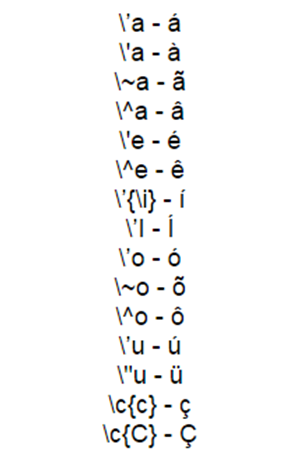
\includegraphics[scale=1.0]{USPSC-img/USPSC-AcentuacaoLaTeX.png} \\
	Fonte: \citeonline{comandos}
	\end{center}	
\end{figure}

\chapter{Símbolos úteis em \LaTeX}
\begin{figure}[H]
	\begin{center}
		\caption{\label{fig_anexoc}Símbolos úteis em \LaTeX}
		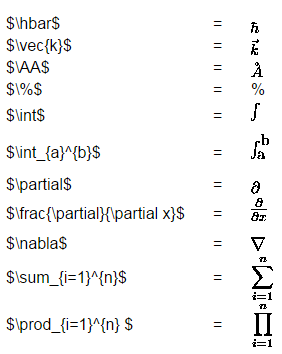
\includegraphics[scale=1.0]{USPSC-img/USPSC-SimbolosUteis.png} \\
		Fonte: \citeonline{comandos}
	\end{center}	
\end{figure}


\chapter{Letras gregas em \LaTeX}
\begin{figure}[H]
	\begin{center}
		\caption{\label{fig_anexod}Letras gregas em \LaTeX}
		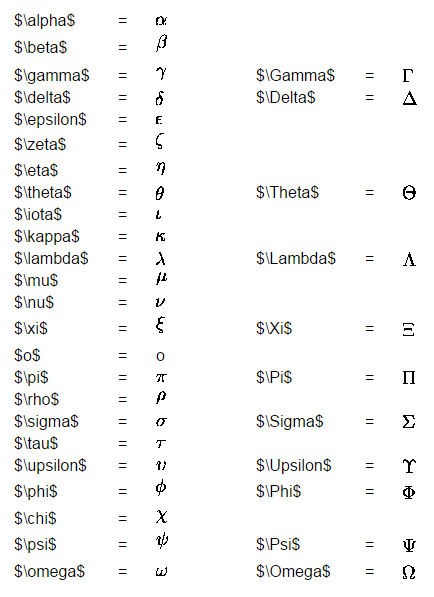
\includegraphics[scale=1.0]{USPSC-img/USPSC-LetrasGregas.png} \\
		Fonte: \citeonline{comandos}
	\end{center}	
\end{figure}

\end{anexosenv}


%---------------------------------------------------------------------
% INDICE REMISSIVO
%--------------------------------------------------------------------
%%% USPSC-IndicexRemissivosTutorial.tex
% ---
% Inicia os Índices Remissivos
% ---
%---------------------------------------------------------------------
% INDICE REMISSIVO
%--------------------------------------------------------------------
\phantompart
\printindex
%---------------------------------------------------------------------

\phantompart
\printindex
%---------------------------------------------------------------------


\end{document}
